\documentclass[final]{ukthesis}
%you must include these 2 packages.
\usepackage[pdfauthor={your name},
            pdftitle={The Title},
            pdfsubject={The Subject},
            pdfkeywords={Some Keywords},
            pdfproducer={Latex with hyperref},
            pdfcreator={latex->dvips->ps2pdf},
            pdfpagemode=UseOutlines,
            bookmarksopen=true,
            letterpaper,
            bookmarksnumbered=true]{hyperref}
\usepackage{memhfixc}

\DisemulatePackage{setspace}
\usepackage{setspace}

\let\footruleskip\undefined
\usepackage{fancyhdr}
\pagestyle{fancy}
\fancyhf{}
%\rhead{\leftmark}
\cfoot{\thepage}
%%%%%%%%%%%%%%%%%%%%%%%%%%%%%%%%%%%%%%%%%%%%%%%%

\let\proof\relax
\let\endproof\relax

\usepackage{amssymb,setspace}
\usepackage{xcolor}
\usepackage{url}
\usepackage{makeidx}
\usepackage{amsmath}
\usepackage{amsthm}
\usepackage{amsfonts}
\usepackage{caption}
\usepackage{subcaption}
\usepackage{multicol}
\usepackage{multirow}
\usepackage{graphicx}
\usepackage{float}
%\usepackage{subfig}
\usepackage{enumitem}

\usepackage{tikz}
\usepackage{verbatim}
\usetikzlibrary{shapes}
\usetikzlibrary{snakes}
\usetikzlibrary{arrows}
\usepackage{framed}
\usepackage{changepage}
\usepackage{tabularx}
\usepackage{listings}
\usepackage[algoruled,linesnumbered,lined,boxed]{algorithm2e}

\usepackage[normalem]{ulem}
\usetikzlibrary{arrows}

\tikzset{
	main node/.style={circle,draw,font=\small},
	rectangle/.style={font=\small},
	itria/.style={
  	draw,shape border uses incircle,
  	isosceles triangle,shape border rotate=90,yshift=-1.05cm
	},
	subtree/.style  = {isosceles triangle, draw=black, align=center, minimum height=0.4cm, 
		minimum width=0.8cm, shape border rotate=90, anchor=north}
}


\makeatletter

\newcommand{\ignore}[1]{}
\newcommand{\removelatexerror}{\let\@latex@error\@gobble}
\makeatother

\newcommand{\ifLparse}{\operatorname{:-}}
\newcommand\numberthis{\addtocounter{equation}{1}\tag{\theequation}}

\newcommand{\cA}{\mathcal{A}}
\newcommand{\cI}{\mathcal{I}}
\newcommand{\cD}{\mathcal{D}}
\newcommand{\CD}{\mathit{CD}}
\newcommand{\cX}{\mathcal{X}}
\newcommand{\cL}{\mathcal{L}}
\newcommand{\cV}{\mathcal{V}}
\newcommand{\cN}{\mathcal{N}}
\newcommand{\cC}{\mathcal{C}}
\newcommand{\cF}{\mathcal{F}}
\newcommand{\bbN}{\mathbb{N}}
\newcommand{\bbI}{\mathbb{I}}
\newcommand{\Iss}{\mathit{Iss}}
\newcommand{\ninst}{\mathit{NonInst}}
\newcommand{\Inst}{\mathit{Inst}}
\newcommand{\form}{\mathit{form}}
\newcommand{\anc}{\mathit{Anc}}
\newcommand{\WS}{\mathit{WS}}
\newcommand{\HB}{\mathit{HB}}
\newcommand{\bda}{\mathit{Borda}^{\mathit{ev}}_{\mathit{CI-UP}}}
\newcommand{\iss}{\mathit{Iss}}
\newcommand{\cP}{\mathcal{P}}
\newcommand{\iTran}{\textit{Transportation}}
\newcommand{\iDest}{\textit{Destination}}
\newcommand{\itiff}{\textit{iff}}
\newcommand{\IF}{\textit{if}}
\newcommand{\true}{\textit{true}}
\newcommand{\false}{\textit{false}}
\newcommand{\yes}{\textit{yes}}
\newcommand{\no}{\textit{no}}
\newcommand{\PS}{\mathit{PS}}
\newcommand{\At}{\mathit{At}}
\newcommand{\Comp}{\mathit{Comp}}
\newcommand{\Comps}{\mathit{Comps}}
\newcommand{\LCS}{\mathit{LCS}}
\newcommand{\GLP}{\textit{GLP}}
\newcommand{\PT}{\textit{PT}}
\newcommand{\vph}{\mathit{\varphi}}
\newcommand{\glp}{\textit{glp}}
\newcommand{\ASO}{\mathit{ASO}}
\newcommand{\LP}{\mathit{LP}}
\newcommand{\TP}{\mathit{TP}}
\newcommand{\TD}{\mathit{TD}}
\newcommand{\IO}{\mathit{IO}}
\newcommand{\SD}{\mathit{SD}}
\newcommand{\PATH}{\mathit{PATH}}
\newcommand{\NP}{\mathit{NP}}
\newcommand{\coNP}{\mathit{coNP}}
\newcommand{\AI}{\mathit{AI}}
\newcommand{\Domin}{\mathit{Domin}}
\newcommand{\Pa}{\mathit{Pa}}
\newcommand{\gen}{\mathit{gen}}
\newcommand{\PREF}{\mathit{pref}}
\newcommand{\Asst}{\mathit{Asst}}
\newcommand{\clingo}{\textit{clingo}}
\newcommand{\clingcon}{\textit{clingcon}}
\newcommand{\toulbar}{\textit{toulbar}}
\newcommand{\clasp}{\textit{clasp}}
\newcommand{\Eval}{\mathit{Eval}}
\newcommand{\incon}{\mathit{incon}}
\newcommand{\veps}{\mathit{\varepsilon}}
\newcommand{\cE}{\mathcal{E}}
\newcommand{\PL}{\mathit{PL}}
\newcommand{\NEQ}{\mathit{NEQ}}
\newcommand{\EQ}{\mathit{EQ}}
\newcommand{\RC}{\mathit{RC}}
\newcommand{\MH}{\mathit{MH}}
\newcommand{\poly}{\mathit{poly}}
\newcommand{\DTIME}{\mathit{DTIME}}
\newcommand{\UI}{\textit{UI}}
\newcommand{\CI}{\textit{CI}}
\newcommand{\FP}{\textit{FP}}
\newcommand{\UP}{\textit{UP}}
\newcommand{\CP}{\textit{CP}}
\newcommand{\PCPT}{\textit{PCPT}}
\newcommand{\CPT}{\textit{CPT}}
\newcommand{\BL}{\mathit{BL}}
\newcommand{\BR}{\mathit{BR}}
\newcommand{\cond}{\mathit{cond}}
\newcommand{\pc}[1]{{\color{blue}{#1}}}
\newcommand{\tsc}[1]{\textsc{#1}}
\newcommand{\tit}[1]{\textit{#1}}
\newcommand{\tbf}[1]{\textbf{#1}}
\newcommand{\secref}[1]{Section~\ref{sec:#1}}
\newcommand{\chref}[1]{Chapter~\ref{ch:#1}}
\newcommand{\figref}[1]{Figure~\ref{fig:#1}}
\newcommand{\tblref}[1]{Table~\ref{tbl:#1}}
\newcommand{\defref}[1]{Definition~\ref{def:#1}}
\newcommand{\thmref}[1]{Theorem~\ref{thm:#1}}
\newcommand{\lemref}[1]{Lemma~\ref{lem:#1}}
\newcommand{\propref}[1]{Proposition~\ref{prop:#1}}
\newcommand{\algref}[1]{Algorithm~\ref{alg:#1}}
\newcommand{\eqtref}[1]{Equation~\ref{eq:#1}}
\newcommand{\corref}[1]{Corollary~\ref{cor:#1}}
\newcommand{\sigmap}[1]{\mathit{\Sigma^P_{#1}}}
\newcommand{\piptwo}{\mathit{\Pi^P_2}}
\newcommand{\deltap}[1]{\mathit{\Delta^P_{#1}}}
\newcommand{\pip}[1]{\Pi^P_{#1}}
\newcommand{\SWF}{\it{SWF}}
\newcommand{\SCF}{\it{SCF}}
\newcommand{\topFunc}{\it{top}}
\newcommand{\tc}[1]{\textcolor{blue}{#1}}
\newcommand{\redtext}[1]{{\color{red}{#1}}}
\newcommand{\bluetext}[1]{{\color{blue}{#1}}}
\newcommand{\tr}{\mathit{\triangleright}}
\newcommand{\trir}{\mathit{\triangleright}}
\newcommand{\la}{\mathit{\langle}}
\newcommand{\ra}{\mathit{\rangle}}
\newcommand{\bV}{\textbf{V}}
\newcommand{\bD}{\textbf{D}}
\newcommand{\bT}{\textbf{T}}
\newcommand{\bS}{\textbf{S}}
\newcommand{\bU}{\textbf{U}}
\newcommand{\bu}{\textbf{u}}
\newcommand{\bY}{\textbf{Y}}
\newcommand{\by}{\textbf{y}}
\newcommand{\bZ}{\textbf{Z}}
\newcommand{\bz}{\textbf{z}}
\newcommand{\bX}{\textbf{X}}
\newcommand{\bx}{\textbf{x}}
\newcommand{\Dom}{\it{Dom}}
\newcommand{\bP}{\textbf{P}}
\newcommand{\bNP}{\textbf{NP}}
\newcommand{\bPH}{\textbf{PH}}
\newcommand{\bSharpP}{\textbf{\#P}}
\newcommand{\bCoNP}{\textbf{coNP}}
\newcommand{\bPSPACE}{\textbf{PSPACE}}
\newcommand{\bDTIME}{\textbf{DTIME}}
\newcommand{\bNTIME}{\textbf{NTIME}}
\newcommand{\cPP}{\mathcal{PP}}
\newcommand{\PCF}{\mathit{PCF}}
\newcommand{\walk}{\mathit{walk}}
\newcommand{\bike}{\mathit{bike}}
\newcommand{\car}{\mathit{car}}
\newcommand{\public}{\mathit{public}}
\newcommand{\taxi}{\mathit{taxi}}
\newcommand{\gas}{\mathit{gas}}
\newcommand{\wait}{\mathit{wait}}
\newcommand{\SUM}{\mathit{sum}}
\newcommand{\MAX}{\mathit{max}}
\newcommand{\MIN}{\mathit{min}}
\newcommand{\AVG}{\mathit{avg}}
\newcommand\nop[1]{}
\makeatletter
\newcommand*{\rom}[1]{\expandafter\@slowromancap\romannumeral #1@}
\makeatother

%\urldef{\mails}\path|liu@cs.uky.edu, mirek@cs.engr.uky.edu|
\urldef{\mails}\path|liu@cs.uky.edu|

\newtheorem{thm}{Theorem}
\newtheorem{prop}{Proposition}
\newtheorem{cor}[thm]{Corollary}
\newtheorem{lem}{Lemma}
\theoremstyle{definition}
%\newtheorem{definition}[thm]{Definition} % definition numbers are dependent on theorem numbers
\newtheorem{definition}{Definition} % definition numbers are independent on theorem numbers
\newtheorem{ex}{Example}
\newtheorem{observation}{Observation}

\newenvironment{remark}[1][Remark]{\begin{trivlist}
\item[\hskip \labelsep {\bfseries #1}]}{\end{trivlist}}

\usepackage[normalem]{ulem}
\usetikzlibrary{arrows}

\newenvironment{subcase}{\begin{adjustwidth}{0.5cm}{}}{\end{adjustwidth}}
\providecommand{\shortcite}[1]{\cite{#1}}


\doublespacing

\begin{document}
%author data
\author{Xudong Liu}
\title{MODELING, LEARNING AND REASONING ABOUT PREFERENCE TREES OVER COMBINATORIAL DOMAINS}
\abstract{In my Ph.D. dissertation, I have studied problems arising in various aspects of preferences:
preference modeling, preference learning, and preference reasoning, 
when preferences concern outcomes ranging over combinatorial domains.
Preferences is a major research component
in artificial intelligence (AI) and decision theory, and is closely related to the 
social choice theory considered by economists and political scientists. 
In my dissertation, I have exploited emerging connections between 
preferences in AI and social choice theory. 
Most of my research is on qualitative preference representations that extend and combine
existing formalisms such as conditional preference nets, 
lexicographic preference trees, answer-set optimization programs,
possibilistic logic, and conditional preference networks; on 
learning problems that aim at discovering qualitative preference models and 
predictive preference information from practical data; and on
preference reasoning problems centered around qualitative preference optimization 
and aggregation methods.
Applications of my
research include recommender systems, decision support tools, multi-agent systems,
and Internet trading and marketing platforms.
}
\advisor{Miroslaw Truszczynski}
\keywords{preferences, decision theory, social choice theory,
					knowledge representation and reasoning,
					computational complexity,
					artificial intelligence}
\dgs{Miroslaw Truszczynski}
%the title pages
\frontmatter
\maketitle

\begin{dedication}
	To my family, especially to my son Adam (Shude) Liu.

\end{dedication}
\begin{acknowledgments}
	I want to thank Dr. Truszczynski, other professors on my committee board, my colleagues,
my parents, my wife and son, and my friends.

\end{acknowledgments}
\rhead{}
\tableofcontents\clearpage
\rhead{\leftmark}
\listoffigures\clearpage
\listoftables\clearpage
%----------------------------------------------
\mainmatter

\chapter{Introduction\label{ch:intro}}
%%%% INTRO FUN! %%%%%%
%% start of comments
%\tc{
%	Here I will talk about the field I am working in, namely, 
%	preferences in Artificial Intelligence and 
%	Social Choice.
%	I will discribe the problems I am interested in in the field and explain
%	why these problems are interesting, important and
%	challenging for researchers to study. I will briefly mention other
%	people's work.
%	I will outline this document at the end of this section.
%}
%% end of comments
Preferences are ubiquitous.
They arise when we select ice-cream flavors, vote for candidates for an office,
and buy cars.
Preferences have spurred research in areas such as 
artificial intelligence, psychology, economics, and operations research.
Specifically, there has been growing interest in research problems on
preferences in contexts such as knowledge representation and reasoning, constraint 
satisfaction, decision making, and social choice theory. 
My research focuses on problems in preference modeling, 
reasoning and learning.

Preferences can be represented in a \tit{quantitative} and \tit{qualitative} manner.
For the former, agents express preferences in a numerical form of
a value function that precisely assesses the degree of satisfaction
of objects
(often called \textit{outcomes} or \textit{alternatives}).
Specifying preferences as value functions on alternatives
is feasible for humans in some situations, e.g., 
when the number of alternatives is limited.
In other circumstances, particularly when the number of alternatives is large,
people often cannot express their 
preferences directly and accurately as value 
functions \cite{Domshlak20111037}.
%due to the burden of deciding the value function for
%a large number of alternatives \cite{Domshlak20111037}.

Assume an agent is given three flavors of ice-cream:
$strawberry$, $chocolate$ and $vanilla$, and is asked to describe 
her preference among them.
The agent could think of a value function that
assigns quantities (\textit{utilities}) to each outcome
based on a scale from 1 to 10, with 10 representing the most satisfaction.
For instance, the agent could give the following value function:
\begin{center}
	$strawberry \mapsto 6$, $chocolate \mapsto 9$ and $vanilla \mapsto 3$.
\end{center}
This function shows that the favorite alternative to the agent is
$chocolate$ (it has the highest utility), and
$strawberry$ is preferred over $vanilla$.

Instead of rating alternatives quantitatively, it is
often easier and more intuitive to give preferential information
in a qualitative way,
so that to specify a binary preference relation.
Thus, the same agent could rank the flavors as the following
preference order:
\begin{center}
	$chocolate \succ strawberry \succ vanilla$.
\end{center}
Note that one can obtain the qualitative preferences from
the value function, but not vice versa.
My research deals with qualitative preference relations.

%Provided with preferences learned and presented in a formalism,
%what can we say about the agent's preferences over outcomes?
Preferences play an essential role in areas that involve making
decision, such as decision theory and social choice theory.
Once we have preferences of a user or users, we can reason about
the preferences to support decision making.
In general, preference reasoning problems can be classified
based on the number $n$ of agents from which the preferences are gathered:
\begin{enumerate} \itemsep -4pt
	\item $n=1$: individual decision making,
	\item $n>1$: collaborative decision making.
\end{enumerate}
In case $n=1$, we focus on optimization of the agent's preferences and
help her make a better decision by, for example, computing an optimal
alternative or comparing two given alternatives.  For the case
where $n>1$, it is important to calculate
a consensus (e.g., a winning outcome or ranking)
of the group of agents.

One of the problems in preference reasoning is to
aggregate preferences of a group of
agents. The problem is central to collective decision making and has been studied
extensively in social choice theory. 
Let us consider a scenario, where we are
given a set of alternatives $X = \{ a,b,c,d,e \}$ and a set $P_X$ of 10 
preferences (called \tit{votes}) as follows.
	\begin{center}
		5 : $a > c > b > e > d$,\\
		3 : $b > a > e > c > d$,\\
		2 : $c > d > b > a > e$.
	\end{center}
	
Note that the integer associated with every preference order
is the number of agents sharing that same preference.
We are asked to compute the winning alternative according to some aggregation rule. 
Plurality, veto and Borda are examples of commonly used voting rules.
For instance, Borda rule assigns score $m-i$ to the $i$th ranked 
alternative, where $m$ is the number of alternatives.
Thus, the winner is the alternative with the highest score.
We compute that the Borda winner for $P_X$ is $a$, since its 
score $31$ is the highest, followed by candidates $b$ and $c$
with the second highest score $26$.

While in the cases when the
number of alternatives is small the preference-aggregating 
problems (dominance testing, winner determination,
etc) have received wide attention in the literature,
the problems concerning preferences over \tit{combinatorial
domains}, which typically contain large numbers of outcomes, 
have not been investigated as much.

For example, a taxi company plans to purchase a fleet of cars.
The features (or, as we will say, attributes) that will be
taken into account are \tit{BodyType}, \tit{Capacity},
\tit{Make}, \tit{Price}, and \tit{Safety}.  
Each attribute has a domain of values that it can take, e.g.,
\tit{BodyType} may have four values \tit{minivan}, \tit{sedan}, \tit{sport}, and \tit{suv}.
There could be hundreds or thousands of cars,
described by different combinations of values on these five attributes, 
even for a relatively small number of attributes, and
the agents will soon find it impossible to enumerate all of
them from the most preferred to the least.

Consequently, an expressive yet concise representation is needed to specify
preferences over combinatorial alternatives.
Such preference formalisms are often categorized into \tit{logical models} and
\tit{graphical models}.
Logical models include penalty logic (\tit{Pen-logic}) \cite{haddawy1992representations}, 
possibilistic logic (\tit{Poss-logic}) \cite{DuboisLP91},
qualitative choice logic (\tit{Qual-logic}) \cite{brewka2004qualitative},
conditional preference theories (\tit{CP-theories}) \cite{Wilson04extendingcp-nets},
and answer set optimization (\tit{ASO}) \cite{Brewka:ASO},
whereas graphical models found in the literature include
generalized additive independence networks (GAI-nets) \cite{BacchusG95,LIP61766},
lexicographic preference trees (\tit{LP-trees}) \cite{booth:learningLP,conf/adt13/LiuT},
conditional preference networks (\tit{CP-nets}) \cite{Kaci:Pref},
conditional preference networks with tradeoffs (\tit{TCP-nets}) \cite{BrafmanD02:TCP},
and conditional importance networks (\tit{CI-nets}) \cite{Kaci:Pref}.

Once we fix a preference formalism, say $\cF$, in which preferences of agents
are specified, eliciting and learning preference expressions in $\cF$ from agents
becomes a fundamental problem.
Different techniques have been proposed to preference learning
in $\cF$
such as \tit{active learning} (or \tit{preference elicitation}) and 
\tit{passive learning} \cite{Furnkranz:pref_learning}.
In the process of
active learning, the algorithm iteratively asks the user for a pairwise 
preference between two given outcomes and constructs
an instance of $\cF$ as more preferences are elicited.
For passive learning, the learning algorithm assumes that a set of
pairwise preferences are obtained over a period of time and builds an instance
of $\cF$ with no more information from the user.

My research has centered around the language of LP-trees.
Extending LP-trees, I have proposed two new tree-like preference formalisms:
partial lexicographic preference trees (\tit{PLP-trees}) \cite{conf/aaai15/LiuT}
and preference trees (\tit{P-trees}) \cite{fraser1994,liu2014preference,conf/adt15/liuT}.
For example, the language of P-trees exploits a natural way humans apply to
express preference information in the setting of combinatorial domains.
Often a human agent would first consider the most desired \tit{criterion},
possibly represented by a propositional formula $\varphi$.
Outcomes that agree with it are preferred to those that do not.  
Then, the same mechanism is applied recursively to further discriminate the 
outcomes that satisfy $\varphi$ and those that falsify $\varphi$.
This process ends up with a structured preference system that always
induces a total preorder.

My research on tree-like preference formalisms can be categorized into
three main directions -- preference modeling, learning and reasoning.

\smallskip \noindent \textbf{Preference Modeling \ }
\noindent My research formally proposed 
PLP-trees \cite{conf/aaai15/LiuT} and P-trees \cite{liu2014preference,conf/adt15/liuT}.
In particular, I studied
the relationship between P-trees and other existing preference languages, and
showed that P-trees extend
LP-trees, possibilistic logic, and ASO rules.
Moreover, my work established computational complexity results of commonly considered decision
problems in the setting of P-trees, such as \textit{dominance testing} 
\textit{optimality testing}, and
\textit{optimality testing w.r.t a property}.

\smallskip \noindent \textbf{Preference Learning \ }
Given a set of pairwise preferences between alternatives, 
called \textit{examples}, acquired from the user,
it is important to learn (i) a PLP-tree, 
preferably of a small size, 
consistent with a dataset of examples, and (ii) a PLP-tree correctly
ordering as many of the examples as possible in case
of inconsistency. In my work, I stuied both these problems \cite{conf/aaai15/LiuT}. 
I established complexity results
for them and, in each case where the problem
is in the class P, proposed a polynomial time algorithm.
On the experimentation side,
I have designed and implemented algorithms, using both
Answer-Set Programming (ASP) and approximation methods, to learn PLP-trees 
and forests of these trees in the passive learning setting.
To facilitate experimentation, I developed several datasets
based on classification datasets such as \tit{Library for Preferences},
\tit{Preference Learning Site}, and \tit{UCI Machine Learning Repository}.
To evaluate the effectiveness and feasibility of our own models, I 
compared them with machine learning models, such as 
decision trees and random forests.

\smallskip \noindent \textbf{Preference Aggregation  \ }
In this area, I investigated two preference-aggregation 
problems, the \emph{winner} problem and the \emph{evaluation} problem,
based on \textit{positional scoring rules} (such as $k$-approval and Borda) 
when votes in elections are given as LP-trees \cite{abs/ijcai13dc/Liu,conf/adt13/LiuT}. 
My work brought new computational complexity results of these problems, and
provided computational methods to model and solve the problems using
\tit{answer set programming} (ASP) and \tit{weighted partial maximum satisfiability} (WPM).
%%%%%%%% FUTURE WORK
%I am also studying problems related to vulnerability of collective decisions under 
%misrepresentation of preferences specified over combinatorial domains.
%For instance, the \textit{coalitional manipulation problem}
%asks to decide if a small coalition set of manipulative
%agents can make some candidate a winner.
%I am examining positional scoring rules,
%comparison-based rules (e.g., the Copeland, Simpson and Maximin rules), and 
%distance-based rules (e.g., the Kemeny and Dodgson rules), for LP-trees,
%and will extend these results to elections over complicated domains to more general cases.
%%%%%%%% FUTURE WORK

%\smallskip \noindent \textbf{Application of Preferences  \ }
%Besides addressing computational problems on preferences,
%I have applied the theory into practical problem solving.
%One collaboration with research peers resulted in a refereed publication \cite{conf/adt13/Spradling},
%where we introduced a new variant of hedonic coalition formation games in which agents 
%have preferences on their own coalitions.
%In another collaborative effort with researchers in the Palo Alto Research Center,
%we designed and developed software modules for representing and reasoning about user 
%constraints and preferences in a trip planning setting, which is prepared
%for publication.

%%%%%%%% FUTURE WORK
%My long-term research goal is to study computational problems related to preferences, and 
%develop applications that help people or software agents make better decisions.
%Particularly, I intend to embed theories and practices on preferences into areas including
%data science, automated planning and scheduling, and database systems.
%%%%%%%% FUTURE WORK

The outline of the remainder of this thesis is the following. 
In \chref{preliminary}, I present necessary technical preliminaries
including binary relations, order theory, and computational complexity theory.
In \chref{relwork}, I go through related work that proposed
approaches to preference modeling and reasoning
in artificial intelligence and social choice theory.
In Chapters 4 to 7, I discuss results of my work on
modeling, learning and reasoning about preferences over combinatorial domains.
I conclude with a brief note in \chref{summary} on my ongoing research,
as well as on possible directions of future work.

%Note the copyright notice at the end of each chapter.
\copyrightnotice

\chapter{Technical Preliminaries\label{ch:preliminary}}
%%%%% Techinical Preliminaries %%%%%

In this section I will give an overview of
mathematical and computational concepts
that I will use throughout the rest of this document. 
First, since I consider preference relations that are modeled
as binary relations,
I recall the definitions of binary relations and their key
properties.
I then define several types of preference relations in terms of
these properties.
Second, I review combinatorial domains as I am interested in
preferences over combinatorial domains.
Third, I introduce propositional logic to show how propositional
formulas are used to compactly represent outcomes.
Finally, I review concepts in computational complexity theory,
as they are useful in describing the hardness of problems
involving reasoning about preferences.

\section{Relations and Orders \label{sec:relations}}


\begin{definition}
	Let $A$ and $B$ be two sets of elements.  A \textit{binary relation} $R$ between $A$ and $B$
	is a subset of the Cartesian product of $A$ and $B$, that is,
	\begin{center}
		$R \subseteq A \times B$.
	\end{center}
\end{definition}


The following properties of binary relations are particularly relevant for modeling preferences.
\begin{definition}
	Let $R$ be a binary relation over a set $O$ of objects ($R \subseteq O \times O$).
	I say that $R$ is
	\begin{enumerate} \itemsep -4pt
		\item reflexive if for every $o \in O$, $(o,o) \in R$.
		\item irreflexive if for every $o \in O$, $(o,o) \not \in R$.
		\item total if for every $o_1,o_2 \in O$, $(o_1,o_2) \in R$ or $(o_2,o_1) \in R$.
		\item transitive if for every $o_1,o_2,o_3 \in O$, if $(o_1,o_2) \in R$ and $(o_2,o_3) \in R$, 
					then $(o_1,o_3) \in R$.
		\item symmetric if for every $o_1,o_2 \in O$, if $(o_1,o_2) \in R$, then $(o_2,o_1) \in R$.
		\item antisymmetric if for every $o_1,o_2 \in O$, if $(o_1,o_2) \in R$ and $(o_2,o_1) \in R$, then $o_1=o_2$.
%		\item asymmetric: $\forall o,o' \in O$, if $oRo'$, $\neg o'Ro$.
	\end{enumerate}
\end{definition}

For instance, assuming that $\bbN=\{1,2,\ldots\}$ is the set of positive integers,
the \tit{less-than-or-equal-to} relation $\leq$ over $\bbN$ is reflexive,
total, transitive and antisymmetric, while the \tit{less-than} relation
$<$ over $\bbN$ is irreflexive, transitive and antisymmetric.


\begin{definition}
\label{def:orders}
	A binary relation over $O$ is a \textit{partial preorder} if it is reflexive and transitive,
	a \textit{total preorder} if it is a partial preorder that is total,
	a \textit{partial order} if it is a partial preorder that is antisymmetric,
	and a \textit{total order} if it is a partial order that is total.
\end{definition}

I use preorders to model preference relations.
Thus, when I describe a preference order, I have in mind a relation
that is a partial preorder.
Given two objects $o$ and $o'$,
I sometimes need to say that $o'$ is at least as good as $o$ or,
that $o'$ is strictly preferred over $o$.
In some situations, due to 
lack of information about the two objects at hand, we
cannot determine which object is preferred over the other, and
speak about the objects being incomparable.
Formally, I have the following definitions.
\begin{definition}
	Let $O$ be a set of objects, and $o$ and $o'$ two objects in $O$.
	Let $\succeq$ be a preference relation that is a partial preorder	over $O$.
	I say that $o'$ is weakly preferred to $o$ if $o' \succeq o$.
	Object $o'$ is strictly preferred to $o$, $o' \succ o$, if $o' \succeq o$ and $o \not \succeq o'$.
	Object $o'$ is equivalent with $o$, $o' \approx o$, if $o' \succeq o$ and $o \succeq o'$.
	Object $o'$ is incomparable with $o$, $o' \bowtie o$, if $o' \not \succeq o$ and $o \not \succeq o'$.
\end{definition}

\nop{\tc{Examples of these orders.}}
I illustrate these notions with several examples of preorders (preference orders)
in \figref{relations}.
I assume that a directed edge is from a less preferred object to
a more preferred one.
It is clear that the relation in \figref{partpre} is a partial 
preorder, \figref{totalpre} a total preorder, \figref{partord} a partial
order, and \figref{totalord} a total order.


\begin{figure}[ht]
   \small
  \centering
		\begin{subfigure}[b]{0.45\textwidth}
	  	\centering
		  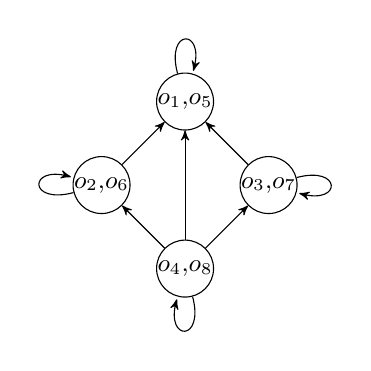
\begin{tikzpicture}[->,>=stealth',node distance=1.5cm,main node/.style={circle,draw,font=\small}]
		    \node[main node,inner sep=0pt] (1)                    {$o_1,\!o_5$};
				\node[main node,inner sep=0pt] (2) [below left of=1]  {$o_2,\!o_6$};
		  	\node[main node,inner sep=0pt] (3) [below right of=1] {$o_3,\!o_7$};
		  	\node[main node,inner sep=0pt] (4) [below right of=2] {$o_4,\!o_8$};
		
		    \path[every node/.style={font=\sffamily\small}]
		      (4) edge (2)
		      (4) edge (3)
		      (2) edge (1)
		      (3) edge (1)
		      (4) edge (1)
					(1) edge [loop above] (1)
					(2) edge [loop left] (2)
					(3) edge [loop right] (3)
					(4) edge [loop below] (4);
		  \end{tikzpicture}
      \caption{partial preorder\label{fig:partpre}}
    \end{subfigure}
    \begin{subfigure}[b]{0.45\textwidth}
	  	\centering
		  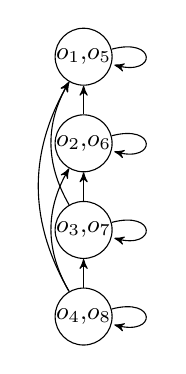
\begin{tikzpicture}[->,>=stealth',node distance=1.1cm,main node/.style={circle,draw,font=\small}]
		    \node[main node,inner sep=0pt] (1)              {$o_1,\!o_5$};
				\node[main node,inner sep=0pt] (2) [below of=1] {$o_2,\!o_6$};
		  	\node[main node,inner sep=0pt] (3) [below of=2] {$o_3,\!o_7$};
		  	\node[main node,inner sep=0pt] (4) [below of=3] {$o_4,\!o_8$};
		
		    \path[every node/.style={font=\sffamily\small}]
		      (4) edge (3)
		      (4) edge [bend left] (2)
		      (4) edge [bend left] (1)
		      (3) edge (2)
		      (3) edge [bend left] (1)
		      (2) edge (1)
					(1) edge [loop right] (1)
					(2) edge [loop right] (2)
					(3) edge [loop right] (3)
					(4) edge [loop right] (4);
		  \end{tikzpicture}
      \caption{total preorder\label{fig:totalpre}}
    \end{subfigure} \\
    \begin{subfigure}[b]{0.45\textwidth}
	  	\centering
		  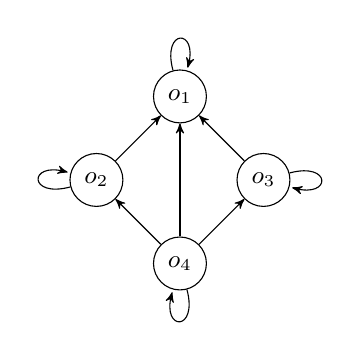
\begin{tikzpicture}[->,>=stealth',node distance=1.5cm,main node/.style={circle,draw,font=\small}]
		    \node[main node] (1) {$o_1$};
				\node[main node] (2) [below left of=1] {$o_2$};
		  	\node[main node] (3) [below right of=1] {$o_3$};
		  	\node[main node] (4) [below right of=2] {$o_4$};
		
		    \path[every node/.style={font=\sffamily\small}]
		      (4) edge (2)
		      (4) edge (3)
		      (2) edge (1)
		      (3) edge (1)
		      (4) edge (1)
					(1) edge [loop above] (1)
					(2) edge [loop left] (2)
					(3) edge [loop right] (3)
					(4) edge [loop below] (4);
		  \end{tikzpicture}
      \caption{partial order\label{fig:partord}}
    \end{subfigure}
    \begin{subfigure}[b]{0.45\textwidth}
	  	\centering
		  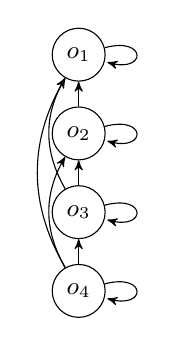
\begin{tikzpicture}[->,>=stealth',node distance=1cm,main node/.style={circle,draw,font=\small}]
		    \node[main node] (1) {$o_1$};
				\node[main node] (2) [below of=1] {$o_2$};
		  	\node[main node] (3) [below of=2] {$o_3$};
		  	\node[main node] (4) [below of=3] {$o_4$};
		
		    \path[every node/.style={font=\sffamily\small}]
		      (4) edge (3)
		      (4) edge [bend left] (2)
		      (4) edge [bend left] (1)
		      (3) edge (2)
		      (3) edge [bend left] (1)
		      (2) edge (1)
					(1) edge [loop right] (1)
					(2) edge [loop right] (2)
					(3) edge [loop right] (3)
					(4) edge [loop right] (4);
		  \end{tikzpicture}
      \caption{total order\label{fig:totalord}}
    \end{subfigure}
  \caption{Binary relations}
  \label{fig:relations}
\end{figure}


\begin{definition}
	Let $R$ and $R'$ be two binary relations,
	$R'$ \textit{extends} $R$ if $R \subseteq R'$.
\end{definition}

As an example of relation extensions, I consider the partial order $\succeq$ 
in \figref{partord}.
Since $o_2 \bowtie o_3$, I have in total two extensions:
\begin{center}
	$o_1 \succeq o_2 \succeq o_3 \succeq o_4$,\\
	$o_1 \succeq o_3 \succeq o_2 \succeq o_4$.
\end{center}

\begin{definition}
	Let $\succeq$ be a preference relation over $O$,
	$o \in O$ is \textit{optimal} if there does not exist $o' \in O$
	such that $o' \succ o$.
\end{definition}
For instance, object $o_1$ is optimal in the partial preorder
shown in \figref{partpre}.



\section{Combinatorial Domains \label{sec:comb_domains}}
One scenario when decision problems involving preferences are difficult is when outcomes
are described as combinations of attribute values from finite domains.
Take the domain of cars as an example, where the attributes I care about are
\tit{Price}, \tit{Safety}, and \tit{Capacity}.
Every attribute has a finite domain of values:
\tit{Price} with domain $\{$\tit{low,med,high,vhigh}$\}$,
\tit{Safety} with domain $\{$\tit{low,med,high}$\}$, and
\tit{Capacity} with domain $\{$\tit{2,5,7m}$\}$.
Since these are the only aspects of a car we care about, cars can be
described as vectors of values from these domains.
For instance, vector $\la$\tit{med,high,7m}$\ra$ represents
a car that is medium priced, medium level of safety, and can carry seven
or more people.
Even in this simple example, there are already 36 configurations describing
different types of cars.

\begin{definition}
	Let $\cI$ be a set of attributes $\{X_1,\ldots,X_p\}$, each attribute $X_i$
	associated with a finite domain $\Dom(X_i)$.
	A \textit{combinatorial domain} $\CD(\cI)$ is a set of 
	combinations of values from $\Dom(X_i)$:
	\begin{center}
		$\CD(\cI) = \prod_{X_i \in \bV} \Dom(X_i)$.
	\end{center}
\end{definition}

%An example of combinatorial domain is the space of \textit{subsets} of $\bV$.
%In this case, $\bD$ is a set of binary domains, and a tuple
%$t \in \bT$ is a combination of 0's and 1's.
%Note that $0_i \in t$ means that $X_i$ is not in the corresponding subset,
%and that $1_i \in t$ means that $X_i$ is.
%It is not hard to see that
%the set $\bT$ of tuples is exactly the space $\bS$ of subsets of $\bV$.

We call the elements of $\CD(\cI)$ outcomes.
Clearly, the size of $\CD(\cI)$ is exponential in $p$, the number of attributes.
The exponential growth of $|\CD(\cI)|$ makes it hard, if not impossible, for agents
to directly assess their preferences, even when each domain is binary and
there are as few as 6-7 attributes.
In many practical cases, hard constraints that can be modeled, for instance, 
by propositional formulas, are identified and imposed 
to eliminate the infeasible outcomes.



\section{Propositional Logic}
In this work, \tit{propositional logic} plays an important role in compactly representing
preferences over combinatorial domains.
Propositional logic \cite{heindiscrete}, or propositional calculus, is a logic language concerning
propositions (e.g., statements that are true or false) that are built upon atomic propositions
by means of logical connectives.
I first define the syntax of the language, that is, how formulas are constructed.
Then, I show its semantics, i.e., what it means for a formula to be true or false.

Propositions are represented as \tit{well-formed formulas}, or simply \tit{formulas} when no ambiguity.
Formulas are built from an alphabet of truth symbols ($\top$ and $\bot$),
variables (uppercase letters), connectives ($\neg$, $\land$, $\lor$, and $\rar$), and parantheses.
A \tit{formula} is either a truth symbol, a variable, or, if $\varphi$ and $\psi$ are formulas,
$(\neg \varphi)$, $(\varphi \lor \psi)$, $(\varphi \land \psi)$, and
$(\varphi \rar \psi)$. (Outside pair of parentheses are often left out.)
For example, if $X$ and $Y$ are formulas, I have that $X \land (X \rar \neg Y)$ is a formula.

%The meaning of any formula is its \tit{truth table}.
%The truth table enumerates \tit{truth assignments} to variables appearing in a formula to determine
%whether the formula is true or not.
%I have that the meaning of $T$ is true, and that of $F$ is false.
%For instance, the semantics of several formulas is given as a true table in \tblref{truth}.
%
%\begin{table}[ht]
%\centering
%	\begin{tabular}{ |c c|c c c c| }
%	  \hline
%	  $X$ & $Y$ & $\neg X$ & $X \land Y$ & $X \lor Y$ & $X \rar Y$ \\
%	  \hline
%		$T$ & $T$ & $F$ & $T$ & $T$ & $T$ \\
%	  \hline                            
%		$T$ & $F$ & $F$ & $F$ & $T$ & $F$ \\
%	  \hline                            
%		$F$ & $T$ & $T$ & $F$ & $T$ & $T$ \\
%	  \hline                            
%		$F$ & $F$ & $T$ & $F$ & $F$ & $T$ \\
%	  \hline
%	\end{tabular}
%	\caption{Truth table\label{tbl:truth}}
%\end{table}

A \tit{truth assignments} is a mapping $v$ from variables to \tit{T}
and \tit{F} values.
I now defines what it means for a truth assignment to \tit{satisfy} 
and \tit{falsify} a formula.
Let $v$ be a truth assignment, $X$ a variable, and $\varphi$ and $\psi$
propositional formulas.
First, I define that $v$ satisfies $X$, denoted by $v \models X$,
if $v$ has value \tit{T} on $X$; and that $v$ falsifies $X$, denoted 
by $v \not\models X$, if $v$ has value \tit{F} on $X$.
Then, I have $v \models \neg \varphi$
if  $v \not\models \varphi$ holds, $v \models \varphi \land \psi$
if $v \models \varphi$ and $v \models \psi$ hold, $v \models \varphi \lor \psi$
if $v \models \varphi$ or $v \models \psi$ holds, $v \models \varphi \rar \psi$
if $v \not\models \varphi$ holds or $v \models \psi$ holds.
I always have $v \models \top$ and $v \not\models \bot$.

A truth assignment can then be viewed an outcome in a combinatorial domain.
I view the values in the attribute domains as variables in propositional logic.
Any truth assignment $M$ over these variables represents an outcome $o$
in the following way.
A variable assigned \tit{True} (\tit{False}) in $M$ means corresponding 
attribute value is in $o$ (is not in $o$, respectively).
As a result, a formula provides a compact way of representing a set of, 
possibly exponentially many, outcomes.
Formula $\varphi$ represents the set of outcomes whose counterpart
truth assignments satisfy $\varphi$.
I consider the domain of cars as discussed in \secref{comb_domains}.
The car $\la$\tit{med,high,7m}$\ra$ in the combinatorial domain
is represented as a truth assignment over $10$ variables, because
there are $10$ attribute values.
I denote these variables by $L_P$, $M_P$, $H_P$, $V_P$,
$L_S$, $M_S$, $H_S$, $T_C$, $F_C$, and $S_C$, in order of the
values in attributes \tit{Capacity}, \tit{Price}, and \tit{Safety}.
This truth assignment sets \tit{True} on variables $M_P$,
$H_S$ and $S_C$, and \tit{False} on the others.
I see that not all truth assignments are legal.
Thus, I need a constraint that, for every attribute domain,
exactly one variable is true.  Such a constraint can be
expressed as a propositional formula $\Phi$.
Now it is clear that formula $\Phi \land ((H_P \land S_C) \lor (M_P \land M_S))$ precisely
and concisely represents the set of cars that have high price and
capacity of 7 or more, and cars that have medium price and medium
security.


\section{Computational Complexity Theory \label{sec:comp_theory}}
\nop{\tc{
Here I talk about complexity classes of interest, including
the classes P, NP, coNP, NP-complete, coNP-complete, NP-Hard, \#P, polynomial
hierarchy.
}}

Computer scientists looking for algorithms to solve computational problems
seek ways to classify problems according to their computational hardness
in terms of time (the number of instructions needed to solve the problem) 
or space (the size of memory needed to solve the problem).
In this section, I define classes of computational
complexity used for such classification.
I assume familiarity with the concept of the \textit{Turing machine} (TM).
The definition of this notion and other definitions discussed 
below can be found in complexity
books by Garey and Johnson \cite{gar-joh:b:int}; Lewis and Papadimitriou
\cite{Lewis:Comput}; and Arora and Barak \cite{Arora:Comput}.



\subsection{Decision Problems}
Let $\Sigma$ be a finite set of elements. A \tit{string} over alphabet $\Sigma$
is an ordered tuple of finite elements from $\Sigma$. In complexity theory,
$\Sigma$ is typically binary, that is, $\Sigma=\{0,1\}$.
I denote by $\Sigma^*$ the set of all strings of elements in $\Sigma$.
A \tit{decision problem} (or a \textit{language}) is a set 
$L$ of strings such that $L \subseteq \Sigma^*$.
For instance, the SAT problem is the set of all finite propositional
formulas that have a satisfying truth assignment (assuming some natural
representation of propositional formulas as strings over a finite alphabet).

%\begin{definition}
%	Let $f$ be a TM.
%	A \tit{decision problem} (or a \textit{language}) is a set 
%	$L_f$ of strings ($L_f \subseteq \Sigma^*$) such that $f$ accepts
%	any string in $L_f$; that is, I have $L_f=\{x \in \Sigma^*:f(x)=1\}$.
%\end{definition}

Studying decision problems on preferences involves designing algorithms and
proving complexity results.  Hence, it is important to review complexity classes
that are related to later discussions of computational complexity results.
These classes include $\bP$, $\bNP$, $\bCoNP$, classes in the polynomial
hierarchy, and $\bPSPACE$.


\subsection{$\bP$, $\bNP$ and $\bCoNP$}
What differentiates the two classes $\bP$ and $\bNP$ is whether the decision problem
can be solved by a deterministic or a nondeterministic TM. \cite{Arora:Comput}
%A \textit{deterministic} TM is a TM that, for any given input, always proceeds the
%computation in exactly one way.
%A \textit{nondeterministic} TM, however, consists of two phases:
%(1). guess about the solution which is in a nondeterministic way,
%and (2). verifies or rejects the guess as a valid solution to the problem.

%In general, I classify complexity classes with regard to computational resources
%needed in the process of solving the problem, i.e., time and space.
%I focus on complexity classes with respect to ``time," although
%I will discuss about the class of PSPACE with respect to ``space" in a
%later section.
Let $f(n)$ be the computation time to solve a problem of input size $n$.
I denote by $\bDTIME(f(n))$ ($\bNTIME(f(n))$) a set of decision problems 
for which there exists a deterministic (nondeterministic, respectively) TM
that solves any instance of the problem in time $f(n)$.
I now define the two classes as follows.

\begin{definition}
	[Garey and Johnson, 1979]
	The class $\bP$ ($\bNP$) consists of the decision problems that can be solved using a 
	deterministic (nondeterministic, respectively) TM 
	in time polynomial in the size of the input.  Formally, I have
	\begin{center}
		$\bP = \bigcup_{d \in \bbN} \bDTIME(n^d)$,\\
		$\bNP = \bigcup_{d \in \bbN} \bNTIME(n^d)$,
	\end{center}
	where $n$ is the size of the input.
\end{definition}

Researchers in the field of complexity theory have studied
the relation between these two classes.
%Intuitively, class $\bP$ speaks about the efficiency of a TM
%in finding a correct solution, whereas class $\bNP$, in
%verifying the correctness of a proposed solution.
Clearly, the relation $\bP \subseteq \bNP$ holds. Whether
$\bNP \subseteq \bP$ holds or not remains an open question.
However, it is strongly believed that $\bP \not = \bNP$ \cite{gasarch2002p}. 


One of the many complexity classes related to $\bP$ and $\bNP$ \cite{gasarch2002p}
is the class $\bCoNP$, which contains problems that are complements of 
the problems in $\bNP$.
Let $L \subseteq \{0,1\}^*$ be a decision problem, I denote by $\overline{L}$ the
complement of $L$, that is, $\overline{L} = \{0,1\}^*-L$.
I have the following definition of the class $\bCoNP$.

\begin{definition}
	$\bCoNP = \{L : \overline{L} \in \bNP\}$.
\end{definition}

To characterize the most difficult problems in class $C$ ($\bNP$, $\bCoNP$, etc), 
it is helpful to introduce
the definition of polynomial-time reducibility \cite{gasarch2002p} and the 
idea of $C$-hardness.

\begin{definition}
	A decision problem $L \subseteq \{0,1\}^*$  is \textit{polynomial-time reducible} to
	a decision problem $L' \subseteq \{0,1\}^*$, $L \leq_p L'$, if there is a
	polynomial-time computable function $g : \{0,1\}^* \rightarrow \{0,1\}^*$
	such that for every instance $x \in L$ $\itiff$ $f(x) \in L'$.
	I say that $L'$ is $C$-\textit{hard} if $L \leq_p L'$ for every $L$ in class $C$.
\end{definition}

%This hardness expresses the idea that problem $L'$ is at least at hard as
%every problem in class $C$ and consequently $L'$ might not even belong to $C$.

\begin{definition}
	Let $C$ be a complexity class ($\bNP$, $\bCoNP$, etc).
	A decision problem $L'$ is $C$-\textit{complete} if $L'$ is in the class 
	$C$ and $L'$ is $C$-hard.
\end{definition}
It is clear that, in order to prove $C$-completeness, one need to first show
that $L' \in C$ (membership of class $C$), and then prove $C$-hardness.



\subsection{TM with Oracles and Polynomial Hierarchy}
%Some decision problems are harder than problems in classes $\bP$, $\bNP$ and $\bCoNP$
%in the sense that solving these problems involves oracle machines for complete
%problems in those three classes.
%For this reason, the classes of the polynomial hierarchy are defined, inductively.
%\noindent{\textbf{TM with Oracles.}}
A \textit{TM with an oracle} for a decision problem $L$ is a TM that makes calls 
to an oracle that decides $L$.

\begin{definition}
	Define the base case:
	\begin{center}
		$\deltap{0} = \sigmap{0} = \pip{0} = \bP$,
	\end{center}
	Then for $i \geq 0$, I denote by $\deltap{i+1}$ ($\sigmap{i+1}$) 
	the set of decision problems solvable
	by a deterministic (nondeterministic, respectively) TM 
	in polynomial time with an oracle for some $\sigmap{i}$-complete problem.
	I denote by $\pip{i+1}$ the set of decision problems that are complement
	of problems in $\sigmap{i+1}$.
%	\begin{center}
%		$\deltap{i+1} = \bP^{\sigmap{i}}$, \\
%		$\sigmap{i+1} = \bNP^{\sigmap{i}}$, \\
%		$\pip{i+1} = \bCoNP^{\sigmap{i}}$.
%	\end{center}
\end{definition}
For example, $\sigmap{2}$ is the class of decision problems solvable by a nondeterministic
TM in polynomial time with an oracle for some $\bNP$-complete problem.
I denote by $\bPH$ the collection of all classes in the polynomial hierarchy.
The \tit{polynomial hierarchy}, denoted by $\bPH$, is a hierarchy of these
complexity classes (i.e., $\deltap{i}$, $\sigmap{i}$, and $\pip{i}$)
that generalize the classes $\bP$, $\bNP$ and $\bCoNP$ to oracles.

The relation between any classes in the hierarchy is of interest.
One may notice that the classes $\sigmap{i}$ and $\pip{i}$ consist
of problems that are complements to each other.
Moreover, I have the relations of these classes as shown in \figref{ph_diagram}.

\begin{figure}[h!]
  \centering
  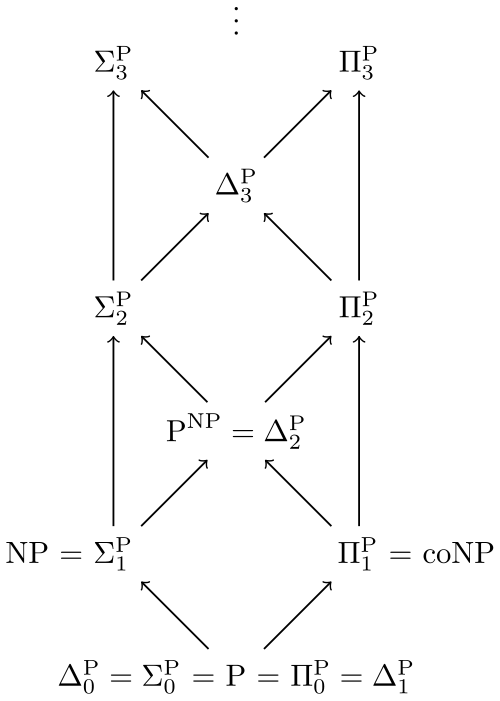
\includegraphics[width=0.3\textwidth]{img/ph_diagram.png}
  \caption{Polynomial hierarchy diagram \label{fig:ph_diagram}}
\end{figure}

\subsection{$\bPSPACE$}
In this work, I consider yet another complexity class called $\bPSPACE$ that
concerns the complexity of space.
It consists of problems that can be decided in polynomial space.

\begin{definition}
	The class $\bPSPACE$ is the class of decision problems solvable by a TM
	in space polynomial in the size of the input.
\end{definition}
It is not hard to see the following relation hold.
\begin{center}
	$\bPH \subseteq \bPSPACE$.
\end{center}

I illustrate the relationship among the complexity classes in
\figref{comp_diagram}. Many classes are omitted in our diagram
that are not in our focus.

\begin{figure}[h!]
  \centering
  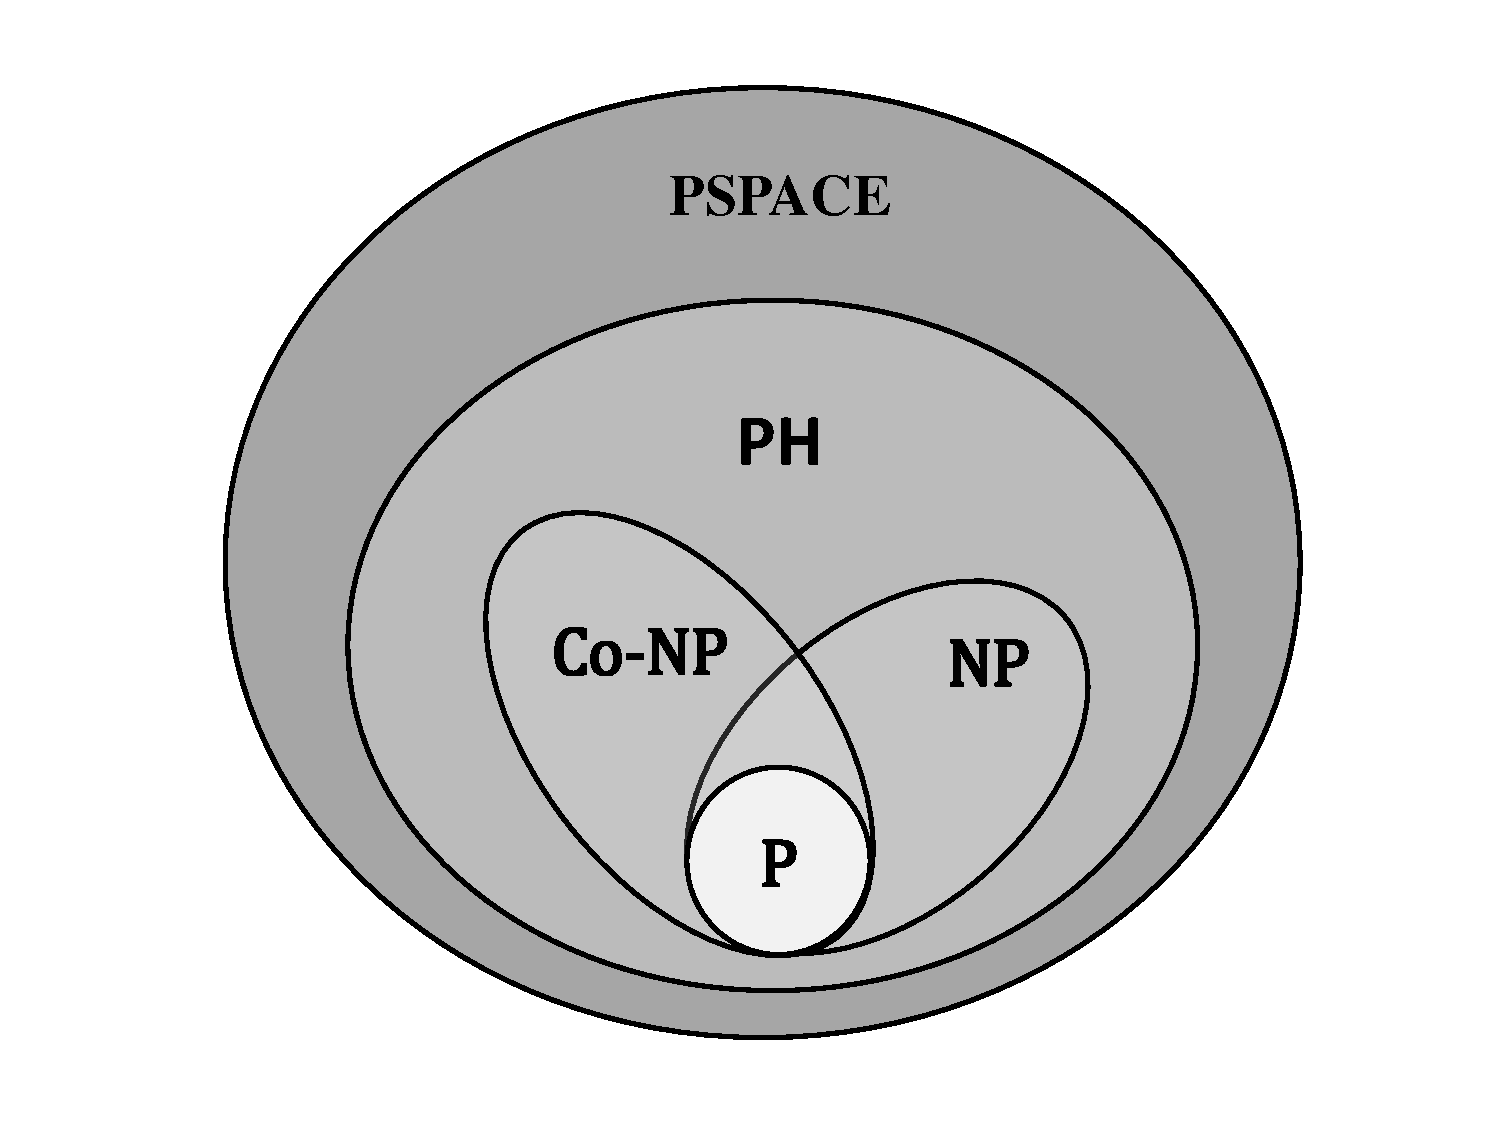
\includegraphics[width=0.7\textwidth]{img/comp_diagram.pdf}
  \caption{Computational complexity diagram \label{fig:comp_diagram}}
\end{figure}



%Note the copyright notice at the end of each chapter.
\copyrightnotice

\chapter{Related Work\label{ch:relwork}}
%%%%%%%%%% Related work
\nop{\tc{
	I will discuss what other people have done regarding
	the problems in Introduction: 
	what formalisms of preferences have been
	introduced, what solutions have been proposed to solve
	these problems.
}}

In this section I will present work related to my thesis research.
I will first review some of the preference
systems studied in the literature that are designed to represent
qualitative preferences over combinatorial domains. 
I will then introduce concepts
from social choice theory underlying methods to
combine individual preferences to reach a common decision.

\section{Preferences Modeling and Reasoning \label{sec:pref_reasoning}}
Researchers have proposed several languages to model preferences.
I will now discuss those of them that are closely related
to my work.
These languages include graphical formalisms:
\tit{Conditional Preference Networks} (CP-nets) and
\tit{Lexicographic Preference Trees} (LP-trees);
and logical formalisms:
\tit{Possibilistic Logic} and
\tit{Answer Set Optimization} (ASO).
They are developed to provide concise and intuitive
presentations of preferential information for objects from
combinatorial domains.

For all systems, I will focus on two aspects:
the language in which preferences are specified,
and complexity of and algorithms for
problems about the model.
The most fundamental of these problems are introduced
in the following definitions.

\nop{{\bf [THESE DEFINITIONS ARE AT A WRONG PLACE.]}}
\begin{definition}
\label{def:con}
  $\cL$-CONSISTENCE: given an instance $\cC$ of a preference
	formalism $\cL$, decide whether $\cC$ is consistent, that is,
  whether there exists a total order of outcomes that agrees with every
	preference statement in $\cC$.
\end{definition}

\begin{definition}
\label{def:dom}
  $\cL$-DOMINANCE: given an instance $\cC$ of a preference
	formalism $\cL$ and its two distinct outcomes
  $o_1$ and $o_2$, decide whether $o_1 \succ_\cL o_2$, that is,
  whether $o_1$ is strictly preferred to $o_2$ in $\cC$.
\end{definition}

\begin{definition}
\label{def:opt1}
  $\cL$-OPTIMALITY-\rom{1}: given an instance $\cC$ of a preference
	formalism $\cL$,
  decide whether $\cC$ has an optimal outcome.
\end{definition}

\begin{definition}
\label{def:opt2}
  $\cL$-OPTIMALITY-\rom{2}: given an instance $\cC$ of a preference
	formalism $\cL$ and an outcome $o$ of $\cC$,
  decide whether $o$ is an optimal outcome.
\end{definition}

\begin{definition}
\label{def:opt3}
  $\cL$-OPTIMALITY-\rom{3}: given an instance $\cC$ of a preference
	formalism $\cL$ and some property $\Phi$ expressed as a Boolean formula 
	over the alphabet of $\cC$,
  decide whether there is an optimal outcome $o$ that satisfies $\Phi$.
\end{definition}

\subsection{Conditional Preference Networks}
\noindent{\textbf{The Language.}}
Conditional Preference Networks (CP-nets) define preferential relations between outcomes
based on the \tit{ceteris paribus}
semantics \cite{bbdh03}.
\textit{Ceteris paribus} is latin for ``everything else being equal."

Let $\bV$ be a set of binary variables\footnote{
	Focusing on binary variables makes the discussion clearer,
	and it does not affect the complexity results.
}
, we denote by $\Asst(\bV)$ the set of
all truth assignments to the variables in $\bV$.
For each variable $X_i \in \bV$, $\Pa(X_i)$ denotes the \tit{parent} variables of
$X_i$, such that preferences over the domain of $X_i$ depend upon how
$\Pa(X_i)$ are evaluated.
%\begin{definition}
%\label{def:pi}
%	A set of variables $\bX$ is \tit{preferentially independent}
%	of $\bY=\bV-\bX$ if $\forall \bx_1,\bx_2 \in \Asst(\bX)$ and
%	$\forall \by_1,\by_2 \in \Asst(\bY)$,
%	\begin{center}
%		$\bx_1\by_1 \succeq \bx_2\by_1 \; \itiff \; \bx_1\by_2 \succeq \bx_2\by_2$.
%	\end{center}
%\end{definition}
%
%\begin{definition}
%\label{def:cpi}
%	Let $\bX$, $\bY$ and $\bZ$ be nonempty sets such that
%	$\bX \cup \bY \cup \bZ = \bV$.
%	$\bX$ is conditionally preferentially independent
%	of $\bY$ given an assignment $\bz$ to $\bZ$ 
%	if $\forall \bx_1,\bx_2 \in \Asst(\bX)$ and
%	$\forall \by_1,\by_2 \in \Asst(\bY)$,
%	\begin{center}
%		$\bx_1\by_1\bz \succeq \bx_2\by_1\bz \; \itiff \; \bx_1\by_2\bz \succeq \bx_2\by_2\bz$.
%	\end{center}
%\end{definition}
%
%\begin{definition}
%	For each variable $X_i$, $\Pa(X_i)$ denotes its parent variables such that,
%	given an assignment to $\Pa(X_i)$, $X_i$ is conditionally preferentially independent
%	of $\bV-(\Pa(X_i) \cup \{X_i\})$.
%\end{definition}

\begin{definition}
\label{def:cpn}
	Let $\bV$ be a set of binary variables $\bV=\{X_1,\ldots,X_n\}$.
	A CP-net over $\bV$ is a tuple ($G$,$T$), where
	\begin{enumerate} \itemsep -4pt
		\item $G$ is a directed graph ($V,E$) specifying
					dependencies among variables,
					where for every $X_i \in V$ we have
					$\Pa(X_i)=\{X_j:(X_j,X_i) \in E\}$,
		\item $T$ is a collection of 
					conditional preference tables (CPTs) for
					all variables.  A $\CPT(X_i)$ consists of preference
					statements of the form
					\begin{center}
						$\bu : \succ^i_{\bu}$,
					\end{center}
					where $\bu \in \Asst(\Pa(X_i))$ and $\succ^i_{\bu}$
					is a total order over $\Dom(X_i)$ given $u$.
	\end{enumerate}
\end{definition}

\nop{\mc{Need an example of CP-net here.}}
We say that a CP-net $N=(G,T)$ is \tit{acyclic} if
$G$ is acyclic; \tit{cyclic}, otherwise.
To illustrate, let us consider the domain of cars.
For simplicity, we take three binary variables
\tit{Price}, \tit{Safety}, and \tit{Capacity}.
Variable \tit{Capacity} ($C$) has two values \tit{high} ($c$) 
and \tit{low} ($\bar{c}$).
Variable \tit{Price} ($P$) has two values \tit{high} ($p$) 
and \tit{low} ($\bar{p}$).
Variable \tit{Safety} ($S$) has two values \tit{high} ($s$) 
and \tit{low} ($\bar{s}$).
An example CP-net $N=(G,T)$ over binary variables $\bV=\{C,P,S\}$
is shown in \figref{CPN_depend}.
The directed graph $G$, also called the \tit{dependency graph}, expresses
dependencies among variables.  An arrow in the dependency graph points
to a child variable from a parent variable. Thus, we see that,
the preferences on \tit{Price} (\tit{Safety}) depend upon the assignment made
to \tit{Capacity} (\tit{Price}, respectively).

\nop{\noindent{\textbf{The Model.}}}
To decide if outcome $o_1$ is preferred to outcome $o_2$ in a CP-net $N$,
one needs to show that $o_2$ can be improved, ceteris paribus, 
according to the preference statements in $N$ to reach $o_1$.

\begin{definition}
	Let $N$ be a CP-net over $\bV$, $X_i \in \bV$, $\bU = \Pa(X_i)$,
	and $\bY=\bV-(\bU \cup \{X_i\})$.
	Let $\bu x_i \by$ be an outcome, where $x_i\in \Dom(X_i)$,
	$\bu \in \Asst(\bU)$, and $\by \in \Asst(\bY)$.
	An \tit{improving flip} of $\bu x_i \by$ wrt $X_i$ is an
	outcome $\bu x_i' \by$ such that $x_i' \succ^i_{\bu} x_i$.
	A \tit{sequence of improving flips} wrt $N$ is a sequence of
	outcomes $o_1,\ldots,o_j$ such that, for every $k<j$,
	$o_{k+1}$ is an improving flip of $o_k$ wrt some variable in $\bV$.
	We say that outcome $o_1$ is preferred to outcome $o_2$ in $N$,
	denoted by $o_1 \succ_N o_2$, if there exists a sequence of
	improving flips from $o_2$ to $o_1$.
\end{definition}

In a CP-net $N$, we say that outcome $o$ is \tit{optimal} if
there does not exist another outcome $o'$ such that
$o' \succ_N o$.

%\begin{definition}
%	Let $N$ be a CP-net over $\bV$, $X_i \in \bV$, and $\bU = \Pa(X_i)$.
%	Given an assignment $\bu$ to $\bU$,
%	a total order $\succ$ over $\Asst(\bV)$ \textit{satisfies}
%	$\succ^i_{\bu}$ if for all $\by \in \Asst(\bY)$ and all
%	$x,x' \in \Dom(X_i)$, $\bu \it{x} \by \succ \bu \it{x'} \by$ whenever
%	$x \succ^i_{\bu} x'$.
%	$\succ$ \textit{satisfies}
%	$\CPT(X_i)$ if it satisfies $\succ^i_{\bu}$ for each
%	$\bu \in \Asst(\bU)$.
%	$\succ$ \textit{satisfies}
%	the CP-net $N$ if it satisfies $\CPT(X_i)$ for every $X_i$.
%	A CP-net $N$ is \textit{consistent} $\itiff$ there exists a total order
%	$\succ$ that satisfies $N$.
%\end{definition}

Consider the CP-net $N$ in \figref{CPN}.
It induces a partial order shown in \figref{CPN_pref},
where each arrow represents an improving flip between two outcomes.
We see that $c\bar{p}\bar{s} \succ_N \bar{c}ps$
because of the improving flipping sequence --
$c\bar{p}\bar{s},\bar{c}\bar{p}\bar{s},\bar{c}\bar{p}s,\bar{c}ps$.
Outcome $cps$ is optimal because no other outcome is
better.
We note that there is no flipping sequence between
$c\bar{p}s$ and $\bar{c}\bar{p}\bar{s}$.
In such case, we say that the two outcomes are \tit{incomparable}.
This CP-net is consistent because there exists a total order
of outcomes that agrees with the preference graph \figref{CPN_pref}.
There are in fact two such total orders:

\begin{center}
	$cps \succ cp\bar{s} \succ c\bar{p}\bar{s} 
		\succ \bm{c\bar{p}s} \succ \bm{\bar{c}\bar{p}\bar{s}} 
		\succ \bar{c}\bar{p}s \succ \bar{c}ps \succ \bar{c}p\bar{s}$,\\
	$cps \succ cp\bar{s} \succ c\bar{p}\bar{s} 
		\succ \bm{\bar{c}\bar{p}\bar{s}} \succ \bm{c\bar{p}s}
		\succ \bar{c}\bar{p}s \succ \bar{c}ps \succ \bar{c}p\bar{s}$.
\end{center}

%\begin{figure}[h!]
%  \centering
%  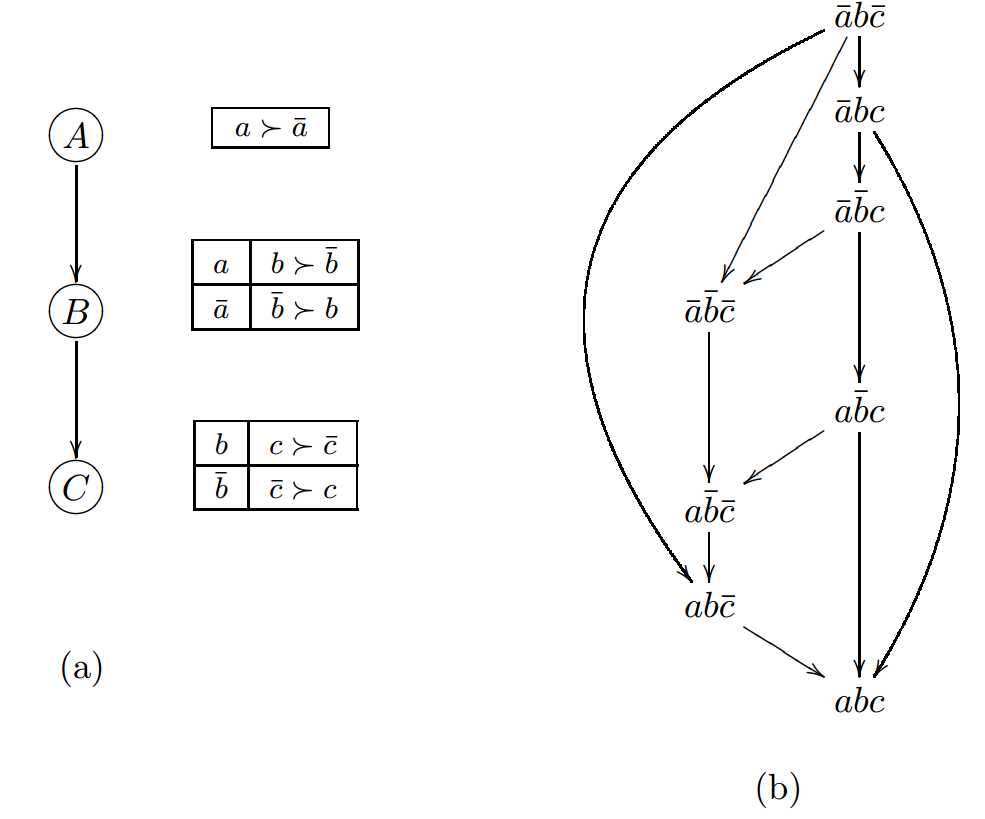
\includegraphics[width=0.7\textwidth]{img/acpn.png}
%  \caption{Acyclic CP-net \label{fig:cp_net}}
%\end{figure}

\begin{figure}[!ht]
	\centering
  \begin{subfigure}[b]{0.45\textwidth}
		\centering
	  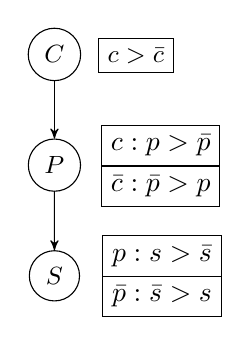
\begin{tikzpicture}[->,>=stealth',
	    level/.style={sibling distance=2cm/#1, level distance=40pt}]
	    \node [main node] (1){$C$}
	      child {node [main node] (2) {$P$}
	      	child {node [main node] (3) {$S$} {}
							child {node [rectangle,draw] (4) at (1.7,4.2) {$c>\bar{c}$} edge from parent[draw=none]}
							child {node [rectangle split, rectangle split parts=2,draw] (5) at (1.35,2.8)
								{$c:p>\bar{p}$ \nodepart{second} $\bar{c}:\bar{p}>p$} edge from parent[draw=none]}
							child {node [rectangle split, rectangle split parts=2,draw] (6) at (0.7,1.4) 
								{$p:s>\bar{s}$ \nodepart{second} $\bar{p}:\bar{s}>s$} edge from parent[draw=none]}
					}
	      };
	  \end{tikzpicture}
		\caption{Dependency graph and CPT's\label{fig:CPN_depend}}
	\end{subfigure}%
  \begin{subfigure}[b]{0.45\textwidth}
		\centering
		  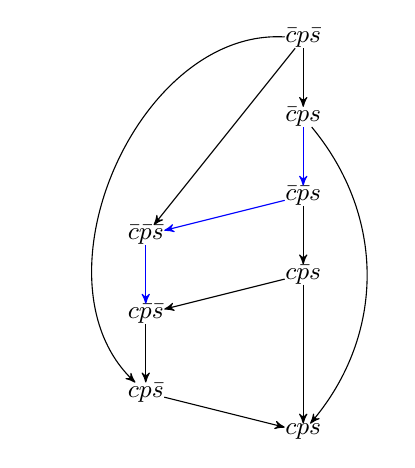
\begin{tikzpicture}[->,>=stealth',node distance=1cm,main node/.style={circle,draw,font=\small}]
		    \node[rectangle,inner sep=0pt] (1)                                         {$\bar{c}p\bar{s}$};
				\node[rectangle,inner sep=0pt] (2) [below of=1]                            {$\bar{c}ps$};
				\node[rectangle,inner sep=0pt] (3) [below of=2]                            {$\bar{c}\bar{p}s$};
				\node[rectangle,inner sep=0pt] (4) [left of =3,xshift=-1cm,yshift=-0.5cm]  {$\bar{c}\bar{p}\bar{s}$};
				\node[rectangle,inner sep=0pt] (5) [below of=3]                            {$c\bar{p}s$};
				\node[rectangle,inner sep=0pt] (6) [left of=5,xshift=-1cm,yshift=-0.5cm]   {$c\bar{p}\bar{s}$};
				\node[rectangle,inner sep=0pt] (7) [below of=6]                            {$cp\bar{s}$};
				\node[rectangle,inner sep=0pt] (8) [below of=5,yshift=-1cm]                {$cps$};
		
		    \path[every node/.style={font=\sffamily\small}]
		      (1) edge (2)
		      (1) edge (4)
		      (1) edge [bend right=70] (7)
		      (2) edge[blue] (3)
		      (2) edge [bend left=40] (8)
		      (3) edge[blue] (4)
		      (3) edge (5)
		      (4) edge[blue] (6)
		      (5) edge (6)
		      (5) edge (8)
		      (6) edge (7)
		      (7) edge (8);
		  \end{tikzpicture}
		\caption{Preference graph\label{fig:CPN_pref}}
	\end{subfigure}
  \caption{Acyclic CP-net}
  \label{fig:CPN}
\end{figure}

%Answering the CP-CONSISTENCE problem depends upon whether
%its dependency graph are acyclic and how preference rules
%in CPTs are specified.
%Researchers in AI have been working on this problem
%and many results can be found in the literature.



\noindent{\textbf{Problems and Complexity.}}
Boutilier, Brafman, Domshlak, Hoos and Poole \cite{bbdh03} 
have proved that every acyclic CP-net
is consistent, whereas Goldsmith, Lang, Truszczynski and Wilson \cite{Goldsmith}
have shown that the CPN-CONSISTENCE problem is PSPACE-complete in general.

For the CPN-DOMINANCE problem, its complexity depends on the structure
of the dependency graph.
The CPN-DOMINANCE problem can be solved by
a polynomial time algorithm for binary-valued tree-structured
CP-nets, and that the problem is NP-complete for binary-valued
CP-nets with specially structured dependency graphs 
(e.g., max-$\delta$-connected dependency graphs) \cite{bbdh03}.
However, it is NP-hard for general binary-valued acyclic 
CP-nets \cite{bbdh03}.
Furthermore, in the most general case when the dependency graph
could be cyclic, this problem is PSPACE-complete even
if the CP-nets are consistent \cite{Goldsmith}.

For acyclic CP-nets, the optimality problems (i.e.,
CPN-OPTIMALITY-\rom{1}, CPN-OPTIMALITY-\rom{2}, and
CPN-OPTIMALITY-\rom{3}) are easy \cite{bbdh03}.



\subsection{Lexicographic Preference Trees \label{sec:LPT}}
The language of lexicographic preference trees \cite{booth:learningLP} 
uses trees to model preferences. It is motivated by lexicographic
orderings \cite{Kaci:Pref} and lexicographic preferences \cite{10.2307/2296854}.
This formalism and its variants are the primary focus on my research.

\noindent{\textbf{The Language.}}
\tit{A lexicographic preference tree} (\emph{LP-tree}) $T$ over a set $\cI$ 
of $p$ binary attributes $X_1,\ldots,X_p$ is a labeled \emph{binary tree}. Each
node $t$ in $T$ is labeled by an attribute from $\cI$, denoted by 
$\mathit{Iss}(t)$, and with \emph{preference information} of the form
$a>b$ or $b>a$ indicating which of the two values $a$ and $b$  comprising
the domain of $\Iss(t)$ is preferred (in general the preference may depend
on the values of attributes labeling the ancestor nodes). We require that 
each attribute appears exactly once on each path from the root to a leaf. 

Intuitively, the attribute labeling the root of an LP-tree is of highest 
importance. Alternatives with the preferred value of that attribute
are preferred over outcomes with the non-preferred one. The two
subtrees refine that ordering. The left subtree determines the ranking
of the preferred ``upper half'' and the right subtree determines the 
ranking of the non-preferred ``lower half.'' In each case, the same 
principle is used, with the root attribute being the most important one. 
\nop{The attribute labeling the root of a subtree is the
most important among those appearing in the subtree, and the outcomes
the subtree represents are split into the preferred and non-preferred 
halves based on their value and on the preference information at the node.}
We note that the attributes labeling the roots of the 
subtrees need not be the same (the relative importance of attributes may 
depend on values for the attributes labeling the nodes on the path to the root).

The precise semantics of an LP-tree $T$ captures this intuition. Given 
an outcome $x_1x_2\ldots x_p$, we find its preference ranking in 
$T$ by traversing the tree from the root to a leaf. When at node $t$ 
labeled with the attribute $X_i$, we follow down to the left subtree if
$x_i$ is preferred according to the preference information at node
$t$. Otherwise, we follow down to the right subtree. 

It is convenient to imagine the existence of yet another level of nodes 
in the tree, not represented explicitly, with each node in the lowest 
level ``splitting'' into two of these
implicit nodes, each representing an outcome. Descending the tree 
given an outcome in the way described above takes us to an (implicit) 
node that represents precisely that outcome's rank.
The more to the left the node representing the outcome, the more 
preferred it is, with the one in the leftmost (implicit) node being the 
most desirable one as left links always correspond to preferred values.

To illustrate these notions, let us consider an example LP-tree
over the car domain, given by the three binary attributes 
\tit{Capacity}, \tit{Price}, and \tit{Safety},
described as earlier.
Our agent prefers cars with high capacity to cars with low capacity,
and this preference on \tit{Capacity} is the most important one.
Then, for high-capacity cars, the next most important attribute is
\tit{Safety} and she prefers cars with high security level,
and the least important attribute is \tit{Price}.
She prefers low-price cars if security is low, and high-price, otherwise.
For low-capacity cars, the importance of \tit{Safety}
and \tit{Price} changes with \tit{Price} being more important.
The agent prefers low-price cars among the low-capacity.
Finally, high-security cars are preferred over low-security cars.
These preferences are captured by 
the LP-tree $T$ in Figure \ref{fig:LPTree_full}. The tree shows that
the most preferred car for our agent has high capacity, security,
and price, and the next in order of preference has high capacity
and security but low price.

\begin{figure}
  \small
	\centering
	\hspace{-1cm}
	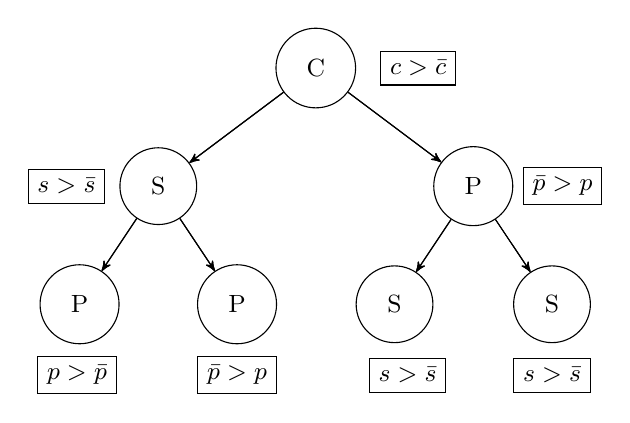
\begin{tikzpicture}[->,>=stealth',
	  level/.style={sibling distance=4cm/#1}]
	  \node [main node,inner sep=7pt] (1){C}
	    child {node [main node,inner sep=7pt] (2) {S}
	      child {node [main node,inner sep=7pt] (3) {P}}
	      child {node [main node,inner sep=7pt] (4) {P}
					child {node [rectangle,draw] at (6.3,4.5) {$c>\bar{c}$} edge from parent[draw=none]}
					child {node [rectangle,draw] at (0.5,3) {$s>\bar{s}$} edge from parent[draw=none]}
					child {node [rectangle,draw] at (-0.7,0.6) {$p>\bar{p}$} edge from parent[draw=none]}
					child {node [rectangle,draw] at (0,0.6) {$\bar{p}>p$} edge from parent[draw=none]}
					child {node [rectangle,draw] at (2.8,3) {$\bar{p}>p$} edge from parent[draw=none]}
					child {node [rectangle,draw] at (-0.5,0.6) {$s>\bar{s}$} edge from parent[draw=none]}
					child {node [rectangle,draw] at (0,0.6) {$s>\bar{s}$} edge from parent[draw=none]}
				}
	    }
	    child {node [main node,inner sep=7pt] (5) {P}
	    child {node [main node,inner sep=7pt] (6) {S}}
	      child {node [main node,inner sep=7pt] (7) {S}}
	    };
	    \path[every node/.style={font=\sffamily\small}]
	      (1) edge (2)
	          edge (5)
	      (2) edge (3)
	          edge (4)
	      (5) edge (6)
	      		edge (7);
	\end{tikzpicture}
   
  \caption{An LP-tree $T$}
  \label{fig:LPTree_full}
\end{figure}

Sometimes LP-trees can be represented in a more concise way. For 
instance, if for some node $t$, its two subtrees are identical (that 
is, the corresponding nodes are assigned the same attribute), they can be 
collapsed to a single subtree, with the same assignment of attributes to 
nodes. To retain preference information, at each node $t'$ of the 
subtree we place a \emph{conditional preference table},
and each preference in it specifies 
the preferred value for the attribute labeling that node given the value 
of the attribute labeling $t$. In the extreme case when for every node its
two subtrees are identical, the tree can be collapsed to a path. 

%Since the preferred attribute at a node depends on the values of attributes above,
%the conditional preference table for the node $t$ located at distance 
%$i$ from the root has possibly as many as $2^i$ rows (in general, 
%$2^j$ rows, where $j$ is the number of ancestor nodes with one child 
%only), with each row specifying a combination of values for the ancestor 
%attributes together with the preferred value for $\Iss(t)$ given that 
%combination. Thus, collapsing subtrees alone does not lead to a smaller 
%representation size. However, it can be achieved if there are nodes whose 
%preferred value depends only on a limited number of attributes labeling 
%their single-child ancestor nodes as in such cases the conditional 
%preference table can be simplified.  

Formally, given an LP-tree (possibly with some subtrees collapsed), for 
a node $t$, let $\ninst(t)$ be the set of ancestor nodes of $t$ whose
subtrees were collapsed into one, and let $\Inst(t)$ represent the 
remaining ancestor nodes. A \emph{parent} function $\cP$ assigns to 
each node $t$ in $T$ a set $\cP(t)\subseteq\ninst(t)$ of \emph{parents}
of $t$, that is, the nodes whose attributes may have influence on the local 
preference at $\Iss(t)$. Clearly, the conditional preference table at $t$
requires only $2^{|\cP(t)|}$ rows, possibly many fewer than in the worst 
case. In the extreme case, when an LP-tree is a path and each node has 
a bounded (independent of $p$) number of parents, the tree can be 
represented in $O(p)$ space.

If for every node $t$ in an LP-tree, $\cP(t)=\emptyset$, all (local)
preferences are unconditional and conditional preference tables consist
of a single entry. Such trees are called \emph{unconditional preference}
LP-trees (UP trees, for short). Similarly, LP-trees with all non-leaf 
nodes having their subtrees collapsed are called an \emph{unconditional
importance} LP-trees (UI trees, for short). This leads to a a natural 
classification of LP-trees into four classes: unconditional importance 
and unconditional preference LP-trees (UI-IP trees), unconditional 
importance and conditional preference trees (UI-CP trees), etc. The class
of CI-CP trees comprises all LP-trees, the class of UI-UP trees is the 
most narrow one. 

The LP-tree $T$ in Figure \ref{fig:LPTree_full} can be represented more
concisely as a (collapsed) CI-CP tree $v$ in Figure \ref{fig:LPTree}. Nodes
at depth one have their subtrees collapsed. In the tree in Figure
\ref{fig:LPTree_full}, the subtrees of the node at depth 1 labeled 
\tit{P} are not only identical but also have the same preference 
information at every node. Thus, collapsing them does not incur growth in
the size of the conditional preference table.
      
\begin{figure}
   \small
	\centering

  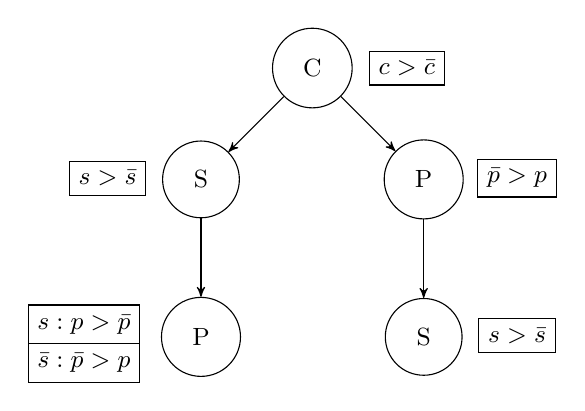
\begin{tikzpicture}[->,>=stealth',node distance=2cm,main node/.style={circle,draw,font=\small}]
        
    \node[main node,inner sep=7pt] (1) {C};
    \node[rectangle,draw] at (1.2,0) {$c > \bar{c}$};
    
    \node[main node,inner sep=7pt] (2) [below left of=1] {S};
    \node[rectangle,draw] at (-2.6,-1.4) {$s>\bar{s}$};
		%\node[rectangle] at (-2.0,-1.4) {$t'$};
    
    \node[main node,inner sep=7pt] (3) [below of=2] {P};
    \node[rectangle split, rectangle split parts=2, draw, font=\sffamily\small] at (-2.9,-3.5)
        {
          $s:p>\bar{p}$
          \nodepart{second}
          $\bar{s}:\bar{p}>p$
        };
    %\node[rectangle] at (-2,-3.5) {$t$};
    
    \node[main node,inner sep=7pt] (4) [below right of=1] {P};
    \node[rectangle,draw] at (2.6,-1.4) {$\bar{p} > p$};
    
    \node[main node,inner sep=7pt] (5) [below of=4] {S};
    \node[rectangle,draw] at (2.6,-3.4) {$s > \bar{s}$};
  
    \path[every node/.style={font=\sffamily\small}]
      (1) edge (2)
          edge (4)
      (2) edge (3)
      (4) edge (5);
  \end{tikzpicture}
  
%  \vspace{-0.3cm}
  \caption{A CI-CP LP-tree $T$}
  \label{fig:LPTree}
%  \vspace{-0.5cm}
\end{figure}

\nop{\noindent{\textbf{The Model.}}}
An LP-tree consisting of $p$ binary attributes corresponds to a total order over
$2^p$ outcomes.  For the example in \figref{LPTree}, the total order induced
by $T$ is
\begin{center}
	$cps \succ c\bar{p}s \succ c\bar{p}\bar{s} \succ cp\bar{s} 
		\succ \bar{c}\bar{p}s \succ \bar{c}\bar{p}\bar{s} \succ \bar{c}ps \succ \bar{c}p\bar{s}$.
\end{center}

\noindent{\textbf{Problems and Complexity.}}
As any LP-tree induces a total order, the $\LP$-CONSISTENCE problem is trivial.
Moreover, an optimal outcome always exists and the $\LP$-OPTIMALITY-\rom{1} problem
is trivial too.  Similarly, the $\LP$-OPTIMALITY-\rom{2} and
$\LP$-OPTIMALITY-\rom{3} problems are easy to solve.
Deciding whether outcome $o_1$ dominates outcome $o_2$ is done by traversing the tree
and check the attributes accordingly until an attribute $X$ is reached such that
$o_1(X) \not = o_2(X)$.  Alternatives $o_1$ and $o_2$ are then ordered based on the preference
information on $X$ \cite{booth:learningLP}.
Therefore, we know that the $\LP$-DOMINANCE problem is in \bP.

%\begin{thm}
%\label{thm:LP_DOM}
%	The $\LP$-DOMINANCE problem can be solved in time linear in $p$.
%\end{thm}
%\begin{proof}
%	The linear time algorithm is shown in \algref{LP_dom}.
%
%	\begin{algorithm}[ht]
%	\KwIn{an LP-tree $T$, two outcomes $o_1$ and $o_2$ ($o_1 \not = o_2$)}
%	\KwOut{$\true$ if $o_2 \succ_T o_1$; $\false$, otherwise}
%	Let $T^* = T$\;
%	\For{$i \leftarrow 1$ \KwTo $p$}{
%	  Let $X_j$ be the root of $T^*$ with preference $x_j \succ \bar{x_j}$\;
%	  
%	  \uIf{$o_2(X_j) > o_1(X_j)$}{
%			\Return{$\true$}\;
%	  }
%		\uElseIf{$o_2(X_j) < o_1(X_j)$}
%		{
%			\Return{$\false$}\;
%	  }
%		\Else{
%			$T^* \leftarrow T^*(x_j)$\;
%		}
%	}
%	
%	\caption{Solving the $\LP$-DOMINANCE problem\label{alg:LP_dom}}
%	\end{algorithm}
%\end{proof}

In addition to problems of reasoning about a single
LP-tree, recently researchers have initiated studies of
the problem of aggregating LP-trees expressing preferences of multiple
agents. The goal is to facilitate collaborative decision making.
LP-trees are aggregated
according to some social choice scheme, such as
issue-by-issue voting \cite{fargier:ibi},
sequential majority voting rule \cite{Xia:SMV},
positional scoring rules (e.g. Borda, $k$-Approval) \cite{lang,LiuT}.
Basics of social choice are discussed later in this chapter.
In \chref{aggLP}, I will provide detailed definitions of aggregating
problems and results I obtained on their complexity 
according to positional scoring rules, as
well as experimental analysis for two computational tools:
Answer Set Programming (ASP) \cite{aspataglance} and 
Weighted Partial Maximum Satisfiability (WPM) \cite{papado:b:compcomplexity}.


\subsection{Possibilistic Logic}
Unlike CP-nets and LP-trees that respectively express partial orders and total orders,
possibilistic logic \cite{DuboisLP91} describes preferences as a set of weighted propositional
formulas inducing total preorders.

\noindent{\textbf{The Language and the Model.}}
In possibilistic logic, preferences are stated as a theory of weighted formulas.
A possibilistic logic theory $\Pi$ over a vocabulary $\cI$ is a set of 
\emph{preference pairs}
\begin{center}
	$\{ (\phi_1,a_1), \ldots, (\phi_m,a_m) \}$,
\end{center}
where every $\phi_i$ is a Boolean formula over $\cI$, and every $a_i$ is a real number
such that $1\geq a_1>\ldots>a_m\geq 0$ (if two formulas have the same 
importance level, they can be replaced by their conjunction).
Intuitively, $a_i$ represents the importance of $\phi_i$, with larger values
indicating higher importance.

The \textit{tolerance degree} of an outcome $o$ with regard to a preference 
pair $(\phi,a)$, $\TD_{(\phi,a)}(o)$, is defined by
\[
 \TD_{(\phi,a)}(o) =
  \begin{cases}
   1, & o \models \phi \\
   1-a, & o \not \models \phi
  \end{cases}
\]
Based on that, the tolerance degree of an outcome $o$ with regard to a \emph{set}
$\Pi$ of preference pairs, $\TD_\Pi(o)$, is defined by 
\begin{center}
	$\TD_\Pi(o)=min\{\TD_{(\phi_i,a_i)}(o):1\leq i \leq m\}$.
\end{center}
The larger $\TD_\Pi(o)$, the more preferred $o$ is; that is, 
given two outcomes $o_1$ and $o_2$, we have
\begin{center}
	$o_1 \succ_\Pi o_2$ \itiff $\TD_\Pi(o_1) > \TD_\Pi(o_2)$,\\
	$o_1 \approx_\Pi o_2$ \itiff $\TD_\Pi(o_1) = \TD_\Pi(o_2)$.
\end{center}

{\bf [NEED EXAMPLE]}


\subsection{Answer Set Optimization}
The formalism of Answer Set Optimization (ASO) was originally introduced by
Brewka, Nieml\"a and Truszczynski \cite{Brewka03answerset} and
later enhanced by Brewka \cite{Brewka04}.
%A declarative planning language, $\cPP$, was introduced \cite{Son:plan_pref}
%and shown that any preference in $\cPP$ can be embedded in ASO preferences
%\cite{Brewka04}.

In this work, we focus on the original framework \cite{Brewka03answerset} where 
the Pareto method is used to order outcomes.
Other methods can be found in the latter paper \cite{Brewka04}.
In more recent works \cite{Faber:QOP,Faber:APF}, 
the Pareto-based ASO framework is generalized in the setting of
qualitative optimization problems.

\noindent{\textbf{The Language.}}
\begin{definition}
	Let $A$ be a finite set of atoms.
	An ASO theory over $A$ is a tuple $(P_{\gen},P_{\PREF})$, where
	\begin{enumerate} \itemsep -4pt
		\item $P_{\gen}$, the generating program, is a logic program
					with hard constraints, built of atoms in $A$,
					used to generate answer sets called feasible outcomes,
		\item $P_{\PREF}$, the selecting program, is a preference
					program consisting of preference rules of the form
			\begin{center}
				$\gamma_1 > \ldots > \gamma_k \leftarrow \alpha$,
			\end{center}
					where each $\gamma_i$ is a propositional formula
					over $A$ and $\alpha$ is a conjunction of
					literals of atoms in $A$.
	\end{enumerate}
\end{definition}

\nop{\mc{
	Need to show an example of ASO here.
}}

\nop{\noindent{\textbf{The Model.}}}
A single ASO preference rule specifies a total preorder over outcomes.
Applying the Pareto method, a general ASO program with multiple ASO rules
describes a partial preorder over the space of outcomes represented by answer sets.

We say outcome $o$ is \tit{irrelevant} to preference rule $r$ if
$o \models (\neg \alpha) \vee (\neg \gamma_1 \wedge \ldots \wedge \gamma_k)$;
that is, if $o$ does not satisfy $\alpha$ or $o$ does not satisfy any of
the Boolean combinations. As mentioned in the work by Brewka et al \cite{Brewka03answerset},
outcomes irrelevant to $r$ are considered as good as the
best outcomes.
This default treatment of irrelevance can be overwritten by
including formula $(\neg \alpha) \vee (\neg \gamma_1 \wedge \ldots \wedge \gamma_k)$
in any place of the preference rule $r$.
Formally we define satisfaction degree of an answer set with respect to a
preference rule.
\begin{definition}
	Let $o$ be an outcome generated by $P_{\gen}$,
	$r$ an ASO preference rule.
	The satisfaction degree of $o$ on $r$, denoted $d_r(o)$,
	is defined as follows: $d_r(o)=1$ if $o$ is irrelevant to $r$;
	$d_r(o)=\min\{i:o \models \gamma_i\}$, otherwise.
\end{definition}

\begin{definition}
	Let $(P_{\gen}, P_{\PREF})$ be an ASO theory,
	$o$ and $o'$ two outcomes.
	outcome $o'$ is weakly Pareto-preferred to $o$, $o' \succeq o$,
	if, for every rule $r$ in $P_{\PREF}, d_r(o') \leq d_r(o)$.
	outcome $o'$ is strictly Pareto-preferred to $o$, $o' \succ o$,
	if $o' \succeq o$ and $o \not \succeq o'$.
	outcome $o$ is optimal if there exists no outcome $o''$ such that
	$o'' \succ o$.
\end{definition}

Consider an ASO theory $P=(P_{\gen}, P_{\PREF})$, where
\begin{center}
	$P_{\gen}=\{$
	$(a \lor \bar{a}) \land (\neg (a \land \bar{a})). \;$
	$(b \lor \bar{b}) \land (\neg (b \land \bar{b})). \;$
	$(c \lor \bar{c}) \land (\neg (c \land \bar{c})). \}$
	and\\
	$P_{\PREF}=\{
		a > \bar{a} \leftarrow b \vee c. \;\;
		b \wedge \bar{c} > \bar{b} \wedge c.
	\}$.
\end{center}
An optimal outcome is $ab\bar{c}$ and it is the only optimal one.

\noindent{\textbf{Problems and Complexity.}}
Brewka et al \cite{Brewka03answerset} proved that
the ASO-DOMINANCE problem is in P, ASO-OPTIMALITY-\rom{1}
is NP-complete, ASO-OPTIMALITY-\rom{2} is coNP-complete,
and ASO-OPTIMALITY-\rom{3} is $\sigmap{2}$-complete.

Moreover, an extended paradigm of ranked ASO programs has
been introduced in the same work \cite{Brewka03answerset}.
Ranked ASO programs are ASO programs where rules in $P_{\PREF}$
are given numeric values that represent different levels of importance
of preference rules.  Nonetheless, complexity results presented
above stay unchanged.




\section{Social Choice}
The study of preference aggregation can be traced back to social choice theory,
which dates back to Condorcet's paradox of voting, noted by the
Marquis de Condorcet in the 18th century, in which
the winning ranking of outcomes could be cyclic even 
given acyclic individual votes \cite{wiki:soc}.
Kenneth Arrow's work, \textit{Social Choice and Individual Values},
is recognized as the basis of modern social choice \cite{aarrow:b:socialchoice}.
In the book, Arrow states that any preference aggregation method for at least three
outcomes cannot meet some fairly desirable axioms, a result known as
the Arrow's impossibility theorem.
Further extending this result, Gibbard and Satterthwaite showed
that any social choice function, again meeting some fair properties, is subject
to manipulation \cite{gib:j:maip-scheme,satt:j:strat-proof}.
Extending the Gibbard-Satterthwaite theorem, the Duggan-Schwartz theorem deals with 
voting rules that elect a nonempty set of co-winners rather than a single winner
\cite{dug-sch:j:maipres}.

All these results inform us that it is impossible to design a fair preference
aggregation system that is manipulation-proof.
However, Bartholdi, Tovey and Trick proposed the idea of protecting
social choice schemes from manipulation via computational
complexity \cite{bartholdi:j:whowon,bartholdi:j:compdiff,
bartholdi:j:howhard}.
The idea is that, if manipulation is computationally hard to
achieve, manipulation is unlikely.

That started the field of computational social choice by adding an algorithmic
perspective from computer science to the formal approach 
of social choice theory \cite{Brandt:COMSOC}.




\subsection{Preference Aggregation}
One of the most fundamental problems in social choice theory is how to
aggregate individual preferences over outcomes so that a
collaborative preference relation is reached.
In other settings, people are interested in some optimal outcomes
rather than a collective preference relation over all outcomes.

\noindent{\textbf{Social Welfare Functions.}}
\begin{definition}
	Let $A=\{a_1,\ldots,a_m\}$ be a finite set of outcomes,
	$N=\{1,\ldots,n\}$ a finite set of agents (or voters).
	A preference relation (or a vote) $v_i$ given by agent $i$ 
	is a total order $\succ_i$,
	that is, a total, transitive and antisymmetric.
	A preference profile $P$ is a finite set of preference relations
	$\{\succ_1, \ldots, \succ_n\}$.
\end{definition}

We denote by $\cL(A)$ the set of all preference relations over
the space of outcomes $A$, and $\cL(A)^n$, the set of all
preference profiles.

\begin{definition}
	A social welfare function ($\SWF$) is a function $f$:
	\begin{center}
		$\cL(A)^n \rightarrow \cL(A)$.
	\end{center}
	We call the resulting relation $\succ \in \cL(A)$ the social preference relation.
\end{definition}

If there are two outcomes $a_1$ and $a_2$,
May's theorem \cite{May52} suggests that $a_1$ should be
preferred to $a_2$ in the social preference relation
if and only if more agents prefer $a_1$ to $a_2$ than
$a_2$ to $a_1$.
This idea is called the majority voting.
However, when there are more than two outcomes,
the majority voting rule can lead to cycles of
outcomes, which is known as the Condorcet's paradox.
For instance, we have three voters with the following
preference relations:
\begin{center}
	$a_1 \succ_1 a_2 \succ_1 a_3$\\
	$a_2 \succ_2 a_3 \succ_2 a_1$\\
	$a_3 \succ_3 a_1 \succ_3 a_2$
\end{center}
Based on the pairwise majority rule, we have the following cycle
\begin{center}
	$a_1 \succ a_2$, $a_2 \succ a_3$, $a_3 \succ a_1$. 
\end{center}

%A general result, Arrow's theorem, shows that no social welfare
%functions satisfies some fairness conditions, defined as follows.
%
%\begin{definition}
%	An $\SWF$ satisfies \textit{Pareto efficiency} if 
%	\begin{center}
%		$\forall i \in N, \forall a_j,a_k \in A, (a_j \succ_i a_k \Rightarrow a_j \succ a_k)$.
%	\end{center}
%	Let $N_{(a_j,a_k)}$ be the set of voters where
%	$a_j$ is preferred to $a_k$ ($N_{(a_j,a_k)}=\{i:a_j \succ_i a_k\}$).
%	An $\SWF$ satisfies \textit{independence of irrelevant outcomes} if
%	\begin{center}
%		$\forall P,P' \in \cL(A)^n, \forall a_j,a_k \in A, (N_{(a_j,a_k)}=N'_{(a_j,a_k)}\Rightarrow$\\
%		$a_j,a_k$ are ranked identically in $\succ$ and $\succ')$.
%	\end{center}
%	An $\SWF$ satisfies \textit{non-dictatorship} if there is no agent $i$ such that
%	\begin{center}
%		$\forall P \in \cL(A)^n, \forall a_j,a_k \in A, (a_j \succ_i a_k \rightarrow a_j \succ a_k)$.
%	\end{center}
%\end{definition}
%
%\begin{thm}
%\label{thm:Arrow}
%\emph{(Arrow, 1951)}
%	When there are at least three outcomes,
%	There exists no $\SWF$ that simultaneously satisfies
%	Pareto efficiency, independence of irrelevant outcomes
%	and non-dictatorship.
%\end{thm}



\noindent{\textbf{Social Choice Functions.}}
\begin{definition}
	A social choice function ($\SCF$) is a function $f$:
	\begin{center}
		$\cL(A)^n \rightarrow 2^A-\{\emptyset\}$.
	\end{center}
	We call the resulting outcome (outcomes)
	a winner (co-winners, respectively).
\end{definition}

We now discuss some of the desirable axioms of an $\SCF$ including
resolution, anonymity and neutrality.
Note that the axioms for $\SWF$ may not directly apply here.

\begin{definition}
	An $\SCF$ $f$ is resolute if it always yields a unique winning outcome, that is,
	\begin{center}
		$\forall P \in \cL(A)^n, |f(P)|=1$.
	\end{center}
	$f$ is anonymous if names of the voters do not matter, that is,
	for every permutation $\pi$ on voters,
	\begin{center}
		$f({v_1,\ldots,v_n}) = f(v_{\pi(1)},\ldots,v_{\pi(n)})$.
	\end{center}
	$f$ is neutral if names of the outcomes do not matter, that is,
	for every profile $P$ and every permutation $\pi$ on outcomes,
	\begin{center}
		$\pi(f(P)) = f(\pi(P))$.
	\end{center}
\end{definition}

Surprisingly, these three fairness conditions cannot be satisfied simultaneously
by any $\SCF$. We have the following easy impossibility theorem \cite{Brandt:COMSOC}.

\begin{thm}
\label{thm:easy}
	A resolute $\SCF$ cannot satisfy both anonymity and neutrality.
\end{thm}
%\begin{proof}
%	Consider the election with two votes over two outcomes $a$ and $b$:
%	\begin{center}
%		$P=\{a \succ_1 b, b \succ_2 a\}$.
%	\end{center}
%	We apply the resolute $\SCF$: the majority rule with tie-breaking in favor of $a$.
%	So $a$ wins in $P$.
%	Assuming anonymity, we still have $a$ as the winner in profile $P'$:
%	\begin{center}
%		$P'=\{a \succ_2 b,b \succ_1 a\}$.
%	\end{center}
%	Let us assume neutrality also holds, $b$ wins in $P'$.  Contradiction!
%
%\end{proof}

%The three axioms discussed in Arrow's theorem need adjusting 
%in the setting of social choice functions.
%Below we show how Pareto efficiency and non-dictatorship are aligned.
%
%\begin{definition}
%	An $\SCF$ $f$ satisfies \textit{Pareto efficiency} if 
%	\begin{center}
%		$\forall v_i \in P, \forall a_j,a_k \in A, (a_j \succ_i a_k \Rightarrow a_k \not \in f(P))$.
%	\end{center}
%	An $\SCF$ satisfies \textit{non-dictatorship} if there is no agent $i$ such that
%	\begin{center}
%		$\forall P \in \cL(A)^n, (a=\topFunc(v_i) \Rightarrow a \in f(P))$,
%	\end{center}
%	where $\topFunc(v_i)$ returns the top ranked outcome in vote $v_i$.
%\end{definition}
%
%\begin{definition}
%	An $\SCF$ $f$ satisfies \textit{liberalism} if 
%	for every agent $i \in N$, there are two different outcomes $a,b \in A$ such that
%	\begin{center}
%		$i \in P_{(a,b)} \Rightarrow b \not \in f(P)$ and $i \in P_{(b,a)} \Rightarrow a \not \in f(P)$.
%	\end{center}
%\end{definition}
%
%The following theorem by A. Sen \cite{Sen} states the impossibility of an $\SCF$ satisfying
%both Pareto efficiency and liberalism.
%
%\begin{thm}
%\label{thm:Sen}
%\emph{(Sen, 1971)}
%	When there are at least two agents,
%	there exists no $\SCF$ that simultaneously satisfies
%	Pareto efficiency and liberalism.
%\end{thm}

Another desirable property of an $\SCF$ is that if the support of a winning
outcome grows then it stays a winner in the new profile.
This condition is called monotonicity. Formally, we define monotonicity as follows.

\begin{definition}
	An $\SCF$ $f$ satisfies \textit{monotonicity} if 
	\begin{center}
		$\forall a,b \in A, \forall P,P' \in \cL(A)^n, (a \in f(P) \wedge 
		N_{(a,b)} \subseteq N'_{(a,b)} \Rightarrow a \in f(P'))$.
	\end{center}
\end{definition}

For instance, the majority rule (plurality) does not satisfy monotonicity, but 
the Condorcet rule does.  Another desired property is that every outcome
has a chance to win, namely, surjectivity (or non-imposingness).  More formally, 
an $\SCF$ $f$ is surjective if for every outcome $a \in A$, there exists
some profile $P$ such that $a \in f(P)$.
Regarding the aforementioned two fairness conditions, Muller and Satterthwaite \cite{Mull_Satt}
proved yet another impossibility theorem for $\SCF$'s.

\begin{thm}
\label{thm:Mull_Satt}
\emph{(Muller and Satterthwaite, 1977)}
	When there are at least three outcomes,
	any resolute $\SCF$ satisfying monotonicity and surjectivity is dictatorial.
\end{thm}



\subsection{Voting Rules}
The problem of aggregating individual preferences (or votes) into a single
collective preference relation or a single group preferred winner is
one of the key problems in social choice theory.
Several voting rules and schemas have been proposed over the years.
While, when there are three or more candidates, none of these
methods is free of some unexpected properties,
some of them have gained broad acceptance.
I will now introduce some of these commonly used voting rules.

\begin{definition}
	A voting rule $r$ is a specific $\SCF$ proposed for practical use.
\end{definition}

\noindent{\textbf{Positional Scoring Rules.}}
For profiles over a set $A$ of outcomes, 
a \emph{scoring vector} is a sequence $w= (w_1,\ldots,
w_m)$ of integers such that $w_1\geq w_2 \geq \ldots \geq w_m$
and $w_1 > w_m$. Given a vote
$v$ with the outcome $a$ in position $i$ ($1 \leq i \leq m$), 
the score of $a$ in
$v$ is given
by $s_w(v,a)=w_i$. Given a profile $P$ of votes and an outcome $a$,
the score of $a$ in $P$ is given by $s_w(P,a) = \sum_{v\in P} s_w(v,a)$. 
These scores determine the ranking generated from $P$ by the scoring
vector $w$ (assuming, as is common, some independent tie breaking rule). 
Common positional scoring rules include the plurality rule,
the veto rule, the $k$-approval rule and Borda's rule.
\begin{enumerate} \itemsep -4pt
	\item plurality: $(1,0,\ldots,0)$
	\item veto: $(1,\ldots,1,0)$
	\item $k$-approval: $(1,\ldots 1,0,\ldots 0)$ with $k$ the number of 1's
	\item Borda: $(m-1,m-2,\ldots, 1,0)$
\end{enumerate}

We propose yet another positional scoring rule, called $(k,l)$-approval \cite{LiuT},
with the scoring vector $(a,\ldots,a,b,\ldots,b,0,\ldots,0)$, where
both $a$ and $b$ are constants $(a \geq b)$ and the numbers of $a$'s and $b$'s equal to
$k$ and $l$, respectively.
Note that $(k,l)$-approval allows agents to specify two levels of approval,
compared to only one level in $k$-approval, and thus $(k,l)$-approval
generalizes $k$-approval.

A voting method, that is closely related to positional scoring rules, is
the approval voting \cite{BraFis}.
Under approval voting, each voter approves any number of outcomes
and the winner, or co-winners, are those with the highest score.

\noindent{\textbf{Condorcet Consistent Rules.}}
A \tit{Condorcet winner} is an outcome that wins every pairwise comparisons
against each of the other outcomes.
Clearly, a Condorcet winner is unique whenever it exists.
If a voting rule $r$ always selects the Condorcet winner,
if it exists, then $r$ is said to be Condorcet consistent.

Positional scoring rules are not Condorcet consistent \cite{Fis}.
Voting rules that are Condorcet consistent include the following,
only to list a few \cite{Brandt:COMSOC}.
\begin{enumerate} \itemsep -4pt
	\item Copeland's rule: An outcome scores 1 for each pairwise comparison
				it wins, and some number between 0 and 1 for each pairwise comparison
				it ties.  Alternatives with the highest score are the co-winners.
	\item Maximin: The Maximin score of an outcome $a$ is the minimum number of
				votes for $a$ among all pairwise comparisons.  
				Alternatives with the highest Maximin score wins.
	\item Kemeny's rule: It selects linear rankings that maximize the number of agreements 
				with pairwise preferences of outcomes in the profile of votes, and
				the top-ranked outcomes in these rankings are the co-winners.
	\item Dodgson's rule: A winner is an outcome that can be made a Condorcet winner 
				by a minimal number of swaps of adjacent outcomes in the votes.
\end{enumerate}

If it is required that only a single winner is eventually elected,
we apply some tie-breaking method in case of co-winners.
Such a tie-breaking method could be that we break ties in favor of
the lexicographically smallest or largest outcome, or in favor of
a randomly picked outcome among co-winners.



%\noindent{\textbf{Other Rules.}}




\subsection{Manipulation \label{sec:manip}}
In practice, preference relations, or votes, are collected from voters
who could report preferences that are not truthful.
The reason why any agent would do so is that
casting an untruthful vote, under certain circumstances,
may benefit the agent in that she could end up with
a better result, compared to the result of the election
with her true preferences.
In cases when an agent can be better off misreporting her
true preferences, we say that she can perform manipulation.
Assuming a voting rule is resolute,
we define manipulability as follows.

\begin{definition}
	A resolute voting rule $f$ is manipulable if there exist
	a voter $i \in N$ and preference profiles $P,P' \in \cL(A)^n$
	such that $P-v_i=P'-v_i'$ and $f(P) \succ_i f(P')$.
	A voting rule is strategy-proof if not manipulable.
\end{definition}

Since manipulation seems undesirable, researchers are
interested in determining what voting rules are
manipulable and what are not.
Surprisingly, as shown in the Gibbard-Satterthwaite
theorem \cite{gib:j:maip-scheme,satt:j:strat-proof},
any reasonable voting rule is susceptible to
manipulation given that the number of outcomes
is at least three.

\begin{thm}
\label{thm:Gib_Sat}
\emph{(Gibbard, 1973; Satterthwaite, 1975).}
	When there are at least three outcomes,
	every resolute, surjective, strategy-proof voting rule is
	dictatorial.
\end{thm}

Since it is impossible to have any reasonable voting rule that is strategy-proof,
researchers have worked hard to circumvent the theorem
for strategy-proof voting rules by restricting the domains
of preferences\cite{Brandt:COMSOC}.
Moulin \cite{Moul} observed that any voting rule uniquely selecting
the Condorcet winner is strategy-proof, assuming the existence
of Condorcet winners in any profile of preference relations
expressed in a restricted domain.
One such domain is the domain of single-peaked preferences
\cite{Sprumont}.

\noindent{\textbf{Computational Hardness of Manipulation.}}
In spite of the fact that voting rules can be strategy-proof
when preferences are restricted, in practice we cannot impose
constraints onto how agents should formulate their preferences.
Another approach to work around the impossibility theorem is
to protect voting rules against manipulation by showing
high computational complexity.

We first give a definition of the manipulation problem as follows.
\begin{definition}
	Let $r$ be a resolute voting rule.  Given a profile $P$ of
	$n$ votes over $m$ outcomes and an outcome $c$, 
	the manipulation problem is to decide whether there exists
	a single vote $v'$ such that $c=r(P \cup \{v'\})$.
\end{definition}

The manipulation problem is proved to be NP-hard for several
rules, such as second-order Copeland (SOC) \cite{bartholdi:j:compdiff}, and
single transferable vote (STV) \cite{Bartholdi:STV}.
A variant of the manipulation problem is
called coalitional manipulation problem, where 
manipulative voters jointly make $c$ a winner.
Since the manipulation problem defined above is
a special case of this variant, both SOC and STV
are NP-hard.  Additionally, the variant is
also NP-hard for Copeland \cite{Faliszewski:Copeland},
maximin \cite{xia2009complexity} and Borda 
\cite{betzler2011unweighted,davies2011complexity}.


%Note the copyright notice at the end of each chapter.
\copyrightnotice

\chapter{Reasoning with Preference Trees\label{ch:PTrees}}
%\paragraph{\bf Abstract.}
%%%%We introduce \emph{preference trees} (\emph{P-trees}, for short) as 
%%%%a qualitative preference representation formalism. 
Preference trees, or \emph{P-trees} for short, offer an intuitive and
often concise way of representing preferences over combinatorial domains. 
In this paper, we propose an alternative definition of P-trees, and 
formally define their compact representation that exploits occurrences 
of identical subtrees. We show that P-trees generalize lexicographic 
preference trees and are strictly more expressive. We relate P-trees 
to \textit{answer-set optimization} programs and \textit{possibilistic 
logic} theories. Finally, we study reasoning with P-trees and 
establish computational complexity results for key reasoning tasks
of comparing outcomes with respect to orders defined by P-trees, and 
of finding optimal outcomes.

\section{Introduction}
%Preferences are essential in areas such as constraint satisfaction, 
%decision making, multi-agent cooperation, Internet trading, and social
%choice. Consequently, preference representation languages and algorithms 
%for reasoning about preferences have received much 
%attention \cite{Kaci:Pref}. When there 
%are only a few objects (or \textit{outcomes}) to compare, it is both most 
%direct and feasible to represent preference orders by their explicit 
%enumerations. The situation changes when the domain of interest is 
%\emph{combinatorial}, that is, its elements are described in terms of 
%combinations of values of \emph{attributes}, say $x_1,\ldots, x_n$ (also 
%called \emph{variables} or \emph{attributes}), with each attribute $x_i$ 
%assuming values from some set $D_i$ --- its \emph{domain}. 
%
%Combinatorial domains appear commonly in applications. Since their 
%size is exponential in the number of attributes, they are often so large 
%as to make explicit representations of preference orders impractical. 
%Therefore, designing languages to represent preferences on elements 
%from combinatorial domains in a concise and intuitive fashion is 
%important. Several such languages have been proposed including penalty 
%and possibilistic logics \cite{DuboisLP91}, conditional preference
%networks (CP-nets) \cite{bbdh03}, lexicographic preference trees 
%(LP-trees) \cite{booth:learningLP}, and answer-set optimization 
%(ASO) programs \cite{Brewka:ASO}. 
%
%In this paper, we focus our study on combinatorial domains with binary 
%attributes. We assume that each attribute $x$ has the domain $\{x,\neg x\}$ 
%(we slightly abuse the notation here, overloading $x$ to 
%stand both for an attribute and for one of the elements of its domain). 
%Thus, outcomes in the combinatorial domain determined 
%by the set $\cI=\{x_1,\ldots,x_n\}$ of binary attributes are simply complete
%and consistent sets of literals over $\cI$. We denote the set of all 
%such sets of literals by $\CD(\cI)$. We typically view them as truth 
%assignments (interpretations) of the propositional language over the 
%vocabulary $\cI$. This allows us to use propositional formulas over 
%$\cI$ as concise representations of sets of outcomes over $\cI$. Namely, 
%each formula $\vph$ represents the set of outcomes that satisfy $\vph$ 
%(make $\vph$ true).

Let us consider preferences on possible ways to
arrange a vacation. We will assume that vacations are described by 
four binary variables: 
\begin{enumerate}  %\itemsep -2pt
\item \textit{activity} ($X_1$) with values \textit{water sports} ($x_1$) and 
\textit{hiking} ($\neg x_1$),
\item \textit{destination} ($X_2$) with \textit{Florida} ($x_2$) and 
\textit{Colorado} ($\neg x_2$),
\item \textit{time} ($X_3$) with \textit{summer} ($x_3$) and 
\textit{winter} ($\neg x_3$), and
\item the mode of \textit{travel} ($X_4$) could be \textit{car} ($x_4$)
and \textit{plane} ($\neg x_4$).
\end{enumerate}
A complete and consistent set of literals $\neg x_1\neg x_2x_3x_4$
represents the hiking vacation in Colorado in the summer to which we travel
by car. 

To describe sets of vacations we can use formulas. For instance, 
vacations that take place in the summer ($x_3$) or involve water sports
($x_1$) can be described by the formula $x_3 \vee x_1$, and vacations 
in Colorado ($\neg x_2$) that we travel to by car ($X_4$) by the formula $\neg x_2
\wedge x_4$.

Explicitly specifying strict preference orders on $\CD(\cI)$ becomes 
impractical even for combinatorial domains with as few as 7 or 8 attributes. 
However, 
the setting introduced above allows us to specify total preorders on
outcomes in terms of desirable properties outcomes should have. For 
instance, a formula $\vph$ might be interpreted as a definition of
a total preorder in which outcomes satisfying $\vph$ are preferred to
those that do not satisfy $\vph$ (and outcomes within each of these
two groups are equivalent). More generally, we could see an expression
(a sequence of formulas)
\[
\vph_1> \vph_2>\ldots>\vph_k
\]
as a definition of a total preorder in which outcomes satisfying $\vph_1$
are preferred to all others, among which outcomes satisfying $\vph_2$ are
preferred to all others, etc., and where outcomes not satisfying any of the 
formulas $\vph_i$ are least preferred. This way of specifying preferences 
is used
(with minor modifications) in possibilistic logic \cite{DuboisLP91} and 
ASO programs \cite{Brewka:ASO}.
In our example, the expression
\[
x_3 \land x_4 > \neg x_3 \land \neg x_2 
\]
states that we prefer summer vacations ($x_3$) where we drive by car ($x_4$)
to vacations in winter ($\neg x_3$) in Colorado $(\neg x_2$), with all 
other vacations being the least preferred.

This linear specification of preferred formulas is sometimes too
restrictive. An agent might prefer outcomes that satisfy a property 
$\vph$ to those that do not. Within the first group that agent might 
prefer outcomes satisfying a property $\psi_1$ and within the other 
a property $\psi_2$. Such \emph{conditional} preference can be 
naturally captured by a form of a decision tree presented in 
\figref{pt}. Leaves, shown as boxes, represent sets of outcomes 
satisfying the corresponding conjunctions of formulas ($\vph\land\psi_1$,
$\vph\land\neg\psi_1$, etc.).

\begin{figure}[!ht]
	\centering
	  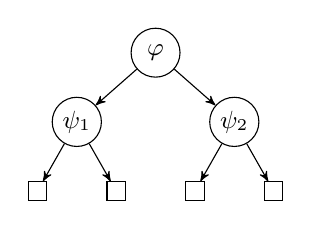
\begin{tikzpicture}[->,>=stealth',
	    level/.style={sibling distance=2cm/#1, level distance=25pt}]
	    \node [main node] (1){$\vph$}
	      child {node [main node,inner sep=1.7pt] (2) {$\psi_1$}
	      	child {node [rectangle,draw] (3) {}}
	      	child {node [rectangle,draw] (4) {}}
				}
	      child {node [main node,inner sep=1.7pt] (5) {$\psi_2$}
	      	child {node [rectangle,draw] (6) {}
					}
	      	child {node [rectangle,draw] (7) {}
					}
	      };
	  \end{tikzpicture}
  \caption{A preference tree}
%\vspace{-0.2cm}
  \label{fig:pt}
\end{figure}

%%%%We refer to trees such as the one in Figure \ref{fig:pt} as 
%%%%\emph{preference trees}, or \emph{P-trees}, for short. 
Trees such as the one in Figure \ref{fig:pt} are called \emph{preference 
trees}, or \emph{P-trees}. They were introduced by Fraser 
\cite{fraser1993,fraser1994}, who saw them as a convenient way to
represent conditional preferences. Despite their intuitive nature they
have not attracted much interest in the preference research in AI. In
particular, they were not studied for their relationship to other 
preference formalisms. The attribute of compact representations received 
only an informal treatment by Fraser (P-trees in their full representation
are often impractically large), and the algorithmic attributes of reasoning
with P-trees were also only touched upon. 


We propose an alternative definition of preference trees, 
and formally define their compact representation that exploits occurrences 
of identical subtrees. P-trees are reminiscent of LP-trees 
\cite{booth:learningLP}. We discuss the relation between the two concepts 
and show that P-trees offer a much more general, flexible and expressive 
way of representing preferences. We also discuss the relationship between 
preference trees and ASO preferences and possibilistic logic theories. 
We study the complexity of problems of comparing outcomes with respect 
to orders defined by preference trees, and of problems of finding optimal 
outcomes. 

This chapter is organized as follows. In the next section, we formally 
define P-trees and a compact way to represent them. In the following 
section we present results comparing the language of P-trees with other 
preference formalisms. We then move on to study the complexity of key 
reasoning tasks for preferences captured by P-trees and, finally, 
conclude by outlining some future research directions.


\section{Preference Trees}

In this section, we define preference trees and discuss their
representation. Let $\cI$ be a set of binary attributes\footnote{
	In case of multi-value attributes, $\cI$ is then a set of
	binary variables representing attribute values.
}. 
A \emph{preference tree} (\textit{P-tree}, for short) over $\cI$ is
a binary tree with all nodes other than 
leaves labeled with propositional formulas over $\cI$. Each P-tree 
$T$ defines a natural strict order $\succeq_T$ on the set of its leaves, 
the order of their enumeration from left to right. 

Given an outcome $o \in \CD(\cI)$, we define the \emph{leaf of $o$ in $T$}
as the leaf reached by starting at the root of $T$ and proceeding 
downwards. When at a node $t$ labeled with $\varphi$, if $o\models \varphi$, 
we descend to the left child of $t$; otherwise, we descend to the right node 
of $t$. We denote the leaf of $o$ in $T$ by $l_T(o)$.

We use the concept of the leaf of an outcome $o$ in a P-tree $T$ to 
define a total preorder on $\CD(\cI)$. Namely, for outcomes
$o_1, o_2\in \CD(\cI)$, 
we set $o_1\succeq_T o_2$, $o_1$ is \emph{preferred} to $o_2$, if $l_T(o_1) \succeq_T l_T(o_2)$, and
$o_1\succ_T o_2$, $o_1$ is \emph{strictly preferred} to $o_2$, 
if $l_T(o_1) \succ_T l_T(o_2)$.
(We overload the relations $\succeq_T$ and $\succ_T$ 
by using it both for the order on the leaves of $T$ 
and the corresponding preorder on the outcomes from $\CD(\cI)$). 
We say that $o_1$ is 
\emph{equivalent} to $o_2$, $o_1 \approx_T o_2$, if $l_T(o_1)=l_T(o_2)$. 
Finally, $o$ is \emph{optimal} if there exists no 
$o'$ such that $o' \succ_T o$.

Let us come back to the vacation example and assume that an agent 
prefers vacations involving water sports in Florida or hiking in Colorado
over the other options. This preference is described by the formula
$(x_1\land x_2) \lor (\neg x_1 \land \neg x_2)$ or, more concisely, as 
an equivalence $x_1 \equiv x_2$.
Within each of the two groups of vacations 
(satisfying the formula and not satisfying the formula), 
driving ($x_4$) is the preferred transporting mode. These preferences can be captured by the P-tree in
\figref{pt_vac_full}. We note that in this example, the preferences at 
the second level are \emph{unconditional}, that is, they do not depend on 
preferences at the top level. 

\begin{figure}[!ht]
        \centering
  \begin{subfigure}[b]{0.43\textwidth}
          \centering
          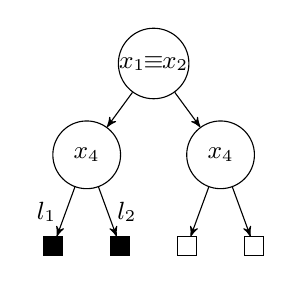
\begin{tikzpicture}[->,>=stealth',
            level/.style={sibling distance=1.7cm/#1, level distance=33pt}]
            \node [main node,inner sep=0pt] (1){$x_1 \!\! \equiv \!\! x_2$}
              child {node [main node,inner sep=5pt] (2) {$x_4$}
                child {node [rectangle,draw,fill] (3) {} edge from parent node[left] {\small{$l_1$}}}
                child {node [rectangle,draw,fill] (4) {} edge from parent node[right] {\small{$l_2$}}}
                                }
              child {node [main node,inner sep=5pt] (5) {$x_4$}
                child {node [rectangle,draw] (6) {}
                                        }
                child {node [rectangle,draw] (7) {}
                                        }
              };
          \end{tikzpicture}
          \caption{Full \label{fig:pt_vac_full}}
        \end{subfigure}%
  \begin{subfigure}[b]{0.43\textwidth}
          \centering
          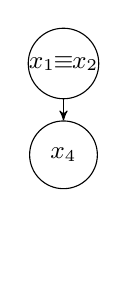
\begin{tikzpicture}[->,>=stealth',
            level/.style={sibling distance=2cm/#1, level distance=33pt}]
            \node [main node,inner sep=0pt] (1){$x_1 \!\! \equiv \!\! x_2$}
              child {node [main node,inner sep=5pt] (2) {$x_4$}
                        child {node [rectangle] (4) {} edge from parent[draw=none]}
                                };
          \end{tikzpicture}
          \caption{Compact \label{fig:pt_vac_compact}}
        \end{subfigure}
  \caption{P-trees on vacations}
%\vspace{-0.2cm}
  \label{fig:pt_vac}
\end{figure}

To compare two outcomes, $o_1=\neg x_1\neg x_2\neg x_3x_4$ 
and $o_2=x_1x_2x_3\neg x_4$,
we walk down the tree and find that $l_T(o_1)=l_1$ and $l_T(o_2)=l_2$. 
Thus, we have $o_1 \succ_T o_2$ since $l_1$ precedes $l_2$.


\ignore{
For a more complicated example, let us assume that an 
agent prefers vacations that take place in summer or involve hiking 
($\vph_1=\neg x_1 \lor x_3$) to all others, and this is the most 
desirable property to her. Among those vacations that satisfy $\vph_1$, 
the agent prefers hiking vacations in Colorado ($\vph_2 =\neg x_1 \land 
\neg x_2$) over the remaining ones in that group. Provided $\vph_1$ is 
satisfied, this is her second most important consideration. Her next 
concern for vacations satisfying 
$\vph_1$ is the mode of transportation. She prefers driving to flying 
for summer vacations and flying to driving, otherwise ($\vph_3= (x_3 
\rightarrow x_4) \land (\neg x_3 \rightarrow \neg x_4)$). Among vacations
that do not have the property $\vph_1$, that is, the vacations that are
in winter and involve water sports, the planner prefers to drive to 
Florida for her vacation ($\vph_2'=x_2 \land x_4$). The resulting
preference preorder on vacations can be represented as a P-tree $T$ 
shown in \figref{PTree_full}. This preorder has six clusters of
equivalent outcomes (vacation choices) represented by the six leaves,
with the decreasing preference for clusters of outcomes associated 
the leaves as we move from left to right. To compare two outcomes, $M
=\neg x_1x_2\neg x_3\neg x_4$ and $M'=x_1\neg x_2x_3\neg x_4$,
we walk down the trees and find that $l_T(M)=l_3$ and $l_T(M')=l_4$. 
Thus, $M \succ_T M'$ since $l_3$ precedes $l_4$.

\begin{figure}[!ht]
	\centering
  \begin{subfigure}[b]{0.23\textwidth}
		\centering
	  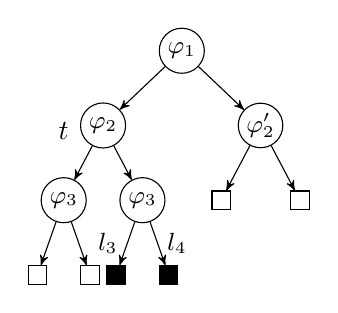
\begin{tikzpicture}[->,>=stealth',
	    level/.style={sibling distance=2cm/#1, level distance=27pt}]
	    \node [main node,inner sep=1.7pt] (1){$\varphi_1$}
	      child {node [main node,inner sep=1.7pt,label={[xshift=-0.5cm, yshift=-0.6cm]$t$}] (2) {$\varphi_2$}
	        child {node [main node,inner sep=1.7pt] (3) {$\varphi_3$}
	      		child {node [rectangle,draw] (4) {}}
	      		child {node [rectangle,draw] (5) {}}
					}
	        child {node [main node,inner sep=1.7pt] (6) {$\varphi_3$}
	      		child {node [rectangle,draw,fill] (7) {} edge from parent node[left] {\small{$l_3$}}}
	      		child {node [rectangle,draw,fill] (8) {} edge from parent node[right] {\small{$l_4$}}}
					}
				}
	      child {node [main node,inner sep=0.9pt] (9) {$\varphi_2'$}
	      	child {node [rectangle,draw] (10) {}
					}
	      	child {node [rectangle,draw] (11) {}
					}
	      };
	  \end{tikzpicture}
		\caption{Full representation \label{fig:PTree_full}}
	\end{subfigure}%
  \begin{subfigure}[b]{0.23\textwidth}
		\centering
	  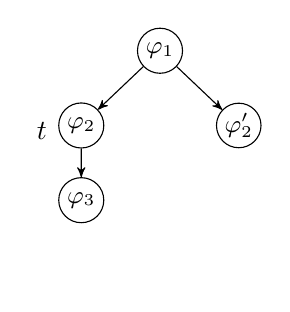
\begin{tikzpicture}[->,>=stealth',
	    level/.style={sibling distance=2cm/#1, level distance=27pt}]
	    \node [main node,inner sep=1.7pt] (1){$\varphi_1$}
	      child {node [main node,inner sep=1.7pt,label={[xshift=-0.5cm, yshift=-0.6cm]$t$}] (2) {$\varphi_2$}
	        child {node [main node,inner sep=1.7pt] (3) {$\varphi_3$}
	      		child {node [rectangle] (4) {} edge from parent[draw=none]}
					}
				}
	      child {node [main node,inner sep=0.9pt] (5) {$\varphi_2'$}
	      	child {node [rectangle] (6) {} edge from parent[draw=none]}
	      };
	  \end{tikzpicture}
		\caption{Compact representation \label{fig:PTree_compact}}
	\end{subfigure}
  \caption{P-trees}
%\vspace{-0.2cm}
  \label{fig:PTree}
\end{figure}
}

The key property of P-trees is that they can represent any total preorder on 
$\CD(\cI)$.

\begin{prop}
\label{prop:1}
For every set $\cI$ of binary attributes, for every set $D\subseteq\CD(\cI)$
of outcomes over $\cI$, and for every total preorder $\succeq$ on $D$ into
no more than $2^n$ clusters of equivalent outcomes, there is a P-tree $T$ 
of depth at most $n$ such that the preorder determined by $T$ on $\CD(\cI)$ 
when restricted to $D$ coincides with $\succeq$ 
(that is, ${\succeq_T}_{|D}=\succeq$).
\end{prop}
\begin{proof}
Let $\succeq$ be a total preorder on a subset $D\subseteq \CD(\cI)$ of outcomes
over $\cI$, and let $D_1\succ D_2\succ \ldots\succ D_m$ be the corresponding 
strict ordering of clusters of equivalent outcomes, with $m\leq 2^n$. If
$m=1$, a single-leaf tree (no decision nodes, just a box node) represents 
this preorder. This tree has depth 0 and so, the assertion holds. Let us assume
then that $m>1$, and let us define $D'=D_1\cup\ldots\cup D_{\lceil m/2\rceil}$ 
and $D''=D\setminus
D'$. Let $\varphi_{D'}$ be a formula such that models of $D'$ 
are precisely the outcomes in $D'$ (such a formula can be constructed as a
disjunction of conjunctions of literals, each conjunction representing a
single outcome in $D'$). If we place $\varphi_{D'}$ in the root of a P-tree,
that tree represents the preorder with two clusters, $D'$ and $D''$, with 
$D'$ preceding $D''$. Since each of $D'$ and $D''$ has no more than $2^{n-1}$
clusters, by induction, the preorders $D_1\succ \ldots\succ 
D_{\lceil m/2\rceil}$ and $D_{\lceil m/2\rceil+1}\succ \ldots\succ D_m$ 
can each be represented as a P-tree with depth at most $n-1$. Placing
these trees as the left and the right subtrees of $\varphi_{D'}$ 
respectively results in a P-tree of depth at most $n$ that represents
$\succeq$. 
\end{proof}

\paragraph{\bf Compact Representation of P-Trees.}
Proposition \ref{prop:1} shows high expressivity 
of P-trees. However, the construction described in the proof has little 
practical use. First, the P-tree it produces may have a 
large size due to the large sizes of labeling formulas that are generated. 
Second, to apply it, one would need to have an explicit enumeration of 
the preorder to be modeled, and that explicit representation in practical 
settings is unavailable.         

However, preferences over combinatorial domains that arise in practice
typically have structure that can be elicited from a user and exploited
when constructing a P-tree representation of the preferences. First,
decisions at each level are often based on considerations involving
only very few attributes, often just one or two and very rarely more than that.
Moreover, the subtrees of a node that order the ``left'' and the``right''
outcomes are often identical or similar. 

Exploiting these features often leads to much smaller representations.  
A \emph{compact P-tree over} $\cI$ is a tree such that
\begin{enumerate}[itemsep=0pt]
	\item every node is labeled with a Boolean formula over $\cI$, and
  \item every non-leaf node $t$ labeled with $\varphi$ has either
        two outgoing edges, with the left one meant to be taken by 
        outcomes that satisfy $\varphi$ and the right one by those that
        make $\varphi$ false (\figref{compact1}), or one 
    outgoing edge pointing
    \begin{itemize}[itemsep=0pt]
      \item straight-down (\figref{compact2}), which indicates that the two subtrees of $t$ 
            are \textit{identical} and the formulas
            labeling every pair of corresponding nodes in the two subtrees are the \textit{same},
      \item left (\figref{compact3}), which indicates that right subtree 
      of $t$ is empty, or
      \item right (\figref{compact4}), which indicates that left subtree 
      of $t$ is empty.
    \end{itemize}
\end{enumerate}

\begin{figure}[!ht]
	\centering
  \begin{subfigure}[b]{0.3\textwidth}
		\centering
	  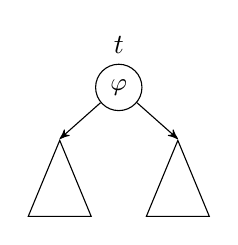
\begin{tikzpicture}[->,>=stealth',
	    level/.style={sibling distance=1.5cm/#1, level distance=30pt}]
	    \node [main node,inner sep=3pt,label={[xshift=0cm, yshift=0cm]$t$}] (1){$\varphi$}
				child [edge from parent path ={(\tikzparentnode.-140) -- (\tikzchildnode.north)}] {
					node [subtree,yshift=0.4cm] (2) {}}
				child [edge from parent path ={(\tikzparentnode.-40) -- (\tikzchildnode.north)}] {
					node [subtree,yshift=0.4cm] (3) {}};
	  \end{tikzpicture}
		\caption{\label{fig:compact1}}
	\end{subfigure}%
  \begin{subfigure}[b]{0.2\textwidth}
		\centering
	  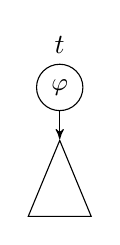
\begin{tikzpicture}[->,>=stealth',
	    level/.style={sibling distance=1.5cm/#1, level distance=30pt}]
		    \node [main node,inner sep=3pt,label={[xshift=0cm, yshift=0cm]$t$}] (1){$\varphi$}
					child {node [subtree,yshift=0.4cm] (2) {}};
	  \end{tikzpicture}
		\caption{\label{fig:compact2}}
	\end{subfigure}%
  \begin{subfigure}[b]{0.2\textwidth}
		\centering
		  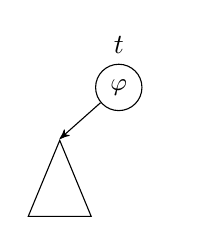
\begin{tikzpicture}[->,>=stealth',
		    level/.style={sibling distance=1.5cm/#1, level distance=30pt}]
		    \node [main node,inner sep=3pt,label={[xshift=0cm, yshift=0cm]$t$}] (1){$\varphi$}
					child [edge from parent path ={(\tikzparentnode.-140) -- (\tikzchildnode.north)}] {
						node [subtree,yshift=0.4cm] (2) {}}
	      		child {node [rectangle] (3) {} edge from parent[draw=none]
		      };
		  \end{tikzpicture}
			\caption{\label{fig:compact3}}
	\end{subfigure}%
  \begin{subfigure}[b]{0.2\textwidth}
		\centering
	  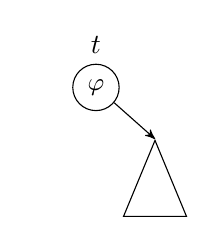
\begin{tikzpicture}[->,>=stealth',
	    level/.style={sibling distance=1.5cm/#1, level distance=30pt}]
		    \node [main node,inner sep=3pt,label={[xshift=0cm, yshift=0cm]$t$}] (1){$\varphi$}
	      	child {node [rectangle] (2) {} edge from parent[draw=none]
		      }
					child [edge from parent path ={(\tikzparentnode.-40) -- (\tikzchildnode.north)}] {
						node [subtree,yshift=0.4cm] (2) {}};
	  \end{tikzpicture}
		\caption{\label{fig:compact4}}
	\end{subfigure}
  \caption{Compact P-trees}
%\vspace{-0.2cm}
  \label{fig:compact}
\end{figure}


The P-tree in \figref{pt_vac_full} can be collapsed as both 
subtrees of the root are the same (including the labeling formulas). This 
leads to a tree in \figref{pt_vac_compact} with a straight-down edge.
\ignore{
Let $t$ be a node in a P-tree $T$.  
We denote by $\Inst(t)$ the set of 
ancestor nodes of $t$ in $T$ that have two outgoing edges.
}
\ignore{
Similarly, in the P-tree 
in \figref{PTree_full}, the two subtrees of node $t$ and the formulas 
labeling the corresponding nodes are identical. Thus, we can collapse 
them and achieve a compact representation in \figref{PTree_compact}. 
}
We note that we drop box-labeled leaves in compact representations 
of P-trees, as they no longer have an interpretation as distinct clusters.

\paragraph{\bf Empty Leaves in P-Trees.} Given a P-tree $T$ one can prune it
so that all sets of outcomes corresponding to its leaves are non-empty.
However, keeping empty clusters may lead to compact representations of much
smaller (in general, even exponentially smaller) size.

%A compact P-tree $T$ in \figref{PTree_EL_compact} represents a full 
%binary tree $T'$ in \figref{PTree_EL_full}.
%The formulas labeling the non-leaf nodes in $T$ are $\varphi_1=\neg x_1 \vee x_3$, $\varphi_2=x_2 \vee \neg x_4$
%and $\varphi_3=x_2 \wedge x_3$.
%We can check that leaves $l_1$, $l_2$ and $l_3$ are empty, that is,
%the conjunctions $\varphi_1 \wedge \neg \varphi_2 \wedge \varphi_3$,
%$\neg \varphi_1 \wedge \varphi_2 \wedge \varphi_3$ and
%$\neg \varphi_1 \wedge \neg \varphi_2 \wedge \varphi_3$ are
%unsatisfiable.
A full P-tree $T$ in \figref{PTree_EL_full} uses labels
$\varphi_1=\neg x_1 \vee x_3$, $\varphi_2=x_2 \vee \neg x_4$, and
$\varphi_3=x_2 \wedge x_3$.
We check that leaves $l_1$, $l_2$ and $l_3$ are empty, that is,
the conjunctions $\varphi_1 \wedge \neg \varphi_2 \wedge \varphi_3$,
$\neg \varphi_1 \wedge \varphi_2 \wedge \varphi_3$ and
$\neg \varphi_1 \wedge \neg \varphi_2 \wedge \varphi_3$ are
unsatisfiable.
Pruning $T$ one obtains a compact tree $T'$ (\figref{PTree_NEL_compact}) that is
smaller compared to $T$, but larger than $T''$ (\figref{PTree_EL_compact}), another compact 
representation of $T$, should we allow empty leaves and exploit
the structure of $T$.

\begin{figure}[!ht]
	\centering
  \begin{subfigure}[b]{0.4\textwidth}
		\centering
	  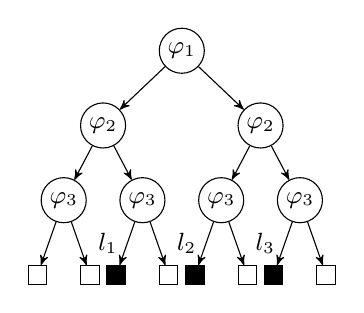
\begin{tikzpicture}[->,>=stealth',
	    level/.style={sibling distance=2cm/#1, level distance=27pt}]
	    \node [main node,inner sep=1.7pt] (1){$\varphi_1$}
	      child {node [main node,inner sep=1.7pt] (2) {$\varphi_2$}
	        child {node [main node,inner sep=1.7pt] (3) {$\varphi_3$}
	      		child {node [rectangle,draw] (4) {}}
	      		child {node [rectangle,draw] (5) {}}
					}
	        child {node [main node,inner sep=1.7pt] (6) {$\varphi_3$}
	      		child {node [rectangle,draw,fill] (7) {} edge from parent node[left] {\small{$l_1$}}}
	      		child {node [rectangle,draw] (8) {}}
					}
				}
	      child {node [main node,inner sep=1.7pt] (9) {$\varphi_2$}
	        child {node [main node,inner sep=1.7pt] (10) {$\varphi_3$}
	      		child {node [rectangle,draw,fill] (11) {} edge from parent node[left] {\small{$l_2$}}}
	      		child {node [rectangle,draw] (12) {}}
					}
	        child {node [main node,inner sep=1.7pt] (13) {$\varphi_3$}
	      		child {node [rectangle,draw,fill] (14) {} edge from parent node[left] {\small{$l_3$}}}
	      		child {node [rectangle,draw] (15) {}}
					}
	      };
	  \end{tikzpicture}
		\caption{$T$ \label{fig:PTree_EL_full}}
	\end{subfigure}%
  \begin{subfigure}[b]{0.4\textwidth}
		\centering
		  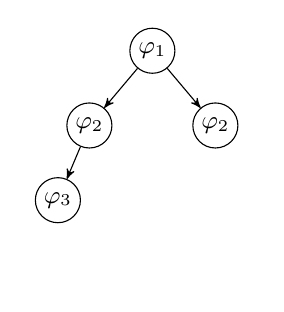
\begin{tikzpicture}[->,>=stealth',
		    level/.style={sibling distance=1.6cm/#1, level distance=27pt}]
		    \node [main node,inner sep=1.7pt] (1){$\varphi_1$}
		      child {node [main node,inner sep=1.7pt] (2) {$\varphi_2$}
		        child {node [main node,inner sep=1.7pt] (3) {$\varphi_3$}
		      		child {node [rectangle] (4) {} edge from parent[draw=none]}
		      		child {node [rectangle] (5) {} edge from parent[draw=none]}
						}
		        child {node [rectangle] (6) {} edge from parent[draw=none]
						}
					}
		      child {node [main node,inner sep=1.7pt] (7) {$\varphi_2$}
		        child {node [rectangle] (8) {} edge from parent[draw=none]}
		        child {node [rectangle] (9) {} edge from parent[draw=none]}
		      };
		  \end{tikzpicture}
			\caption{$T'$: pruned $T$\label{fig:PTree_NEL_compact}}
	\end{subfigure}%
  \begin{subfigure}[b]{0.2\textwidth}
		\centering
	  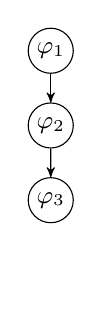
\begin{tikzpicture}[->,>=stealth',
	    level/.style={sibling distance=2cm/#1, level distance=27pt}]
	    \node [main node,inner sep=1.7pt] (1){$\varphi_1$}
	      child {node [main node,inner sep=1.7pt] (2) {$\varphi_2$}
	        child {node [main node,inner sep=1.7pt] (3) {$\varphi_3$}
	      		child {node [rectangle] (4) {} edge from parent[draw=none]}
					}
				};
	  \end{tikzpicture}
		\caption{$T''$ \label{fig:PTree_EL_compact}}

	\end{subfigure}
  \caption{P-trees with empty leaves}
%\vspace{-0.2cm}
  \label{fig:PTree_EL}
\end{figure}

That example generalizes and leads to the question
of finding small sized representations of P-trees.
(We conjecture that the
problem in its decision version asking about the existence of a compact 
representation of size at most $k$ is NP-complete). 
From now on, we assume that P-trees are given in their compact representation. 

%\begin{figure}[!ht]
%	\centering
%	  \begin{tikzpicture}[->,>=stealth',
%	    level/.style={sibling distance=2cm/#1, level distance=27pt}]
%	    \node [main node,inner sep=1.7pt] (1){$\varphi_1$}
%	      child {node [main node,inner sep=1.7pt] (2) {$\varphi_2$}
%	        child {node [main node,inner sep=1.7pt] (3) {$\varphi_3$}
%	      		child {node [rectangle,draw] (4) {}}
%	      		child {node [rectangle,draw] (5) {}}
%					}
%	        child {node [rectangle,draw] (6) {}
%					}
%				}
%	      child {node [main node,inner sep=1.7pt] (7) {$\varphi_2$}
%	        child {node [rectangle,draw] (8) {}}
%	        child {node [rectangle,draw] (9) {}}
%	      };
%	  \end{tikzpicture}
%		\caption{$T''$: pruned $T'$}
%\vspace{-0.2cm}
%  \label{fig:PTree_full_NEL}
%\end{figure}

\section{P-Trees and Other Formalisms}

In this section we compare the preference representation language of P-trees
with other preference languages.


\paragraph{\bf P-Trees Generalize LP-Trees.}

As stated earlier, P-trees are reminiscent of LP-trees, a preference 
language that has received significant attention recently 
\cite{booth:learningLP,lang:aggLP,LiuT}. In fact, LP-trees over a set
$\cI=\{x_1,\ldots,x_n\}$ of attributes are simply special P-trees over $\cI$.
Namely, an LP-tree over $\cI$ can be defined as a P-tree over $\cI$, in
which all formulas labeling nodes are atoms $x_i$ or their negations $\neg x_i$,
depending on whether $x_i$ or $\neg x_i$ is the preferred over the other, and every path from 
the root to a leaf has all atoms $x_i$ appear in it as labels exactly 
once. Clearly, LP-trees are full binary trees of depth $n$ (assuming the depth of the root is 1) 
and determine strict \emph{total orders} on outcomes 
in $\CD(\cI)$ (no indifference between different outcomes). An example 
of an LP-tree over $\{x_1,x_2,x_3,x_4\}$ for our vacation example is 
given in \figref{LPT_full}. 

\begin{figure}[!ht]
	\centering
	  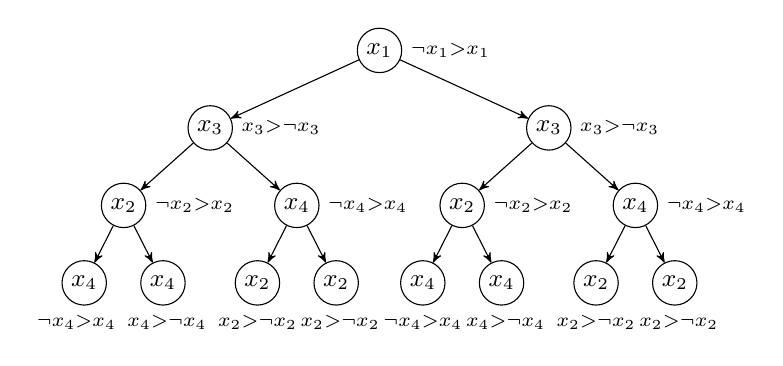
\begin{tikzpicture}[->,>=stealth',
       level 1/.style={sibling distance=4.3cm, level distance=28pt},
       level 2/.style={sibling distance=2.2cm, level distance=28pt},
       level 3/.style={sibling distance=1.0cm, level distance=28pt}]
	    \node [main node,inner sep=2pt,label={[xshift=0.9cm, yshift=-0.5cm]$\scriptstyle \neg x_1>x_1$}] (1){$x_1$}
	    child {node [main node,inner sep=2pt,label={[xshift=0.9cm, yshift=-0.5cm]$\scriptstyle x_3>\neg x_3$}] (2) {$x_3$}
	      child {node [main node,inner sep=2pt,label={[xshift=0.9cm, yshift=-0.5cm]$\scriptstyle \neg x_2>x_2$}] (3) {$x_2$}
	        child {node [main node,inner sep=2pt,label={[xshift=-0.1cm, yshift=-1cm]$\scriptstyle \neg x_4>x_4$}] (4) {$x_4$}}
	        child {node [main node,inner sep=2pt,label={[xshift=0.05cm, yshift=-1cm]$\scriptstyle x_4>\neg x_4$}] (5) {$x_4$}}
				}
	      child {node [main node,inner sep=2pt,label={[xshift=0.9cm, yshift=-0.5cm]$\scriptstyle \neg x_4>x_4$}] (6) {$x_4$}
	        child {node [main node,inner sep=2pt,label={[xshift=0cm, yshift=-1cm]$\scriptstyle x_2>\neg x_2$}] (7) {$x_2$}}
	        child {node [main node,inner sep=2pt,label={[xshift=0.05cm, yshift=-1cm]$\scriptstyle x_2>\neg x_2$}] (8) {$x_2$}}
	      }
			}
	    child {node [main node,inner sep=2pt,label={[xshift=0.9cm, yshift=-0.5cm]$\scriptstyle x_3>\neg x_3$}] (9) {$x_3$}
	      child {node [main node,inner sep=2pt,label={[xshift=0.9cm, yshift=-0.5cm]$\scriptstyle \neg x_2>x_2$}] (10) {$x_2$}
	        child {node [main node,inner sep=2pt,label={[xshift=0cm, yshift=-1cm]$\scriptstyle \neg x_4>x_4$}] (11) {$x_4$}}
	        child {node [main node,inner sep=2pt,label={[xshift=0.05cm, yshift=-1cm]$\scriptstyle x_4> \neg x_4$}] (12) {$x_4$}}
				}
	      child {node [main node,inner sep=2pt,label={[xshift=0.9cm, yshift=-0.5cm]$\scriptstyle \neg x_4>x_4$}] (13) {$x_4$}
	        child {node [main node,inner sep=2pt,label={[xshift=0cm, yshift=-1cm]$\scriptstyle x_2>\neg x_2$}] (14) {$x_2$}}
	        child {node [main node,inner sep=2pt,label={[xshift=0.05cm, yshift=-1cm]$\scriptstyle x_2>\neg x_2$}] (15) {$x_2$}}
	      }
			}
			;
	  \end{tikzpicture}
  \caption{A full LP-tree on vacations}
%	\vspace{-0.2cm}
  \label{fig:LPT_full}
\end{figure}

In general representing preferences by LP-trees is impractical. The size of
the representation is of the same order as that of an explicit enumeration
of the preference order. However, in many cases preferences on outcomes 
have structure that leads to LP-trees with similar subtrees. That structure
can
be exploited, as in P-trees, to represent LP-trees compactly.  
\figref{LPT_PT_lpt} shows a compact representation of the LP-tree in  
\figref{LPT_full}. We note the presence of conditional preference tables 
that make up for the lost full binary tree structure. Together with the 
simplicity of the language, compact representations are behind the practical 
usefulness of LP-trees. The compact representations of LP-trees translate 
into compact representations of P-trees, in the sense defined above. This 
matter is not central to our discussion and we simply illustrate it with 
an example. The compactly represented P-tree in \figref{LPT_PT_pt} is the
counterpart to the compact LP-tree in \figref{LPT_PT_lpt},
where $\varphi=(x_2 \land x_4) \lor (\neg x_2 \land \neg x_4)$.

\begin{figure}[!ht]
	\centering
  \begin{subfigure}[b]{0.43\textwidth}
		\centering
	  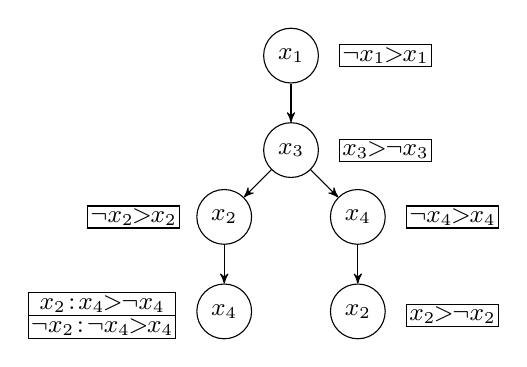
\begin{tikzpicture}[->,>=stealth',node distance=1.2cm]
	        
	    \node[main node] (1) {$x_1$};
	    \node[rectangle,draw,inner sep=1pt] at (1.2,0) {$\neg x_1\!\! >\!\! x_1$};
	
	    \node[main node] (2) [below of=1] {$x_3$};
	    \node[rectangle,draw,inner sep=1pt] at (1.2,-1.2) {$x_3 \!\!>\!\! \neg x_3$};
	    
	    \node[main node] (3) [below left of=2] {$x_2$};
	    \node[rectangle,draw,inner sep=1pt] at (-2,-2.05) {$\neg x_2 \!\!>\!\! x_2$};
	    
	    \node[main node] (4) [below of=3] {$x_4$};
	    \node[rectangle split, rectangle split parts=2, draw,inner sep=1pt,font=\sffamily\small] at (-2.4,-3.3)
	        {
	          $x_2\!:\!x_4 \!\!>\!\! \neg x_4$
	          \nodepart{second}
	          $\neg x_2\!:\!\neg x_4 \!\!>\!\! x_4$
	        };
	    
	    \node[main node] (5) [below right of=2] {$x_4$};
	    \node[rectangle,draw,inner sep=1pt] at (2.05,-2.05) {$\neg x_4\!\! > \!\! x_4$};
	    
	    \node[main node] (6) [below of=5] {$x_2$};
	    \node[rectangle,draw,inner sep=1pt] at (2.05,-3.3) {$x_2 \!\!>\!\! \neg x_2$};
	  
	    \path[every node/.style={font=\sffamily\small}]
	      (1) edge (2)
	      (2) edge (3)
	          edge (5)
	      (3) edge (4)
	      (5) edge (6);
	  \end{tikzpicture}
  	\caption{A compact LP-tree \label{fig:LPT_PT_lpt}}
	\end{subfigure}%
	\begin{subfigure}[b]{0.43\textwidth}
			\centering
		  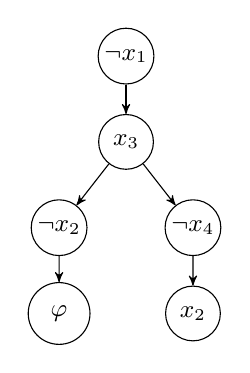
\begin{tikzpicture}[->,>=stealth',
		    level/.style={sibling distance=3.4cm/#1, level distance=31pt}]
		    \node [main node,inner sep=1.5pt] (1){$\neg x_1$}
		    child {node [main node] (2) {$x_3$}
		      child {node [main node,inner sep=1.5pt] (3) {$\neg x_2$}
		        child {node [main node,inner sep=5pt] (4) {$\varphi$}
		      		%child {node [rectangle] (5) {} edge from parent[draw=none]}
						}
					}
		      child {node [main node,inner sep=1.5pt] (6) {$\neg x_4$}
		        child {node [main node] (7) {$x_2$}
		      		%child {node [rectangle] (8) {} edge from parent[draw=none]}
						}
		      }};
		  \end{tikzpicture}
  		\caption{The corresponding P-tree \label{fig:LPT_PT_pt}}
		\end{subfigure}
  \caption{A compact LP-tree as a compact P-tree}
%\vspace{-0.2cm}
  \label{fig:LPT_PT}
\end{figure}

The major drawback of LP-trees is that they can capture only a very small
fraction of preference orders. One can show that the number, say $G(n)$, 
of LP-trees over $n$ attributes is 
\begin{equation*}
G(n)=\prod_{k=0}^{n-1} (n-k)^{2^k} \cdot 2^{2^k}
\end{equation*}
and is asymptotically much smaller than $L(n)=(2^n)!$, the number of all 
preference orders of the corresponding domain of outcomes. In fact, 
one can show that 
\[
\frac{G(n)}{L(n)} < \frac{1}{2^{(2^n \cdot (n-\log n -2))}}.
\]
This is in stark contrast with Proposition \ref{prop:1}, according
to which every total preorder can be represented by a P-tree.

Even very natural orderings, which have simple (and compact) representations
by P-trees often cannot be represented as LP-trees. For instance, there is 
no LP-tree on $\{x_1,x_2\}$ representing the order $00\succ 11 \succ 01 
\succ 10\}$. However, the P-trees (both full and compact) in \figref{pt_vac}
do specify it.

\ignore{
We show in \thmref{exp_small_ratio} that
LP-trees only encode an exponentially small portion of all linear orders.
\begin{thm}
\label{thm:exp_small_ratio}
	Let $L(n)=2^n!$ be the number of linear orders of outcomes over $n$ binary attributes,
	$r$ be the ratio of $G(n)$ to $L(n)$.
	We have
	\begin{equation}
		r = \frac{G(n)}{L(n)} < \frac{1}{2^{(2^n \cdot (n-\log n -2))}}.
	\end{equation}
\end{thm}
%\begin{proof}
%	\begin{align*}
%		r 2^n! &= T(n); \numberthis \\
%		\log r + \log 2^n! &= \log (\prod_{k=0}^{n-1} (n-k)^{2^k} \cdot 2^{2^k})\\
%		&= \sum_{k=0}^{n-1} (\log ((n-k)^{2^k}) + 2^k)\\
%		&= \sum_{k=0}^{n-1} (2^k \cdot (\log (n-k) + 1))\\
%		&< \sum_{k=0}^{n-1} (2^k \cdot (\log n + 1))\\
%		&= (\log n + 1) \cdot \sum_{k=0}^{n-1} 2^k\\
%		&= (\log n + 1) \cdot (2^n-1). \numberthis 
%	\end{align*}
%	
%	Let $N$ be such that $N=(\log n + 1) \cdot (2^n-1)$.
%	By the Stirling's approximation $n! \geq \sqrt{2\pi n} \cdot (\frac{n}{e})^n$,
%	we have the following.
%	
%	\begin{align*}
%		\log r &< N - \log 2^n! \\
%		&\leq N- \log (\sqrt{2\pi 2^n} \cdot (\frac{2^n}{e})^{2^n})\\
%		&< N- \log (\sqrt{2^n} \cdot (\frac{2^n}{e})^{2^n})\\
%		&= N- (\frac{n}{2}+\log \frac{2^{n\cdot 2^n}}{e^{2^n}})\\
%		&= N- (\frac{n}{2}+n\cdot 2^n-\log e^{2^n})\\
%		&< N- (\frac{n}{2}+n\cdot 2^n-\log 2^{2^n})\\
%		&= N- (\frac{n}{2}+n\cdot 2^n-2^n)\\
%		&= 2^n \cdot (\log n -n+2)-\log n-1-\frac{n}{2}\\
%		&< 2^n \cdot (\log n -n+2). \numberthis
%	\end{align*}
%	
%	Therefore, we have
%	\begin{equation}
%		r < \frac{1}{2^{(2^n \cdot (n-\log n -2))}}.
%	\end{equation}
%\end{proof}
}

\paragraph{\bf P-Trees Extend ASO-Rules.} The formalism of ASO-rules 
\cite{Brewka:ASO} provides an intuitive way to express preferences
over outcomes as total preorders.
An ASO-rule partitions outcomes into ordered clusters according to 
the semantics of the formalism.
Formally, an ASO-rule $r$ over $\cI$ is a preference rule of the form
\begin{equation} \label{eq:ASO}
\small{C_1 > \ldots > C_m \leftarrow B,}
\end{equation}

\noindent
where all $C_i$'s and $B$ are propositional formulas over $\cI$.
For each outcome $M$, rule (\ref{eq:ASO}) determines its \emph{satisfaction degree}.
It is denoted by $\SD_r(M)$ and defined by
\[
\small{\SD_r(M) =
  \begin{cases}
   1, & M \models \neg B \\
   m+1, & M \models B \wedge \bigwedge_{1 \leq i \leq m} \neg C_i \\
   min\{i:M \models C_i\}, & \mbox{otherwise}.
  \end{cases}}
\]

\noindent
We say that an outcome $M$ is weakly preferred to an 
outcome $M'$ ($M
\succeq_r M'$) if $\SD_r(M)\leq\SD_r(M')$. Thus, the notion of the 
satisfaction degree (or, equivalently, the preference $r$) partitions
outcomes into (in general) $m+1$ clusters.\footnote{This definition is 
a slight adaptation of the original one.}

Let us consider the domain of vacations.
An agent may prefer hiking in Colorado to water sports in Florida if she
is going on a summer vacation.
Such preference can be described as an ASO-rule:
\begin{center}
	$\neg x_1 \land \neg x_2 > x_1 \land x_2 \leftarrow x_3$.
\end{center}
Under the semantics of ASO, this preference rule specifies that
the most desirable vacations are summer hiking vacations to Colorado
and all winter vacations, the next preferred vacations are
summer water sports vacations to Florida, and the least desirable vacations
are summer hiking vacations to Florida and summer water sports vacations to Colorado.

Given an ASO-rule $r$ of form (\ref{eq:ASO}),
we show how $r$ is encoded in a P-tree.
From the ASO-rule $r$, we build a P-tree $T_r$ in \figref{ASO_P},
where $\varphi_1 = \neg B \vee C_1$,
$\varphi_i =C_i$ ($2 \leq i \leq m$),
and the dashed edge represents nodes labeled by the formulas $\varphi_3,\ldots,\varphi_{m-1}$
and every formula $\varphi_i$, $3 \leq i \leq m-1$, is constructed such that
the parent of $\varphi_i$ is $\varphi_{i-1}$, the left child of $\varphi_i$
is empty, and the right child of $\varphi_i$ is $\varphi_{i+1}$.

\begin{figure}
  \small
  \centering
	  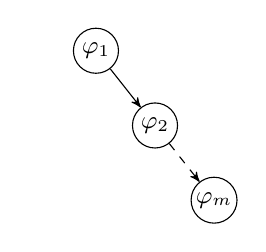
\begin{tikzpicture}[->,>=stealth',
        level 1/.style={sibling distance=1.5cm, level distance=27pt},
        level 2/.style={sibling distance=1.5cm, level distance=27pt}
        ]
	    \node [main node,inner sep=1.7pt] (1){$\varphi_1$}
	      child {node [rectangle] (2) {} edge from parent[draw=none]}
	      child {node [main node,inner sep=1.7pt] (3) {$\varphi_2$}
	      	child {node [rectangle] (4) {} edge from parent[draw=none]}
					child {node [main node,inner sep=0.9pt] (5) {$\varphi_m$} [dashed]
						%child [solid] {node [rectangle,draw] (6) {}}
					}
				};
	  \end{tikzpicture}
  \caption{A P-tree $T_r$ ($T_P$)}
%\vspace{-0.2cm}
  \label{fig:ASO_P}
\end{figure}

\begin{thm}
\label{thm:ASO_P}
	Given an ASO-rule $r$, the P-tree $T_r$ has size
	linear in the size of $r$, and for every two outcomes $M$ and $M'$
	\begin{center}
		$M \succeq_r^{\textit{ASO}} M' \;\; \textit{iff} \;\; M \succeq_{T_r} M'$
	\end{center}
\end{thm}
\begin{proof}
	The P-tree $T_r$ induces a total preorder $\succeq_{T_r}$ where outcomes satisfying $\varphi_1$ are preferred
	to outcomes satisfying $\neg \varphi_1 \land \varphi_2$, which are then preferred to
	outcomes satisfying $\neg \varphi_1 \land \neg \varphi_2 \land \varphi_3$, and so on.
	The least preferred are the ones satisfying $\bigwedge_{1\leq i\leq m} \neg \varphi_i$.
	Clearly, this order $\succeq_{T_r}$ is precisely the order $\succeq^{\textit{ASO}}_r$
	given by the ASO rule $r$.
\end{proof}

%Clearly, the size of $T_r$ is linear in the size of the input $r$.
There are other ways of translating ASO-rules to P-trees. For instance,
it might be beneficial if the translation produced a more balanced tree.
Keeping the definitions of $\vph_i$, $1\leq i\leq m$, as 
before and setting $\vph_{m+1}=B \land \neg C_1 \land \ldots \land \neg 
C_m$, we could proceed as in the proof of \propref{1}. %for $m+1$ clusters. 
%First, create the root node $N$ of $T^b_r$ and label it with the formula
%$\bigvee_{1 \leq i \leq \lfloor \frac{m+2}{2} \rfloor} \varphi_i$.
%Then, proceed recursively to construct $N$'s left subtree $T_1$ for 
%$\varphi_1,\ldots,\varphi_{\lfloor \frac{m+2}{2} \rfloor}$,
%and $N$'s right subtree $T_2$ for $\varphi_{\lfloor \frac{m+2}{2} \rfloor+1},
%\ldots, \varphi_{m+1}$.

For example, if $m=6$, we build the P-tree $T^b_r$ in \figref{PTree_tp},
where $\psi_1=\varphi_1 \vee \varphi_2 \vee \varphi_3 \vee \varphi_4$,
$\psi_2=\varphi_1 \vee \varphi_2$, $\psi_3=\varphi_1$, $\psi_4=\varphi_3$,
$\psi_5=\varphi_5 \vee \varphi_6$, and $\psi_6=\varphi_5$.
The indices $i$'s of the formulas $\psi_i$'s indicate the order in which
the corresponding formulas are built recursively.


\begin{figure}[!ht]
	\centering
	  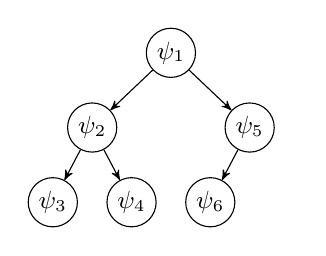
\begin{tikzpicture}[->,>=stealth',
	    level/.style={sibling distance=2cm/#1, level distance=27pt}]
	    \node [main node,inner sep=1.7pt] (1){$\psi_1$}
	      child {node [main node,inner sep=1.7pt] (2) {$\psi_2$}
	        child {node [main node,inner sep=1.7pt] (3) {$\psi_3$}
	      		%child {node [rectangle,draw] (4) {}}
	      		%child {node [rectangle,draw] (5) {}}
					}
	        child {node [main node,inner sep=1.7pt] (6) {$\psi_4$}
	      		%child {node [rectangle,draw] (7) {}}
	      		%child {node [rectangle,draw] (8) {}}
					}
				}
	      child {node [main node,inner sep=1.7pt] (9) {$\psi_5$}
	        child {node [main node,inner sep=1.7pt] (10) {$\psi_6$}
	      		%child {node [rectangle,draw] (11) {}}
	      		%child {node [rectangle,draw] (12) {}}
					}
	        child {node [rectangle] (13) {} edge from parent[draw=none]}
	      };
	  \end{tikzpicture}
		\caption{$T^b_r$ when $m=6$}
%\vspace{-0.2cm}
  \label{fig:PTree_tp}
\end{figure}

This P-tree representation of a preference $r$ of the form (\ref{eq:ASO}) 
is balanced with height $\lceil \log_2 (m+1) \rceil$. Moreover, 
the property in \thmref{ASO_P} also holds for the balanced $T^b_r$
of size polynomial in the size of $r$.
In fact, the size of $T^b_r$ is in $O(s_r \log s_r)$, where $s_r$ is
the size of rule $r$.
It is clear that, though tree $T^b_r$ is larger than $T_r$ in size,
comparing outcomes could be done faster due to a smaller depth of $T^b_r$.

\paragraph{\bf Representing P-Trees as RASO-Theories.}

Preferences represented by compact P-trees cannot in general be
captured by ASO preferences without a significant (in some cases,
exponential) growth in the size of the representation. However, any 
P-tree can be represented as a set of \emph{ranked} ASO-rules, 
or an RASO-theory \cite{Brewka:ASO}, aggregated by the Pareto method.

\nop{Introduce RASO and Pareto method}
We first show how Pareto method is used to order outcomes with regard
to a set of \emph{unranked} ASO-rules. Let $M$ and $M'$ be two outcomes.  
Given a set $P$ of unranked ASO-rules, $M$ is weakly preferred to $M'$ 
with respect to $P$, $M \succeq^u_P M'$, if $\SD_r(M) \leq \SD_r(M')$ 
for every $r \in P$. Moreover, $M$ is strictly preferred to $M'$, $M 
\succ^u_P M'$, if $M \succeq^u_P M'$ and $\SD_r(M) < \SD_r(M')$ for some 
$r \in P$, and $M$ is equivalent to $M'$, $M \approx^u_P M'$,
if $\SD_r(M) = \SD_r(M')$ for every $r \in P$.

In general, the resulting preference relation is not total. However, by 
ranking rules according to their importance in some cases, total preorders
can be obtained. Let us assume $P=\{P_1,\ldots,P_g\}$ is a collection of 
ranked ASO preferences divided into $g$ sets $P_i$, with each set $P_i$ 
consisting 
of ASO-rules of rank $d_i$ so that $d_1 < d_2<\ldots d_g$. We assume that 
a lower rank of a preference
rule indicates its higher importance.
We define $M 
\succeq^{rk}_P M'$ w.r.t $P$ if for every $i$, $1\leq i\leq g$, 
$M \approx^u_{P_i} M'$, or if there exists a rank $i$ such that 
$M \approx^u_{P_j} M'$ for every $j$, $j< i$, and $M \succ^u_{P_i} M'$.

Given a P-tree $T$, we construct an RASO-theory $\Phi_T$ as follows.
We start with $\Phi_T=\emptyset$.
For every node $t_i$ in a P-tree $T$, we update
$\Phi_T=\Phi_T \cup \{\varphi_i \overset{d_i}{\leftarrow} conditions\}$,
where $\varphi_i$ is the formula labeling node $t_i$,
$d_i$, rank of the ASO-rule, is the depth of node $t_i$,
and $conditions$ is the conjunction
of formulas $\varphi_j$ or $\neg \varphi_j$ labeling all nodes $t_j$
%such that $t_j \in \Inst(t_i)$.
that are ancestor nodes of $t_i$ in $T$ with two outgoing edges.
Whether $\varphi_j$ or $\neg \varphi_j$ is used depends on how the path 
from the root to
$t_i$ determines whether descending left ($\varphi_j$) or right ($\neg \varphi_j$)
at $t_j$.

For instance, the P-tree $T$ in \figref{LPT_PT_pt} gives rise to the following RASO-theory:

	\begin{framed}
%\vspace{-0.2cm}
		\noindent $\neg x_1 \overset{1}{\leftarrow}$.  \\%$\;\;\;\;\;$
		$x_3 \overset{2}{\leftarrow}$.\\
		$\neg x_2 \overset{3}{\leftarrow} x_3$.  $\;\;\;\;\;$
		$\neg x_4 \overset{3}{\leftarrow} \neg x_3$.\\
		$(x_2 \land x_4) \lor (\neg x_2 \land \neg x_4) \overset{4}{\leftarrow} x_3$. $\;\;\;\;\;$
		$x_2 \overset{4}{\leftarrow} \neg x_3$.
%\vspace{-0.2cm}
	\end{framed}

\begin{thm}
\label{thm:P_RASO}
	Given a P-tree $T$, there exists an RASO-theory $\Phi_T$ of size
	polynomial in the size of $T$ such that for every two outcomes $M$ and $M'$
	\begin{center}
		$M \succeq_{\Phi_T}^{\textit{RASO}} M' \;\; \textit{iff} \;\; M \succeq_{T} M'$
	\end{center}
\end{thm}
%\noindent Proof of \thmref{P_RASO} is omitted due to space constraint.
\begin{proof}
($\Leftarrow$) Let us assume $M \succeq_{T} M'$.
Denote by $(\varphi_{i_1},\ldots,\varphi_{i_j})$ the order of formulas 
labeling the path determined by $M$ from the root to a leaf.
Let $\varphi_{i_k}$, $1 \leq k \leq j$, be the first formula that
$M$ and $M'$ evaluate differently, in fact, $M \models \varphi_{i_k}$
and $M' \not \models \varphi_{i_k}$.
Denote by $d$ the depth of $\varphi_{i_k}$ in $T$.
Based on the construction of $\Phi_T$, 
for every RASO-rule $r$ of rank less than $d$, we have
$M \approx_{r}^{\textit{ASO}} M'$. For every RASO-rule $r$
of rank $d$, we have $M \succ_{r}^{\textit{ASO}} M'$ if
$r$ comes from $\varphi_{i_k}$; $M \approx_{r}^{\textit{ASO}} M'$
for other rules of rank $d$.
According to RASO ordering, $M \approx_{\Phi_T}^{\textit{RASO}} M'$ holds
if $\varphi_{i_k}$ does not exist; $M \succ_{\Phi_T}^{\textit{RASO}} M'$
holds, otherwise.  Therefore, $M \succeq_{\Phi_T}^{\textit{RASO}} M'$ holds.

($\Rightarrow$) Prove by contradiction.  We assume that $M \succeq_{\Phi_T}^{\textit{RASO}} M'$ 
and $M' \succ_{T} M$ hold.
We again denote by $(\varphi_{i_1},\ldots,\varphi_{i_j})$ the order of formulas
labeling the path determined by $M$ from the root to a leaf.
There must exist some formula $\varphi_{i_k}$, $1 \leq k \leq j$, such that
$M' \models \varphi_{i_k}$, $M \not \models \varphi_{i_k}$, and
all formulas $\varphi_\ell$, $1 \leq \ell \leq k-1$, are evaluated in the same way
by $M$ and $M'$. Based on RASO ordering, we have $M' \succ_{\Phi_T}^{\textit{RASO}} M$,
contradiction.
\end{proof}

Hence, the relationship between P-trees and ASO preferences can be summarized as follows.
Every ASO preference rule can be translated into a P-tree, and 
every P-tree into a theory of ranked ASO preference rules.
In both cases, the translations have size polynomial in the size of the input.
Examining the reverse direction, the size of the ASO rule translated from a P-tree
could be exponential, and the orders represented by ranked ASO theories
\emph{strictly include} the orders induced by P-trees as RASO-theories describe
\emph{partial} preorders in general.

\paragraph{\bf P-Trees Extend Possibilistic Logic.}

\nop{\comm{DEFINE THE SEMANTICS OF POSS LOG}}

A possibilistic logic theory $\Pi$ over a vocabulary $\cI$ is a set of 
\emph{preference pairs}
\begin{center}
	$\{ (\phi_1,a_1), \ldots, (\phi_m,a_m) \}$,
\end{center}
where every $\phi_i$ is a Boolean formula over $\cI$, and every $a_i$ is a real number
such that $1\geq a_1>\ldots>a_m\geq 0$ (if two formulas have the same 
importance level, they can be replaced by their conjunction).
Intuitively, $a_i$ represents the importance of $\phi_i$, with larger values
indicating higher importance.

The \textit{tolerance degree} of outcome $M$ with regard to preference 
pair $(\phi,a)$, $\TD_{(\phi,a)}(M)$, is defined by
\[
 \TD_{(\phi,a)}(M) =
  \begin{cases}
   1, & M \models \phi \\
   1-a, & M \not \models \phi
  \end{cases}
\]
Based on that, the tolerance degree of outcome $M$ with regard to a \emph{set}
$\Pi$ of preference pairs, $\TD_\Pi(M)$, is defined by 
\begin{center}
	$\TD_\Pi(M)=min\{\TD_{(\phi_i,a_i)}(M):1\leq i \leq m\}$.
\end{center}
The larger $\TD_\Pi(M)$, the more preferred $M$ is.

For example, for the domain of vacations, we might have the following
set of preference pairs $\{(\neg x_1 \wedge x_3,0.8), (x_2 \wedge x_4,0.5)\}$.
According to the possibilistic logic interpretation, vacations satisfying 
both preferences are the most preferred, those satisfying $\neg x_1 \wedge x_3$ 
but falsifying $x_2 \wedge x_4$ are the next
preferred, and those falsifying $\neg x_1 \wedge x_3$ are the worst.

Similarly as for ASO-rules, we can apply different methods to encode 
a possibilistic logic theories in P-trees. Here we discuss one of them.
We define $T_\Pi$ to be an unbalanced P-tree shown in \figref{ASO_P} with with 
labels $\varphi_i$ defined as follows: 
$\varphi_1=\bigwedge_{\substack{1\leq i \leq m}} \phi_i$, 
$\varphi_2=\bigwedge_{\substack{1\leq i \leq m-1}} \phi_i \wedge \neg \phi_m$,
$\varphi_3=\bigwedge_{\substack{1\leq i \leq m-2}} \phi_i \wedge \neg \phi_{m-1}$, and
$\varphi_m = \phi_1 \wedge \neg \phi_2$.
%$\varphi_{m+1}=\neg \phi_1$.

%\begin{figure}
%  \small
%  \centering
%	  \begin{tikzpicture}[->,>=stealth',
%	    level/.style={sibling distance=1.5cm/#1}]
%	    \node [main node] (1){$\varphi_1$}
%	      child {node [rectangle,draw] (2) {}
%				}
%	        child {node [main node] (3) {$\varphi_m$} [dashed]
%						child [solid] {node [rectangle,draw] (4) {}}
%					};
%	  \end{tikzpicture}
%  \caption{A P-tree $T_P$}
%  \label{fig:Poss_P}
%\end{figure}

\begin{thm}
\label{thm:Poss_P}
	Given a possibilistic theory $\Pi$, there exists a P-tree $T_\Pi$ of size
	polynomial in the size of $\Pi$ such that for every two outcomes $M$ and $M'$
	\begin{center}
		$M \succeq_\Pi^{\textit{Poss}} M' \;\; \textit{iff} \;\; M \succeq_{T_\Pi} M'$
	\end{center}
\end{thm}
\begin{proof}
	%Note that both induce in general total preorders of $m+1$ clusters.
	%It is clear that
	%outcome $M$ is in the $i$-th cluster induced by $\Pi$ if and only if
	%it is in the $i$-th cluster induced by $T_\Pi$.
	It is clear that the size of P-tree $T_\Pi$ is polynomial in the size of $\Pi$.
	Let $mi(M,\Pi)$ denote the maximal index $j$ such that $M$ satisfies
	all $\phi_1, \ldots, \phi_j$ in $\Pi$.
	(If $M$ falsifies all formulas in $\Pi$, we have $mi(M,\Pi)=0$.)
	One can show that $M \succeq_\Pi^{\textit{Poss}} M'$ if and only if
	$mi(M,\Pi) \geq mi(M',\Pi)$, and $mi(M,\Pi) \geq mi(M',\Pi)$ if and only
	if $M \succeq_{T_\Pi} M'$.  Therefore, the theorem follows.
\end{proof}



\section{Reasoning Problems and Complexity}

In this section, we study decision problems on reasoning about preferences described as
P-trees, and provide computational complexity results for the three reasoning
problems defined below.

\begin{definition}
\label{def:dom}
  Dominance-testing ({\sc DomTest}): given a P-tree $T$ and two distinct outcomes
  $M$ and $M'$, decide whether $M \succeq_T M'$.
\end{definition}

\begin{definition}
\label{def:opt_test}
  Optimality-testing ({\sc OptTest}): given a P-tree $T$ and an outcome $M$ of $T$,
  decide whether $M$ is optimal.
\end{definition}

\begin{definition}
\label{def:opt_prop}
  Optimality-with-property ({\sc OptProp}): given a P-tree $T$ and some property $\alpha$ 
	expressed as a Boolean formula 
	over the vocabulary of $T$,
  decide whether there is an optimal outcome $M$ that satisfies $\alpha$.
\end{definition}

Our first result shows that P-trees support efficient dominance testing.
\begin{thm}
\label{thm:dom}
	The {\sc DomTest} problem can be solved in time linear in the
	height of the P-tree $T$.
\end{thm}
\begin{proof}
	The {\sc DomTest} problem can be solved by walking down the tree.
	The preference between $M$ and $M'$ is determined at the first non-leaf node
	$n$ where $M$ and $M'$ evaluate $\varphi_n$ differently.  If such
	node does not exist before arriving at a leaf, $M \approx_T M'$.
\end{proof}
An interesting reasoning problem not mentioned above is to decide whether 
there exists an optimal outcome with respect to the order given by a P-tree.
However, this problem is trivial as the answer simply depends on whether 
there is any outcome at all. However, optimality \emph{testing} is a 
different matter. Namely, we have the following result.

\begin{thm}
\label{thm:opt_test}
	The {\sc OptTest} problem is coNP-complete.
\end{thm}
\begin{proof}
%	Need to show that deciding whether the given outcome $M$ is \textit{not} an optimal 
%	outcome in a given P-tree $T$ is NP-complete.
%	This complement problem is  in class NP because one can guess an outcome $M'$ in
%	polynomial time and verify in polynomial time that $M' \succ_T M$.
%	Hardness follows from a polynomial time reduction from SAT \cite{Garey:1979}.
%	Details of the reduction is omitted due to limited space.
%	(Membership) The problem is in class NP because one can guess an outcome $M'$ in
%	polynomial time and verify in polynomial time that $M' \succ M$.
%
%	(Hardness) The hardness follows from a polynomial time reduction from SAT \cite{Garey:1979}.
We show that the complementary problem, testing non-optimality of an outcome
$M$, is NP-complete. Membership is obvious. A witness of non-optimality of $M$
is any outcome $M'$ such that $M' \succ_T M$, a property that can be verified 
in linear time (cf. Theorem \ref{thm:dom}).
	NP-hardness follows from a polynomial time reduction from SAT \cite{Garey:1979}.
	Given a CNF formula $\Phi=c_1\land\ldots\land c_n$ over a set of variables
	$V=\{X_1,\ldots,X_m\}$, we construct a P-tree $T$ and an outcome $M$
as follows.
\begin{enumerate}
\item We choose $X_1,\ldots,X_m,unsat$ as attributes, where $unsat$ is 
a new variable;
\item we define the P-tree $T_\Phi$ (cf. \figref{P_opt_2_comp}) to consist of a 
single node labeled by $\Psi=\Phi \land \neg unsat$;
\item we set $M=\{unsat\}$.
\end{enumerate}

	We show that $M=\{unsat\}$ is not an optimal outcome if and only if
	$\Phi=\{c_1,\ldots,c_n\}$ is satisfiable.

\noindent
	($\Rightarrow$) Assume that $M=\{unsat\}$ is not an optimal outcome.
	Since $M \not \models \Psi$, $M$ belongs to the right
	leaf and there must exist an outcome $M'$ such that $M' \succ M$.
	This means that $M' \models \Phi \wedge \neg unsat$. Thus, 
	$\Phi$ is satisfiable.

\noindent
	($\Leftarrow$) Let $M'$ be a satisfying assignment to $\Phi$ over $\{X_1,\ldots,X_m\}$.
	Since no $c_i \in \Phi$ mentions $unsat$, we can assume $unsat \not \in M'$.
	So $M' \models \Psi$ and $M'$ is optimal.
	Thus, $M=\{unsat\}$ is not optimal.
\end{proof}

\begin{figure}
  \centering
	  
\begin{tikzpicture}[->,>=stealth',
	    level/.style={sibling distance=1.5cm/#1, level distance=30pt}]
	    \node [main node,inner sep=4pt] (1){$\Psi$}
	      %child {node [rectangle,draw] (2) {}}
				;
	  \end{tikzpicture}
  \caption{The P-tree $T_\Phi$}
%\vspace{-0.2cm}
  \label{fig:P_opt_2_comp}
\end{figure}


\begin{thm}
\label{thm:opt_prop}
	The {\sc OptProp} problem is $\deltap{2}$-complete.
\end{thm}
\begin{proof}
	(Membership) The problem is in the class $\deltap{2}$. Let $T$ be a given
	preference tree. To check whether there is an optimal outcome that 
	satisfies a property $\alpha$, we start at the root of $T$ and move down.
	As we do so, we maintain the information about the path we took by 
	updating a formula $\psi$, which initially is set to $\top$ (a generic
	tautology). Each time we move down to the left from a node $t$, we 
	update $\psi$ to $\psi\land\vph_t$, and when we move down to the right,
	to $\psi\land\neg\vph_t$. To decide whether to move down left or right 
	form a node $t$, we check if $\vph_{t} \land \psi$ is satisfiable by 
	making a call to an NP oracle for deciding satisfiability. If $\vph_{t} 
	\land \psi$ is satisfiable, we proceed to the left subtree and, 
	otherwise, to the right one. We then update $t$ to be the node we moved 
	to and repeat. When we reach a leaf of the tree (which represents a
	cluster of outcomes), this cluster is non-empty, consists of all 
	outcomes satisfying $\psi$ and all these outcomes are optimal. Thus, 
	returning YES, if $\psi\land \alpha$ is satisfiable and NO, otherwise, 
	correctly decides the problem. Since the number of oracle calls is 
	polynomial in the size of the tree $T$, the problem is in the class
	$\deltap{2}$. 

\medskip
\noindent
	(Hardness) The maximum satisfying assignment (MSA) problem\footnote{
		Given a Boolean formula $\Phi$ over $\{x_1,\ldots,x_n\}$, the
		maximum satisfying assignment (MSA) problem is to decide whether $x_n=1$ 
		in the lexicographically maximum satisfying assignment for $\Phi$.
		(If $\Phi$ is unsatisfiable, the answer is $\no$.)
	}
	\cite{Krentel:88} is $\deltap{2}$-complete.
	We first show that MSA remains $\deltap{2}$-hard if we
	restrict the input to Boolean formulas that are satisfiable and 
        have models other than
	the all-false model (i.e., $\neg x_1\ldots\neg x_n$).

	\begin{lem}
	\label{lem:MSA_sat}
		The MSA problem is $\deltap{2}$-complete when $\Phi$ is satisfiable and has models
		other than the all-false model.
	\end{lem}
	\begin{proof}
		Given a Boolean formula $\Phi$ over $\{x_1,\ldots,x_n\}$, we define
		$\Psi=\Phi \lor (x_0\land\neg x_1 \land\ldots \land\neg x_n)$ over
		$\{x_0,x_1,\ldots,x_n\}$.
		It is clear that $\Psi$ is satisfiable, and has at least one model other than
		the all-false one.
		Let $M$ be a lexicographically maximum assignment satisfying $\Phi$ and
		$M$ has $x_n=1$.
		Extending $M$ by $x_0=1$ yields a lexicographically maximum assignment 
		satisfying $\Psi$ and this assignment satisfies $x_n=1$.
		Conversely, if $M$ is a lexicographically maximum assignment satisfying $\Psi$
		and $x_n=1$ holds in $M$, it follows that $M \models \Phi$.  Thus,
		restricted $M$ to $\{x_1,\ldots,x_n\}$, the assignment is lexicographically maximal
		satisfying $\Phi$.
	\end{proof}

	We now show the hardness of the {\sc OptProp} problem by a reduction from this
	restricted version of the MSA problem. Let $\Phi$
	be a satisfiable propositional formula over variables $x_1,\ldots,x_n$ 
	that has at least one model other than the all-false one.
	We construct an instance of the {\sc OptProp} problem as follows.
	We define the P-tree $T_\Phi$ as shown in \figref{P_opt_3_comp}, 
where every node is labeled by formula $\Phi \land x_i$, and we set
	$\alpha=x_n$.

	\begin{figure}
	  \small
	  \centering
		  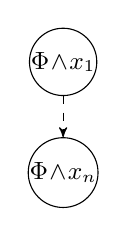
\begin{tikzpicture}[->,>=stealth',
		    level/.style={sibling distance=2.5cm/#1, level distance=40pt}]
		    \node [main node,inner sep=0pt] (1){$\Phi \! \land \! x_1$}
		      child {node [main node,inner sep=0pt] (2) {$\Phi \! \land \! x_n$} [dashed]
		      	%child [solid] {node [rectangle,draw] (3) {}}
		      };
		  \end{tikzpicture}
	  \caption{The P-tree $T_\Phi$}
%\vspace{-0.2cm}
	  \label{fig:P_opt_3_comp}
	\end{figure}

	Our P-tree $T_\Phi$ induces a total preorder consisting of a sequence of
	singleton clusters, each containing an outcome satisfying $\Phi$,
	followed by a single cluster comprising all outcomes that falsify
	$\Phi$ and the all-false model.
	By our assumption on $\Phi$, the total preorder has at least 
        two non-empty clusters.
	Moreover, all singleton clusters
	preceding the last one are ordered lexicographically. Thus, the optimal 
	outcome of $T_\Phi$ satisfies $\alpha$ if and only if the lexicographical
	maximum satisfying outcome of $\Phi$ satisfies $x_n$.
\end{proof}

%\section{Aggregating P-Trees}
%In the setting of multi-agent systems when agents that collaborate
%with each other need to make a common decision, it is important to
%aggregate their individual preferences in order to reach a collective agreement.
%We adopt two approaches to solve aggregation problems of P-trees:
%the Pareto method and voting rules.
%
%\subsection{The Pareto method}
%%When an agent express her preferences in terms of a set of P-trees, it is important to consider these P-trees
%%together to compute optimal outcomes to support further decision making process.
%%For instance, in a recommendation system preferences are aggregated so that the top $K$ outcomes are computed.
%We define the Pareto method problem and present its implementation using answer set programming (ASP) 
%\cite{mt99:stable}.
%
%
%\begin{definition}
%\label{def:opt_pareto}
%  Optimality-testing-Pareto ({\sc OptTestPa}): given a set $P$ of P-trees
%	and an outcome $M$,
%	decide whether $M$ is a Pareto optimal outcome with regard to $P$.
%\end{definition}
%
%\begin{definition}
%\label{def:dom_pareto}
%  Dominance-testing-Pareto ({\sc DomTestPa}): given a set $P$ of P-trees
%	and an outcome $M$,
%	decide whether there exists another outcome $M'$ such that $M' \succ_P M$,
%	that is, $M$ is Pareto dominated by $M'$ with respect to $P$.
%\end{definition}
%
%The {\sc OptTestPa} problem is \textit{coNP-complete}, 
%and the {\sc DomTestPa} problem is \textit{NP-complete}.
%It is clear that the {\sc OptTestPa} problem is in coNP.
%Hardness of {\sc OptTestPa} follows from \thmref{opt_test} where a single P-tree is considered.
%As for the {\sc DomTestPa} problem, obviously it is in NP, and its hardness is due to
%the fact that its solution leads to the solution of the complement of {\sc OptTestPa}.
%
%The implementation is based on a testing program in ASP that takes an outcome as input and computes
%a strictly better one if such an outcome exists.
%The computation starts with an arbitrary outcome which is given to the testing program.
%If the testing program fails to generate a strictly better outcome, the input outcome is Pareto
%optimal with regard to $P$.  If the testing program generates such an outcome that is strictly
%better, the new outcome becomes the input and the process repeats until Pareto optimality is reached.
%
%\smallskip \noindent \textbf{Encoding P-trees as logic programming rules.}
%A P-tree can be encoded as a set of logic programming rules.
%To solve the {\sc OptTestPa} problem, we need to encode P-trees in such a way that
%the dominance between two outcomes can be determined.
%
%Let $\varphi_i$ be the formula that labels a node $t$ in a P-tree $T$ at depth $d^T_i$,
%$\Inst(t)=\{t_1,\ldots, t_j\}$ where each $t_q$, $1\leq q \leq j$, 
%is labeled by a formula $\varphi_{i_q}$.
%The location of $t$ is determined by its
%depth $d^T_i$ and by how the formulas $\varphi_{i_1},\ldots,\varphi_{i_j}$
%labeling $\Inst(t)$ are evaluated (they determine whether we descend to the left or
%to the right child as we descend down the tree).
%Thus, the preferences with $\varphi_i$ can be represented by the following
%logic programming rule.
%\begin{equation} \label{eq:prefASP}
%\begin{split}
%  \small
%  pt&(T,d^T_i,i) \; \ifLparse \; \form(T,i_1), \ldots, \form(T,i_k), \\
%    &not \; \form(T,i_{k+1}), \ldots, not \; \form(T,i_j), \form(T,i).
%\end{split}
%  \end{equation}
%In rule (\eqtref{prefASP}), predicate $\form(T,\ell)$ holds for an outcome $M$ 
%if in P-tree $T$ outcome $M$ satisfies
%formula $\varphi_\ell$, and predicate $pt(T,d^T_i,i)$ holds for $M$ if
%in $T$ outcome $M$ satisfies formula $\varphi_i$ at depth $d^T_i$.
%The rule indicates that $pt(T,d^T_i,i)$ holds for $M$
%if in $T$ outcome $M$ satisfies formulas $\varphi_{i_1},\ldots,\varphi_{i_k} \in \Inst(t)$,
%falsifies formulas $\varphi_{i_{k+1}},\ldots,\varphi_{i_j} \in \Inst(t)$,
%and satisfies formula  $\varphi_i$.
%
%Let us recall the example P-tree $T$ in \figref{PTree_compact} and represent the P-tree as
%a set of logic rules in \figref{P_ASP}, where predicate $outcome(X_i,a)$ holds
%for outcome $M$ if $M$ assigns value $a$ to variable $X_i$.
%
%\begin{figure}[ht!]
%	\begin{framed}
%\footnotesize
%		\begin{verbatim}
%1  id(1).
%2  form(1,1) :- outcome(1,1).
%3  form(1,2) :- outcome(2,1), outcome(3,1).
%4  form(1,3) :- outcome(4,0).
%5  form(1,4) :- outcome(2,0), outcome(4,1).
%6  pt(1,1,1) :- form(1,1).
%7  pt(1,2,2) :- form(1,1), form(1,2).
%8  pt(1,2,4) :- not form(1,1), form(1,4).
%9  pt(1,3,3) :- form(1,1), form(1,3).
%		\end{verbatim}
%	\end{framed}
%	\caption{Encode $T$ in ASP}
%  \label{fig:P_ASP}
%\end{figure}
%
%
%\smallskip \noindent \textbf{The $P$-dominance-Pareto problem in ASP.}
%We assume the starting outcome $M$ is $\vec{0}$, that is, an outcome assigning
%0 to all variables. The testing program $P$ is built by adding the following rules
%to the encoding of $P$:
%\begin{enumerate}
%	\item For each formula $\varphi_i \in P$ such that $M \models \varphi_i$, include a fact 
%				$pt\_start(T,d^T_i,i)$ where $T$ is the id of the P-tree that 
%				$\varphi_i$ comes from, and $d^T_i$ is the depth of $\varphi_i$ in $T$.
%	\item Include the rules in \figref{P_dom_encod}.
%\end{enumerate}
%
%\begin{figure}[ht!]
%	\begin{framed}
%\footnotesize
%		\begin{verbatim}
% 1  1{ outcome(X,Y) : val(Y) }1 :- var(X).
% 
% 2  split_depth(ID,D) :- pt(ID,D,F), 
%      not pt_start(ID,D,F).
% 3  split_depth(ID,D) :- not pt(ID,D,F), 
%      pt_start(ID,D,F).
% 4  first_split_depth(ID,D) :- id(ID), 
%      D=#min[split_depth(ID,Depth)=Depth].
% 
% 5  eq(ID) :- id(ID), 
%      first_split_depth(ID,#supremum).
% 6  better(ID) :- first_split_depth(ID,D), 
%      D != #supremum, pt(ID,D,F).
% 7  bettereq(ID) :- eq(ID).
% 8  bettereq(ID) :- better(ID).
% 
% 9  :- not exist_better.
%10  exist_better :- better(ID).
%11  :- id(ID), not bettereq(ID).
%		\end{verbatim}
%	\end{framed}
%	\caption{Encode the {\sc DomTestPa} problem in ASP}
%  \label{fig:P_dom_encod}
%\end{figure}
%
%
%
%\subsection{Voting rules}
%As P-trees are in general total preorders over outcomes,
%we consider voting rules to aggregate them, such as positional scoring rules
%(Plurality, $k$-Approval, Borda, etc), Maximin, and Copeland.
%
%\tc{
%	Votes with empty leaves make a difference when we apply positional scoring
%	rules on them, whereas they do not matter for comparison-based voting rules.
%	So for positional scoring rules, do we consider votes with empty leaves valid or invalid?
%	If invalid, we need to identify those votes and discard them from the profile, but
%	checking if one P-tree is invalid takes exponentially many calls of the SAT oracle
%	in the worst case!
%	If valid, we still need to compute, for every P-tree, which leaves are
%	empty, which again takes exponentially many calls to a SAT solver!
%	However, I think that one can assume all votes are carefully specified
%	so that empty leaf does not exist.
%}
%
%\smallskip \noindent \textbf{Plurality.}
%Assume for vote (P-tree) $T$ there are $c$ outcomes with rank 1.
%If $c=0$, it means that $T$ vetos all outcomes, thus $T$ is an invalid
%vote and is removed from the profile.
%Otherwise, every top-ranked outcome gets score $\frac{1}{c}$.
%Understanding the Plurality this way, we need to know the number of top-ranked
%outcomes in every P-tree.  The problem of ``counting the number of
%outcomes that satisfy a formula $\Phi$" is \#P-hard.
%
%\smallskip \noindent \textbf{Copeland.}
%As proved by Lang et al \cite{lang:aggLP}, for LP-trees in classes $\{UI,CI\} \times \{UP,CP\}$,
%computing the Copeland score of a given outcome in a given profile is \#P-complete,
%and the Maximin evaluation problem is coNP-complete.
%These results should still hold in the setting of P-trees which extend the
%framework of LP-trees.


\section{Conclusions}

We investigated the qualitative preference representation language of 
\textit{preference trees}, or \textit{P-trees}. This language was 
introduced in early 1990s (cf. \cite{fraser1993,fraser1994}), but have 
not received a substantial attention as a formalism for preference 
representation in AI. We studied formally the attribute of compact 
representations of
P-trees, established its relationship to other preference languages
such as lexicographic preference trees, possibilistic logic and
answer-set optimization. For several preference reasoning problems 
on P-trees we derived their their computational complexity.

P-trees are quite closely related to possibilistic logic theories or
preference expressions in answer-set optimization. However, they allow
for much more structure among formulas appearing in these latter two
formalisms (arbitrary trees as opposed to the linear structure of 
preference formulas in the other two formalisms). This structure allows 
for representations of conditional preferences. P-trees are also more
expressive than lexicographic preference trees. This is the case even 
for P-trees in which every node is labeled with a formula involving just
two attributes, as we illustrated with the $00\succ 11\succ 01\succ 01$ 
example. Such P-trees are still simple enough to correspond well to
the way humans formulate hierarchical models of preferences, with all
their decision conditions typically restricted to one or two attributes. 

Our paper shows that P-trees form a rich preference formalism that
deserves further studies. Among the open problems of interest are 
those of learning P-trees and their compact representations, aggregating
P-trees coming from different sources (agents), and computing
optimal consensus outcomes. These problems will be considered in the 
future work. 

%Note the copyright notice at the end of each chapter.
\copyrightnotice

\chapter{Learning Partial Lexicographic Preference Trees\label{ch:learningPLPT}}
We introduce \tit{partial lexicographic preference trees} (PLP-trees) 
as a formalism for compact representations of preferences over 
combinatorial domains. Our main results concern the problem of passive 
learning of PLP-trees. Specifically, for several classes of 
PLP-trees, we study how to learn (i) a PLP-tree consistent with a 
dataset of examples, possibly subject to requirements on the size 
of the tree, and (ii) a PLP-tree correctly ordering as many of 
the examples as possible in case the dataset of examples is inconsistent. 
We establish complexity of these problems and, in all cases where the 
problem is in the class P, propose polynomial time algorithms.

\section{Introduction}
%Representing and reasoning about preferences are fundamental to decision
%making and so, of significant interest to artificial intelligence. When 
%the choice is among a few \emph{outcomes} (\emph{alternatives}),
%representations in terms of explicit enumerations of the preference order 
%are feasible and lend themselves well to formal analysis. However, in many
%applications outcomes come from \emph{combinatorial domains}. That is,
%outcomes are described as tuples of values of \emph{attributes} (also 
%referred to as \emph{variables} or \emph{attributes}), say $X_1,\ldots, 
%X_p$, with each attribute $X_i$ assuming values from some set $D_i$ -- its 
%\emph{domain}. 
%Because of the combinatorial size of the space of such outcomes, explicit
%enumerations of their elements are impractical. Instead, we resort to 
%formalisms supporting intuitive and, ideally, concise \emph{implicit}
%descriptions of the order. The language of CP-nets \cite{bbdh03} is a prime
%example of such a formalism. 

Recently, there has been a rising interest in representing
preferences over combinatorial domains by exploiting the notion of
the lexicographic ordering. For instance, assuming attributes are over the  
binary domain $\{0,1\}$, with the preferred value for each attribute being 
1, a sequence of attributes naturally determines an order on outcomes.
This idea gave rise to the language of \tit{lexicographic preference 
models} or \tit{lexicographic strategies}, which has been extensively 
studied in the literature \cite{schmitt2006complexity,dombi2007learning,%
yaman2008democratic}. The formalism of complete \tit{lexicographic 
preference trees} (LP-trees) \cite{booth:learningLP} generalizes the
language of lexicographic strategies by arranging attributes into 
decision trees that assign preference ranks to outcomes. An important
aspect of LP-trees is that they allow us to model \emph{conditional}
preferences on attributes and \emph{conditional} ordering of attributes. 
Another formalism,
the language of \tit{conditional lexicographic preference trees} (or 
CLP-trees) \cite{brauning2012learning}, extends LP-trees by allowing 
subsets of attributes as labels of nodes.

A central problem in preference representation concerns learning 
implicit models of preferences (such as lexicographic strategies,
LP-trees or CLP-trees), of possibly small sizes, that are consistent 
with all (or at least possibly many) given examples, each correctly 
ordering a pair of outcomes. The problem was extensively studied. Booth
et al. \shortcite{booth:learningLP} considered learning of LP-trees, and 
Br\"auning and Eyke \shortcite{brauning2012learning} of CLP-trees. 

In this work, we introduce \emph{partial lexicographic preference trees} (or 
\emph{PLP-trees}) as means to represent \emph{total preorders} over 
combinatorial domains. PLP-trees are closely related to LP-trees 
requiring that every path in the tree contains all attributes 
used to describe outcomes. Consequently, LP-trees describe total 
orders over the outcomes. PLP-trees relax this requirement and allow 
paths on which some attributes may be missing. Hence, 
PLP-trees describe total preorders. This seemingly small difference
has a significant impact on some of the learning problems. It allows
us to seek PLP-trees that minimize the set of attributes on their paths,
which may lead to more robust models by disregarding attributes 
that have no or little influence on the true preference (pre)order.

The rest of the chapter is organized as follows. In the next section, 
we introduce the language of PLP-trees and describe a classification 
of PLP-trees according to their complexity. We also define three types of passive 
learning problems for the setting of PLP-trees. In the following 
sections, we present algorithms learning PLP-trees of particular
types and computational complexity results on the existence of 
PLP-trees of different types, given size or accuracy. We close 
with conclusions and a brief account of future work.


\section{Partial Lexicographic Preference Trees}
Let $\cI=\{X_1,\ldots,X_p\}$ be a set of binary attributes, with each
$X_i$ having its domain $D_i=\{0_i, 1_i\}$. The corresponding 
\tit{combinatorial domain} is the set $\cX=D_1 \times \ldots \times D_p$.
Elements of  $\cX$ are called \tit{outcomes}.

A PLP-tree over $\cX$ is binary tree whose every
non-leaf node is labeled by an attribute from $\cI$ and by a preference
entry $1>0$ or $0>1$, and whose every leaf node is denoted by a box 
$\Box$. Moreover, we require that on every path from the root to a leaf
each attribute appears \emph{at most} once. 

To specify the total preorder on outcomes defined by a PLP-tree $T$, let 
us enumerate leaves of $T$ from left to right, assigning them 
integers $1,2$, etc. For every outcome $\alpha$ we find its leaf 
in $T$ by starting at the root of $T$ and proceeding downward. 
When at a node labeled with an attribute $X$, we descend to the left or to the 
right child of that node based on the value $\alpha(X)$ of the attribute $X$ 
in $\alpha$ and on the preference assigned to that node. If $\alpha(X)$ is 
the preferred value, we descend to the left child. We descend to the right
child,
otherwise. The integer assigned to the leaf that we eventually get 
to is the \emph{rank} 
of $\alpha$ in $T$, written $r_T(\alpha)$. The preorder $\succeq_T$ on 
distinct outcomes determined by $T$ is defined as follows: $\alpha\succeq_T \beta$ 
if $r_T(\alpha)\leq r_T(\beta)$ (smaller ranks are ``better''). We also 
define derived relations $\succ_T$ (strict order) and $\approx_T$ 
(equivalence or indifference): $\alpha \succ_T\beta$ if $\alpha\succeq_T
\beta$ and $\beta \not\succeq_T \alpha$, and $\alpha_T\approx_T\beta$ if 
$\alpha\succeq_T\beta$ and $\beta\succeq_T \alpha$. Clearly, $\succeq_T$ 
is a total preorder on outcomes partitioning them into strictly ordered 
clusters of equivalent outcomes. 
%To simplify the notation, we always drop
%the sbscript $T$  whenever it is clear from the context.

To illustrate the notions just introduced, we consider preference orderings 
of car options over four binary attributes. The \tit{capacity} ($X_1$) can 
be either \tit{low} ($0_1$) or \tit{high} ($1_1$). The \tit{price} 
($X_2$) is either \tit{low} ($0_2$) or \tit{high} ($1_2$).
The \tit{safety} ($X_3$) can be \tit{low} ($0_3$) or \tit{high} 
($1_3$). Finally, the \tit{transmission} ($X_4$) of a car 
can be \tit{manual} ($0_4$) or \tit{automatic} ($1_4$).
An agent could specify her preferences over cars as a PLP-tree in 
\figref{UICP_PLPT_full}. \emph{Price} is the most important attribute to 
the agent and she prefers high to low. Her next most important attribute is 
\emph{capacity} (independently of her selection for price). She 
prefers high over low on capacity for expensive cars, 
and low over high for inexpensive cars.
Among the expensive cars, no matter what capacity she considers, her next 
consideration is the \emph{transmission}, and she prefers automatic to manual.
In this example, the attribute \emph{safety} does not figure into preferences at all.
The most preferred cars are automatic cars with high price and high capacity,
with all possible combinations of choices for safety (and so, 
the cluster of most preferred cars has two elements).

\begin{figure}[!ht]
	\centering
  \begin{subfigure}[b]{0.45\textwidth}
		\centering
	  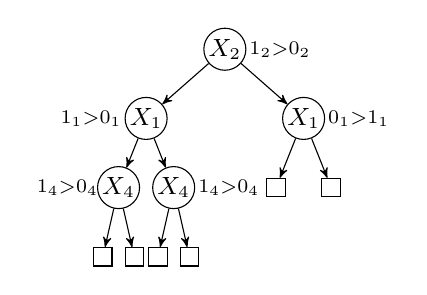
\begin{tikzpicture}[->,>=stealth',
	    level 1/.style={sibling distance=2cm, level distance=25pt},
			level 2/.style={sibling distance=0.7cm, level distance=25pt},
			level 3/.style={sibling distance=0.4cm, level distance=25pt}]
	    \node [main node,inner sep=0.5pt,label={[xshift=0.7cm, yshift=-0.5cm]$\scriptstyle 1_2>0_2$}] (1){$X_2$}
	      child {node [main node,inner sep=0.5pt,label={[xshift=-0.7cm, yshift=-0.5cm]$\scriptstyle 1_1>0_1$}] (3) {$X_1$}
	      	child {node [main node,inner sep=0.5pt,label={[xshift=-0.65cm, yshift=-0.5cm]$\scriptstyle 1_4>0_4$}] (7) {$X_4$}
	      		child {node [rectangle,draw] (8) {}}
	      		child {node [rectangle,draw] (9) {}}
					}
	      	child {node [main node,inner sep=0.5pt,label={[xshift=0.7cm, yshift=-0.5cm]$\scriptstyle 1_4>0_4$}] (10) {$X_4$}
	      		child {node [rectangle,draw] (11) {}}
	      		child {node [rectangle,draw] (12) {}}
					}
				}
	      child {node [main node,inner sep=0.5pt,label={[xshift=0.7cm, yshift=-0.5cm]$\scriptstyle 0_1>1_1$}] (6) {$X_1$}
	    		child {node [rectangle,draw] (4) {}}
	    		child {node [rectangle,draw] (5) {}}
	      };
	  \end{tikzpicture}
		\caption{Collapsible PLP-tree \label{fig:UICP_PLPT_full}}
	\end{subfigure}%
  \begin{subfigure}[b]{0.45\textwidth}
		\centering
	  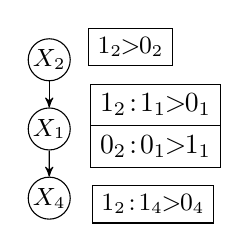
\begin{tikzpicture}[->,>=stealth',
	    level/.style={sibling distance=2cm/#1, level distance=25pt}]
	    \node [main node,inner sep=0.5pt] (1){$X_2$}
	      child {node [main node,inner sep=0.5pt] (2) {$X_1$}
	      	child {node [main node,inner sep=0.5pt] (3) {$X_4$} {}
							child {node [rectangle,draw] (4) at (1.7,2.8) {$1_2\!\!>\!\!0_2$} edge from parent[draw=none]}
							child {node [rectangle split, rectangle split parts=2,draw] (5) at (1.35,1.8)
								{$1_2\!:\!1_1\!\!>\!\!0_1$ \nodepart{second} $0_2\!:\!0_1\!\!>\!\!1_1$} edge from parent[draw=none]}
							child {node [rectangle,draw] (6) at (0.65,0.8) 
								{$1_2\!:\!1_4\!\!>\!\!0_4$} edge from parent[draw=none]}
					}
	      };
	  \end{tikzpicture}
		\caption{UI-CP PLP-tree \label{fig:UICP_PLPT_compact}}
	\end{subfigure}\\
  \begin{subfigure}[b]{0.45\textwidth}
		\centering
	  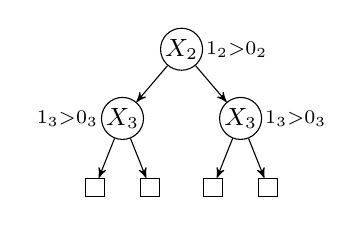
\begin{tikzpicture}[->,>=stealth',
	    level 1/.style={sibling distance=1.5cm, level distance=25pt},
			level 2/.style={sibling distance=0.7cm, level distance=25pt}]
	    \node [main node,inner sep=0.5pt,label={[xshift=0.7cm, yshift=-0.5cm]$\scriptstyle 1_2>0_2$}] (1){$X_2$}
	      child {node [main node,inner sep=0.5pt,label={[xshift=-0.7cm, yshift=-0.5cm]$\scriptstyle 1_3>0_3$}] (3) {$X_3$}
	    		child {node [rectangle,draw] (4) {}}
	    		child {node [rectangle,draw] (5) {}}
				}
	      child {node [main node,inner sep=0.5pt,label={[xshift=0.7cm, yshift=-0.5cm]$\scriptstyle 1_3>0_3$}] (6) {$X_3$}
	      		child {node [rectangle,draw] (8) {}}
	      		child {node [rectangle,draw] (9) {}}
	      };
	  \end{tikzpicture}
		\vspace{-0.1cm}
		\caption{Collapsible PLP-tree \label{fig:UIUP_PLPT_full}}
	\end{subfigure}%
  \begin{subfigure}[b]{0.45\textwidth}
		\centering
	  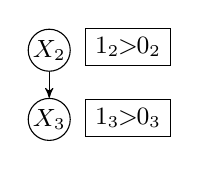
\begin{tikzpicture}[->,>=stealth',
	    level/.style={sibling distance=2cm/#1, level distance=25pt}]
	    \node [main node,inner sep=0.5pt] (1){$X_2$}
	      child {node [main node,inner sep=0.5pt] (2) {$X_3$}
							child {node [rectangle,draw] (4) at (1.5,1.8) {$1_2\!\!>\!\!0_2$} edge from parent[draw=none]}
							child {node [rectangle,draw] (5) at (0.5,0.9) {$1_3\!\!>\!\!0_3$} edge from parent[draw=none]}
	      };
	  \end{tikzpicture}
		\vspace{-0.2cm}
		\caption{UI-UP PLP-tree \label{fig:UIUP_PLPT_compact}}
	\end{subfigure}\\
  \begin{subfigure}[b]{0.45\textwidth}
		\centering
	  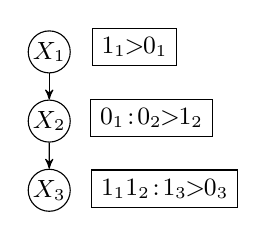
\begin{tikzpicture}[->,>=stealth',
	    level/.style={sibling distance=2cm/#1, level distance=25pt}]
	    \node [main node,inner sep=0.5pt] (1){$X_1$}
	      child {node [main node,inner sep=0.5pt] (2) {$X_2$}
	      	child {node [main node,inner sep=0.5pt] (3) {$X_3$}
							child {node [rectangle,draw] (4) at (1.75,2.7) {$1_1\!\!>\!\!0_1$} edge from parent[draw=none]}
							child {node [rectangle,draw] (5) at (1.3,1.8) {$0_1\!:\!0_2\!\!>\!\!1_2$} edge from parent[draw=none]}
							child {node [rectangle,draw] (6) at (0.8,0.9) {$1_11_2\!:\!1_3\!\!>\!\!0_3$} edge from parent[draw=none]}
					}
	      };
	  \end{tikzpicture}
		\vspace{-0.3cm}
		\caption{Invalid UI-CP PLP-tree \label{fig:invalid_UICP}}
	\end{subfigure}%
  \begin{subfigure}[b]{0.45\textwidth}
		\centering
	  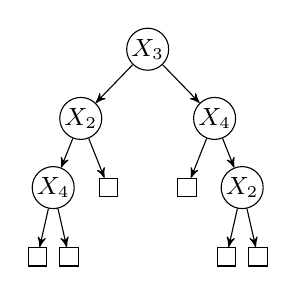
\begin{tikzpicture}[->,>=stealth',
	    level 1/.style={sibling distance=1.7cm, level distance=25pt},
			level 2/.style={sibling distance=0.7cm, level distance=25pt},
			level 3/.style={sibling distance=0.4cm, level distance=25pt}]
	    \node [main node,inner sep=0.5pt] (1){$X_3$}
	      child {node [main node,inner sep=0.5pt] (2) {$X_2$}
	    		child {node [main node,inner sep=0.5pt] (3) {$X_4$}
	      		child {node [rectangle,draw] (4) {}}
	      		child {node [rectangle,draw] (5) {}}
					}
	    		child {node [rectangle,draw] (6) {}}
				}
	      child {node [main node,inner sep=0.5pt] (7) {$X_4$}
	      	child {node [rectangle,draw] (8) {}}
	      	child {node [main node,inner sep=0.5pt] (9) {$X_2$}
	      		child {node [rectangle,draw] (10) {}}
	      		child {node [rectangle,draw] (11) {}}
					}
	      };
	  \end{tikzpicture}
		\caption{CI-FP PLP-tree \label{fig:noncoll_PLPT}}
	\end{subfigure}
  \caption{PLP-trees over the car domain}
  \label{fig:PLPTree}
\end{figure}


\vspace{-0.1cm}
\subsection{Classification of PLP-Trees}

\vspace{-0.1cm}
In the worst case, the size of a PLP-tree is exponential in the number of 
attributes in $\cI$. However, some PLP-trees have a special structure that
allows us to ``collapse'' them and obtain more compact 
representations. This yields a natural classification of PLP-trees, which
we describe below.

%Let $R$ be a sequence of attributes from $\cI$. By $\hat{R}$ we denote the
%set of attributes appearing in $R$. 
Let $R \subseteq \cI$ be the set of attributes that appear in a PLP-tree $T$. We say that $T$ is
\tit{collapsible} if there is a permutation $\hat{R}$ of elements in
$R$ such that for every path in $T$ from the root to a leaf, attributes 
that label nodes on that path appear in the same order in which they 
appear in $\hat{R}$. 

If a PLP-tree $T$ is collapsible, we can represent $T$ by a single path
of nodes labeled with attributes according to the order in which they occur
in $\hat{R}$, 
%(where $\hat{R}$ is the permutation of the set $R$ of attributes in $T$),
where a node labeled with an attribute $X_i$ is also assigned a
\tit{partial conditional preference table} (PCPT) that specifies 
preferences on $X_i$, conditioned on values of ancestor attributes in the path.
These tables make up for the lost structure of $T$ as different ways in 
which ancestor attributes evaluate correspond to different locations 
in the original tree $T$. 
Moreover, missing entries in PCPT of $X_i$ imply equivalence (or indifference) between values of $X_i$
under conditions that do not appear in the PCPT.
Clearly, the PLP-tree in \figref{UICP_PLPT_full} is collapsible, and can
be represented compactly as a single-path tree with nodes labeled by 
attributes in the permutation and PCPTs (cf. \figref{UICP_PLPT_compact}).
Such a collapsed path labeled by attributes is sometimes denoted as
a sequence of attributes in $\hat{R}$ connected by $\triangleright$, e.g.,
$X_2\triangleright X_3\triangleright X_1$ for the path in \figref{UICP_PLPT_compact}.

Collapsible PLP-trees represented by a single path of nodes 
will be referred to as \emph{unconditional importance} trees or $\UI$ 
trees, for short. The name reflects the fact that the order in which 
we consider attributes when seeking the rank of an outcome is always the 
same (not conditioned on the values of ancestor attributes of higher importance).

Let $L$ be a collapsible PLP-tree.
If for every path in $L$ the order of attributes labeling the path is exactly $\hat{R}$,
and $L$ has the same preference $1>0$ on \emph{every} node,
then every PCPT in the collapsed tree contains the same preference $1>0$,
no matter the evaluation of the ancestor attributes.
Thus, every PCPT in the collapsed form can be simplified to a single \emph{fixed} preference $1>0$,
a shorthand for its full-sized counterpart.
We call the resulting
collapsed tree a $\UI$ tree with \emph{fixed preferences}, or a $\UI$-$\FP$ PLP-tree.

A similar simplification is possible if every path in $L$ has the same ordering of attributes
which again is exactly $\hat{R}$, and
for every attribute $X_i$ all nodes in $L$ labeled with $X_i$ have the same
preference on values of $X_i$ (either $1_i>0_i$ or $0_i>1_i$).
Such collapsed 
trees are called $\UI$-$\UP$ PLP-trees, with $\UP$ standing for \emph{unconditional 
preference}. As an example, the $\UI$-$\UP$ tree in \figref{UIUP_PLPT_compact}
is the collapsed representation of the collapsible tree in \figref{UIUP_PLPT_full}.

In all other cases, we refer to collapsed PLP-trees as $\UI$-$\CP$ PLP-trees, 
with $\CP$ standing for \emph{conditional preference}. If preferences on 
an attribute in such a tree depend in an essential way on all preceding 
attributes, there is no real saving in the size of representation (instead 
of an exponential PLP-tree we have a small tree but with preference 
tables that are of exponential size). However, if the preference on an 
attribute depends only on a few higher importance attributes say, never more than 
one or two (or, more generally, never more than some fixed bound $b$), 
the collapsed representation is significantly smaller.

As an aside, we note that not every path of nodes labeled with attributes
and PCPTs is a $\UI$ tree. An example is given in \figref{invalid_UICP}.
Indeed, one can see that there is no PLP-tree that would collapse to 
it. There is a simple condition 
characterizing paths with nodes labeled with attributes and PCPTs that
are valid $\UI$ trees. This matter is not essential to our discussion later 
on and we will not discuss it further here.  
 
When a PLP-tree is not collapsible, the importance of an attribute depends
on where it is located in the tree. We will refer to such PLP-trees as
\tit{conditional importance} trees or $\CI$ trees.

Let $T$ be a $\CI$ PLP-tree.
We call $T$ a $\CI$-$\FP$ tree if every non-leaf node in $T$
is labeled by an attribute with preference $1>0$.
An example of a $\CI$-$\FP$ PLP-tree is shown in \figref{noncoll_PLPT}, where
preferences on each non-leaf node are $1>0$ and hence omitted.
If, for every attribute $X_i$, all nodes in $T$ labeled with $X_i$
have the same preference ($1_i>0_i$ or $0_i>1_i$) on $X_i$, we say $T$ is
a $\CI$-$\UP$ PLP-tree.  
All other non-collapsible PLP-trees are called $\CI$-$\CP$ PLP-trees.
%As mentioned above, the size of $\CI$-$\CP$ trees in the worst case
%could be too large due to the binary tree structure.
%However, if the depth of the tree or the number of paths is bounded 
%by some constant, the size of the model will be substantially reduced.


\section{Passive Learning}

An \tit{example} is a tuple $(\alpha, \beta, v)$, where $\alpha$ and 
$\beta$ are two \emph{distinct} outcomes from combinatorial domain 
$\cX$ over a set $\cI=\{X_1,\ldots,
X_p\}$ of binary attributes, and $v \in \{0,1\}$. An example $(\alpha,\beta,1)$
states that $\alpha$ is strictly preferred to $\beta$ ($\alpha \succ \beta$).
Similarly, an example $(\alpha,\beta,0)$ states that $\alpha$ and $\beta$ 
are equivalent ($\alpha\approx\beta$). Let $\cE=\{e_1,\ldots,e_m\}$ be a set 
of examples over $\cI$, with $e_i=(\alpha_i,\beta_i,v_i)$. We set 
$\cE^{\approx}= \{e_i \in \cE: v_i=0\}$, and $\cE^{\succ}= \{e_i \in \cE: 
v_i =1\}$. 
In the following, we denote by $p$ and $m$ the number of attributes and the number of
examples, respectively.

For a PLP-tree $T$ in full representation we denote by $|T|$ the size of $T$, 
that is, the number of nodes in $T$. If $T$ stands for a $\UI$ tree, we write $|T|$ for
the size of $T$ measured by the total size of preference tables associated
with attributes in $T$. The size of a preference table is the total size of
preferences in it, each preference measured as the number of values in the condition
plus $1$ for the preferred value in the domain of the attribute.
In particular, the sizes of $\UI$-$\FP$ and $\UI$-$\UP$ trees are
given by the number of nodes on the path. 

A PLP-tree $T$ \tit{satisfies} an example $e$ if $T$ orders the two 
outcomes of $e$ in the same way as they are ordered in $e$. Otherwise,
$T$ \tit{falsifies} $e$. Formally, $T$ \tit{satisfies} $e=(\alpha,\beta,1)$
if $\alpha \succ_T \beta$, and $T$ \tit{satisfies} $e=(\alpha,\beta,0)$ if
$\alpha \approx_T \beta$. We say $T$ is \tit{consistent} with a set $\cE$ 
of examples if $T$ satisfies every example in $\cE$.

In this work, we study the following passive learning problems for PLP-trees 
of all types we introduced.
\begin{definition}
Consistent-learning (\tsc{ConsLearn}): given an example set $\cE$, decide 
whether there exists a PLP-tree $T$ (of a particular type) such that $T$ 
is consistent with $\cE$.
\end{definition}

\begin{definition}
Small-learning (\tsc{SmallLearn}): given an example set $\cE$
and a positive integer $l$ ($l \leq |\cE|$), decide whether there 
exists a PLP-tree $T$ (of a particular type) such that $T$ is consistent 
with $\cE$ and $|T| \leq l$.
\end{definition}

\begin{definition}
Maximal-learning (\tsc{MaxLearn}): given an example set $\cE$ and a 
positive integer $k$ ($k \leq m$), decide whether there exists a PLP-tree 
$T$ (of a particular type) such that $T$ satisfies at least $k$ examples 
in $\cE$.
\end{definition}


\section{Learning UI PLP-trees}
In this section, we study the passive learning problems for collapsible 
PLP-trees in their collapsed representations as $\UI$-$\FP$, $\UI$-$\UP$ and
$\UI$-$\CP$ trees.


\vspace{-0.1cm}
\subsection{The \tsc{ConsLearn} Problem}
\vspace{-0.1cm}
%Since how hard is the problem in the setting of $\UI$-$\CP$ trees remains open
%at the time of this paper, we will study it in the future and
%in this work we focus on the other two $\UI$ cases for the \tsc{ConsLearn} problem.

The \tsc{ConsLearn} problem is in the class P for $\UI$-$\FP$ and
$\UI$-$\UP$ trees. To show it, we present a general template of an 
algorithm that learns a $\UI$ tree. Next, for each of the classes 
$\UI$-$\FP$ and $\UI$-$\UP$, we specialize the template to a 
polynomial-time algorithm.

The template algorithm is shown as \algref{learnUI}. The 
input consists of a set $\cE$ of examples and a set $\cI$ of attributes 
from which node labels can be selected. Throughout the execution, the 
algorithm maintains a set $S$ of unused attributes, initialized to $\cI$, 
and a set of examples that are not yet ordered by the tree constructed 
so far.

If the set of strict examples is empty, the algorithm returns an empty tree. 
Otherwise, the algorithm identifies the set $\AI(\cE,S)$ of attributes in 
$S$ that are \emph{available} for selection as the label for the next 
node. If that set is empty, the algorithm terminates with failure. If
not, an attribute, say $X_l$, is selected from $\AI(\cE,S)$, and a PCPT for
that attribute is constructed. Then the sets of examples not ordered yet 
and of attributes not used yet are updated, and the steps repeat.  

\begin{algorithm}[ht]
\KwIn{$\cE$ and $S=\cI$}
\KwOut{A sequence $T$ of attributes from $\cI$ and PCPTs that define
a $\UI$ tree consistent with $\cE$, or FAILURE if such a tree does not 
exist}

	$T \leftarrow \mbox{empty sequence}$\;
	\While{$\cE^\succ \neq \emptyset$}{
        Construct $\AI(\cE,S)$\;
        \If{$\AI(\cE,S)=\emptyset$}{
                \Return FAILURE\;
        }
        $X_l \leftarrow \mbox{an element from $\AI(\cE,S)$}$\;
	Construct $\PCPT(X_l)$\; 
	$T \leftarrow T, (X_l, \PCPT(X_l))$\;
        $\cE \leftarrow \cE \backslash \{e \in \cE^\succ: e$ is decided on $X_l\}$\;
        $S \leftarrow S \backslash \{X_l\}$\;
	}
        \Return $T$\;
\caption{Procedure \tit{learnUI} that learns a UI tree 
\label{alg:learnUI}}
\end{algorithm}

To obtain a learning algorithm for a particular class of $\UI$ trees
($\UI$-$\FP$ or $\UI$-$\UP$) we need to specify the notion 
of an available attribute (needed for line 3) and describe how to construct 
a partial conditional preference table (needed for line 8). 

To this end, let us define $\NEQ(\cE,S)$ to be the set of all attributes in
$S$ (where $S\subseteq \cI$) that incorrectly handle at least one equivalent example 
in $\cE^\approx$. That is, for an attribute $X\in S$ we have $X\in \NEQ(\cE,S)$
precisely when for some example $(\alpha,\beta,0)$ in $\cE$, $\alpha(X)\not=
\beta(X)$. Similarly, let us define $\EQ(\cE,S)$ to be the set of 
attributes in $S$ that do not order any of the strict examples in $\cE$. That 
is, for an attribute $X\in S$ we have $X\in \EQ(\cE,S)$ precisely when 
for every example $(\alpha,\beta,1)$ in $\cE$, $\alpha(X)= \beta(X)$.  

\noindent {\bf Fixed Preferences.}
For the problem of learning $\UI$-$\FP$ trees, we define $\AI(\cE,S)$ to
contain every attribute $X\notin \NEQ(\cE,S)$ such that\\ 
(1) \ for every $(\alpha,\beta,1) \in \cE^\succ$, $\alpha(X) 
\geq \beta(X)$.

\begin{prop}
\label{prop:1}
{\it If there is a $\UI$-$\FP$ tree consistent with all examples in $\cE$ and 
using only attributes from $S$ as labels, then an attribute $X\in S$ is a top node
of some such tree if and only if $X\in \AI(\cE,S)$.}
\end{prop}
\begin{proof}
Let $T$ be a $\UI$ tree consistent with $\cE$ and having only attributes from 
$S$ as labels. Let $X$ be the attribute labeling the top node of $T$. Clearly,
$X\notin \NEQ(\cE,S)$, as otherwise, $T$ would strictly order two outcomes
$\alpha$ and $\beta$ such that $(\alpha,\beta,0)\in \cE^\approx$. To prove
condition (1), let us consider any example $(\alpha,\beta,1)\in \cE^\succ$. 
Since $T$ is consistent with $(\alpha,\beta,1)$, $\alpha(X)\geq\beta(X)$. 
Consequently, $X\in \AI(\cE,S)$.

Conversely, let $X\in \AI(\cE,S)$ and let $T$ be a $\UI$-$\FP$ tree 
consistent with all examples in $\cE$ and using only attributes from $S$ as 
labels (such a tree exists by assumption). If $X$ labels the top node in 
$T$, we are done. Otherwise, let $T'$ be a tree obtained from $T$ by 
adding at the top of $T$ another node, labeling it with $X$ and removing
from $T$ the node labeled by $X$, if such a node exists. By the definition
of $\AI(\cE,S)$ we have that $X\notin\NEQ(\cE,S)$ and that condition (1) 
holds for $X$. Using these properties, we see that $T'$ is also 
a $\UI$-$\FP$ 
tree consistent with all examples in $\cE$. Since the top node of $T'$
is labeled by $X$, the assertion follows. 
\end{proof}

We now specialize \algref{learnUI} by using in line 3 the 
definition of $\AI(\cE,S)$ given above and by setting each $\PCPT(X_l)$ 
to the fixed unconditional preference $1_l>0_l$. Proposition \ref{prop:1}
directly implies the correctness of this version of \algref{learnUI}.

\begin{thm}
Let $\cE$ be a set of examples over a set $\cI$ of binary attributes.
\algref{learnUI} adjusted as described above terminates and outputs
a sequence $T$ representing a $\UI$-$\FP$ tree consistent with $\cE$ if
and only if such a tree exists.
\end{thm}

We note that attributes in $\NEQ(\cE,S)$ are never used when constructing
$\AI(\cE,S)$. Thus, in the case of $\UI$-$\FP$ trees, $S$ could be
initialized to $\cI\setminus\NEQ(\cE,\cI)$. In addition, if an attribute
selected for the label of the top node belongs to $\EQ(\cE^\succ, S)$,
it does not in fact decide any of the strict examples in $\cE$ and can be
dropped. The resulting tree is also consistent with all the examples. 
Thus, the definition of $\AI(\cE,S)$ can be refined by requiring one more
condition: $X \not \in \EQ(\cE^\succ, S)$. That change does not affect 
the correctness of the algorithm but eliminates a possibility of generating
trees with ``redundant'' levels.


\noindent {\bf Unconditional Preferences.}
The case of learning $\UI$-$\UP$ trees is very similar to the 
previous one. Specifically, we define $\AI(\cE,S)$ to contain an attribute 
$X\in S$ precisely when $X\notin\NEQ(\cE,S)$ and

\noindent 
(2) \ for every $(\alpha,\beta,1) \in \cE^\succ$, $\alpha(X) \geq 
\beta(X)$, or for every $(\alpha,\beta,1) \in \cE^\succ$, $\alpha(X) \leq \beta(X)$.

We obtain an algorithm learning $\UI$-$\UP$ trees by using in line 3
the present definition of $\AI(\cE,S)$. In line 8, we take for 
$\PCPT(X_l)$ either $1_l>0_l$ or $0_l>1_l$ (depending on which of the two
cases in (2) holds for $X_l$).

The correctness of this algorithm follows from a property similar to
that in \propref{1}.

As in the previous case, here too $S$ could be initialized to $\cI \setminus
\NEQ$, and the condition $X\not\in \EQ(\cE^\succ,S)$ could be added to the 
definition of $\AI(\cE,S)$. 

\noindent {\bf Conditional Preferences.} 
The problem is in NP because, if a $\UI$-$\CP$
tree consistent with $\cE$ exists (\emph{a priori},
it does not have to have size polynomial in the size of $\cE$), then another
such tree of size polynomial in the size of $\cE$ exists, as well.
We conjecture that the general problem of
learning $\UI$-$\CP$ trees is, in fact, NP-complete. 
As we have only partial results 
for this case, the study of the $\UI$-$\CP$ tree learning will be the subject
of future work. 


\vspace{-0.1cm}
\subsection{The \tsc{SmallLearn} Problem}

\vspace{-0.1cm}
\algref{learnUI} produces a $\UI$ PLP-tree consistent with $\cE$, if one exists.
In many cases, it is desirable to compute a small, sometimes even the smallest, 
representation consistent with $\cE$.
We show that these problems for $\UI$ trees are NP-hard.

\begin{thm}
\label{thm:UIFP_smallest_decision}
	The \tsc{SmallLearn} problem is NP-complete for each class of $\{\UI\} \times \{\FP,\UP,\CP\}$.
\end{thm}
\begin{proof}
	We present the proof only in the case of $\UI$-$\FP$. The argument in other cases 
	($\UI$-$\UP$ and $\UI$-$\CP$) is similar.

	(Membership) One can guess a $\UI$-$\FP$ PLP-tree $T$ in linear time, and verify in polynomial time that 
	$T$ has at most $l$ attributes and satisfies every example in $\cE$.

	(Hardness) We present a polynomial-time reduction from the
	\tit{hitting set problem} (HSP), which is NP-complete 
    \cite{Garey:1979}. To recall, in HSP we are given a finite
		set $U=\{a_1,\ldots,a_n\}$, a collection $C=\{S_1,\ldots,
    S_d\}$ of subsets of $U$ with $\bigcup_{S_i \in C} S_i = U$,
    and a positive integer $k \leq n$, and the problem is to
    decide whether $U$ has a hitting set $U'$ such that $|U'|\leq k$ 
    ($U'\subseteq U$ is a \emph{hitting} set for $C$ if 
		$U' \cap S_i \not = \emptyset$ for all $S_i \in C$).
	Given an instance of HSP, we construct an instance of our problem as follows.

	\noindent 1. $\cI=\{X_i: a_i \in U\}$ (thus, $p=n$).

	\noindent 2. $\cE=\{(\tbf{s}_i, \tbf{0},1): S_i \in C\}$, where
	$\tbf{s}_i$ is a $p$-bit vector such that $\tbf{s}_i[j]=1 \Leftrightarrow a_j \in S_i$
	and $\tbf{s}_i[j]=0 \Leftrightarrow a_j \not \in S_i$ ($1 \leq j \leq p$), 
	and $\tbf{0}$ is a $p$-bit vector of all $0$'s (thus, $m=d$).

	\noindent 3. We set $l=k$.

	We need to show that $U$ has a hitting set of size at most $k$ if and only if
	there exists a $\UI$-$\FP$ PLP-tree of size at most $l$ consistent with $\cE$.

\smallskip
\noindent
	($\Rightarrow$) Assume $U$ has a hitting set $U'$ of size $k$.
	Let $U'$ be $\{a_{j_1},\ldots,a_{j_k}\}$.
	Define a $\UI$-$\FP$ PLP-tree $L=X_{j_1} \triangleright \ldots \triangleright X_{j_k}$.
	We show that $L$ is consistent with $\cE$.
	Let $e=(\alpha_e,\beta_e,1)$ be an arbitrary example in $\cE$, where
	$\alpha_e=\tbf{s}_i$ and $\beta_e=\tbf{0}$.
	Since $U'$ is a hitting set, %for every set $S_i\in C$ 
        there exists $r$, $1 \leq r \leq k$, 
	%$a_{j_r}$ ($1 \leq r \leq k$) 
        such that $a_{j_r} \in S_i$.
	Thus, %for $\alpha_e$ 
        there exists $r$, $1 \leq r \leq k$, %$X_{j_r}$ ($1 \leq r \leq k$)
	such that $\alpha_e(X_{j_r})=1$.
	Let $r$ be the smallest with this property. 
	%Among these attributes $X_{j_r}$ let $X_j$ be the top-ranked one.
	It is clear that $e$ is decided at $X_{j_r}$; thus, we have 
	$\alpha_e \succ_L \beta_e$.

\smallskip
\noindent
	($\Leftarrow$) Assume there is a $\UI$-$\FP$ PLP-tree $L$ of $l$ attributes in
	$\cI$ such that $L$ is consistent with $\cE$. Moreover, we assume
	$L=X_{j_1} \triangleright \ldots \triangleright X_{j_l}$.
	Let $U'=\{a_{j_1}, \ldots,a_{j_l}\}$.
	We show by means of contradiction.  Assume that $U'$ is not a hitting set.
	That is, there exists a set $S_i \in C$ such that
	$U' \cap S_i = \emptyset$.
	Then, there exists an example $e=(\alpha_e,\beta_e,1)$, where $\alpha_e=\tbf{s}_i$ 
	and $\beta_e=\tbf{0}$, such that $\alpha_e \approx_L \beta_e$ because
	none of the attributes $\{X_i:\alpha_e(X_i)=1\}$ show up in $L$. This is
	a contradiction! Thus, $U'$ is a hitting set.
\end{proof}

\begin{cor}
\label{cor:UIFP_smallest}
	Given a set $\cE$ of examples $\{e_1,\ldots,e_m\}$ over $\cI=\{X_1,\ldots,X_p\}$,
	finding the smallest PLP-tree in each class of $\{\UI\} \times \{\FP,\UP,\CP\}$ 
	consistent with $\cE$ is NP-hard.
\end{cor}

Consequently, it is important to study fast heuristics that aim at
approximating trees of optimal size. 
Here, we propose a greedy heuristic for \algref{learnUI}.
In every iteration the heuristic selects the attribute $X_l \in \AI(\cE,S)$ that
decides the most examples in $\cE^\succ$.
However, for some dataset the resulting greedy algorithm does not perform 
well: the ratio of the size of the tree computed by our algorithm 
to the size of the optimal sequence may be as large as $\Omega(p)$.
To see this, we consider the following input.

\begin{framed}
	\vspace{-0.2cm}
	\noindent $(1_10_20_30_4,0_10_20_30_4,1)$\\
	$(1_11_20_30_4,0_10_20_30_4,1)$\\
	$(1_10_21_30_4,0_10_20_30_4,1)$\\
	$(0_10_20_31_4,1_10_20_30_4,1)$
	\vspace{-0.2cm}
\end{framed}

For each class of $\{\UI\} \times \{\FP,\UP\}$, \algref{learnUI} in the worst 
case computes $X_2 \triangleright X_3 \triangleright X_4 \triangleright X_1$,
whereas the optimal tree is $X_4 \triangleright X_1$ (with
the PCPTs omitted as they contain only one preference and so, they do not
change the asymptotic size of the tree). This example generalizes to the
arbitrary number $p$ of attributes. Thus, the greedy algorithm to learn small
$\UI$ trees is no better than any other algorithm in 
the worst case.

Approximating HSP has been extensively studied over the last decades.
It has been shown \cite{lund1994hardness} that, unless $\NP \subset \DTIME(n^{\poly \log n})$,
HSP cannot be approximated 
in polynomial time within factor of $c \log n$, where $0<c<\frac{1}{4}$ and
$n$ is the number of elements in the input. The reduction we used above
shows that this result
carries over to our problem.
\begin{thm}
\label{thm:UI_smallest_approx}
	Unless $\NP \subset \DTIME(n^{\poly \log n})$,
	the problem of finding the smallest PLP-tree in each class of $\{\UI\} \times \{\FP,\UP,\CP\}$ 
	consistent with $\cE$ cannot be approximated 
	in polynomial time within factor of $c \log p$, where $0<c<\frac{1}{4}$.
\end{thm}
It is an open problem whether this result can be strengthened to a factor 
linear in $p$ (cf. the example for the worst-case behavior of our simple 
greedy heuristic).


\vspace{-0.1cm}
\subsection{The \tsc{MaxLearn} Problem}

\vspace{-0.1cm}
When there is no $\UI$ PLP-tree consistent with the set of all examples,
it may be useful to learn a $\UI$ PLP-tree satisfying as many examples 
as possible. We show this problem is in fact NP-hard for all three 
classes of $\UI$ trees.

\begin{thm}
\label{thm:UIFP_least_decision}
The \tsc{MaxLearn} problem is NP-complete for each class of $\{\UI\} \times \{\FP,\UP,\CP\}$.
\end{thm}
\begin{proof}
The problem is in NP. This is evident for the case
of $\UI$-$\FP$ and $\UI$-$\UP$ trees. If $\cE$ is a given set of examples,
and $k$ a required lower bound on the number of examples that are to be 
correctly ordered, then witness trees in these classes (trees that correctly 
order at least $k$ examples in $\cE$) have size polynomial in the size of 
$\cE$. Thus, verification can be performed in polynomial time. 
For the case of $\UI$-$\CP$ trees, if there is a $\UI$-$\CP$
tree correctly ordering at least $k$ examples in $\cE$, then there exists
such tree of size polynomial in $|\cE|$.

The hardness part follows from the proof in the setting of learning 
lexicographic strategies \cite{schmitt2006complexity}, adapted to the case 
of $\UI$ PLP-trees.
\end{proof}

\begin{cor}
\label{cor:UIFP_least}
Given a set $\cE$ of examples $\{e_1,\ldots,e_m\}$ over 
$\cI=\{X_1,\ldots,X_p\}$, finding a PLP-tree in each class of $\{\UI\} \times \{\FP,\UP,\CP\}$ 
satisfying the maximum number of examples in $\cE$ is NP-hard.
\end{cor}

\section{Learning CI PLP-trees}
Finally, we present results on the passive learning problems for 
PLP-trees in classes $\{\CI\} \times \{\FP,\UP,\CP\}$. We recall that these
trees assume full (non-collapsed) representation.


\vspace{-0.1cm}
\subsection{The \tsc{ConsLearn} Problem}

\vspace{-0.1cm}
We first show that the \tsc{ConsLearn} problem for class $\CI$-$\UP$ is 
NP-complete. We then propose polynomial-time algorithms to solve the 
\tsc{ConsLearn} problem
%so as to show that the problem is in class P, 
for the classes $\CI$-$\FP$ and $\CI$-$\CP$.

\begin{thm}
\label{thm:passlearn_CIUP}
	The \tsc{ConsLearn} problem is NP-complete for class $\CI$-$\UP$.
\end{thm}
\begin{proof}
The problem is in NP because the size of a witness, 
a $\CI$-$\UP$ PLP-tree consistent with $\cE$, is bounded by $|\cE|$ (
if a $\CI$-$\UP$ tree consistent with $\cE$ exists, then it can
be modified to a tree of size no larger than $O(|\cE|)$).
	Hardness follows from the proof by Booth et al. \shortcite{booth:learningLP} showing 
	\tsc{ConsLearn} is NP-hard in the setting of LP-trees.
\end{proof}

For the two other classes of trees, the problem is in P. This is demonstrated 
by polynomial-time \algref{recur_learnCI} adjusted for both classes.

\begin{algorithm}[ht]
\KwIn{$\cE$, $S=\cI$, and $t$: an unlabeled node}
\KwOut{A CI PLP-tree over $S$ consistent with $\cE$, or FAILURE}
	\If{$\cE^\succ = \emptyset$}{
		Label $t$ as a leaf and \Return\;
	}
	Construct $\AI(\cE,S)$\;
	\If{$\AI(\cE,S)=\emptyset$}{
		\Return FAILURE and terminate\;
	}
	Label $t$ with tuple $(X_l,x_l)$ where $X_l$ is from $\AI(\cE,S)$, 
		and $x_l$ is the preferred value on $X_l$\;
	$\cE \leftarrow \cE \backslash \{e \in \cE^\succ: e$ is decided on $X_l\}$\;
	$S \leftarrow S \backslash \{X_l\}$\;
	Create two edges $u_l,u_r$ and two unlabeled nodes $t_l,t_r$ such that $u_l=\langle t,t_l\rangle$
		and $u_r=\langle t,t_r\rangle$\;
	$\cE_l \leftarrow \{e\in \cE: \alpha_e(X_j)=\beta_e(X_j)=x_l\}$\;
	$\cE_r \leftarrow \{e\in \cE: \alpha_e(X_j)=\beta_e(X_j)=\overline{x_l}\}$\;
	$\mathit{learnCI}(\cE_l,S,t_l)$\;
	$\mathit{learnCI}(\cE_r,S,t_r)$\;

\caption{The recursive procedure \tit{learnCI} that learns a CI PLP-tree \label{alg:recur_learnCI}}
\end{algorithm}

\noindent {\bf Fixed Preference.}
For class $\CI$-$\FP$, we define $\AI(\cE,S)$ to contain attribute 
$X\notin \NEQ(\cE,S)$ if\\
(3) \ for every $(\alpha,\beta,1) \in \cE^\succ$,  $\alpha(X) \geq \beta(X)$.

\begin{prop}
\label{prop:2}
{\it If there is a $\CI$-$\FP$ tree consistent with all examples in $\cE$ and 
using only attributes from $S$ as labels, then an attribute $X\in S$ is a top node
of some such tree if and only if $X\in \AI(\cE,S)$.}
\end{prop}
\begin{proof}
	It is clear that if there exists a $\CI$-$\FP$ PLP-tree consistent with $\cE$
	and only using attributes from $S$ as labels, then the fact that
	$X \in S$ labels the root of some such tree implies $X \in \AI(\cE,S)$.

	Now we show the other direction.
	Let $T$ be the $\CI$-$\FP$ tree over a subset of $S$ consistent 
	with $\cE$,
	$X$ be an attribute such that $X \in \AI(\cE,S)$.
	If $X$ is the root attribute in $T$, we are done.
	Otherwise, we construct a $\CI$-$\FP$ tree $T'$ by creating a root, 
	labeling it with $X$, and make one copy of $T$ the left subtree of $T'$
        ($T_l'$) and another, the right subtree of $T'$ ($T_r'$).
	For a node $t$ and a subtree $B$ in $T$, we write $t_l'$ and $B_l'$, 
	respectively, for the corresponding node and subtree in $T_l'$.
	We define $t_r'$ and $B_r'$ similarly. If $X$ does not appear in 
	$T$, we are done constructing $T'$; otherwise, we update $T'$ as 
	follows.

	\noindent 1). For every node $t\in T$ labeled by $X$ such that $t$ has two leaf children,
	we replace the subtrees rooted at $t_l'$ and $t_r'$ in $T_l'$ and $T_r'$ with leaves.

	\noindent 2). For every node $t \in T$ labeled by $X$ such that $t$ has one leaf child
	and a non-leaf subtree $B$, we replace the subtree rooted at $t_l'$ in $T_l'$ with $B_l'$,
	and the subtree rooted at $t_r'$ in $T_r'$ with a leaf,
	if $t \in T$ has a right leaf child; otherwise, we replace the subtree rooted at
	$t_l'$ in $T_l'$ with a leaf, and the subtree rooted at $t_r'$ in $T_r'$ with $B_r'$.

	\noindent 3). Every other node $t \in T$ labeled by $X$ has two non-leaf subtrees:
	left non-leaf subtree $\BL$ and right $\BR$.
	For every such node $t \in T$, we replace the subtree rooted at $t_l'$ in $T_l'$ with
	$\BL_l'$, and the subtree rooted at $t_r'$ in $T_r'$ with $\BR_r'$.

	As an example, this construction of $T'$ from $T$ is demonstrated in \figref{promote}.
	We see that this construction results in a $\CI$-$\CP$ tree consistent
	with $\cE$ and, clearly, it has its root labeled with $X$.
	Thus, the assertion follows.
\end{proof}

\begin{figure}
	\centering
  \begin{subfigure}[b]{0.45\textwidth}
		\centering
	  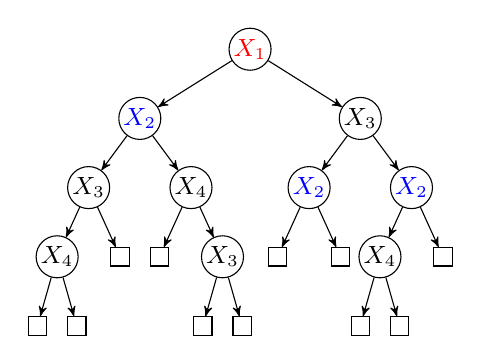
\begin{tikzpicture}[->,>=stealth',
		    level 1/.style={sibling distance=2.8cm, level distance=25pt},
		    level 2/.style={sibling distance=1.3cm, level distance=25pt},
				level 3/.style={sibling distance=0.8cm, level distance=25pt},
				level 4/.style={sibling distance=0.5cm, level distance=25pt}]
	    \node [main node,inner sep=0.5pt] (1){$\redtext{X_1}$}
	      child {node [main node,inner sep=0.5pt] (2) {$\bluetext{X_2}$}
	      	child {node [main node,inner sep=0.5pt] (3) {$X_3$} {}
		      	child {node [main node,inner sep=0.5pt] (4) {$X_4$}
		      		child {node [rectangle,draw] (5) {}}
		      		child {node [rectangle,draw] (6) {}}
						}
		      	child {node [rectangle,draw] (7) {}}
					}
	      	child {node [main node,inner sep=0.5pt] (8) {$X_4$} {}
		      	child {node [rectangle,draw] (9) {}}
		      	child {node [main node,inner sep=0.5pt] (10) {$X_3$}
		      		child {node [rectangle,draw] (11) {}}
		      		child {node [rectangle,draw] (12) {}}
						}
					}
	      }
	      child {node [main node,inner sep=0.5pt] (13) {$X_3$}
	      	child {node [main node,inner sep=0.5pt] (14) {$\bluetext{X_2}$} {}
		      	child {node [rectangle,draw] (15) {}}
		      	child {node [rectangle,draw] (16) {}}
					}
	      	child {node [main node,inner sep=0.5pt] (17) {$\bluetext{X_2}$} {}
		      	child {node [main node,inner sep=0.5pt] (18) {$X_4$}
		      		child {node [rectangle,draw] (19) {}}
		      		child {node [rectangle,draw] (20) {}}
						}
		      	child {node [rectangle,draw] (21) {}}
					}
				};
	  \end{tikzpicture}
		\caption{$T$ \label{fig:promote_T}}
	\end{subfigure}\\
  \begin{subfigure}[b]{0.45\textwidth}
		\centering
	  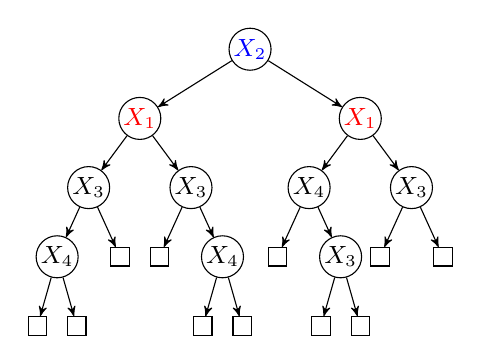
\begin{tikzpicture}[->,>=stealth',
		    level 1/.style={sibling distance=2.8cm, level distance=25pt},
		    level 2/.style={sibling distance=1.3cm, level distance=25pt},
				level 3/.style={sibling distance=0.8cm, level distance=25pt},
				level 4/.style={sibling distance=0.5cm, level distance=25pt}]
	    \node [main node,inner sep=0.5pt] (1){$\bluetext{X_2}$}
	      child {node [main node,inner sep=0.5pt] (2) {$\redtext{X_1}$}
	      	child {node [main node,inner sep=0.5pt] (3) {$X_3$} {}
		      	child {node [main node,inner sep=0.5pt] (4) {$X_4$}
		      		child {node [rectangle,draw] (5) {}}
		      		child {node [rectangle,draw] (6) {}}
						}
		      	child {node [rectangle,draw] (7) {}}
					}
	      	child {node [main node,inner sep=0.5pt] (8) {$X_3$} {}
		      	child {node [rectangle,draw] (9) {}}
		      	child {node [main node,inner sep=0.5pt] (10) {$X_4$}
		      		child {node [rectangle,draw] (11) {}}
		      		child {node [rectangle,draw] (12) {}}
						}
					}
	      }
	      child {node [main node,inner sep=0.5pt] (13) {$\redtext{X_1}$}
	      	child {node [main node,inner sep=0.5pt] (14) {$X_4$} {}
		      	child {node [rectangle,draw] (15) {}}
		      	child {node [main node,inner sep=0.5pt] (16) {$X_3$}
		      		child {node [rectangle,draw] (17) {}}
		      		child {node [rectangle,draw] (18) {}}
						}
					}
	      	child {node [main node,inner sep=0.5pt] (19) {$X_3$} {}
		      	child {node [rectangle,draw] (20) {}}
		      	child {node [rectangle,draw] (21) {}}
					}
				};
	  \end{tikzpicture}
		\caption{$T'$ \label{fig:promote_T_updated}}
	\end{subfigure}
	\caption{$X_2 \in \AI(\cE,S)$ is picked at the root \label{fig:promote}}
\end{figure}

\propref{2} clearly implies the correctness of \algref{recur_learnCI} with 
$\AI(\cE,S)$ defined as above for class $\CI$-$\FP$ and each $x_l \in 
(X_l,x_l)$ set to $1$.

\begin{thm}
Let $\cE$ be a set of examples over a set $\cI$ of binary attributes.
\algref{recur_learnCI} adjusted as described above terminates and outputs
a $\CI$-$\FP$ tree $T$ consistent with $\cE$ if
and only if such a tree exists.
\end{thm}


\noindent {\bf Conditional Preference.}
For class $\CI$-$\CP$, we define that $\AI(\cE,S)$ contains attribute $X \not \in \NEQ(\cE)$ if 

\noindent (4) \ for every $(\alpha,\beta,1) \in \cE^\succ$, $\alpha(X) \geq 
\beta(X)$, or for every $(\alpha,\beta,1) \in \cE^\succ$, $\alpha(X) \leq \beta(X)$.

We obtain an algorithm learning $\CI$-$\CP$ trees by using in line 4
the present definition of $\AI(\cE,S)$. In line 8, we take for 
$x_l$ either $1$ or $0$ (depending on which of the two
cases in (4) holds for $X_l$).
The correctness of this algorithm follows from a property similar to
that in \propref{2}.


\vspace{-0.1cm}
\subsection{The \tsc{SmallLearn} and \tsc{MaxLearn} Problems}

\vspace{-0.1cm}
We outline the results we have for this case. 
Both problems for the three $\CI$ classes are NP-complete. They are in 
NP since if a witness PLP-tree exists, one can modify it so that 
its size does not exceed the size of the input. Hardness of the 
\tsc{SmallLearn} problem for $\CI$ classes follows from the proof of 
\thmref{UIFP_smallest_decision}, whereas the hardness of the 
\tsc{MaxLearn} problem for $\CI$ cases follows from the proof 
by Schmitt and Martignon \shortcite{schmitt2006complexity}.


%\section{Possible Experiment Settings}
%\begin{enumerate}
%	\item Generate a random PLP-tree $T_r$, generate a set of examples $\cE$ consistent with $T_r$;
%				learn a PLP-tree $T_l$ consistent with $\cE$;
%				compare $T_r$ and $T_l$ (e.g., compute the percentage of agreed and disagreed pairs
%				\cite{conf/adt13/JG}).
%	\item Generate random consistent examples, learn a PLP-tree and predict preference on new examples
%				based on the tree learned, and compare the results against machine learning 
%				results \cite{busa2014pac}.
%	\item Generate random examples, learn a PLP-tree that satisfies many examples 
%				and predict preference on new examples
%				based on the tree learned, and compare the results against machine learning 
%				results \cite{busa2014pac}.
%\end{enumerate}


\section{Conclusions}
We proposed a preference language, \tit{partial lexicographic preference 
trees}, \tit{PLP-trees}, as a way to represent preferences over combinatorial 
domains. For several natural classes of PLP-trees, we studied passive learning 
problems: \tsc{ConsLearn}, \tsc{SmallLearn} and \tsc{MaxLearn}. All complexity
results we obtained are summarized in tables in \tblref{comp_results}. The
\tsc{ConsLearn} problem for $\UI$-$\CP$ trees is as of now unsettled. While we are aware 
of subclasses of $\UI$-$\CP$ trees for which polynomial-time algorithms are 
possible, we conjecture that in general, the problem is NP-complete.

\begin{table}[!ht]
	\centering
	\caption{Complexity results for passive learning problems}
  \begin{subfigure}[b]{0.45\textwidth}
		\centering
		\begin{tabular}[0.45\textwidth]{ | c | c | c | c | }
		  \hline
		     & FP & UP & CP \\
		  \hline
		  UI & P & P & \tit{NP}\\
		  \hline
		  CI & P & NPC & P  \\
		  \hline
		\end{tabular}
		\caption{\tsc{ConsLearn}}
		\label{tbl:cons_learn}
	\end{subfigure}%
  \begin{subfigure}[b]{0.45\textwidth}
		\centering
		\begin{tabular}[0.45\textwidth]{ | c | c | c | c | }
		  \hline
		     & FP & UP & CP \\
		  \hline
		  UI & NPC & NPC & NPC \\
		  \hline
		  CI & NPC & NPC & NPC \\
		  \hline
		\end{tabular}
		\caption{\tsc{SmallLearn} \& \tsc{MaxLearn}}
		\label{tbl:small_max_learn}
	\end{subfigure}
	\label{tbl:comp_results}
\end{table}

For the future research, we will develop good heuristics for our learning algorithms.
We will implement these algorithms handling attributes of, in general, finite domains
of values, and evaluate them on both synthetic and
real-world preferential datasets. 
With PLP-trees of various classes learned, we will compare our models with
the ones learned through other learning approaches on predicting new preferences.

%Note the copyright notice at the end of each chapter.
\copyrightnotice

\chapter{Empirical Evaluation of Algorithms to Learn PLP-Trees and PLP-Forests\label{ch:PLPTF}}
\tit{Partial lexicographic preference trees}, or \tit{PLP-trees}, form
an intuitive formalism for compact representation of qualitative 
preferences over combinatorial domains. We show that PLP-trees can be 
used to accurately model preferences arising in practical situations, and 
that high-accuracy PLP-trees can be effectively computed. We also propose 
and study a variant of the model based on the concept of a \emph{PLP-forest},
a \emph{collection} of PLP-trees, where the preference order specified by a 
PLP-forest is obtained by aggregating the orders of its constituent PLP-trees. 
The motivation is that learning many small PLP-trees may be faster than 
learning a single large one, yet still may yield an accurate and, thanks to 
aggregation, robust representation of the preference order being modeled.
We propose and study several algorithms learning PLP-trees and PLP-forests.
To support experimentation, 
we use several datasets that we adapted to the task of preference learning 
from existing classification datasets.
Our results demonstrate the potential of both approaches, with learning 
PLP-forests showing particularly promising behavior.

\section{Introduction}
Preferences are everywhere and have been extensively studied
by researchers and scientists in artificial intelligence,
psychology, operations research, and social choice theory.

%In the recent decade, the interest on preference learning
%has grown evidently in the literature.
%Learning conditional preference networks (CP-nets)\cite{boutilier2004cp}
%have received tremendous attention.
%However, reasoning tasks for CP-nets are mostly
%computationally hard, e.g., deciding if an outcome
%is preferred to another
%is in general PSPACE-complete\cite{goldsmith2008computational}.

Learning to predict preferences has been an important task across many
areas in computer science.
In label ranking, the task is to learn a model that
maps a given outcome to a preference ranking of the labels.
In classification, the problem is to approximate
a function by learning a hypothesis that maps an instance
to a classifier; in the preference learning setting,
the instance would be two outcomes, and the classifier could
tell the preference between the two.
Besides this machine learning perspective,
researchers have studied preference learning with
assumptions of the representations of the model to
be learned.
Representations of intuitive meaning and compact size
are especially of interest.
Conditional preference networks (CP-nets)\cite{boutilier2004cp}
is such a formalism, and learning CP-nets have 
received tremendous attention.

Continuing this line of research on representation-based
preference learning,
AI researchers have also proposed and studied preference languages 
exploiting the idea of ordering
outcomes lexicographically,
such as lexicographic strategies\cite{schmitt2006complexity},
conditional lexicographic trees\cite{brauning2012learning},
lexicographic preference trees\cite{booth:learningLP}, and
partial lexicographic preference trees (PLP-trees)\cite{conf/aaai15/LiuT}.

In this work, we focus on the representations of PLP-trees and forests of PLP-trees.
We consider four classes of PLP-trees and their corresponding forests:
\tit{unconditional importance and unconditional preference} (UIUP), 
\tit{unconditional importance and conditional preference} (UICP), 
\tit{conditional importance and unconditional preference} (CIUP), and
\tit{conditional importance and conditional preference} (CICP).
We are given a dataset of pairwise preferences, called \tit{examples}.
First, for each class, we want to learn a PLP-tree that is in agreement
with as many examples in the \tit{training} set as possible,
and test it using the \tit{testing} set to see how well
the model generalizes to the testing data.
Second, for each class, we want to learn a set of PLP-trees, or a forest,
hoping for better performance than a single tree.
To support our experiments,
inspired by the work by Br{\"a}uning and Eyke\cite{brauning2012learning},
we have built a preference learning library of semi-real-world
datasets from classification repositories.

The model of decision trees
in machine learning is different from PLP-trees.
A decision tree classifies whether an outcome is better than another,
but its size usually grows as the training examples, and it does not
directly answer optimal queries.
Some classes of PLP-trees (e.g., UIUP) have size linear
in the size of the attribute domains.
Computing an optimal outcome given a PLP-tree
takes polynomial time in the size of these domains.
Moreover, PLP-trees are arguably more intuitive and 
more cognitively plausible than decision trees.

%This requires translation of the examples in $\cE$ to
%labeled instances.
%For instance, an example $\alpha \succ \beta$ is transformed
%to
%\begin{center}
%	($\alpha$,$\beta$,1) or ($\beta$,$\alpha$,0).
%\end{center}

We outline the rest of the paper as follows.
We will review PLP-trees and its classifications in Section 2,
and introduce and define PLP-forests in Section 3.
Next, in Section 4, we will discuss the datasets in the 
preference learning library built by us, including where the original 
datasets were from, and how we constructed
preferential datasets for our own use.
In Section 5, we will present and analyze experimental
results obtained by us for learning both
PLP-trees and PLP-forests.
Finally, we will conclude with a brief summary of our work
and a look into possible directions of future work.


\section{Partial Lexicographic Preference Trees}
\nop{\tc{DISCUSS BINARY OR MULTI-VALUED ATTRIBUTES AS OUR EXPERIMENTS ARE ON
BOTH BINARY AND MULTI-VALUED?}}
PLP-trees was originally defined with respect to 
binary attributes\cite{conf/aaai15/LiuT}.
In this work, we expand it to the general case
where attributes are multi-valued.
Let $\cA=\{X_1,\ldots,X_p\}$ be a set of attributes, with each
$X_i$ having its finite domain $D_i$, the size of which is
bounded by a constant.
The corresponding \tit{combinatorial domain} over $\cA$ is the Cartesian product 
$\CD(\cA)=D_1 \times \ldots \times D_p$.
Elements in $\CD(\cA)$ are called \tit{outcomes}.

A PLP-tree over $\CD(\cA)$ is a labeled tree, where every
non-leaf node is labeled by an attribute from $\cA$ and by a preference
entry (a total order over $D_i$), where every leaf node is denoted by a box 
$\Box$, and where non-leaf node has as many outgoing edges,
ordered from left to right according to the preference entry, as there are
values in the domain of the attribute labeling it. 
Moreover, we require that on every path from the root to a leaf
each attribute appears \tit{at most} once. 

To specify the total preorder on outcomes defined by a PLP-tree $T$, let 
us enumerate leaves of $T$ from left to right, assigning them 
integers $1,2$, etc. For every outcome $\alpha$, we find its leaf 
in $T$ by starting at the root of $T$ and proceeding downward. 
When at a node labeled with an attribute $X$, we descend to
some child of that node based on the value $\alpha(X)$ of the attribute $X$ 
in $\alpha$ and on the preference entry assigned to that node. 
If $\alpha(X)$ is the $i$-th preferred value, we descend to the $i$-th child. 
The integer assigned to the leaf that we eventually get 
to is the \tit{rank} 
of $\alpha$ in $T$, written $r_T(\alpha)$. The preorder $\succeq_T$ on 
distinct outcomes determined by $T$ is defined as follows: $\alpha\succeq_T \beta$ 
if $r_T(\alpha)\leq r_T(\beta)$ (smaller ranks are ``better''). We also 
define derived relations $\succ_T$ (strict order) and $\approx_T$ 
(equivalence or indifference): $\alpha \succ_T\beta$ if $\alpha\succeq_T
\beta$ and $\beta \not\succeq_T \alpha$, and $\alpha_T\approx_T\beta$ if 
$\alpha\succeq_T\beta$ and $\beta\succeq_T \alpha$. Clearly, $\succeq_T$ 
is a total preorder on outcomes partitioning them into strictly ordered 
clusters of equivalent outcomes. 
%To simplify the notation, we always drop
%the sbscript $T$  whenever it is clear from the context.

To illustrate the notions just introduced, we consider preference orderings 
of cars over six multi-valued attributes. 
The \tit{BodyType} ($X_1$) can be \tit{minivan} ($x_{11}$), 
\tit{sedan} ($x_{12}$), or \tit{sport} ($x_{13}$).
The \tit{Capacity} ($X_2$) can be \tit{2} ($x_{21}$),
\tit{5} ($x_{22}$), or \tit{7-or-more} ($x_{23}$).
The \tit{Color} ($X_3$) can be \tit{black} ($x_{31}$) or \tit{white} ($X_{32}$). 
The \tit{Make} ($X_4$) is either \tit{Honda} ($x_{41}$) or \tit{Ford} ($x_{42}$).
The \tit{Price} ($X_5$) can be \tit{high} ($x_{51}$), \tit{low}
($X_{52}$), or \tit{medium} ($X_{53}$). 
Finally, \tit{Transmission} ($X_6$) can be \tit{automatic} ($x_{61}$)
or \tit{manual} ($x_{62}$).
An agent could specify her preferences over dinners as a PLP-tree $T$ in 
\figref{PLPT_full_ex}. The \tit{BodyType} is the most important attribute to 
the agent and she prefers minivan, followed by sedan and sport. 
Her next most important attribute is contingent upon what type of cars
the agent is considering.
For minivans, her most important attribute is \tit{Make}, for which
she likes Honda more than Ford.
Among sedans, her most important attribute is \tit{Price}, on which
she prefers medium over low, and low over high.
Amongst sport cars, her top priority is \tit{transmission} and she
prefers manual to automatic.
\begin{figure}[!ht]
	\centering
	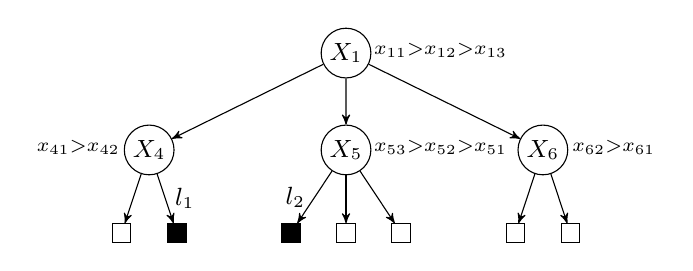
\begin{tikzpicture}[->,>=stealth',
	  level 1/.style={sibling distance=2.5cm, level distance=35pt},
		level 2/.style={sibling distance=0.7cm, level distance=30pt},
		level 3/.style={sibling distance=0.4cm, level distance=30pt}]
	  \node [main node,inner sep=1.5pt,label={[xshift=1.2cm, yshift=-0.5cm]$\scriptstyle x_{11}>x_{12}>x_{13}$}] {$X_1$}
	    child {node [main node,inner sep=1.5pt,label={[xshift=-0.9cm, yshift=-0.5cm]$\scriptstyle x_{41}>x_{42}$}] {$X_4$}
	  		child {node [rectangle,draw] {}}
	  		child {node [rectangle,draw,fill] {} edge from parent node[right] {\small{$l_1$}}}
			}
	    child {node [main node,inner sep=1.5pt,label={[xshift=1.2cm, yshift=-0.5cm]$\scriptstyle x_{53}>x_{52}>x_{51}$}] {$X_5$}
	  		child {node [rectangle,draw,fill] {} edge from parent node[left] {\small{$l_2$}}}
	  		child {node [rectangle,draw] {}}
	  		child {node [rectangle,draw] {}}
	    }
	    child {node [main node,inner sep=1.5pt,label={[xshift=0.9cm, yshift=-0.5cm]$\scriptstyle x_{62}>x_{61}$}] {$X_6$}
	  		child {node [rectangle,draw] {}}
	  		child {node [rectangle,draw] {}}
	    };
	\end{tikzpicture}
  \caption{PLP-tree $T$ over the car domain\label{fig:PLPT_full_ex}}
\end{figure}

Let us consider two cars. 
Car $c_1$ is a white Ford minivan with a capacity of 7 or more, 
a middle-range price, and an automatic transmission; that is,
$c_1=\la x_{11},x_{23}, x_{32}, x_{42}, x_{53}, x_{61} \ra$.
Car $c_2$ is a black Honda sedan with a capacity of 2, a middle-range
price, and a manual transmission:
$c_2=\la x_{12},x_{21}, x_{31}, x_{41}, x_{53}, x_{62} \ra$.
Traversing the tree $T$, we see that $c_1$ reaches leaf $l_1$ of rank $2$
and $c_2$ leaf $l_2$ of rank $3$.
We have $r_T(c_1)<r_T(c_2)$. Thus, we see $c_1 \succ_T c_2$.

\begin{figure}[!ht]
	\centering
  \begin{subfigure}[b]{0.5\textwidth}
		\centering
	  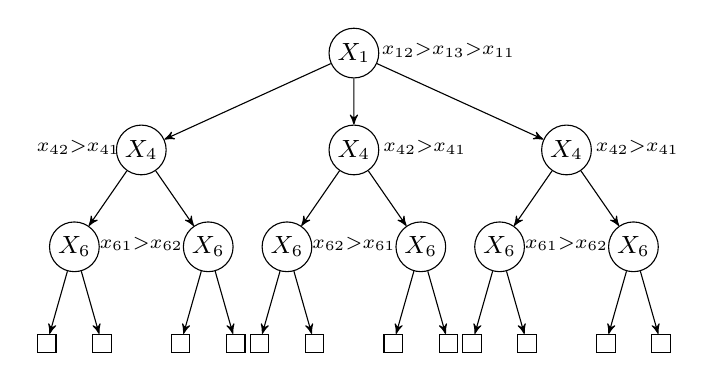
\begin{tikzpicture}[->,>=stealth',
	    level 1/.style={sibling distance=2.7cm, level distance=35pt},
			level 2/.style={sibling distance=1.7cm, level distance=35pt},
			level 3/.style={sibling distance=0.7cm, level distance=35pt}]
	    \node [main node,inner sep=1.5pt,label={[xshift=1.2cm, yshift=-0.5cm]$\scriptstyle x_{12}>x_{13}>x_{11}$}] {$X_1$}
	      child {node [main node,inner sep=1.5pt,label={[xshift=-0.8cm, yshift=-0.5cm]$\scriptstyle x_{42}>x_{41}$}] {$X_4$}
	    		child {node [main node,inner sep=1.5pt] {$X_6$}
	  				child {node [rectangle,draw] {}}
	  				child {node [rectangle,draw] {}}
					}
	    		child {node [main node,inner sep=1.5pt,label={[xshift=-0.85cm, yshift=-0.5cm]$\scriptstyle x_{61}>x_{62}$}] {$X_6$}
	  				child {node [rectangle,draw] {}}
	  				child {node [rectangle,draw] {}}
					}
				}
	      child {node [main node,inner sep=1.5pt,label={[xshift=0.9cm, yshift=-0.5cm]$\scriptstyle x_{42}>x_{41}$}] {$X_4$}
	    		child {node [main node,inner sep=1.5pt] {$X_6$}
	  				child {node [rectangle,draw] {}}
	  				child {node [rectangle,draw] {}}
					}
	    		child {node [main node,inner sep=1.5pt,label={[xshift=-0.85cm, yshift=-0.5cm]$\scriptstyle x_{62}>x_{61}$}] {$X_6$}
	  				child {node [rectangle,draw] {}}
	  				child {node [rectangle,draw] {}}
					}
	      }
	      child {node [main node,inner sep=1.5pt,label={[xshift=0.9cm, yshift=-0.5cm]$\scriptstyle x_{42}>x_{41}$}] {$X_4$}
	    		child {node [main node,inner sep=1.5pt] {$X_6$}
	  				child {node [rectangle,draw] {}}
	  				child {node [rectangle,draw] {}}
					}
	    		child {node [main node,inner sep=1.5pt,label={[xshift=-0.85cm, yshift=-0.5cm]$\scriptstyle x_{61}>x_{62}$}] {$X_6$}
	  				child {node [rectangle,draw] {}}
	  				child {node [rectangle,draw] {}}
					}
	      };
	  \end{tikzpicture}
		\caption{Collapsible PLP-tree \label{fig:UICP_PLPT_full}}
	\end{subfigure}\\
  \begin{subfigure}[b]{0.5\textwidth}
		\centering
	  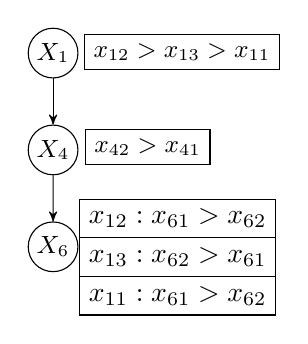
\begin{tikzpicture}[->,>=stealth',
	    level/.style={sibling distance=2.5cm/#1, level distance=35pt}]
	    \node [main node,inner sep=1.5pt] {$X_1$}
	      child {node [main node,inner sep=1.5pt] {$X_4$}
	      	child {node [main node,inner sep=1.5pt] {$X_6$} {}
							child {node [rectangle,draw] at (2.47,3.7) {$x_{12}>x_{13}>x_{11}$} edge from parent[draw=none]}
							child {node [rectangle,draw] at (1.2,2.5) {$x_{42}>x_{41}$} edge from parent[draw=none]}
							child {node [rectangle split, rectangle split parts=3,draw] at (0.75,1.1) 
								{$x_{12}:x_{61}>x_{62}$ \nodepart{second} 
								 $x_{13}:x_{62}>x_{61}$ \nodepart{third}
								 $x_{11}:x_{61}>x_{62}$} edge from parent[draw=none]}
					}
	      };
	  \end{tikzpicture}
		\caption{UICP PLP-tree \label{fig:UICP_PLPT_compact}}
	\end{subfigure}
  \caption{PLP-trees over the car domain}
  \label{fig:UICP}
\end{figure}


\vspace{-0.1cm}
\subsection{Classification of PLP-Trees}

\vspace{-0.1cm}
In the worst case, the size of a PLP-tree is exponential in the number of 
attributes in $\cA$. However, some PLP-trees have a special structure that
allows us to ``collapse'' them and obtain more compact 
representations. This yields a natural classification of PLP-trees, which
we describe below.

%Let $R$ be a sequence of attributes from $\cA$. By $\hat{R}$ we denote the
%set of attributes appearing in $R$. 
Let $R \subseteq \cA$ be the set of attributes that appear in a PLP-tree $T$. We say that $T$ is
\tit{collapsible} if there is a permutation $\hat{R}$ of elements in
$R$ such that for every path in $T$ from the root to a leaf, attributes 
that label nodes on that path appear in the same order in which they 
appear in $\hat{R}$. 

If a PLP-tree $T$ is collapsible, we can represent $T$ by a single path
of nodes labeled with attributes according to the order in which they occur
in $\hat{R}$, 
%(where $\hat{R}$ is the permutation of the set $R$ of attributes in $T$),
where a node labeled with an attribute $X_i$ is also assigned a
\tit{conditional preference table} (CPT) that specifies 
preferences on $X_i$, conditioned on values of ancestor attributes in the path.
These tables make up for the lost structure of $T$ as different ways in 
which ancestor attributes evaluate correspond to different locations 
in the original tree $T$. 
Moreover, missing entries in PCPT of $X_i$ imply equivalence (or 
indifference) between values of $X_i$
under conditions that do not appear in the PCPT.
Clearly, the PLP-tree in \figref{UICP_PLPT_full} is collapsible, and can
be represented compactly as a single-path tree with nodes labeled by 
attributes in the permutation and PCPTs (cf. \figref{UICP_PLPT_compact}).
Note that the PLP-tree in \figref{PLPT_full_ex} is also collapsible and can be collapsed
into a UICP tree.
%Such a collapsed path labeled by attributes is sometimes denoted as
%a sequence of attributes in $\hat{R}$ connected by $\triangleright$, e.g.,
%$X_2\triangleright X_3\triangleright X_1$ for the path in \figref{UICP_PLPT_compact}.

Collapsible PLP-trees represented by a single path of nodes 
will be referred to as \tit{unconditional importance} trees or $\UI$ 
trees, for short. The name reflects the fact that the order in which 
we consider attributes when seeking the rank of an outcome is always the 
same (not conditioned on the values of ancestor attributes of higher importance).

Let $L$ be a collapsible PLP-tree.
If every path in $L$ has the same ordering of attributes
which again is exactly $\hat{R}$, and
for every attribute $X_i$ all nodes in $L$ labeled with $X_i$ have the same
preference on values of $X_i$ (either $1_i>0_i$ or $0_i>1_i$).
Such collapsed 
trees are called $\UI$-$\UP$ PLP-trees, with $\UP$ standing for \tit{unconditional 
preference}. As an example, the $\UI$-$\UP$ tree in \figref{UIUP_PLPT_compact}
is the collapsed representation of the collapsible tree in \figref{UIUP_PLPT_full}.

\begin{figure}[!ht]
	\centering
  \begin{subfigure}[b]{0.23\textwidth}
		\centering
	  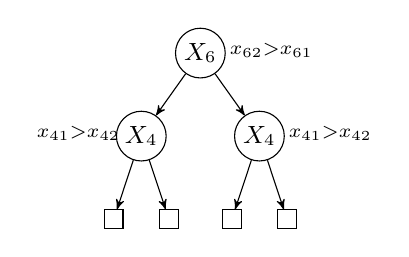
\begin{tikzpicture}[->,>=stealth',
	    level 1/.style={sibling distance=1.5cm, level distance=30pt},
			level 2/.style={sibling distance=0.7cm, level distance=30pt}]
	    \node [main node,inner sep=1.5pt,label={[xshift=0.9cm, yshift=-0.5cm]$\scriptstyle x_{62}>x_{61}$}] {$X_6$}
	      child {node [main node,inner sep=1.5pt,label={[xshift=-0.8cm, yshift=-0.5cm]$\scriptstyle x_{41}>x_{42}$}] {$X_4$}
	    		child {node [rectangle,draw] {}}
	    		child {node [rectangle,draw] {}}
				}
	      child {node [main node,inner sep=1.5pt,label={[xshift=0.9cm, yshift=-0.5cm]$\scriptstyle x_{41}>x_{42}$}] {$X_4$}
	      		child {node [rectangle,draw] {}}
	      		child {node [rectangle,draw] {}}
	      };
	  \end{tikzpicture}
		\caption{Collapsible PLP-tree \label{fig:UIUP_PLPT_full}}
	\end{subfigure}%
  \begin{subfigure}[b]{0.23\textwidth}
		\centering
    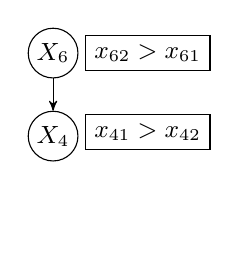
\begin{tikzpicture}[->,>=stealth',node distance=30pt]
      \node[main node,inner sep=1.5pt] (1) {$X_6$};
      \node[rectangle,draw] at (1.2,0) {$x_{62}>x_{61}$};

      \node[main node,inner sep=1.5pt] (2) [below of=1] {$X_4$};
      \node[rectangle,draw] at (1.2,-1) {$x_{41}>x_{42}$};

      \node[rectangle] (3) [below of=2] {};

      \path[]
        (1) edge (2);
    \end{tikzpicture}
		\caption{UIUP PLP-tree \label{fig:UIUP_PLPT_compact}}
	\end{subfigure}\\
  \caption{PLP-trees over the car domain}
  \label{fig:UIUP}
\end{figure}

In all other cases, we refer to collapsed PLP-trees as $\UI$-$\CP$ PLP-trees, 
with $\CP$ standing for \tit{conditional preference}. If preferences on 
an attribute in such a tree depend in an essential way on all preceding 
attributes, there is no real saving in the size of representation (instead 
of an exponential PLP-tree we have a small tree but with preference 
tables that are of exponential size). However, if the preference on an 
attribute depends only on a few higher importance attributes say, never more than 
one or two (or, more generally, never more than some fixed bound $b$), 
the collapsed representation is significantly smaller.

When a PLP-tree is not collapsible, the importance of an attribute depends
on where it is located in the tree. We will refer to such PLP-trees as
\tit{conditional importance} trees or $\CI$ trees.

Let $T$ be a $\CI$ PLP-tree.
We call $T$ a $\CI$-$\UP$ tree if for every attribute $X_i$, 
all nodes in $T$ labeled with $X_i$
have the same preference entry on $X_i$.  
All other non-collapsible PLP-trees are called $\CI$-$\CP$ PLP-trees.
Examples are shown in \figref{CIUP_PLPT} and \figref{CICP_PLPT}.

\begin{figure}[!ht]
	\centering
  \begin{subfigure}[b]{0.25\textwidth}
		\centering
	  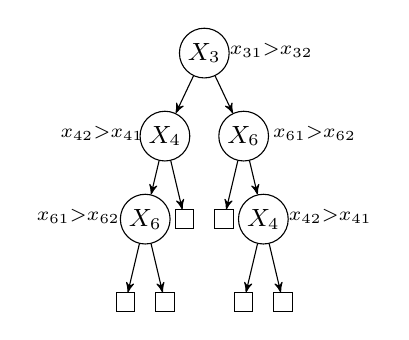
\begin{tikzpicture}[->,>=stealth',
	    level 1/.style={sibling distance=1cm, level distance=30pt},
			level 2/.style={sibling distance=0.5cm, level distance=30pt},
			level 3/.style={sibling distance=0.5cm, level distance=30pt}]
	    \node [main node,inner sep=1.5pt,label={[xshift=0.85cm, yshift=-0.5cm]$\scriptstyle x_{31}>x_{32}$}] {$X_3$}
	      child {node [main node,inner sep=1.5pt,label={[xshift=-0.8cm, yshift=-0.5cm]$\scriptstyle x_{42}>x_{41}$}] {$X_4$}
	    		child {node [main node,inner sep=1.5pt,label={[xshift=-0.85cm, yshift=-0.5cm]$\scriptstyle x_{61}>x_{62}$}] {$X_6$}
	  				child {node [rectangle,draw] {}}
	  				child {node [rectangle,draw] {}}
					}
	  			child {node [rectangle,draw] {}}
				}
	      child {node [main node,inner sep=1.5pt,label={[xshift=0.9cm, yshift=-0.5cm]$\scriptstyle x_{61}>x_{62}$}] {$X_6$}
	  			child {node [rectangle,draw] {}}
	    		child {node [main node,inner sep=1.5pt,label={[xshift=0.85cm, yshift=-0.5cm]$\scriptstyle x_{42}>x_{41}$}] {$X_4$}
	  				child {node [rectangle,draw] {}}
	  				child {node [rectangle,draw] {}}
					}
	      };
	  \end{tikzpicture}
		\caption{CIUP PLP-tree \label{fig:CIUP_PLPT}}
	\end{subfigure}%
  \begin{subfigure}[b]{0.25\textwidth}
		\centering
	  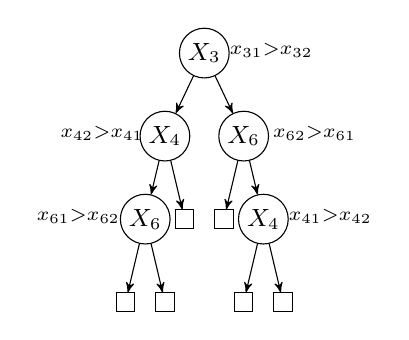
\begin{tikzpicture}[->,>=stealth',
	    level 1/.style={sibling distance=1cm, level distance=30pt},
			level 2/.style={sibling distance=0.5cm, level distance=30pt},
			level 3/.style={sibling distance=0.5cm, level distance=30pt}]
	    \node [main node,inner sep=1.5pt,label={[xshift=0.85cm, yshift=-0.5cm]$\scriptstyle x_{31}>x_{32}$}] {$X_3$}
	      child {node [main node,inner sep=1.5pt,label={[xshift=-0.8cm, yshift=-0.5cm]$\scriptstyle x_{42}>x_{41}$}] {$X_4$}
	    		child {node [main node,inner sep=1.5pt,label={[xshift=-0.85cm, yshift=-0.5cm]$\scriptstyle x_{61}>x_{62}$}] {$X_6$}
	  				child {node [rectangle,draw] {}}
	  				child {node [rectangle,draw] {}}
					}
	  			child {node [rectangle,draw] {}}
				}
	      child {node [main node,inner sep=1.5pt,label={[xshift=0.9cm, yshift=-0.5cm]$\scriptstyle x_{62}>x_{61}$}] {$X_6$}
	  			child {node [rectangle,draw] {}}
	    		child {node [main node,inner sep=1.5pt,label={[xshift=0.85cm, yshift=-0.5cm]$\scriptstyle x_{41}>x_{42}$}] {$X_4$}
	  				child {node [rectangle,draw] {}}
	  				child {node [rectangle,draw] {}}
					}
	      };
	  \end{tikzpicture}
		\caption{CICP PLP-tree \label{fig:CICP_PLPT}}
	\end{subfigure}
  \caption{CI PLP-trees over the car domain}
  \label{fig:CI}
\end{figure}


\section{Partial Lexicographic Preference Forests}
We introduce a new notion of
\tit{PLP-forests} that is a collection of PLP-trees.
Let $F$ be a PLP-forest such that $F = \{T_1,\ldots,T_n\}$.
Let us denote by $N_F(o_1,o_2)=|\{T \in F:o_1 \succ_T o_2\}|$
the number of trees in the forests where the outcome $o_1$ is
preferred to the outcome $o_2$.
Now consider the dominance testing problem.
Given a preference forest $F$, and two outcomes $o_1$ and $o_2$,
we say that $o_1 \succ_F^\Maj o_2$ iff $N_F(o_1,o_2)>N_F(o_2,o_1)$,
and that $o_1 \approx_F^\Maj o_2$ iff $N_F(o_1,o_2)=N_F(o_2,o_1)$,
where $\Maj$ stands for the majority rule.
Indeed, the majority rule is an intuitive and computationally easy
preference aggregation rule.
In general, the majority rule may lead to the so-called Condorcet paradox, where
the $\succ_F^\Maj$ relation contains a cycle.
However, it is not the case for our datasets.
Other possible aggregators are positional
scoring rules (adjusted for total \tit{preorders}), Copeland's
method, among others.


\section{Problems and Complexities}
In this work, we focus on the \tsc{MaxLearn} problem as follows for PLP-trees.
\begin{definition}
	Maximal-learning (\tsc{MaxLearn}): given an example set $\cE$ and a 
	positive integer $k$ ($k \leq |\cE|$), decide whether there exists a PLP-tree 
	$T$ (of a particular type) such that $T$ satisfies at least $k$ examples 
	in $\cE$.
\end{definition}

The \tsc{MaxLearn} problem has been shown NP-complete
for all four classes of PLP-trees\cite{conf/aaai15/LiuT}.
The following problems are also of interest.

\begin{definition}
	Best-linearization (\tsc{BestLin}): Given a directed graph $G=(V,E)$,
	find the best linearization, that is, the total order 
	$\succ$ over $V$ that agrees with the as many 
	edges $uv \in E$ as possible.
\end{definition}
This problem is related to solving the MaxLearn problem,
when we need to pick a preference entry for an attribute,
although it is trivial as we bound the sizes of the
attribute domains by a constant.
We now show the complexity of the \tsc{BestLin} problem,
if it has not been proved yet.

\begin{thm}
	The \tsc{BestLin} problem is NP-hard.
\end{thm}
\begin{proof}
	To show NP-hardness, it suffices to show that the \tsc{BestLin}
	is at least as hard as another NP-hard problem:
	the Minimum Feedback Arc Set (MFAS) problem\footnote{
		Given a directed graph $G=(V,E)$, 
		the Minimum Feedback Arc Set (MFAS) problem 
		is to find the subset
		$F \subseteq E$ such that $G'=(V,E\backslash F)$
		is acyclic and $|F|$ is minimum.
	}.
	To solve the \tsc{BestLin} problem, we can first
	solve the MFAS problem and then apply the topological
	sorting, taking linear time, on the solution to obtain
	the best linearization.
\end{proof}

Schmitt and Martegnon\cite{schmitt2006complexity} proved that, 
for UIFP trees\footnote{
	UIFP is subclass of UIUP trees where preference entries for all
	attributes are fixed.
}, the greedy heuristic approximates the \tsc{MaxLearn} problem
to within a factor of $p$.
We are interested in extending this results to more general classes
of trees.
Yet another problem we might want to study is the \tsc{MaxLearn} problem
in the setting of PLP-forests.
That is, given an example set $\cE$ and positive integers $f$ and $k$,
decide whether there exists a PLP-forest $F$ of size $f$ that satisfies
at least $k$ examples in $\cE$.


\section{Preference Learning Library}
Here we describe how we built the datasets\footnotemark to 
support preference learning experiments.
We limited the number of issues to 10, and the size of
their domains to 4 if it is more than 4.
The description of the datasets in this library are shown
in \tblref{description}, where we denote by $p$ the number
of attributes, $|\cX|$ the number of outcomes,
$|\cE^\succ|$ the number of strict examples, and
$|\cE^\approx|$ the number of equivalent examples.

\footnotetext{We will make the library public once the paper is accepted.}

\smallskip \noindent \textbf{BreastCancerWisconsin \ }
The BreastCancerWisconsin dataset has 270 outcomes over 9 attributes.
To generate equivalent and strict examples for the dataset,
we assume that outcomes labeled by ``benign" are better than
those by ``malignant."
For equivalent examples, we have that outcomes labeled by ``benign" are equivalent
to one another, so are those labeled by ``malignant."

\smallskip \noindent \textbf{CarEvaluation \ }
The CarEvaluation dataset has 1728 outcomes over 6 attributes.
To generate equivalent and strict examples for the dataset,
we assume that outcomes labeled by ``vgood" are better than
those by ``good," which are better than those
by ``acc," which are preferred to those by ``unacc."

\smallskip \noindent \textbf{CreditApproval \ }
The CreditApproval dataset has 520 outcomes over 10 attributes.
To generate equivalent and strict examples for the dataset,
we assume that outcomes labeled by ``+" (positive) are better than
those by ``-" (negative).

\smallskip \noindent \textbf{GermanCredit \ }
The GermanCredit dataset has 914 outcomes over 10 attributes.
To generate equivalent and strict examples for the dataset,
we assume that outcomes labeled by ``1" (good) are better than
those by ``2" (bad).

\smallskip \noindent \textbf{Ionosphere \ }
The Ionosphere dataset has 118 outcomes over 10 attributes.
To generate equivalent and strict examples for the dataset,
we assume that outcomes labeled by ``g" (good) are better than
those by ``b" (bad).

\smallskip \noindent \textbf{MammographicMass \ }
The MammographicMass dataset has 118 outcomes over 10 attributes.
To generate equivalent and strict examples for the dataset,
we assume that outcomes labeled by ``0" (benign) are better than
those by ``1" (malignant).

\smallskip \noindent \textbf{Mushroom \ }
The Mushroom dataset has 184 outcomes over 10 attributes.
To generate equivalent and strict examples for the dataset,
we assume that outcomes labeled by ``e" (edible) are better than
those by ``p" (poisonous).

\smallskip \noindent \textbf{Nursery \ }
The Nursery dataset has 184 outcomes over 10 attributes.
To generate equivalent and strict examples for the dataset,
we assume that outcomes labeled by ``spec\_prior" are better than
those by ``priority," which are better than those
by ``very\_recom," which are preferred to those by ``recommend,"
which again are better than those by ``not\_recom."

\smallskip \noindent \textbf{SPECTHeart \ }
The SPECTHeart dataset has 115 outcomes over 10 attributes.
To generate equivalent and strict examples for the dataset,
we assume that outcomes labeled by ``0" (positive) are better than
those by ``1" (negative).

\smallskip \noindent \textbf{TicTacToe \ }
The TicTacToe dataset has 958 outcomes over 9 attributes.
To generate equivalent and strict examples for the dataset,
we assume that outcomes labeled by ``positive" are better than
those by ``negative".

\smallskip \noindent \textbf{Vehicle \ }
The Vehicle dataset has 455 outcomes over 10 attributes.
To generate equivalent and strict examples for the dataset,
we assume that outcomes labeled by ``bus" are better than
those by ``opel," which are better than those
by ``saab," which are preferred to those by ``van."

\smallskip \noindent \textbf{Wine \ }
The Wine dataset has 455 outcomes over 10 attributes.
To generate equivalent and strict examples for the dataset,
we assume that outcomes labeled by ``1" are better than
those by ``2," which are better than those
by ``3."


\begin{table}
	\centering
	\small
	\begin{tabular}{ |c||c|c|c|c| } 
		\hline
		Dataset                 & $p$  & $|\cX|$ & $|\cE^\succ|$ & $|\cE^\approx|$ \\
		\hline \hline
		BreastCancerWisconsin   & 9 & 270 & 9,009 & 27,306 \\ 
		\hline
		CarEvaluation           & 6 & 1728 & 682,721 & 809,407\\ 
		\hline
		CreditApproval          & 10 & 520 & 66,079 & 68,861 \\
		\hline
		GermanCredit            & 10 & 914 & 172,368 & 244,873 \\
		\hline
		Ionosphere              & 10 & 118 & 3,472 & 3,431 \\
		\hline
		MammographicMass        & 5 & 62 & 792 & 1,099 \\
		\hline
		Mushroom                & 10 & 184 & 8,448 & 8,388 \\
		\hline
		Nursery                 & 8 & 1,266 & 548,064 & 252,681 \\
		\hline
		SPECTHeart              & 10 & 115 & 3,196 & 3,359 \\
		\hline
		TicTacToe               & 9 & 958 & 207,832 & 250,571 \\
		\hline
		Vehicle                 & 10 & 455 & 76,713 & 26,572 \\
		\hline
		Wine                    & 10 & 177 & 10,322 & 5,254 \\
		\hline
	\end{tabular}
	\caption{Description of datasets in the library}
	\label{tbl:description}
\end{table}



\section{Experimentation}
We design and implement exact and approximating systems to evaluate PLP-trees and forests of
PLP-trees.

\subsection{Evaluating PLP-Trees}
To evaluate the feasibility of PLP-trees of various classes,
we implemented an exact learner using Answer-Set Programming,
as well as a greedy learning algorithm.

First, for all datasets we achieve results for UIUP PLP-trees
using exact and greedy learning methods, and for decision trees.
For dataset $D$, we randomly pick $\R_D \subset \strictEx$ with $1 \leq |\R_D| \leq 250$
as the set of \tit{training} examples,
and $\T_D = \strictEx \setminus \R_D$ as the set of \tit{testing} examples.
Then, from $\R_D$, we train a UIUP PLP-tree $T_X$ using Answer-Set Programming 
such that $T_X$ decides the most examples in $\R_D$, and another UIUP PLP-tree $T_\MH$ using
greedy heuristic.
To compare our preference trees with decision trees, we also train a decision tree $T_\DT$
from $\R_D$.
Finally, on $\T_D$ we test the models $T_X$, $T_\MH$ and $T_\DT$ to compute the percentages of 
strict examples in $\T_D$ that are correctly decided by them.
This process is repeated $20$ times for all the datasets, and the average results are reported
as \tit{learning curves} presented in \figref{B1}, \figref{Car1}, \figref{Crd1}, 
\figref{G1}, \figref{I1}, \figref{Mam1}, \figref{Mush1}, \figref{N1}, \figref{S1}, 
\figref{T1}, \figref{V1}, and \figref{W1}.

What we have learned from \figref{trees1}:
\begin{enumerate}
	\item For the exact learning method using ASP (X-UIUP),
				learned UIUP trees achieve over 70\% of accuracy across all datasets using small 
				samples of 250 examples:
				70\%-80\%: 3 datasets, 80\%-90\%: 5 datasets, and 90\%-100\%: 4 datasets.
	\item For the greedy heuristic method (MH-UIUP),
				t learned UIUP trees achieve also over 70\% of accuracy across all datasets using small
				samples of 250 examples:
				70\%-80\%: 5 datasets, 80\%-90\%: 4 datasets, and 90\%-100\%: 3 datasets.
	\item For the exact search method used in \tit{fitctree}, a matlab tool for classification decision tree (DT),
				learned decision trees achieve over 60\% of accuracy across all datasets using small 
				samples of 250 examples: 60\%-70\%:  2 datasets,
				70\%-80\%: 1 datasets, 80\%-90\%: 6 datasets, and 90\%-100\%: 3 datasets.
	\item Comparing X-UIUP and DT, we observe that X-UIUP outperforms DT on 8 datasets (
				CreditApproval, GermanCredit, Ionosphere, Nursery, SpectHeart, TicTacToe, Vehicle,
				and Wine), that DT outperforms X-UIUP on 2 datasets (CarEvaluation and Mushroom),
				that X-UIUP and DT are close on the other 2 datasets (BreastCancerWisconsin and
				MammographicMass). 
				Comparing M-UIUP and DT, we observe that MH-UIUP outperforms DT on 7 datasets (
				CreditApproval, GermanCredit, Nursery, SpectHeart, TicTacToe, Vehicle,
				and Wine), that DT outperforms MH-UIUP on 2 datasets (CarEvaluation and Mushroom),
				that MH-UIUP and DT are close on the other 3 datasets (BreastCancerWisconsin, Ionosphere, and
				MammographicMass).
				This comparison shows UIUP trees, the simplest PLP-trees, are favored over decision trees
				in terms of both accuracy and representation intuition, when training samples are of
				small sizes.
	\item Comparing X-UIUP and MH-UIUP, we see that mostly the greedy heuristic is close to
				the exact algorithm, except for 2 datasets: Ionosphere and Mushroom.
				This indicates the greedy method works well.
\end{enumerate}



\begin{figure*}[ht]
	\centering

  \begin{subfigure}[b]{0.3\textwidth}
		\centering
		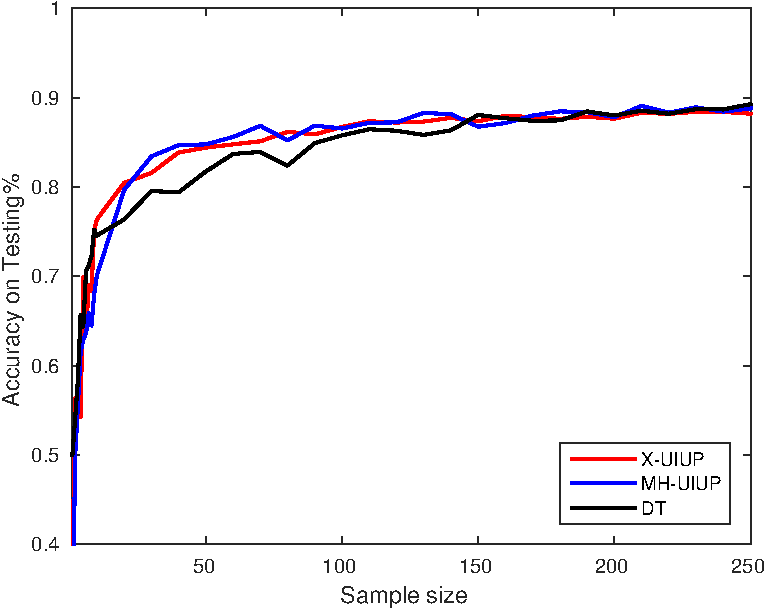
\includegraphics[width=\textwidth]{figs/PLPTF/Trees/BreastCancerWisconsinDownsampled_Trees_X_MH.pdf}
		\caption{BreastCancerWisconsin}
		\label{fig:B1}
	\end{subfigure}
  \begin{subfigure}[b]{0.3\textwidth}
		\centering
  	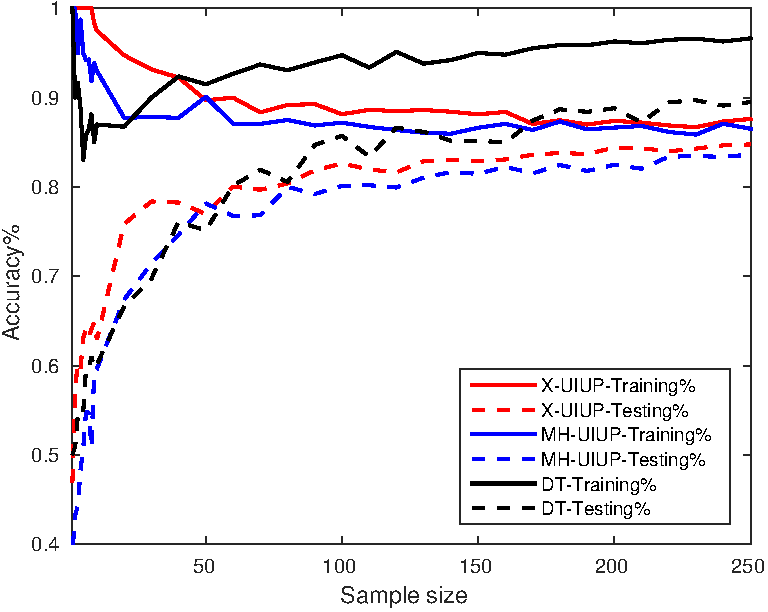
\includegraphics[width=\textwidth]{figs/PLPTF/Trees/CarEvaluation_Trees_X_MH.pdf}
  	\caption{CarEvaluation}
		\label{fig:Car1}
	\end{subfigure}
  \begin{subfigure}[b]{0.3\textwidth}
		\centering
  	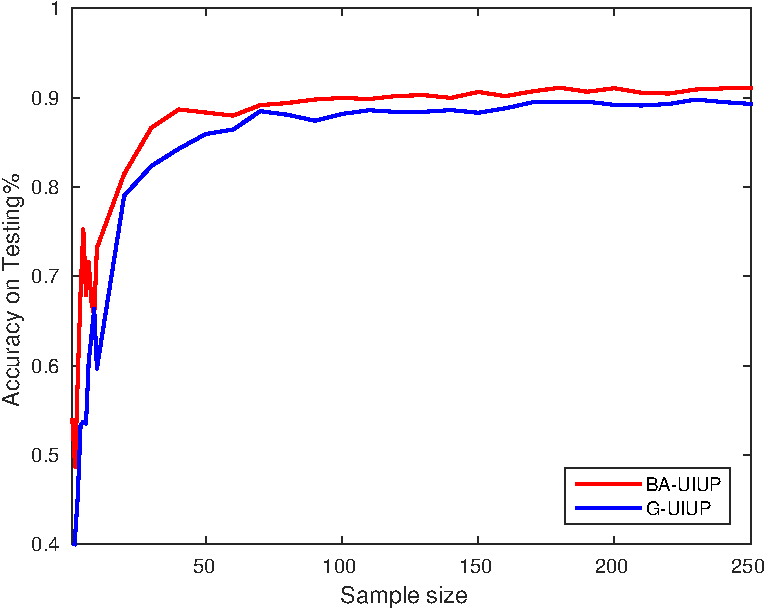
\includegraphics[width=\textwidth]{figs/PLPTF/Trees/CreditApprovalDownsampledFurther_Trees_X_MH.pdf}
  	\caption{CreditApproval}
		\label{fig:Crd1}
	\end{subfigure}
  \\
  \begin{subfigure}[b]{0.3\textwidth}
		\centering
  	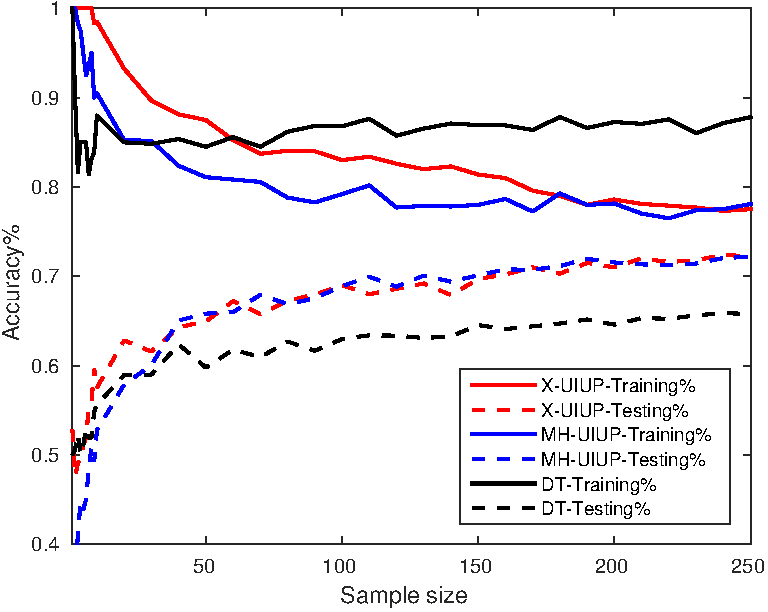
\includegraphics[width=\textwidth]{figs/PLPTF/Trees/GermanCreditDownsampledFurther_Trees_X_MH.pdf}
  	\caption{GermanCredit}
		\label{fig:G1}
	\end{subfigure}
  \begin{subfigure}[b]{0.3\textwidth}
		\centering
  	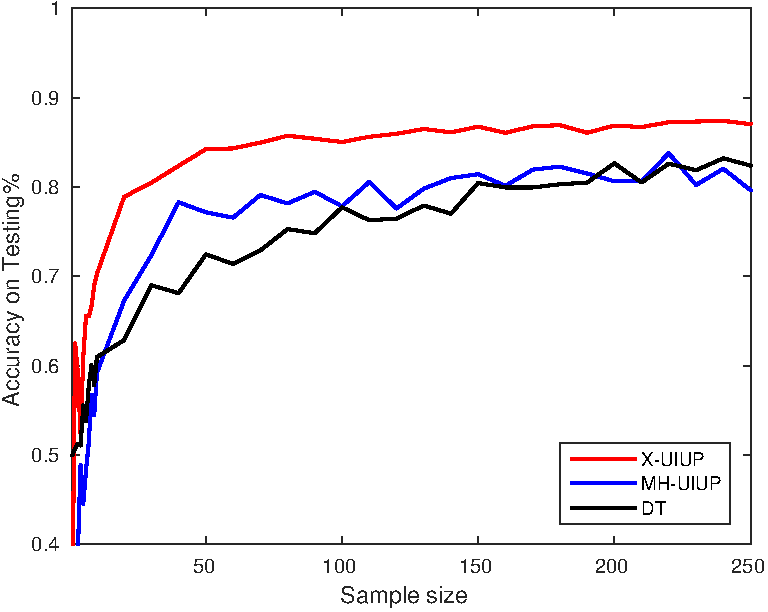
\includegraphics[width=\textwidth]{figs/PLPTF/Trees/IonosphereDownsampledFurther_Trees_X_MH.pdf}
  	\caption{Ionosphere}
		\label{fig:I1}
	\end{subfigure}
  \begin{subfigure}[b]{0.3\textwidth}
		\centering
  	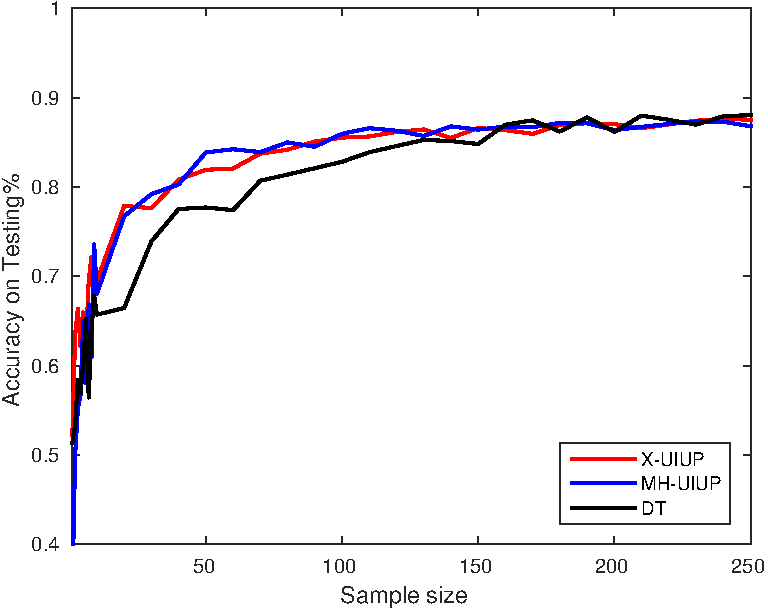
\includegraphics[width=\textwidth]{figs/PLPTF/Trees/MammographicMassDownsampled_Trees_X_MH.pdf}
  	\caption{MammographicMass}
		\label{fig:Mam1}
	\end{subfigure}
	\\
  \begin{subfigure}[b]{0.3\textwidth}
		\centering
  	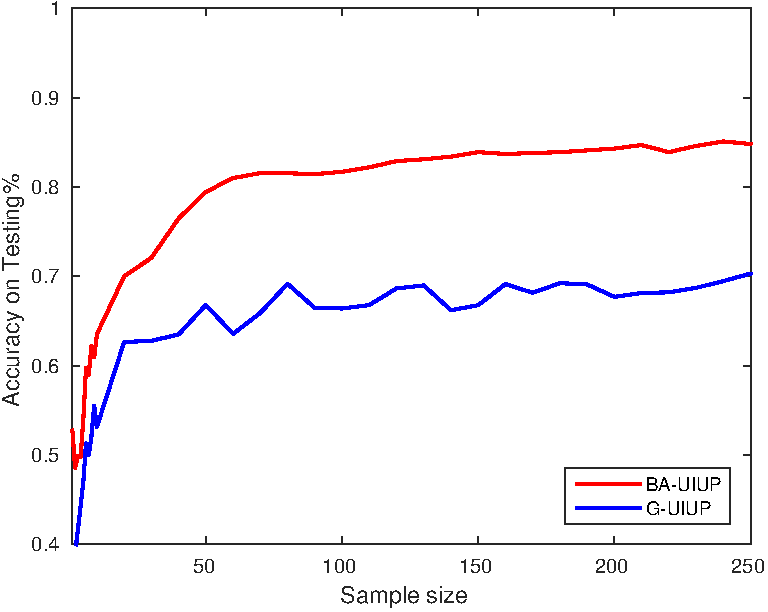
\includegraphics[width=\textwidth]{figs/PLPTF/Trees/MushroomDownsampled_Trees_X_MH.pdf}
  	\caption{Mushroom}
		\label{fig:Mush1}
	\end{subfigure}
  \begin{subfigure}[b]{0.3\textwidth}
		\centering
  	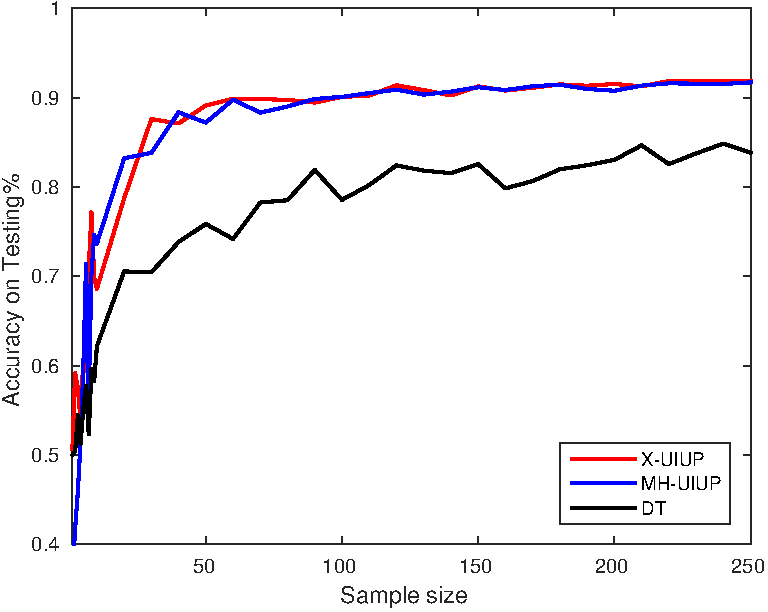
\includegraphics[width=\textwidth]{figs/PLPTF/Trees/NurseryDownsampledFurther_Trees_X_MH.pdf}
  	\caption{Nursery}
		\label{fig:N1}
	\end{subfigure}
  \begin{subfigure}[b]{0.3\textwidth}
		\centering
  	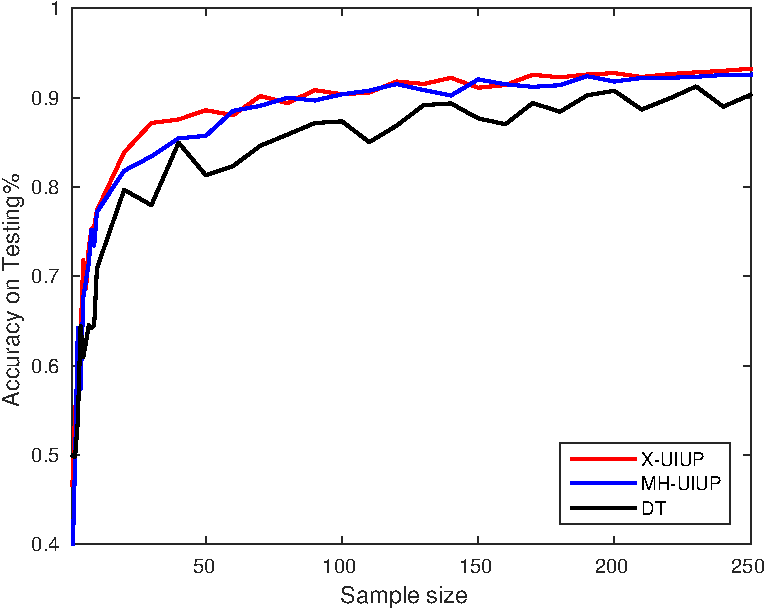
\includegraphics[width=\textwidth]{figs/PLPTF/Trees/SpectHeartDownsampledFurther_Trees_X_MH.pdf}
  	\caption{SpectHeart}
		\label{fig:S1}
	\end{subfigure}
  \\
  \begin{subfigure}[b]{0.3\textwidth}
		\centering
  	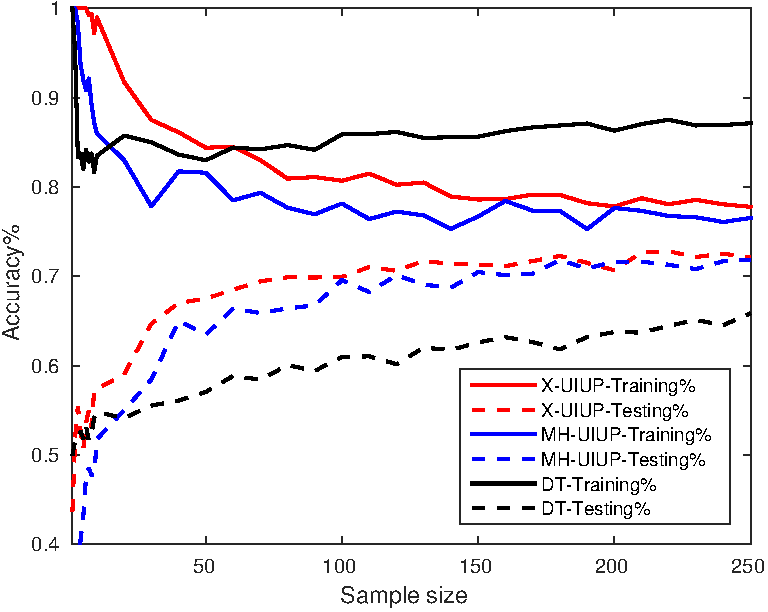
\includegraphics[width=\textwidth]{figs/PLPTF/Trees/TicTacToe_Trees_X_MH.pdf}
  	\caption{TicTacToe}
		\label{fig:T1}
	\end{subfigure}
  \begin{subfigure}[b]{0.3\textwidth}
		\centering
  	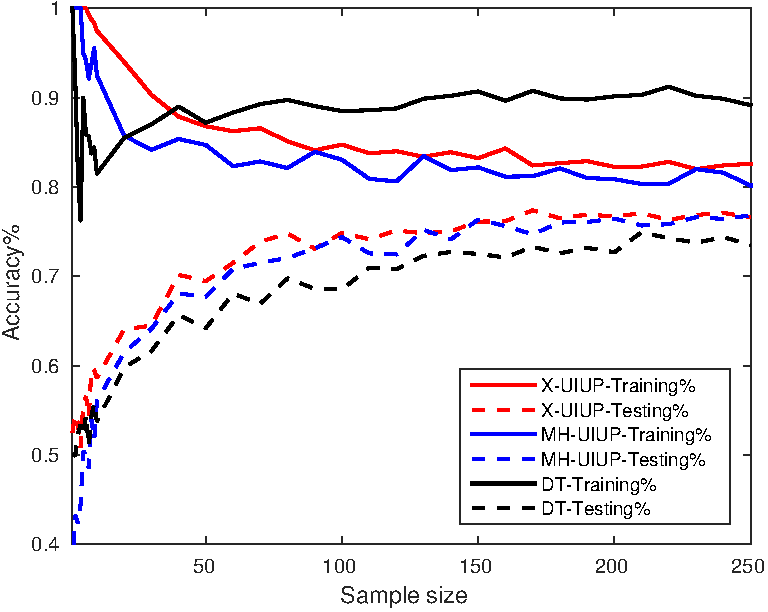
\includegraphics[width=\textwidth]{figs/PLPTF/Trees/VehicleDownsampledFurther_Trees_X_MH.pdf}
  	\caption{Vehicle}
		\label{fig:V1}
	\end{subfigure}
  \begin{subfigure}[b]{0.3\textwidth}
		\centering
  	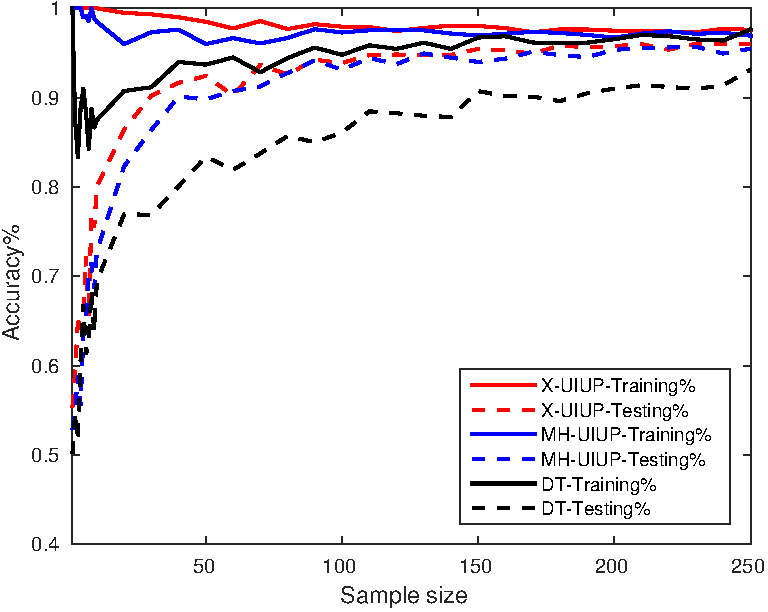
\includegraphics[width=\textwidth]{figs/PLPTF/Trees/WineDownsampled_Trees_X_MH.pdf}
  	\caption{Wine}
		\label{fig:W1}
	\end{subfigure}

  \caption{UIUP PLP-trees vs. decision trees}
  \label{fig:trees1}
\end{figure*}

Next, since X-UIUP does not scale well even for small samples of sizes near
250, we have performed experiments with more expansive samples using the greedy
heuristic on all four classes of PLP-trees: UIUP, UICP-1, CIUP and CICP.
For dataset $\cE^\succ$, we generate $R_{\cE^\succ}$ 
($1\%*|\cE^\succ| \leq |\R_{\cE^\succ}| \leq 70\%*|\cE^\succ|$)
and $\T_{\cE^\succ}$ ($\T_{\cE^\succ}=\cE^\succ \backslash \R_{\cE^\succ}$) 
for training and testing, respectively.
Then, from $\R_{\cE^\succ}$, we train UIUP, UICP-1, CIUP and CICP trees
($T_1$, $T_2$, $T_3$ and $T_4$) using the greedy heuristic.
Finally, on $\T_{\cE^\succ}$ we test the models $T_1$, $T_2$, $T_3$ and $T_4$ to compute the percentages of 
strict examples in $\T_{\cE^\succ}$ that are correctly decided by them.
In \tblref{trees2}, we present results of accuracy on testing using 70\% of $\cE^\succ$
in the training phase.

\begin{table}
  \centering
  \small
  \begin{tabular}{ |c||c|c|c|c| }
    \hline
    Dataset          				& UIUP & UICP-1 & CIUP & CICP \\
    \hline \hline
    BreastCancerWisconsin   & 90.7 & 91.4 & 90.7 & 91.4 \\
    \hline                                            
    CarEvaluation           & 85.8 & 86.0 & 85.9 & 86.0 \\
    \hline                                            
    CreditApproval          & 91.4 & 91.7 & 92.0 & 92.2 \\
    \hline                                            
    GermanCredit            & 74.3 & 74.6 & 74.5 & 75.7 \\
    \hline                                            
    Ionosphere              & 87.1 & [86.9] & 88.5 & 90.4 \\
    \hline                                            
    MammographicMass        & 88.2 & 89.5 & [86.9] & 90.0 \\
    \hline                                            
    Mushroom                & 71.6 & 74.2 & 75.6 & 76.6 \\
    \hline                                            
    Nursery                 & 92.9 & 93.0 & 93.0 & 93.0 \\
    \hline                                            
    SPECTHeart              & 93.4 & 94.9 & 94.8 & 95.7 \\
    \hline                                            
    TicTacToe               & 73.9 & 74.5 & 75.4 & 76.2 \\
    \hline                                            
    Vehicle                 & 79.2 & 80.4 & 80.0 & 81.2 \\
    \hline                                            
    Wine                    & 95.5 & 97.8 & 97.5 & 97.8 \\
    \hline
  \end{tabular}
  \caption{Accuracy percents on the testing data (30\% of $\cE^\succ$)
					 for all four classes of PLP-trees, using models learned
					 by the greedy algorithm from the learning 
					 data (the other 70\% of $\cE^\succ$)}
  \label{tbl:trees2}
\end{table}

What we have learned from \tblref{trees2}:
\begin{enumerate}
	\item UIUP trees performs well, with all datasets above 70\%, and
				4 datasets (GermanCredit,
				Mushroom, TicTacToe and Vehicle) below 85\%.
	\item UICP-1 trees outperforms UIUP trees on all but one dataset
				Ionosphere.
	\item CIUP trees outperforms UIUP trees on all but one dataset
				MammographicMass.
	\item CICP trees outperforms all other classes of trees on all
				datasets.
\end{enumerate}


\subsection{Evaluating PLP-Forests}
To further boost up performances, we now show empirical results
of learning \tit{PLP-forests}.

First, we show results for UIUP PLP-forests using exact learning
and the greedy heuristic.
In each experiment, we randomly partition a dataset into training
set (70\%) and testing set (30\%), learn a forest (the size of it
indicated by on the x-axis) where
each tree is learned from 50 randomly selected examples from the
training set, and test the forest against the testing set.
We repeat it 20 times and report the average accuracy (indicated on
the y-axis) in the plots.
Note that the plots also include a straight line representing
the result for learning a UIUP PLP-tree, had we used all the
training data to learn a single tree using the greedy heuristic.

\begin{table}
  \centering
  \small
  \begin{tabular}{ |c||c|c|c| }
    \hline
    Dataset          				& MH+Tree & MH+Forest & X+Forest\\
    \hline \hline
    BreastCancerWisconsin   & 90.7 & 93.4 & 95.1 \\
    \hline                                     
    CarEvaluation           & 85.8 & 91.9 & [89.2] \\
    \hline                                     
    CreditApproval          & 91.4 & 91.5 & 93.1 \\
    \hline                                     
    GermanCredit            & 74.3 & 75.4 & 77.9 \\
    \hline                                     
    Ionosphere              & 87.1 & [83.0] & 92.5 \\
    \hline                                     
    MammographicMass        & 88.2 & 89.1 & 90.8 \\
    \hline                                     
    Mushroom                & 71.6 & 78.8 & 90.2 \\
    \hline                                     
    Nursery                 & 92.9 & 93.2 & 94.0 \\
    \hline                                     
    SPECTHeart              & 93.4 & 93.7 & 94.9 \\
    \hline                                     
    TicTacToe               & 73.9 & 75.1 & 77.2 \\
    \hline                                     
    Vehicle                 & 79.2 & 82.7 & [81.9] \\
    \hline                                     
    Wine                    & 95.5 & 95.8 & 96.9 \\
    \hline
  \end{tabular}
  \caption{Accuracy percents on the testing data (30\% of $\cE^\succ$)
					 for UIUP trees and forests of 5000 UIUP trees, 
					 using the greedy and exact algorithms from the learning 
					 data (the other 70\% of $\cE^\succ$)}
  \label{tbl:forests1}
\end{table}

What we have learned from \tblref{forests1}:
\begin{enumerate}
	\item UIUP forests using the greedy method
				outperforms UIUP trees using the greedy method on all
				but one dataset: Ionosphere.
				Average improvement is 1.63\%.
	\item UIUP forests using the exact algorithm
				outperforms UIUP trees using the greedy method on all
				datasets.
				Average improvement is 4.14\%.
	\item UIUP forests using the exact algorithm
				outperforms UIUP forests using the greedy method on all
				but two datasets: CarEvaluation and Vehicle.
				Average improvement is 2.51\%.
\end{enumerate}


Second, we show results for UIUP PLP-forests using the greedy
heuristic with different learning sample size per tree.
The setting is similar to the previous one.
These results are shown in \figref{B4}, \figref{Car4}, \figref{Crd4}, \figref{I4},
\figref{Mam4}, \figref{S4}, \figref{T4}, \figref{V4}, and \figref{W4}.

\begin{figure*}[ht]
	\centering

  \begin{subfigure}[b]{0.3\textwidth}
		\centering
		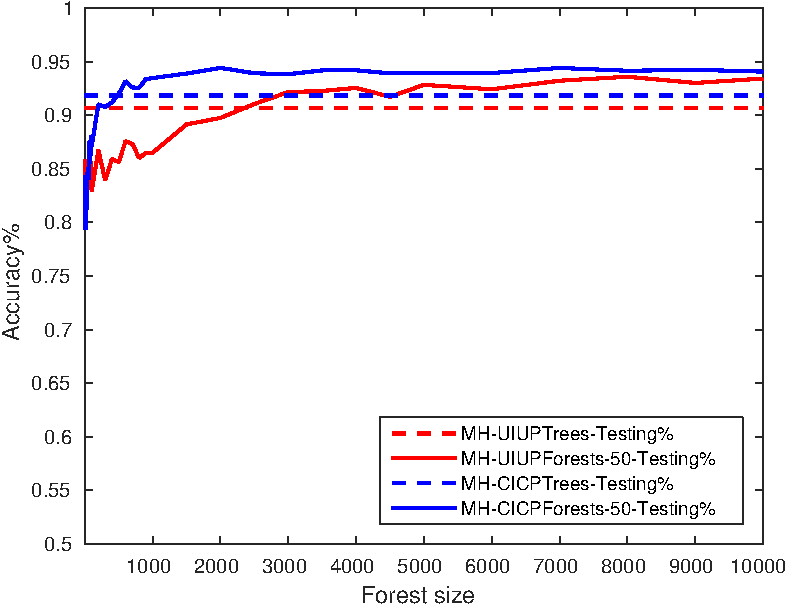
\includegraphics[width=\textwidth]{figs/PLPTF/Forests/BreastCancerWisconsinDownsampled_Forests_MH.pdf}
		\caption{BreastCancerWisconsin}
		\label{fig:B4}
	\end{subfigure}
  \begin{subfigure}[b]{0.3\textwidth}
		\centering
  	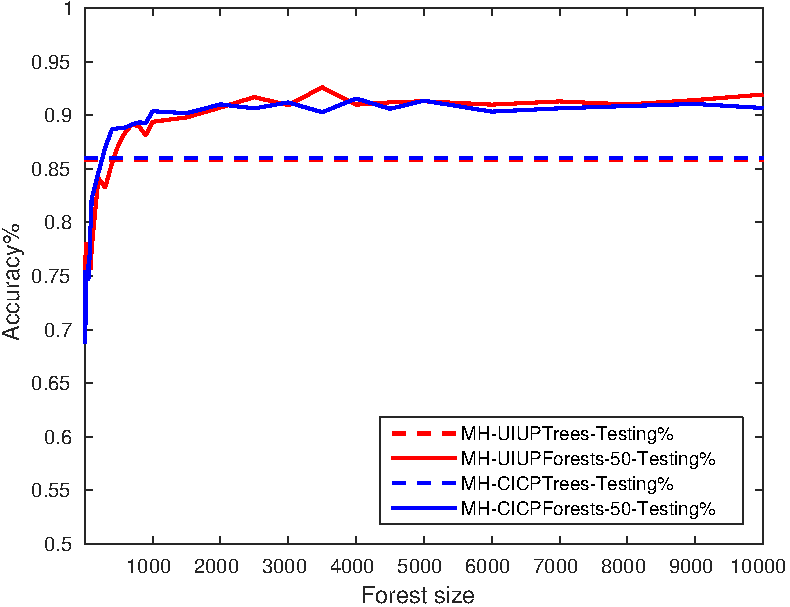
\includegraphics[width=\textwidth]{figs/PLPTF/Forests/CarEvaluation_Forests_MH.pdf}
  	\caption{CarEvaluation}
		\label{fig:Car4}
	\end{subfigure}
  \begin{subfigure}[b]{0.3\textwidth}
		\centering
  	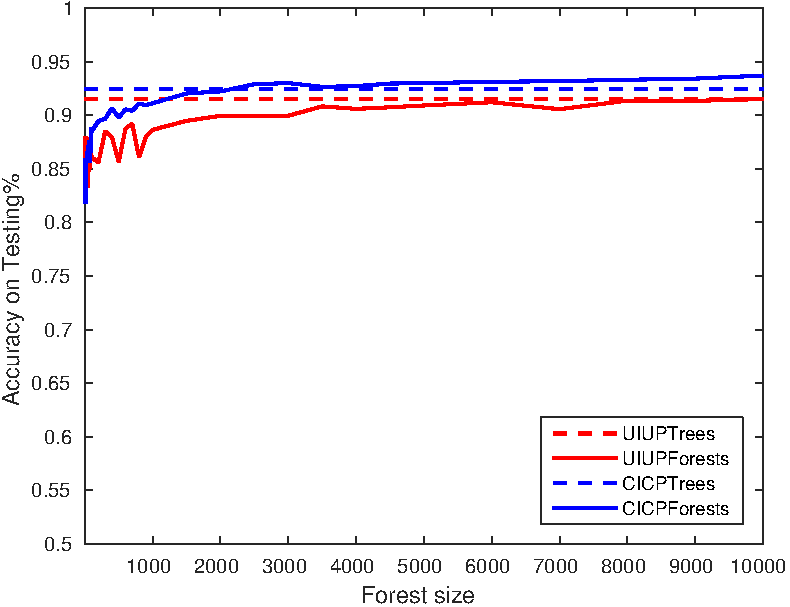
\includegraphics[width=\textwidth]{figs/PLPTF/Forests/CreditApprovalDownsampledFurther_Forests_MH.pdf}
  	\caption{CreditApproval}
		\label{fig:Crd4}
	\end{subfigure}
  \\
  \begin{subfigure}[b]{0.3\textwidth}
		\centering
  	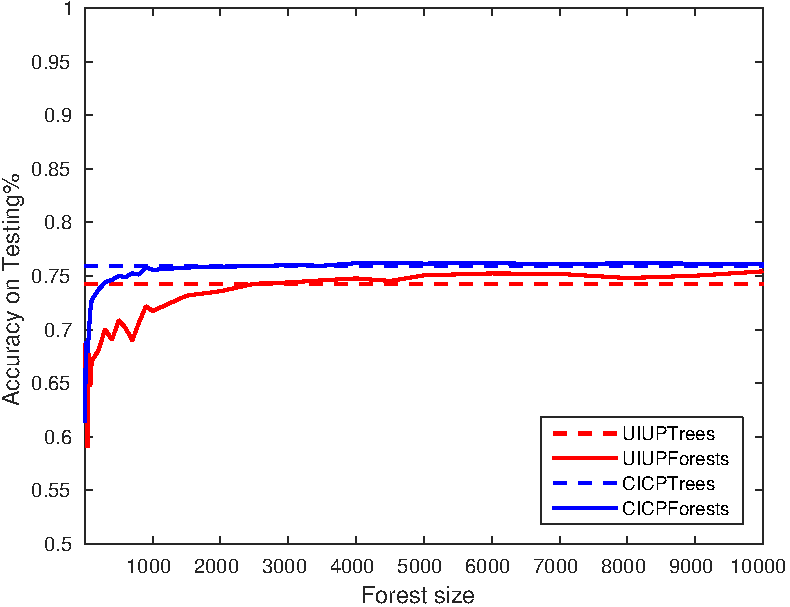
\includegraphics[width=\textwidth]{figs/PLPTF/Forests/GermanCreditDownsampledFurther_Forests_MH.pdf}
  	\caption{GermanCredit}
		\label{fig:G4}
	\end{subfigure}
  \begin{subfigure}[b]{0.3\textwidth}
		\centering
  	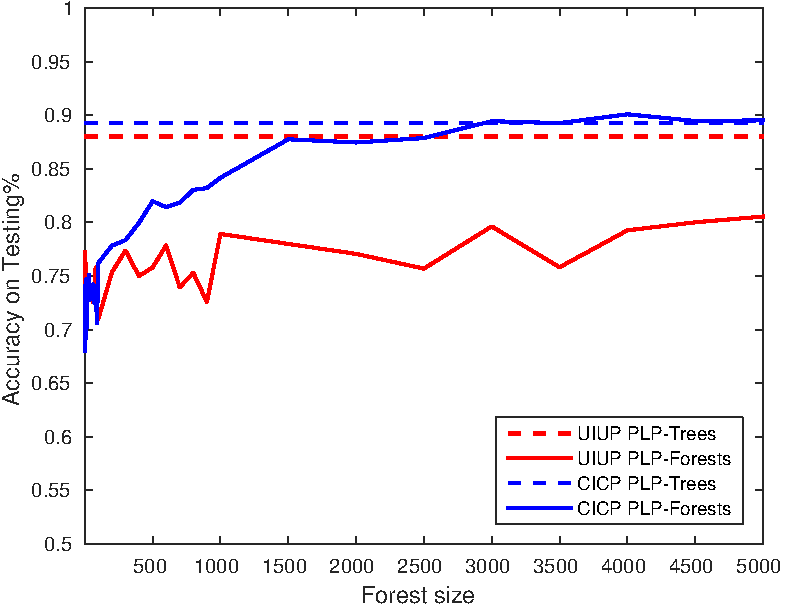
\includegraphics[width=\textwidth]{figs/PLPTF/Forests/IonosphereDownsampledFurther_Forests_MH.pdf}
  	\caption{Ionosphere}
		\label{fig:I4}
	\end{subfigure}
  \begin{subfigure}[b]{0.3\textwidth}
		\centering
  	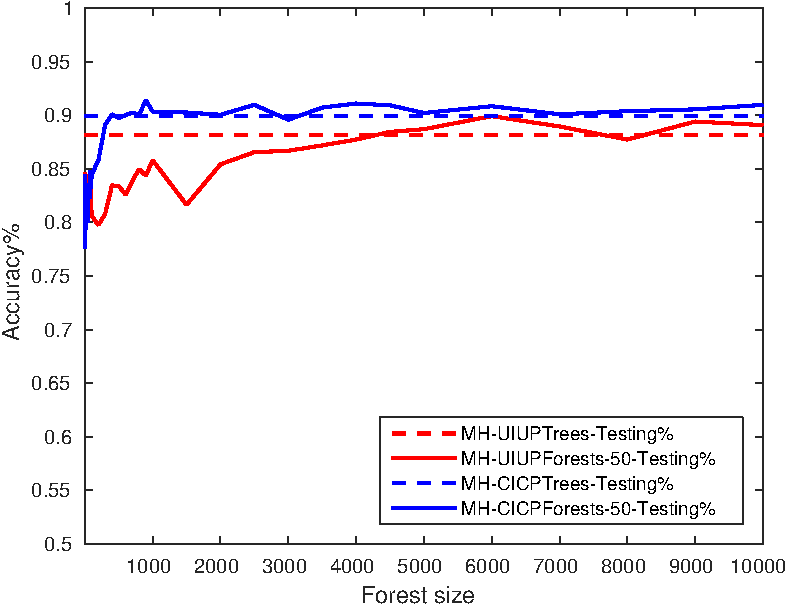
\includegraphics[width=\textwidth]{figs/PLPTF/Forests/MammographicMassDownsampled_Forests_MH.pdf}
  	\caption{MammographicMass}
		\label{fig:Mam4}
	\end{subfigure}
	\\
  \begin{subfigure}[b]{0.3\textwidth}
		\centering
  	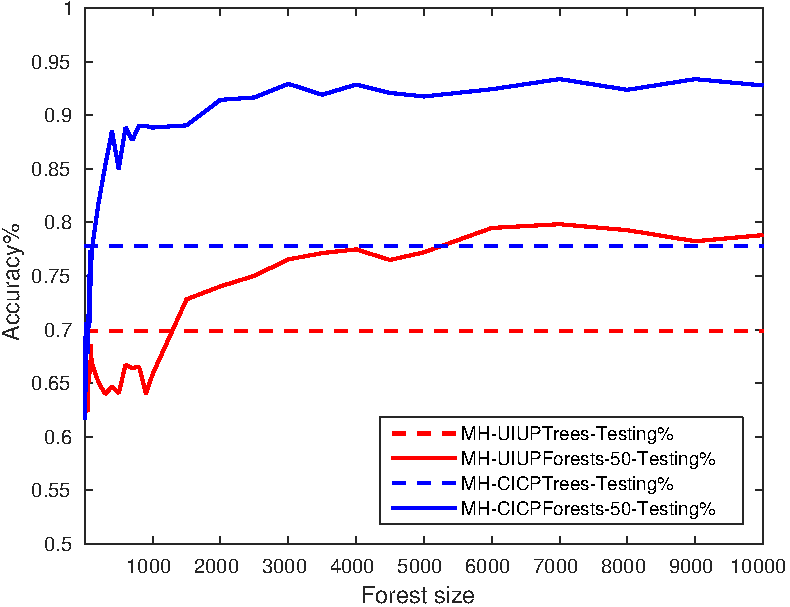
\includegraphics[width=\textwidth]{figs/PLPTF/Forests/MushroomDownsampled_Forests_MH.pdf}
  	\caption{Mushroom}
		\label{fig:Mush4}
	\end{subfigure}
  \begin{subfigure}[b]{0.3\textwidth}
		\centering
  	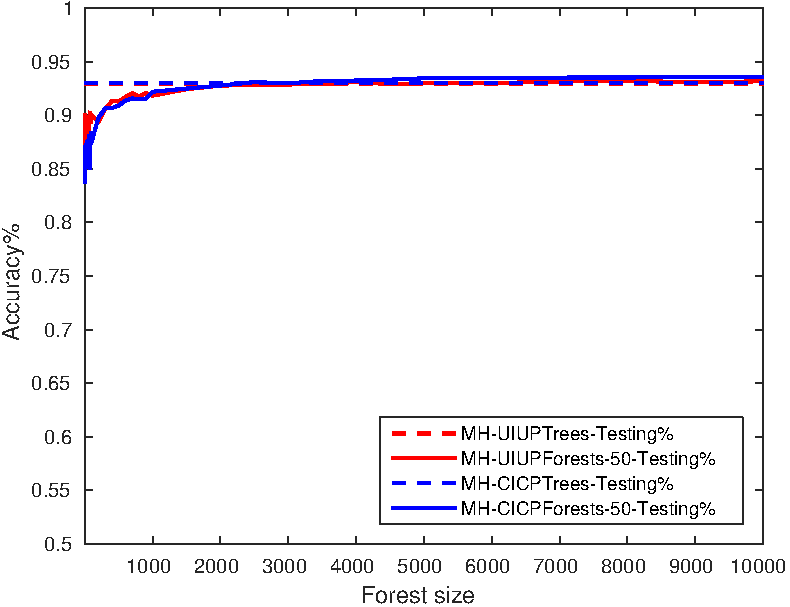
\includegraphics[width=\textwidth]{figs/PLPTF/Forests/NurseryDownsampledFurther_Forests_MH.pdf}
  	\caption{Nursery}
		\label{fig:N4}
	\end{subfigure}
  \begin{subfigure}[b]{0.3\textwidth}
		\centering
  	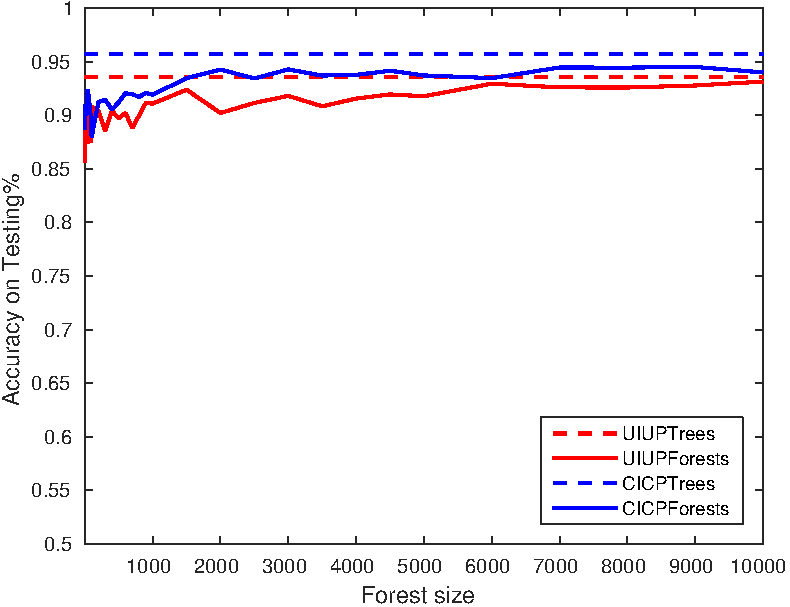
\includegraphics[width=\textwidth]{figs/PLPTF/Forests/SpectHeartDownsampledFurther_Forests_MH.pdf}
  	\caption{SpectHeart}
		\label{fig:S4}
	\end{subfigure}
  \\
  \begin{subfigure}[b]{0.3\textwidth}
		\centering
  	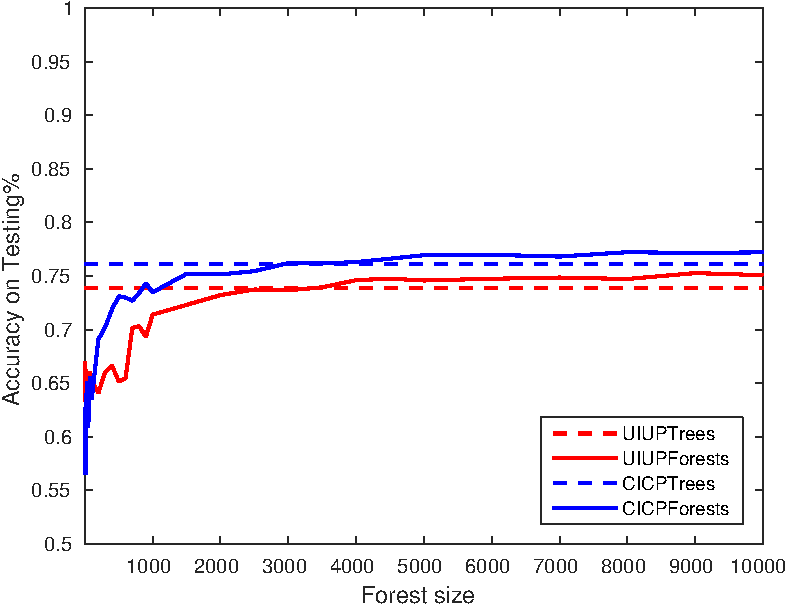
\includegraphics[width=\textwidth]{figs/PLPTF/Forests/TicTacToe_Forests_MH.pdf}
  	\caption{TicTacToe}
		\label{fig:T4}
	\end{subfigure}
  \begin{subfigure}[b]{0.3\textwidth}
		\centering
  	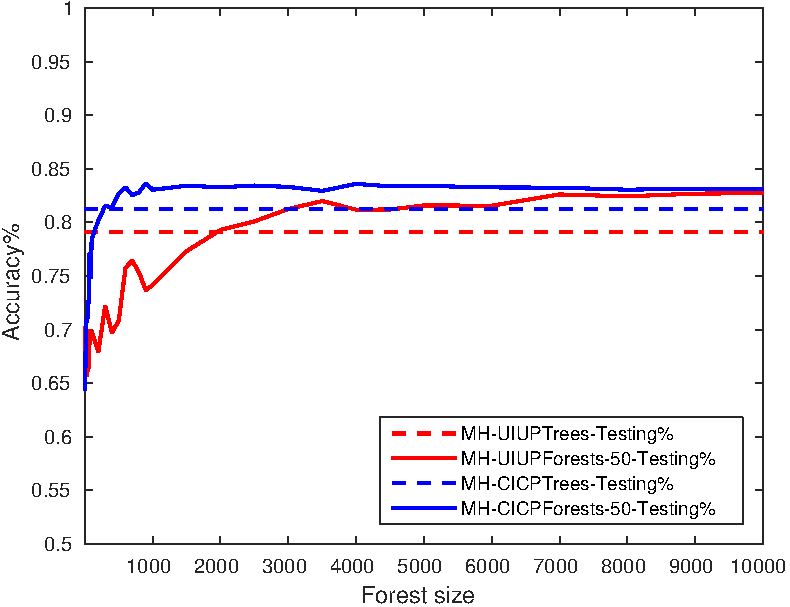
\includegraphics[width=\textwidth]{figs/PLPTF/Forests/VehicleDownsampledFurther_Forests_MH.pdf}
  	\caption{Vehicle}
		\label{fig:V4}
	\end{subfigure}
  \begin{subfigure}[b]{0.3\textwidth}
		\centering
  	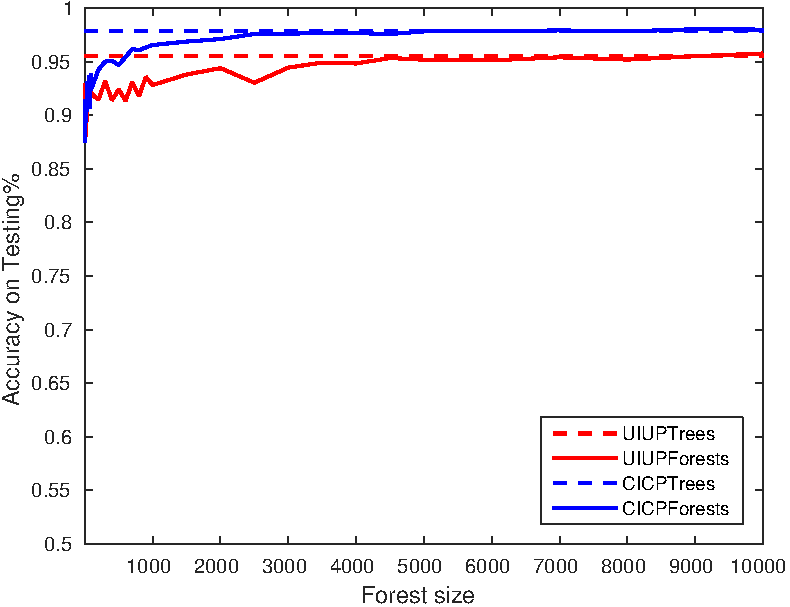
\includegraphics[width=\textwidth]{figs/PLPTF/Forests/WineDownsampled_Forests_MH.pdf}
  	\caption{Wine}
		\label{fig:W4}
	\end{subfigure}

  \caption{Forests of UIUP trees vs. forests of CICP trees}
  \label{fig:forests2}
\end{figure*}

What we have learned from \figref{forests2}:
\begin{enumerate}
	\item CICP forests surpass CICP trees on all but one dataset: SPECTHeart.
	\item UIUP forests surpass CICP trees on 4 datasets, and fall short on the others.
	\item CICP forests dominate UIUP forests on 10 datasets, and perform very close on
				the other 2.
\end{enumerate}


\section{Conclusion and Future Work}
In this paper, we reviewed different classifications of PLP-trees,
and introduced \tit{partial lexicographic preference forests},
or \tit{PLP-forests}, to reduce the high variance of PLP-trees.
To support experimentation, we have constructed a preference
learning library from existing reservoir of classification
datasets.
To this end, we implemented an \tit{exact} learner using
\tit{answer-set programming}, and an \tit{approximation}
learner using a straightforward greedy heuristic.
Our empirical results on PLP-trees show that the language offers
high accuracy, mostly higher than decision trees when training samples
are small.
For PLP-forests, we have observed improvements, significant in some cases,
from single tree models.

Looking into the future, we are interested in expanding our preference
learning library by creating real-work datasets through
conducting experiments involving human subjects.
We also plan to implement and experiment with other aggregators
for PLP-forests, and compare with our results using
the desirable and intuitive majority rule.


%Note the copyright notice at the end of each chapter.
\copyrightnotice

\chapter{Aggregating Lexicographic Preference Trees\label{ch:aggLP}}
%\paragraph{\bf Abstract.}
%\keywords{conditionally lexicographic preferences, social choice theory,
%positional scoring voting rules, answer set programming}
Aggregating \emph{votes} --- preference orders over \emph{candidates} 
or \emph{alternatives} --- is a fundamental problem of decision theory 
and social choice. We study this problem in the setting when 
alternatives are described as tuples of values of attributes. Such spaces of 
alternatives are called \emph{combinatorial}. They are characterized by 
large sizes that make explicit enumerations of alternatives from the most 
to the least preferred infeasible. Instead, typically votes are specified 
implicitly 
in terms of some compact and intuitive preference representation mechanism. 
In our work, we assume that votes are given as \textit{lexicographic 
preference trees} and consider two preference-aggregation problems, the 
\emph{winner} problem and the \emph{evaluation} problem. We study them 
under the assumption that \textit{positional scoring rules} (such as 
$k$-approval and Borda) are used for aggregation. We develop computational 
complexity results for these two problems. We also propose computational 
methods to solve 
them. They are based on encodings of the problems in \textit{Answer-Set 
Programming} and as instances of the \textit{Weighted Partial Maximum 
Satisfiability} problem, and exploit off-the-shelf solvers available for 
these two formalisms. Finally, we present results of an experimental study 
of the effectiveness of these methods.

\section{Introduction}
Preferences are an essential component of decision making, social choice,
knowledge representation, and constraint satisfaction. Fundamental 
problems of preference reasoning are to \emph{aggregate} individual 
preference orders of a group of agents (the \emph{votes} of agents in 
the group) into a consensus best candidate (the \emph{winner}), and to 
identify candidates with strong consensus support from the group 
(``good'' alternatives). These problems
have been studied extensively in social choice \cite{arrowhandbook}. 
Aggregation methods known as \emph{positional scoring rules}, which include
such well-known rules as plurality, $k$-approval and Borda, are
among the best understood and the most widely used ones.
 
When the number of alternatives is small, the simplest and most effective 
way to describe a preference order (a vote) is to enumerate the
alternatives from the most to the least preferred. Moreover, given a 
collection of such votes, for many aggregation rules, including all 
positional scoring rules, computing winners and ``good'' candidates is 
easy --- it can be done in polynomial time. The situation changes when
alternatives are characterized in terms of \emph{attributes} (or issues),
and are specified by tuples of attribute values. Spaces of such alternatives,
often called \emph{combinatorial domains}, are large. Indeed, the number 
of alternatives grows exponentially with the number of attributes. This
large size of combinatorial domains brings up two problems. First, it is
no longer feasible to describe votes by enumerating alternatives in the
order of preference. Thus, formalisms offering compact and intuitive
representations of votes are needed. Several such \emph{preference
formalisms} have been developed over the years including penalty logic 
\cite{de1994penalty}, possibilistic logic \cite{DuboisLP91}, conditional
preference networks (CP nets) \cite{bbdh03}, preference
trees \cite{fraser1994ordinal,liu2015reasoning}, 
and lexicographic preference trees \cite{booth:learningLP}.%
\footnote{Kaci \cite{Kaci:Pref} offers a comprehnsive discussion of 
preference formalisms.} Second, when votes are given as expressions in 
some preference formalism, computing the winner or a ``good'' candidate 
is no longer easy. In fact, it is known that for many preference formalisms 
these problems are NP-hard even when positional scoring rules are used 
to aggregate votes. \emph{Issue-by-attribute} aggregation addresses the
computational hardness problem but often leads to results different from 
those obtained by applying common voting rules \cite{fargier:ibi}.
  
In this chapter, we assume that votes are represented as \emph{lexicographic
preference trees}, or \emph{LP-trees}, for short~\cite{booth:learningLP},
and that they are aggregated by some simple positional scoring rules such 
as Borda, $k$-approval and a refinement of the latter, $(k,l)$-approval.
Given this setting, we study computing the best alternative, and the related 
problem to decide whether an alternative with the score exceeding a given 
threshold (a ``good'' alternative) exists. We refer to the former problem 
as the \emph{winner} problem and to the latter one as 
the \emph{evaluation} problem. In our setting, these problems are often
computationally hard. For Borda, the \emph{winner} problem is NP-hard and 
the \emph{evaluation} problem is NP-complete \cite{lang:aggLP}. For $k$-approval, 
for some specific values of $k$, both problems are in P but, for some other, 
they are NP-hard and NP-complete, respectively \cite{lang:aggLP}. Further,
when $(k,l)$-approval is used, for several values 
of $k$ and $l$, the problems are similarly hard.

Nevertheless, because the \emph{winner} and the \emph{evaluation}
problems arise in practice and the positional scoring rules
are common, computational tools for the two problems are needed. To 
develop such tools, we encode the problems in answer-set programming (ASP) 
\cite{mt99:stable,Niemela:1999} and weighted partial maximum satisfiability 
(WPM-SAT) \cite{ansotegui2010new,ansotegui2009solving}, and apply to the 
encodings the ASP solvers \emph{clingo} \cite{Gebser:clingo} and 
\emph{clingcon} \cite{Ostrowski:clingcon}, and a WPM-SAT solver \toulbar 
\cite{toulbar2}. We chose the two ASP solvers as they represent substantially
different approaches to computing answer sets. The \emph{clingo} solver is 
a native ASP solver developed along the lines of satisfiability solvers. 
The \emph{clingcon} solvers enhances \emph{clingo} with specialized 
treatment of some common classes of numeric constraints by delegating some 
reasoning tasks to a CP solver \emph{Gecode}~\cite{Schulte:gecode}. As 
problems we are considering involve numeric constraints, a comparison of 
the two solvers is of interest. We study all the resulting methods 
experimentally. To support the experimentation we propose and implement 
a method to randomly generate LP-trees of some restricted form.

The main contributions of our work are complexity results and algorithms 
for the \emph{winner} and the \emph{evaluation} problems when votes are 
specified as LP-trees. Specifically, we present new complexity results 
for the two problems for several positional scoring rules: $k$-approval 
(for specific values of $k$), variants of Borda, and $(k,l)$-approval 
(for specific combinations of values of $k$ and $l$). Next, we propose
algorithms for the two problems based on their ASP and WPM-SAT encodings 
and using ASP and WPM-SAT solvers. Finally, we provide an experimental 
evidence of the effectiveness of the proposed computational methods.


\section{Computing Ranks}
We now show how the \tit{rank} of an outcome in an LP-tree is computed.
As we consider positional scoring rules, the scores of an outcome
in an LP-tree or an LP-profile under these rules follow directly
from its rank in the tree.

Given an LP-tree $T$ and an outcome $o\in \CD(\cI)$,
the computation of the rank $r(T,o)$ of $o$ in $T$
is given in \algref{rank}, where $T'(x_j)$ is the 
left (more-preferred) subtree of $T'$, and
$T'(\obar{x_j})$ is the right (less-preferred)
subtree of $T'$. Note that in each case we need to
update the CPT's in the subtrees accordingly.
Clearly, \algref{rank} takes $O(p)$.
Conversely, it is also easy to compute the outcome
at a given rank in a tree.

\begin{algorithm}
\KwIn{LP-tree $T$ and outcome $o$}
\KwOut{the rank $r$ of $o$ in $T$}
	$r \lar 0$\;
	$T' \lar T$\;
	\For{$i \lar 1$ \KwTo $p$}{
		Let $X_j$ be the root attribute of $T'$ with preference $x_j > \obar{x_j}$\;
		\uIf{$o(X_j) = x_j$}{
			$T' \lar T'(x_j)$\;
		}
		\Else{
			$r \lar r + 2^{p-i}$\;
			$T' \lar T'(\obar{x_j})$\;
		}
	}
	\Return{$r$}
\caption{Compute the rank of an outcome in an LP-tree\label{alg:rank}}
\end{algorithm}

Now computing the scores of an outcome for the rules
$k$-approval, $(k,l)$-approval and Borda is straightforward.
We have the following.
\begin{enumerate}
	\item $k$-approval: $s_\kApp(T,o)=1$, if $r(T,o)<k$; $0$, otherwise.
	\item $(k,l)$-approval: $s_\klApp(T,o)=a$, if $r(T,o)<k$; $b$, if $k\leq r(T,o)<k+l$;
				$0$, otherwise.
	\item Borda: $s_\Borda(T,o)=m-r(T,o)-1$.
\end{enumerate}


\section{The Problems and Their Complexity}

We consider only \emph{effective implicit} positional scoring rules, 
that is, rules defined by an algorithm that given $m$ (the number of 
alternatives and, at the same time, the size of the scoring vector) 
and a rank $r$, $0\leq r\leq m-1$, (1) returns the value $w_r$ of 
the scoring vector, and (2) works in time polynomial in the sizes of 
$r$ and $m$. The rules $k$-approval, $(k,l)$-approval and Borda are examples 
of effective implicit positional scoring rules:

\begin{enumerate}
	\item $k$-approval: $w_\kApp(r,m)=1$, if $r<k$; $0$, otherwise.
	\item $(k,l)$-approval: $w_\klApp(r,m)=a$, if $r<k$; $b$, if $k\leq r<k+l$;
				$0$, otherwise.
	\item Borda: $w_\Borda(r,m)=m-r-1$.
\end{enumerate}

Let us fix an effective implicit positional scoring rule $\cD$ with the
scoring vector $w$. Given an LP profile $\cV$, the \emph{winner} problem for
$\cD$ consists of computing an alternative $o \in \cX$ with the maximum 
score $s_w(\cV,o)$. Similarly, given a profile $\cV$ and a positive integer 
$R$, the \emph{evaluation} problem for $\cD$ asks if there exists an 
alternative $o \in \mathcal{X}$ such that $s_{{w}}(\cV, o)\geq R$. In 
each case, $w$ is the scoring vector of $\cD$ for $m$ alternatives; we recall
that it is given implicitly in term of an algorithm that efficiently 
computes its entries.
     
We apply the voting rules listed above to profiles consisting of LP-trees or
\emph{LP profiles}, for short. We distinguish four classes of profiles,
UI-UP, UI-CP, CI-UP and CI-CP depending on the type of LP-trees they
consist of. 

\begin{remark}
The restriction to effective implicit positional scoring rules is 
essential in the context of combinatorial domains. It is because an 
explicit specification of the scoring vector has size equal to the 
number of alternatives and is exponential in the number of attributes. If 
it were to be given explicitly, it would have to be a part of input. 
The sheer size of the scoring vector would then make both the winner 
and the evaluation problems trivially solvable in polynomial time. 
However, most interesting positional scoring rules are effective 
implicit, which means that they can be described concisely as an 
algorithm (implicit) and at the same time provide a fast access to 
any weight in the scoring vector (effective). In this setting, the 
complexity of the winner and the evaluation problems is no longer 
obvious, and it is precisely this setting that models practical
situations, where scoring vectors are based on \emph{regular}
patterns.
\end{remark}


\subsection{$k$-Approval}
If $k=2^{p-1}$ the evaluation problem is in P for all four classes of 
profiles of LP-trees \cite{lang:aggLP}. However, if $k$ equals $2^{p-2}$
or $2^{p-3}$, the problem is NP-complete, again for all four types of 
profiles \cite{lang:aggLP} (in fact, the result holds for a larger set 
of values $k$, we refer for details to the paper by Lang et al. 
\cite{lang:aggLP}). Clearly, in each case where the evaluation problem 
is NP-complete, the winner problem is NP-hard.

We first show that the two problems are in P even when the deviation of
$k$ from $2^{p-1}$ is given by a polynomial in $p$. In other words, 
if $k=2^{p-1} + f(p)$ or $k=2^{p-1} - f(p)$, where $f(p)$ is a polynomial 
in $p$ such that $f(p)\geq 0$ for $p\geq 1$, both the winner and the 
evaluation problems for $k$-approval can be solved by polynomial time 
algorithms. The next two results address the two cases for $k$,
respectively.

\begin{thm}
\label{thm1}
Let $f$ be a polynomial such that $f(p)\geq 0$ for $p\geq 1$, and let
$k=2^{p-1}+f(p)$. Given 
a profile of $n$ LP-trees over $p$ binary attributes $X_1,\ldots,X_p$, the 
winner under $k$-approval can be computed in time polynomial in the
size of the profile.
\end{thm}
\begin{proof}
Let $P$ be a profile of $n$ LP-trees. The score $s_k(o)$ of an alternative
$o$ under $k$-approval in $P$ is given by 
\[
s_k(o) = s'(o)+s''(o),
\]
where $s'(o)$ is the score of $o$ under the $2^{p-1}$-approval (the number
of votes that place $o$ in the upper half of the order), and $s''(o)$ is the
number of votes that place $o$ as one of top $f(p)$ votes in the lower 
half (we omit references to the profile to simplify the notation).

To find the highest possible score $s'(o)$, we define $x_i=0$, if 
the number of votes with the root labeled with $X_i$ and with 0 preferred
to 1 is \emph{strictly} larger than the number of votes with the root 
labeled with $X_i$ with 1 preferred to 0. We define $x_i=1$ similarly.
If $x_i$ does not get set to 0 or 1, it is set to $u$ (undefined). We
call the resulting $p$-tuple a \emph{partial alternative} and denote 
it by $PA$. Since it is the root that decides whether an LP-tree 
contributes 1 to the score of an alternative, it is clear that any 
alternative consistent with $PA$ achieves the highest possible 
score under $2^{p-1}$-approval, that is, the highest possible $s'$-score.  
Finding this score, say $W'$, can then be accomplished by (1) finding
an alternative $o$ consistent with $PA$, and (2) finding its score $s'(o)$.
Clearly, both (1) and (2) together can be done in time bounded by a polynomial 
in the size of the profile.

Next, we consider $s''$. Let us denote by $A$ the set of all alternatives 
$o$ with $s''(o)>0$. To this end, it is enough
to find in each tree $T$ in $P$ alternatives with ranks $2^{p-1}+1,
\ldots, 2^{p-1}+f(p)$. Since finding an alternative of a given rank in 
an LP-tree can be accomplished in time polynomial in $p$, the set $A$ 
can indeed be computed in time polynomial in the size of the profile.

We now compute $s_k(o)$ for all alternatives in $A$. Given the size of
$A$, the task can be computed in time bounded by a polynomial in the size
of the profile. Let $W$ be the maximum of these scores achieved, say, by an
alternative $o$. If $W\geq W'$, then $o$ is a winning alternative (has 
the best score among those in $A$ and the score of any other alternative 
does not exceed $W'$). Otherwise, any alternative consistent with $PA$ 
can be taken for the winner (indeed, in such case, the highest possible 
score to achieve under $k$-approval is $W'$). 
\end{proof}

%\begin{cor}
	%Theorem \ref{thm1} holds for $k$-approval when 
	%$k=2^{p-1}+f(p)$, where $f(p)$ is a polynomial in $p$.
%\end{cor}

\begin{thm}
\label{thm2}
Let $f$ be a polynomial such that $f(p)\geq 0$ for $p\geq 1$, and let
$k=2^{p-1}-f(p)$. Given a profile of $n$ LP-trees over $p$ binary attributes 
$X_1,\ldots,X_p$, the winner under $k$-approval can be computed in time 
polynomial in the size of the profile.
\end{thm}
\begin{proof}
Let $P$ be a profile of $n$ LP-trees. Similarly as in the proof of the
previous result, the score $s_k(o)$ of an alternative $o$ under 
$k$-approval is given by
\[
s_k(o) = s'(o)-s''(o),
\]
where $s'(o)$ is the score of $o$ under the $2^{p-1}$-approval (the number
of votes that place $o$ in the upper half of the order), and $s''(o)$ is the
number of votes that place $o$ as one of the bottom $f(p)$ votes in the upper
half (we omit references to the profile to simplify the notation).

Let us denote by $A$ the set of alternatives $o$ such that $s''(o)>0$.
As before, this set can be computed in time bounded by a polynomial in 
the size of the profile. Let $t=|A|$. If every alternative is in $A$
(that is, $t=2^p$), then, we compute an alternative with the highest
$k$-approval score by computing the scores of all alternatives in $A$
and selecting the one with the highest score. Since the size of $A$ is
polynomial in the size of the profile, the task takes polynomial time
(in the size of the profile).

The case when $t< 2^p$ is harder. To address it, let us assume that we 
have computed the set $B$ of top $t+1$ alternatives according to their 
$s'$-score (the $2^{p-1}$-approval score). Next, let $o$ be an alternative 
in $B$ with the maximum $k$-approval score $s_k(o)$.

We claim that $o$ is also an alternative with the maximum $k$-approval 
score over all alternatives. Indeed, consider an arbitrary alternative 
$o'$. If $o'\in B$, then $s_k(o)\geq s_k(o)$ (by the way $o$ was selected). 
Thus, let us assume that $o'\notin B$. Since $|B|> |A|$, there is at least 
one alternative $o''\in B\setminus A$. As $o''\in B$, $s_k(o)\geq s_k(o'')$.
Moreover, as $o''\notin A$, $s_k(o'')=s'(o'')-s''(o'')=s'(o'')$. Finally,
since $o''\in B$ and $o'\notin B$, $s'(o'')\geq s'(o')$. Combining these 
three inequalities, we obtain that $s_k(o) \geq s'(o')$. Since $s'(o')\geq 
s'(o')-s'(o'')=s_k(o')$, we get $s_k(o)\geq s_k(o')$. Thus, the claim follows.

Clearly, $t+1$ is bounded by a polynomial in the size of the profile. 
Thus, once $B$ is computed, finding an alternative in $B$ with the 
highest $k$-approval score can be done in time polynomial in the size 
of the profile. To complete the proof, it suffices then to show how to 
compute $B$ in polynomial time. 

To this end, for each $i=1,\ldots,p$, we set $d_i$ to the absolute value 
of the difference between the numbers of trees in the profile with the root 
labeled with $X_i$ and with 0 (respectively, with 1) as the preferred value. 
We also select any alternative that has the highest $s'$-score (we 
explained in the previous proof how to compute it in polynomial time)
and denote it by $o$. Finally, we compute the score of $o$ and denote it 
by $W'$ (to use the notation from the previous proof). 

Let $S\subseteq\{1,\ldots,p\}$ be a set of attribute indices, and let $o_S$
be an alternative obtained from $o$ by ``flipping'' its values in 
positions in $S$. Every alternative can be described in these terms.
This is useful as the $s'$-score of $o_S$ is easy to compute. Namely, 
we have
\[
s'(o_S) = W' - w(S),
\]
where $w(S)=\sum_{i\in S} d_i$ is the \emph{weight} of $S$.

It follows that $B$ is determined by $t+1$ smallest-weight subsets 
of $\{1,\ldots,p\}$. We will now show that given a list $D=\{d_1,d_2,
\ldots,d_p\}$ and an integer $t$, the $t+1$ smallest-weight subsets 
of $\{1,\ldots,p\}$ can be computed in time bounded by a polynomial in
$p$ and $t$.  

Let $r$ be an integer such that $2^r\geq t+1$. Let us assume that $L_r$ is
the set of $t+1$ smallest-weight subsets of $\{1,\ldots,r\}$. Let 
\[
L'_{r+1}=L_r \cup \{S\cup \{r+1\}\colon S\in L_r\}
\]
and let $L_{r+1}$ be the collection of $t+1$ smallest-weight subsets $S$
of $L'_{r+1}$. We will show that $L_{r+1}$ contains $t+1$ smallest-weight 
subsets $S$ of $\{1,\ldots,r+1\}$. Indeed, let us consider $S\subseteq\{1,
\ldots,r+1\}$ such that $S\notin L'_{r+1}$. If $S\subseteq \{1,\ldots, r\}$,
then $S\notin L_r$. Thus, $w(S)\geq w(S')$, for every $S'\in L_r$.
If $r+1\in S$, then $S=R\cup\{r+1\}$, for some $R\subseteq \{1,\ldots,r\}$.
Since $S\notin L'_{r+1}$, $R\notin L_r$. Thus, $w(R)\geq w(R')$, for every
$R'\in L_r$ and so, $w(S)\geq w(R'\cup\{r+1\})$ for all $R'\in L_r$.
In each case, it follows that there are at least $t+1$ sets $S'$ in 
$L'_{r+1}$ such that $w(S)\geq w(S')$. Thus for every $S'\in L_{r+1}$, 
$w(S)\geq w(S')$. 

Clearly, the list $L_p$ consists of $t+1$ smallest weight subsets of
$\{1,\ldots,p\}$. Thus, it can be taken for $B$. To compute it, we first
find the smallest $r$ such that $2^r\geq t+1$ (such an $r$ exists as
we are now considering the case when $t < 2^p$). We then construct the 
collection $U$ of all subsets of $\{1,\ldots, r\}$ (this collection 
has no more than $2t$ elements and can be constructed in time bounded 
by a polynomial in $p$ and $t$). Next, we construct $L_r$ by selecting 
from $U$ its $t+1$ smallest-weight elements. Since $|U|\leq 2t$, this task
also can be accomplish in polynomial time (in $p$ and $t$).

From now on, we construct $L_{r+1},L_{r+2},\ldots L_p$ recursively, as 
described above. Since each step of the construction can be accomplished
by the same polynomial-time algorithm (form the collection $L'$, select
its $t+1$ smallest-weight elements to form the next $L$), and since
the number of steps is bounded by $p$, the total time needed to construct
$B$ ($L_p$) is bounded by a polynomial in $p$ and $t$.  
\end{proof}

%\begin{cor}
	%Theorem \ref{thm2} holds for $k$-approval when 
	%$k=2^{p-1}-f(p)$, where $f(p)$ is a polynomial in $p$.
%\end{cor}

For the $k$-approval rule, we summarize the results in \tblref{kApp_comp},
where \tblref{kApp_comp_a} presents our results as discussed above,
and results in \tblref{kApp_comp_b} were obtained by others
\cite{lang:aggLP}.
\begin{table}
	\centering
  \begin{subfigure}[b]{0.5\textwidth}
		\centering
		\begin{tabular}[0.5\textwidth]{ | c | c | c | }
		  \hline
		    & UP & CP \\
		  \hline
		  UI & P & P \\
		  \hline
		  CI & P & P \\
		  \hline
		\end{tabular}
		\caption{$k=2^{p-1}\pm f(p)$}
		\label{tbl:kApp_comp_a}
	\end{subfigure}%
  \begin{subfigure}[b]{0.5\textwidth}
		\centering
		\begin{tabular}[0.5\textwidth]{ | c | c | c | }
		  \hline
		    & UP & CP \\
		  \hline
		  UI & NPC & NPC \\
		  \hline
		  CI & NPC & NPC \\
		  \hline
		\end{tabular}
		\caption{$k=c\cdot 2^{p-M}$ and $k \not = 2^{p-1}$}
		\label{tbl:kApp_comp_b}
	\end{subfigure}
	\caption{$k$-Approval}
	\label{tbl:kApp_comp}
\end{table}


\subsection{$(k,l)$-Approval}
%In the most restrictive case of UI-UP profiles, the evaluation
%problem for the Borda rule is in P and it is NP-complete for the three
%other classes of profiles \cite{lang:aggLP}. The picture for the 
%the $k$-approval rule is more complicated. If $k=2^{p-1}$ the evaluation
%problem is in P for all four classes of profiles. 
%However, if $k$ equals $2^{p-2}$ or $2^{p-3}$,
%the problem is NP-complete, again for all four LP profile types
%\cite{lang:aggLP} (in fact, the result holds for a larger set of values
%$k$, we refer for details to Lang et al. \cite{lang:aggLP}).
%Clearly, in each case where the evaluation problem is NP-complete, the winner
%problem is NP-hard.

To the best of our knowledge, the complexity of the 2-valued $(k,l)$-approval 
rule has not been studied. It is evident that $(k,l)$-approval is an effective
implicit positional scoring rule. It turns out that, as with the $k$-approval 
rule, for some values of the parameters, the evaluation problem for 
$(k,l)$-approval is NP-complete. Preliminary results we obtained 
have been published \cite{conf/adt13/LiuT}.
We describe cases where $k=l=2^{p-c}$,
where $c$ is a constant and $1<c<p$.
%We describe two such cases here: (1) $k=l=2^{p-2}$, and (2) $k=l=2^{p-3}$.
%We note that if $a=1$ and $b=0$, case (1) reduces to $2^{p-2}$-approval 
%and case (2) to $2^{p-3}$-approval. 
If $a=2$ and $b=1$, we refer to the rule 
$(2^{p-2},2^{p-2})$-approval as $2K$-$approval$.
We show proof of NP-completeness of the evaluation problem for
$(2^{p-2},2^{p-2})$-approval.

\begin{thm}
The following problem is NP-complete: decide for a given UI-UP profile 
$\cV$ and an integer $R$ whether there is an alternative $o$ such that 
$s_w(\cV,o) \geq R$, where $w$ is the scoring vector of the $(2^{p-2},
2^{p-2})$-approval rule.
\end{thm}
\begin{proof}
        We can guess in polynomial time an alternative $o \in \mathcal{X}$ and
        verify in polynomial time that $S_w(\cV, o) \geq R$ (this is possible 
because $(k,l)$-approval is an effective implicit scoring rule; the score of an alternative in
a vote can be computed in polynomial time once its position is known, and 
the position can be computed in polynomial time be traversing the tree 
representing the vote).  So membership in NP follows.
        Hardness follows from a polynomial reduction from the
        problem $2$\textit{-MINSAT}\footnote{Let $N$ be an integer ($N>1$),
				the $N$-MINSAT problem
        is defined as follows.  Given a set $\Phi$ of $n$ $N$-clauses
        $\{ c_1,\ldots,c_n \}$ over a set of propositional variables
        $\{ X_1,\ldots,X_p \}$,
        and a positive
        integer $l$ ($l \leq n$), decide whether there is a truth assignment that
        satisfies at most $l$ clauses in $\Phi$.} \cite{Kohli:2maxsat}, which is NP-complete.
        Given an instance $\langle \Phi, l \rangle$ of the 2-MINSAT problem,
we construct the set of attributes
        $\cI$, the set of alternatives $\mathcal{X}$, the profile $\cV$ and the threshold $R$.

        Important observations are that $o$ is among the
				top first quarter of alternatives in an LP-tree 
$\mathcal{L}$ if and only if the top two most important attributes in $\mathcal{L}$ 
are both assigned the preferred values; and that $o$ is among the second top 
quarter of alternatives if and only if the most important attribute is assigned 
the preferred value and the second most important one is assigned the 
non-preferred one.
				
\noindent
(1). We define $\cI = \{ X_1,\ldots,X_p \}$, where $X_i$s are all propositional
letters occurring in $\Phi$. Clearly, the set $\cX$ of all alternatives over 
$\cI$ coincides with the set of truth assignments of variables in $\cI$.

\noindent
(2). Let $\Psi$ be the set of formulas $\{ \neg c_i:c_i \in \Phi \}$.  
For each $\neg c_i \in \Psi$, we build $a+b$ UI-UP trees. For instance, 
if $\neg c_i = X_2 \land \neg X_4$, then we proceed as follows.
Firstly, we build $a-b$ duplicate trees shown in
\figref{proof1}. Secondly, we construct $b$ duplicate trees shown in
\figref{proof2}. Thirdly, we build another $b$ duplicate trees shown in
\figref{proof3}. (In all three figures we only indicate the top two attributes 
since the other attributes can be ordered arbitrarily.) Denote by $\cV_i$ the 
set of these $a+b$ UI-UP trees for formula $\neg c_i$. Then $\cV = \bigcup_{1 
\leq i \leq n} \cV_i$ and has $n*(a+b)$ votes.

\noindent
(3). Finally, we set $R=(n-l)*(a^2-ab+b^2)+l*ab$.

        Note that the construction of $\cV$ ensures that if $o \models \neg c_i$, $S_w(\cV_i, o)=
        a^2-ab+b^2$; 
				otherwise if $o \not \models \neg c_i$, $S_w(\cV_i, o)=ab$.  We have $a^2-ab+b^2 > ab$ since 
        $(a-b)^2 > 0$.  Hence, there is an assignment 
				satisfying at most $l$ clauses in $\Phi$ 
if and only if there is an assignment satisfying 
				at least $n-l$ formulas in $\Psi$ 
if and only if there is an alternative with the $(2^{p-2},2^{p-2})$-approval
score of at least $R$ given the profile $\cV$. 

Since the first equivalence is clear, it suffices to show the second.
Let $o$ be an assignment satisfying $l'$ formulas in $\Psi$. 
We have $S_w(\cV, o) - R = (l'+l-n)*(a^2-ab+b^2)+(n-l'-l)*ab
= (l'+l-n)*(a^2-2ab+b^2) = (l'+l-n)*(a-b)^2$.
It follows that $S_w(\cV, o) \geq R$ if and only if $l'+l-n \geq 0$
if and only if $l' \geq n-l$.  
\end{proof}

\begin{figure*}[!ht]
  \centering
  \setlength{\tabcolsep}{0mm}
  \begin{tabular}{c}
  \begin{subfigure}[b]{0.25\textwidth}
    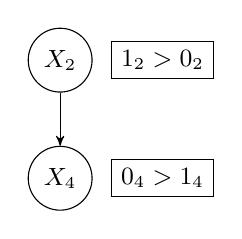
\begin{tikzpicture}[->,>=stealth',node distance=1.5cm,main node/.style={circle,draw,font=\small}]
      \node[main node] (1) {$X_2$};
      \node[rectangle,draw] at (1.3,0) {$1_2 > 0_2$};

      \node[main node] (2) [below of=1] {$X_4$};
      \node[rectangle,draw] at (1.3,-1.5) {$0_4 > 1_4$};

      \path[]
        (1) edge (2);
    \end{tikzpicture}
    \caption{}
    \label{fig:proof1}
  \end{subfigure}

  \begin{subfigure}[b]{0.25\textwidth}
    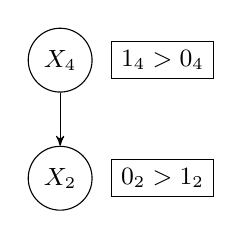
\begin{tikzpicture}[->,>=stealth',node distance=1.5cm,main node/.style={circle,draw,font=\small}]
      \node[main node] (1) {$X_4$};
      \node[rectangle,draw] at (1.3,0) {$1_4 > 0_4$};

      \node[main node] (2) [below of=1] {$X_2$};
      \node[rectangle,draw] at (1.3,-1.5) {$0_2 > 1_2$};

      \path[]
        (1) edge (2);
    \end{tikzpicture}
    \caption{}
    \label{fig:proof2}
  \end{subfigure}

  \begin{subfigure}[b]{0.25\textwidth}
    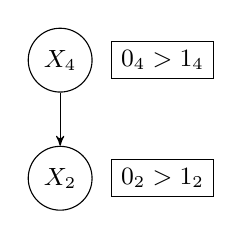
\begin{tikzpicture}[->,>=stealth',node distance=1.5cm,main node/.style={circle,draw,font=\small}]
      \node[main node] (1) {$X_4$};
      \node[rectangle,draw] at (1.3,0) {$0_4 > 1_4$};

      \node[main node] (2) [below of=1] {$X_2$};
      \node[rectangle,draw] at (1.3,-1.5) {$0_2 > 1_2$};

      \path[]
        (1) edge (2);
    \end{tikzpicture}
    \caption{}
    \label{fig:proof3}
  \end{subfigure}
  \end{tabular}

  \caption{UI-UP LP-trees}
  \label{fig}
\end{figure*}

This hardness proof applies to more general classes of LP-trees, namely 
UI-CP, CI-UP and CI-CP, and the winner problem for those cases is NP-hard.
%In general, the evaluation problem according to $(2^{p-c},2^{p-c})$-approval,
%where $c$ is a constant and $1<c<p$, for the four 
%classes of LP-trees is NP-complete. In each case, the hardness follows from
%from an NP-complete version of the \textit{c-MINSAT} problem. 
Below we show the proof of NP-completeness of the evaluation problem
for $(2^{p-3},2^{p-3})$-approval.

\begin{thm}
	Let $w$ be the scoring vector $(a,\ldots,a, b,\ldots,b, 0\ldots,0)$ with the numbers of 
	$a$'s and $b$'s each equal to $2^{p-3}$.  The problem of deciding for a given UI-UP profile 
	$V$ and an integer $R$ whether there is an alternative
	$o$ such that $s_w(V,o) \geq R$ is NP-complete.
\end{thm}
\begin{proof}
  We can guess in polynomial time an alternative $o \in \mathcal{X}$ and 
  verify in polynomial time that $S_w(V, o) \geq R$.  So membership in NP follows.

  Hardness follows from a polynomial reduction from the NP-complete 
  problem 3\textit{-MAXSAT} \cite{Papadimitriou:1988}.
  Let $\Phi$ be a set of $n$ 3-clauses $\{ c_1,\ldots,c_n \}$ over $\{ X_1,\ldots,X_p \}$, 
  $l$ an integer such that $0 \leq l \leq n$.
  Given an instance of 3\textit{-MAXSAT} $I=\langle \Phi, l \rangle$, we construct the set of attributes 
  $X$, the set of alternatives $\mathcal{X}$, the profile $V$ and the threshold $R$ as follows.

  (1) $X = \{ X_1,\ldots,X_p \}$.  $\mathcal{X}$ is then the set of 
      all alternatives over $X$.

  (2) Let $\Psi$ be the set of formulas $\{ \neg c_i:c_i \in \Phi \}$.  For each 
      $\neg c_i \in \Psi$, we build multiple UI-UP LP-trees.  Assume there is $c_i = 
      \neg X_1 \vee \neg X_2 \vee \neg X_3 \in \Phi$. Then we have $\neg c_i = X_1 \wedge 
      X_2 \wedge X_3 \in \Psi$.  For $\neg c_i$, we build $a^2$ duplicate trees of 
      type~\ref{fig:1}, $a^2$ duplicate trees of type~\ref{fig:2}, $a^2$ duplicate 
      trees of type~\ref{fig:3}, $a^2$ duplicate trees of type~\ref{fig:4}, 
      $a^2-ab$ duplicate trees of type~\ref{fig:5}, 
      $a^2-ab$ duplicate trees of type~\ref{fig:6} and 
      $(a-b)^2$ duplicate trees of type~\ref{fig:7}. 
      Denote by $V_i$ the set of $7a^2-4ab+b^2$ UI-UP LP-trees for formula 
      $\neg c_i$.  Then $V = \bigcup_{1 \leq i \leq n} V_i$ and has 
      $n*(7a^2-4ab+b^2)$ votes.

  (3) We set $R = a^3*l+(3a^2b-3ab^2+b^3)*(n-l)$.

  Note that the construction of $V$ ensures that if $o \models \neg c_i$, $S_w(V_i, o)=
  3a^2b-3ab^2+b^3$; 
  otherwise if $o \not \models \neg c_i$, $S_w(V_i, o)=a^3$.  
  We have $a^3 > 3a^2b-3ab^2+b^3$ since 
  $a^3-(3a^2b-3ab^2+b^3)=(a-b)^3 > 0$.
  Therefore, there is an assignment 
  satisfying at least $l$ clauses in $\Phi$ \textit{iff} there is an assignment falsifying 
  at least $l$ formulas in $\Psi$ \textit{iff} there is an alternative scoring at least 
  $R$ with respect to profile $V$ and our scoring vector $w$.
	Since the first equivalence is obvious, it suffices to show the second one.

	($\Rightarrow$) Assume $o$ is the assignment that falsifies $l'$ ($l' \geq l$) formulas 
	in $\Psi$, its score $S_w(V, o) = a^3*l'+(3a^2b-3ab^2+b^3)*(n-l')$.
	Then $S_w(V, o)-R = a^3*(l'-l)+(3a^2b-3ab^2+b^3)*(l-l') = 
	a^3*(l'-l)-(3a^2b-3ab^2+b^3)*(l'-l) = 
	(a-b)^3*(l'-l) \geq 0$.  Thus, $S_w(V, o) \geq R$.

	($\Leftarrow$) Suppose $o$ is the alternative such that $S_w(V, o) \geq R$.
	Prove by contradiction.  Assume $o$ falsifies $l'$ formulas in $\Psi$ 
	and $l' < l$. Then $S_w(V, o)-R = (a-b)^3*(l'-l) < 0$, which implies that
	$S_w(V, o) < R$.  Contradiction!  Therefore, it must be that $l' \geq l$.

\end{proof}

\begin{figure*}[!ht]
  \centering
  \setlength{\tabcolsep}{0mm}
  \begin{tabular}{c}
  \begin{subfigure}[b]{0.25\textwidth}
    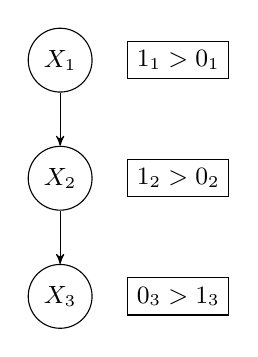
\begin{tikzpicture}[->,>=stealth',node distance=1.5cm,main node/.style={circle,draw,font=\small}]
      \node[main node] (1) {$X_1$};
      \node[rectangle,draw] at (1.5,0) {$1_1 > 0_1$};
    
      \node[main node] (2) [below of=1] {$X_2$};
      \node[rectangle,draw] at (1.5,-1.5) {$1_2 > 0_2$};
    
      \node[main node] (3) [below of=2] {$X_3$};
      \node[rectangle,draw] at (1.5,-3) {$0_3 > 1_3$};

      \path[]
        (1) edge (2)
        (2) edge (3);
    \end{tikzpicture}
    \caption{}
    \label{fig:1}
  \end{subfigure}
  \begin{subfigure}[b]{0.25\textwidth}
    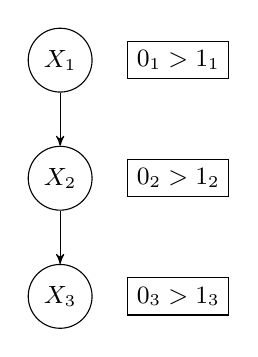
\begin{tikzpicture}[->,>=stealth',node distance=1.5cm,main node/.style={circle,draw,font=\small}]
      \node[main node] (1) {$X_1$};
      \node[rectangle,draw] at (1.5,0) {$0_1 > 1_1$};
    
      \node[main node] (2) [below of=1] {$X_2$};
      \node[rectangle,draw] at (1.5,-1.5) {$0_2 > 1_2$};
    
      \node[main node] (3) [below of=2] {$X_3$};
      \node[rectangle,draw] at (1.5,-3) {$0_3 > 1_3$};

      \path[]
        (1) edge (2)
        (2) edge (3);
    \end{tikzpicture}
    \caption{}
    \label{fig:2}
  \end{subfigure}
  \begin{subfigure}[b]{0.25\textwidth}
    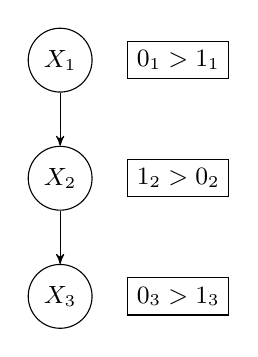
\begin{tikzpicture}[->,>=stealth',node distance=1.5cm,main node/.style={circle,draw,font=\small}]
      \node[main node] (1) {$X_1$};
      \node[rectangle,draw] at (1.5,0) {$0_1 > 1_1$};
    
      \node[main node] (2) [below of=1] {$X_2$};
      \node[rectangle,draw] at (1.5,-1.5) {$1_2 > 0_2$};
    
      \node[main node] (3) [below of=2] {$X_3$};
      \node[rectangle,draw] at (1.5,-3) {$0_3 > 1_3$};

      \path[]
        (1) edge (2)
        (2) edge (3);
    \end{tikzpicture}
    \caption{}
    \label{fig:3}
  \end{subfigure}
  \begin{subfigure}[b]{0.25\textwidth}
    \begin{tikzpicture}[->,>=stealth',node distance=1.5cm,main node/.style={circle,draw,font=\small}]
      \node[main node] (1) {$X_1$};
      \node[rectangle,draw] at (1.5,0) {$1_1 > 0_1$};
    
      \node[main node] (2) [below of=1] {$X_2$};
      \node[rectangle,draw] at (1.5,-1.5) {$0_2 > 1_2$};
    
      \node[main node] (3) [below of=2] {$X_3$};
      \node[rectangle,draw] at (1.5,-3) {$0_3 > 1_3$};

      \path[]
        (1) edge (2)
        (2) edge (3);
    \end{tikzpicture}
    \caption{}
    \label{fig:4}
  \end{subfigure}
  \\
  \begin{subfigure}[b]{0.25\textwidth}
    \begin{tikzpicture}[->,>=stealth',node distance=1.5cm,main node/.style={circle,draw,font=\small}]
      \node[main node] (1) {$X_1$};
      \node[rectangle,draw] at (1.5,0) {$0_1 > 1_1$};
    
      \node[main node] (2) [below of=1] {$X_3$};
      \node[rectangle,draw] at (1.5,-1.5) {$1_3 > 0_3$};
    
      \node[main node] (3) [below of=2] {$X_2$};
      \node[rectangle,draw] at (1.5,-3) {$0_2 > 1_2$};

      \path[]
        (1) edge (2)
        (2) edge (3);
    \end{tikzpicture}
    \caption{}
    \label{fig:5}
  \end{subfigure}
  \begin{subfigure}[b]{0.25\textwidth}
    \begin{tikzpicture}[->,>=stealth',node distance=1.5cm,main node/.style={circle,draw,font=\small}]
      \node[main node] (1) {$X_1$};
      \node[rectangle,draw] at (1.5,0) {$1_1 > 0_1$};
    
      \node[main node] (2) [below of=1] {$X_3$};
      \node[rectangle,draw] at (1.5,-1.5) {$1_3 > 0_3$};
    
      \node[main node] (3) [below of=2] {$X_2$};
      \node[rectangle,draw] at (1.5,-3) {$0_2 > 1_2$};

      \path[]
        (1) edge (2)
        (2) edge (3);
    \end{tikzpicture}
    \caption{}
    \label{fig:6}
  \end{subfigure}
  \begin{subfigure}[b]{0.25\textwidth}
    \begin{tikzpicture}[->,>=stealth',node distance=1.5cm,main node/.style={circle,draw,font=\small}]
      \node[main node] (1) {$X_2$};
      \node[rectangle,draw] at (1.5,0) {$1_2 > 0_2$};
    
      \node[main node] (2) [below of=1] {$X_3$};
      \node[rectangle,draw] at (1.5,-1.5) {$1_3 > 0_3$};
    
      \node[main node] (3) [below of=2] {$X_1$};
      \node[rectangle,draw] at (1.5,-3) {$0_1 > 1_1$};

      \path[]
        (1) edge (2)
        (2) edge (3);
    \end{tikzpicture}
    \caption{}
    \label{fig:7}
  \end{subfigure}

  \end{tabular}
  \caption{UI-UP LP-trees}
  \label{fig}
\end{figure*}

For the $(k,l)$-approval rule, we capture our results as \tblref{klApp_comp}.

\begin{table}
	\centering
  \begin{subfigure}[b]{0.5\textwidth}
		\centering
		\begin{tabular}[0.5\textwidth]{ | c | c | c | }
		  \hline
		    & UP & CP \\
		  \hline
		  UI & P & P \\
		  \hline
		  CI & P & P \\
		  \hline
		\end{tabular}
		\label{tbl:klApp_comp_a}
		\caption{$k=l=2^{p-1}$}
	\end{subfigure}%
  \begin{subfigure}[b]{0.5\textwidth}
		\centering
		\begin{tabular}[0.5\textwidth]{ | c | c | c | }
		  \hline
		    & UP & CP \\
		  \hline
		  UI & NPC & NPC \\
		  \hline
		  CI & NPC & NPC \\
		  \hline
		\end{tabular}
		\label{tbl:klApp_comp_b}
		\caption{$k=l=2^{p-c}$ and $1 < c < p$}
	\end{subfigure}
	\caption{$(k,l)$-Approval}
	\label{tbl:klApp_comp}
\end{table}


\subsection{$b$-Borda}
By \emph{$b$-Borda} we mean a positional scoring rule with the scoring 
vector $\langle b,b-1,b-2,\ldots\rangle$. Let $m=2^p$ denote the number 
of alternatives in $\cX(\cI)$ (where, as always, $\cI =\{X_1,\ldots, 
X_p\}$). If $b \geq 2^p-1$, $b$-Borda can be reduced to the (standard) 
Borda rule. 
In the most restrictive case of UI-UP profiles, the evaluation problem 
for the Borda rule is in P, and it is NP-complete for the three other 
classes of profiles \cite{lang:aggLP}. 

When $b < 2^p-1$, we show that for some values
of $b$, the winner and the evaluation problems under the 
$b$-Borda rules are NP-hard and NP-complete, respectively, no matter
what the type of LP-trees used in profiles. The cases of UI-CP, CI-UP
and CI-CP trees are handled by a fairly direct reduction from the 
corresponding problems under the Borda rule. The case of UI-UP profiles
requires a different argument (the winner and the evaluation problems 
under the standard Borda rule are, as we noted, in P). 
We start with the latter. 

We denote by \tit{half-Borda} the $b$-Borda rule with $b=2^{p-1}-1$,
where $p$ is the number of attributes in $\cI$.
We have the following theorem on half-Borda.

\begin{thm}
\label{thm:thm5}
	The evaluation and the winner problems under half-Borda for UIUP-profiles are 
	NP-complete and NP-hard, respectively.
\end{thm}
\begin{proof}
We show that the evaluation problem is NP-complete. The membership
in NP is obvious. The NP-hardness follows from a polynomial reduction 
from the 2-MINSAT problem.

Given a 2-MINSAT instance $(\Phi,l)$, where $\Phi$ consists of 2-clauses 
$C_1,\ldots,C_m$ over variables $X_1,\ldots,X_p$, we construct an 
instance of our problem as follows.
	
First, we introduce a new binary variable $X_q$ and define the set of
attributes $\cI$ by setting $\cI=\{X_1,\ldots, X_p,X_q\}$. 

Second, for each $C_i \in \Phi$, we now build a set $P_i$ of 12 UI-UP 
LP-trees over $\cI$.
%(DO NOT USE AN EXAMPLE; GIVE A GENERAL DEFINITION)
As an example, let $C_i$ be $\neg X_2 \lor X_4$\footnote{
	We will build $P_i$ according to what $C_i$ contains:
	the two atoms in $C_i$ are the labels of the top two levels of trees,
	and whether the atom is negated affects the preference on that atom.
}.
The fragment of the profile determined by $C_i$ is given by the multi-set 
\[
P_i= \{ B_{i_1},B_{i_2},B_{i_1},B_{i_2},B_{i_1},B_{i_2}, 
B'_{i_1},B'_{i_2},
B''_{i_1},B''_{i_2},B''_{i_1},B''_{i_2}\},
\]
where the trees $B_{i_1}, B_{i_2},B'_{i_1}, B'_{i_2},B''_{i_1}$, and 
$B''_{i_2}$ are shown in Figure \ref{fig}.
In other words, the profile $P_i$ contains three copies of $B_{i_1}$
and $B_{i_2}$, one copy of $B'_{i_1}$ and $B'_{i_2}$, and two copies of
$B''_{i_1}$ and $B''_{i_2}$. We define the overall profile $P$ as the 
collection of all profiles $P_i$, $1\leq i\leq m$. That is,
$P=\bigcup_{1\leq i \leq m} P_i$. Clearly, we have $12\cdot m$ 
UI-UP LP-trees in the profile $P$.

Finally, we set the threshold value $R=15a\cdot (m-l)+3a\cdot l$, where we use
$a$ to denote $2^{p-1}$.

Let $o$ be an outcome over $\cI$. 
%(HALF-BORDA NOT INTRODUCED, NOTATION $s_{\HB}$ NOT INTRODUCED).
Let $B$ be a UIUP tree over $\cI$, $X_j$ the most important attribute of $B$.
We define the half-Borda score of $o$ in tree $B$, denoted by $s_\HB(B,o)$,
to be $0$ if outcome $o$ has the non-preferred value on $X_j$; 
$s_\Borda(B_{|_{\cI\backslash \{X_j\}}},o_{|_{\cI\backslash \{X_j\}}})$, otherwise.
%(NEED TO DEFINE BORDA SCORE AHEAD.)
%We have $s_{\HB}(P_i,o)=15a$, if $o \models X_q \land \neg C_i$; 
%$s_{\HB}(P_i,o)=3a$, if $o \models X_q \land C_i$;
%$s_{\HB}(P_i,o)<15a$, if $o \models \neg X_q \land \neg C_i$; and
%$s_{\HB}(P_i,o)<3a$, if $o \models \neg X_q \land C_i$.
%(EXPLAIN WHY; OTHERWISE, YOU ARE NOT MAKING ANY USE OF THE TREE NOTATION ABOVE)
We now compute the half-Borda score of $o$ according to whether it satisfies
$X_q$ and $C_i$.
If $o \models X_q \land \neg C_i$, that is, $o \models X_q \land X_2 \land \neg X_4$, we have
\begin{align*}
	s_{\HB}(P_i,o)&=\underbrace{(2^p-1+2^{p-1}+1)*3}_{\text{three copies of }B_{i_1}\text{ and }B_{i_2}}+
								  \underbrace{(0)}_{B'_{i_1}\text{ and }B'_{i_2}}+
									\underbrace{(2^p-1+2^{p-1}+1)*2}_{\text{two copies of }B''_{i_1}\text{ and }B''_{i_2}} \\
								&=15a.
\end{align*}

If $o \models X_q \land C_i$, we need to consider three cases:

(1). If $o \models X_q \land \neg X_2 \land X_4$, we have
\begin{align*}
	s_{\HB}(P_i,o)&=\underbrace{(0)*3}_{\text{three copies of }B_{i_1}\text{ and }B_{i_2}}+
								  \underbrace{(2^p-1+2^{p-1}+1)}_{B'_{i_1}\text{ and }B'_{i_2}}+
									\underbrace{(0)*2}_{\text{two copies of }B''_{i_1}\text{ and }B''_{i_2}} \\
								&=3a.
\end{align*}

(2). If $o \models X_q \land \neg X_2 \land \neg X_4$, we have
\begin{align*}
	s_{\HB}(P_i,o)&=\underbrace{(0)*3}_{\text{three copies of }B_{i_1}\text{ and }B_{i_2}}+
								  \underbrace{(2^{p-1}-1+1)}_{B'_{i_1}\text{ and }B'_{i_2}}+
									\underbrace{(2^{p-1}-1+1)*2}_{\text{two copies of }B''_{i_1}\text{ and }B''_{i_2}} \\
								&=3a.
\end{align*}

(3). If $o \models X_q \land X_2 \land X_4$, we have
\begin{align*}
	s_{\HB}(P_i,o)&=\underbrace{(2^{p-1}-1+1)*3}_{\text{three copies of }B_{i_1}\text{ and }B_{i_2}}+
								  \underbrace{(0)}_{B'_{i_1}\text{ and }B'_{i_2}}+
									\underbrace{(0)}_{\text{two copies of }B''_{i_1}\text{ and }B''_{i_2}} \\
								&=3a.
\end{align*}
Thus, for $o \models X_q \land C_i$, we have $s_{\HB}(P_i,o)=3a$.

Similarly, we can compute that
$s_{\HB}(P_i,o)<15a$, if $o \models \neg X_q \land \neg C_i$; and
$s_{\HB}(P_i,o)<3a$, if $o \models \neg X_q \land C_i$.

We now show that there exists an outcome over $\cI$ with score at least 
$R$ if and only if there exists an assignment over $I$ that satisfies at 
most $l$ clauses in $\Phi$.

\smallskip
\noindent
($\Leftarrow$) We assume there is an assignment $v$ over $I$ satisfying at 
most $l$ clauses in $\Phi$. Define an outcome $o=(v,1_q)$. It is clear 
that $s_{\HB}(P,o)\geq R$.

\smallskip
\noindent
($\Rightarrow$) We assume there is an outcome $o$ over $\cI$ such that 
$s_{\HB}(P,o)\geq R$. If $o \models \neg X_q$, we could flip the value 
on $X_q$ from $0_q$ to $1_q$, and obtain $o'$ such that 
$s_{\HB}(P,o')>s_{\HB}(P,o)\geq R$. Assuming $o'|_I$ satisfies $l'$ 
($l'>l$) clauses in $\Phi$, we have that 
$s_{\HB}(P,o')=15a\cdot (m-l')+3a\cdot l'> R$; thus, $l'<l$. A contradiction!
Otherwise, if $o \models X_q$, we are done.
%(YOU ARE USING SYMOBOLS $\models$ AND CONCEPTS SUCH AS SATISFY, BUT THEY NEED
%TO BE EXPLAINED.) 
\end{proof}

\begin{cor}
\label{cor:confusing}
	Theorem \thmref{thm5} holds for $b$-Borda when 
	$b=2^{p-c}-1$, where $c$ is a constant and $1 \leq c < p$.
\end{cor}
%WHY - YOU NEED TO GIVE AN ARGUENT HERE
\corref{confusing} holds because we can construct $c$ to be $1$ and then
the proof of \thmref{thm5} follows.

\begin{figure*}[!ht]
  \centering
  \setlength{\tabcolsep}{0mm}
  \begin{tabular}{c}
  \begin{subfigure}[b]{0.3\textwidth}
  	\centering
    \begin{tikzpicture}[->,>=stealth',node distance=1.2cm,main node/.style={circle,draw,font=\small}]
      \node[main node,inner sep=1pt] (1) {$X_2$};
      \node[rectangle,draw] at (1.2,0) {$1_2 > 0_2$};

      \node[main node,inner sep=1pt] (2) [below of=1] {$X_4$};
      \node[rectangle,draw] at (1.2,-1.2) {$0_4 > 1_4$};

      \node[main node,inner sep=1pt] (3) [below of=2] {$X_1$};
      \node[rectangle,draw] at (1.2,-2.4) {$1_1 > 0_1$};

      \node[rectangle,inner sep=1pt] (4) [below of=3] {$\vdots$};
      \node[rectangle,draw] at (1.2,-3.6) {$1 > 0$};

      \node[main node,inner sep=1pt] (5) [below of=4] {$X_p$};
      \node[rectangle,draw] at (1.2,-4.8) {$1_p > 0_p$};

      \node[main node,inner sep=1pt] (6) [below of=5] {$X_q$};
      \node[rectangle,draw] at (1.2,-6) {$1_q > 0_q$};

      \path[]
        (1) edge (2)
        (2) edge (3)
        (3) edge (4)
        (4) edge (5)
        (5) edge (6);
    \end{tikzpicture}
    \caption{$B_{i_1}$}
    \label{fig:Bi1}
  \end{subfigure}

  \begin{subfigure}[b]{0.3\textwidth}
  	\centering
    \begin{tikzpicture}[->,>=stealth',node distance=1.2cm,main node/.style={circle,draw,font=\small}]
      \node[main node,inner sep=1pt] (1) {$X_2$};
      \node[rectangle,draw] at (1.2,0) {$1_2 > 0_2$};

      \node[main node,inner sep=1pt] (2) [below of=1] {$X_4$};
      \node[rectangle,draw] at (1.2,-1.2) {$0_4 > 1_4$};

      \node[main node,inner sep=1pt] (3) [below of=2] {$X_1$};
      \node[rectangle,draw] at (1.2,-2.4) {$0_1 > 1_1$};

      \node[rectangle,inner sep=1pt] (4) [below of=3] {$\vdots$};
      \node[rectangle,draw] at (1.2,-3.6) {$0 > 1$};

      \node[main node,inner sep=1pt] (5) [below of=4] {$X_p$};
      \node[rectangle,draw] at (1.2,-4.8) {$0_p > 1_p$};

      \node[main node,inner sep=1pt] (6) [below of=5] {$X_q$};
      \node[rectangle,draw] at (1.2,-6) {$1_q > 0_q$};

      \path[]
        (1) edge (2)
        (2) edge (3)
        (3) edge (4)
        (4) edge (5)
        (5) edge (6);
    \end{tikzpicture}

    \caption{$B_{i_2}$}
    \label{fig:Bi2}
  \end{subfigure}

  \begin{subfigure}[b]{0.3\textwidth}
  	\centering
    \begin{tikzpicture}[->,>=stealth',node distance=1.2cm,main node/.style={circle,draw,font=\small}]
      \node[main node,inner sep=1pt] (1) {$X_2$};
      \node[rectangle,draw] at (1.2,0) {$0_2 > 1_2$};

      \node[main node,inner sep=1pt] (2) [below of=1] {$X_4$};
      \node[rectangle,draw] at (1.2,-1.2) {$1_4 > 0_4$};

      \node[main node,inner sep=1pt] (3) [below of=2] {$X_1$};
      \node[rectangle,draw] at (1.2,-2.4) {$1_1 > 0_1$};

      \node[rectangle,inner sep=1pt] (4) [below of=3] {$\vdots$};
      \node[rectangle,draw] at (1.2,-3.6) {$1 > 0$};

      \node[main node,inner sep=1pt] (5) [below of=4] {$X_p$};
      \node[rectangle,draw] at (1.2,-4.8) {$1_p > 0_p$};

      \node[main node,inner sep=1pt] (6) [below of=5] {$X_q$};
      \node[rectangle,draw] at (1.2,-6) {$1_q > 0_q$};

      \path[]
        (1) edge (2)
        (2) edge (3)
        (3) edge (4)
        (4) edge (5)
        (5) edge (6);
    \end{tikzpicture}
    \caption{$B_{i_1}'$}
    \label{fig:Bi3}
  \end{subfigure} \\

  \begin{subfigure}[b]{0.3\textwidth}
  	\centering
    \begin{tikzpicture}[->,>=stealth',node distance=1.2cm,main node/.style={circle,draw,font=\small}]
      \node[main node,inner sep=1pt] (1) {$X_2$};
      \node[rectangle,draw] at (1.2,0) {$0_2 > 1_2$};

      \node[main node,inner sep=1pt] (2) [below of=1] {$X_4$};
      \node[rectangle,draw] at (1.2,-1.2) {$1_4 > 0_4$};

      \node[main node,inner sep=1pt] (3) [below of=2] {$X_1$};
      \node[rectangle,draw] at (1.2,-2.4) {$0_1 > 1_1$};

      \node[rectangle,inner sep=1pt] (4) [below of=3] {$\vdots$};
      \node[rectangle,draw] at (1.2,-3.6) {$0 > 1$};

      \node[main node,inner sep=1pt] (5) [below of=4] {$X_p$};
      \node[rectangle,draw] at (1.2,-4.8) {$0_p > 1_p$};

      \node[main node,inner sep=1pt] (6) [below of=5] {$X_q$};
      \node[rectangle,draw] at (1.2,-6) {$1_q > 0_q$};

      \path[]
        (1) edge (2)
        (2) edge (3)
        (3) edge (4)
        (4) edge (5)
        (5) edge (6);
    \end{tikzpicture}
    \caption{$B_{i_2}'$}
    \label{fig:Bi4}
  \end{subfigure} 

  \begin{subfigure}[b]{0.3\textwidth}
  	\centering
    \begin{tikzpicture}[->,>=stealth',node distance=1.2cm,main node/.style={circle,draw,font=\small}]
      \node[main node,inner sep=1pt] (1) {$X_4$};
      \node[rectangle,draw] at (1.2,0) {$0_4 > 1_4$};

      \node[main node,inner sep=1pt] (2) [below of=1] {$X_2$};
      \node[rectangle,draw] at (1.2,-1.2) {$1_2 > 0_2$};

      \node[main node,inner sep=1pt] (3) [below of=2] {$X_1$};
      \node[rectangle,draw] at (1.2,-2.4) {$1_1 > 0_1$};

      \node[rectangle,inner sep=1pt] (4) [below of=3] {$\vdots$};
      \node[rectangle,draw] at (1.2,-3.6) {$1 > 0$};

      \node[main node,inner sep=1pt] (5) [below of=4] {$X_p$};
      \node[rectangle,draw] at (1.2,-4.8) {$1_p > 0_p$};

      \node[main node,inner sep=1pt] (6) [below of=5] {$X_q$};
      \node[rectangle,draw] at (1.2,-6) {$1_q > 0_q$};

      \path[]
        (1) edge (2)
        (2) edge (3)
        (3) edge (4)
        (4) edge (5)
        (5) edge (6);
    \end{tikzpicture}
    \caption{$B_{i_1}''$}
    \label{fig:Bi5}
  \end{subfigure} 

  \begin{subfigure}[b]{0.3\textwidth}
  	\centering
    \begin{tikzpicture}[->,>=stealth',node distance=1.2cm,main node/.style={circle,draw,font=\small}]
      \node[main node,inner sep=1pt] (1) {$X_4$};
      \node[rectangle,draw] at (1.2,0) {$0_4 > 1_4$};

      \node[main node,inner sep=1pt] (2) [below of=1] {$X_2$};
      \node[rectangle,draw] at (1.2,-1.2) {$1_2 > 0_2$};

      \node[main node,inner sep=1pt] (3) [below of=2] {$X_1$};
      \node[rectangle,draw] at (1.2,-2.4) {$0_1 > 1_1$};

      \node[rectangle,inner sep=1pt] (4) [below of=3] {$\vdots$};
      \node[rectangle,draw] at (1.2,-3.6) {$0 > 1$};

      \node[main node,inner sep=1pt] (5) [below of=4] {$X_p$};
      \node[rectangle,draw] at (1.2,-4.8) {$0_p > 1_p$};

      \node[main node,inner sep=1pt] (6) [below of=5] {$X_q$};
      \node[rectangle,draw] at (1.2,-6) {$1_q > 0_q$};

      \path[]
        (1) edge (2)
        (2) edge (3)
        (3) edge (4)
        (4) edge (5)
        (5) edge (6);
    \end{tikzpicture}
    \caption{$B_{i_2}''$}
    \label{fig:Bi6}
  \end{subfigure} 
  \end{tabular}

  \caption{UI-UP LP-trees}
  \label{fig}
\end{figure*}

\begin{thm}
\label{thm6}
Let $b=2^{p-c}-1$, where $p$ is the number of attributes and $c$ a fixed
integer such that $1\leq c <p$. The evaluation
and the winner problems under $b$-Borda for profiles consisting of
CI-UP trees (UI-CP and CI-CP trees, respectively) are NP-complete 
and NP-hard, respectively.
\end{thm}
\begin{proof}
We only show an argument for the class CI-UP. The reasoning for other 
two types of profiles is similar. Moreover, we only show that the evaluation
problem (under the restriction to profiles consisting of CI-UP trees) is
NP-complete. Indeed, it directly implies that the corresponding variant of
the winner problem is NP-hard.
 
As in other arguments before, the membership in the class NP is evident.
Thus, we focus on the hardness part of the argument. To show NP-hardness,
we construct a reduction from the evaluation problem under Borda when
profiles consist of CI-UP trees ($\bda$, for short). That problem is 
known to be NP-complete \cite{lang:aggLP}.

Given an instance $\langle I, P, l \rangle$ of $\bda$, where $I$ is a set 
of $p$ attributes $X_1,\ldots, X_p$, $P=\langle T_1,\ldots, T_m\>$ is a profile
of $m$ CI-UP trees over $I$, and $l$ is a positive integer, we construct an 
instance $\langle \cI, \cP,\ell\rangle$ of our problem as follows.

First, we define $\cI = \{Y_1,\ldots, Y_c,X_1,\ldots,X_p \}$, where 
$Y_1, \ldots, Y_c$ are new attributes. Second, we construct a UI-UP tree $T$ 
built of $c$ nodes labeled $Y_1, \ldots Y_c$ (from top to bottom), with the 
node labeled with $Y_i$ having a local preference $1 > 0$. Then, for each  
$T_i \in P$, $1 \leq i \leq m$, we form a CI-UP tree $T'_i$ by connecting
the bottom node of $T$ (the one labeled wit $Y_c$) by a ``straight-down''
edge to the root of $T_i$. We define $\cV = \{ T_1',\ldots,T_,' \}$. 
Finally, we set $\ell=l$.

It is simple to verify that under the profile $P$ there is an alternative 
with the Borda score of at least $l$ if and only if under the profile
$\cP$ there is an alternative with the $b$-Borda score of at least $\ell$. 
\end{proof}

For the $b$-Borda rule, we include the complexity results in \tblref{bBorda_comp},
where \tblref{bBorda_comp_b} shows existing results by others
\cite{lang:aggLP}, and \tblref{bBorda_comp_a} presents results obtained by us.

\begin{table}
	\centering
  \begin{subfigure}[b]{0.5\textwidth}
		\centering
		\begin{tabular}[0.5\textwidth]{ | c | c | c | }
		  \hline
		    & UP & CP \\
		  \hline
		  UI & P & NPC \\
		  \hline
		  CI & NPC & NPC \\
		  \hline
		\end{tabular}
		\caption{$b=2^p-1$}
		\label{tbl:bBorda_comp_a}
	\end{subfigure}%
  \begin{subfigure}[b]{0.5\textwidth}
		\centering
		\begin{tabular}[0.5\textwidth]{ | c | c | c | }
		  \hline
		    & UP & CP \\
		  \hline
		  UI & NPC & NPC \\
		  \hline
		  CI & NPC & NPC \\
		  \hline
		\end{tabular}
		\caption{$b=2^{p-c}-1$ and $1 \leq c < p$}
		\label{tbl:bBorda_comp_b}
	\end{subfigure}
	\caption{$b$-Borda}
	\label{tbl:bBorda_comp}
\end{table}


\section{The Problems in Answer-Set Programming}

The winner and the evaluation problems are in general intractable in 
the setting we consider. Yet, they arise in practice and computational
tools to handle them are needed. We develop and evaluate
a computational approach based on \textit{answer-set programming} (ASP) 
\cite{mt99:stable}. We propose several ASP encodings for 
both problems for the Borda, $k$-approval, and
$(k,l)$-approval rules 
(for the lack of space only the encodings for Borda are discussed). 
The encodings are adjusted to two
ASP solvers for experiments: $\mathit{clingo}$~\cite{Gebser:clingo}, 
and $\mathit{clingcon}$~\cite{Ostrowski:clingcon} and demonstrate
the effectiveness of ASP in modeling problems related to preference 
aggregation.
  

\subsection{Encoding LP Trees As Logic Programs}

In the winner and evaluation problems, we use LP-trees only to compute
the ranking of an alternative. Therefore, we encode trees as program rules
in a way that enables that computation for a given alternative. In the
encoding, an alternative $o$ is represented by a set of ground atoms 
$eval(i,x_i)$, $i=1,2,\ldots,p$ and $x_i \in\{0,1\}$. An atom $eval(i,x_i)$
holds precisely when the alternative $o$ has value $x_i$ on attribute $X_i$.

If $X_i$ is the attribute labeling a node $t$ in vote $v$
at depth $d^v_i$, \textit{CPT}$(t)$ determines
which of the values $0_i$ and $1_i$ is preferred there. Let us assume
$\cP(t) = \{t_1,\ldots, t_j\}$ and $\Inst(t)=
\{t_{j+1},\ldots, t_\ell\}$, where each $t_q$ is labeled by $X_{i_q}$.
The location of $t$ is determined by its
depth $d^v_i$ and by the set of values $x_{i_{j+1}},\ldots,x_{i_\ell}$ of the
attributes labeling $\Inst(t)$ (they determine whether we descend to the left or
to the right child as we descend down the tree). Thus, \textit{CPT}$(t)$ can be
represented by program rules as follows. For each row $u : 1_i > 0_i$
in \textit{CPT}$(t)$, where $u=x_{i_1},\ldots,x_{i_j}$, we include in the program
the rule
\begin{equation} \label{eq:localPrefASP}
\begin{split}
  \small
  vote(v,d^v_i,i,1) \; \ifLparse \; &eval(i_1,x_{i_1}), \ldots, eval(i_j,x_{i_j}), \\
    &eval(i_{j+1},x_{i_{j+1}}), \ldots, eval(i_\ell,x_{i_\ell})
\end{split}
  \end{equation}

(and similarly, in the case when that row has the form $u : 0_i > 1_i$).
 
In this representation, the property $vote(v,d^v_i,i,a_i)$ will hold true
for an alternative $o$ represented by ground atoms $eval(i,x_i)$ \textit{precisely
when} (or \textit{if}, denoted by ``$\ifLparse$" in our encodings) that alternative 
takes us to a node in $v$ at depth $d^v_i$ labeled with 
the attribute $X_i$, for which at that node the value $a_i$ is preferred.
Since, in order to compute the score of an
alternative on a tree $v$ all we need to know is whether $vote(v,d^v_i,i,a_i)$
holds (cf. our discussion below), this representation of trees is 
sufficient for our purpose.

For example, the LP-tree $v$ in \figref{LPTree} 
is translated into the logic program in \figref{LPTreeASP} 
(\textit{voteID(v)} identifies the id of the vote (LP-tree)).

\begin{figure}[H]
   \small
	\begin{framed}
		\begin{verbatim}
 1  voteID(1).
 2  vote(1,1,1,1).
 3  vote(1,2,2,1) :- eval(1,1).
 4  vote(1,3,3,1) :- eval(2,1), eval(1,1).
 5  vote(1,3,3,0) :- eval(2,0), eval(1,1).
 6  vote(1,2,3,0) :- eval(1,0).
 7  vote(1,3,2,0) :- eval(1,0).
		\end{verbatim}
	\end{framed}
	\caption{Translation of $v$ in logic rules}
  \label{fig:LPTreeASP}
\end{figure}
  


\subsection{Encoding Positional Scoring Rules In ASP}

\subsubsection{Encoding the Borda evaluation problem in \emph{clingo}}

The evaluation and the winner problems for Borda can 
be encoded in terms of rules on top of those that represent an LP profile.
Given a representation of an alternative and of the profile, the rules
evaluate the score of the alternative and maximize it or test if 
it meets or exceeds the threshold. 

We first show the encoding of the Borda evaluation problem in \emph{clingo}
(\figref{clingo:bordaEval}).
\begin{figure}[ht]
  \centering
	\begin{framed}
	\small
		\begin{verbatim}
 1  attribute(1). attribute(2). attribute(3).
 2  numIss(3).
 3  val(0). val(1).
 4  threshold(5).
 5  1{ eval(I,M) : val(M) }1 :- attribute(I).
 6  wform(V,I,W) :- vote(V,D,I,A), eval(I,A), numIss(P), W=#pow(2,P-D).
 7  wform(V,I,0) :- vote(V,D,I,A), eval(I,M), A != M.
 8  goal :- S = #sum [ wform(V,I,W) = W ], threshold(TH), S >= TH.
 9  :- not goal.
		\end{verbatim}
	\end{framed}
	\caption{Borda evaluation problem encoding in \emph{clingo}}
	\label{fig:clingo:bordaEval}
\end{figure}
Parameters in the evaluation problem are defined as facts (lines 1-4):
predicates \textit{attribute/1}s representing three attributes, 
\textit{numIss/1} the number of attributes, \textit{threshold/1} the threshold value, 
together with \textit{val/1}s the two values in the attributes' binary domains.
Line 5 generates the search space of all alternatives over three
binary attributes.
It expresses that if $X$ is an attribute, exactly one of 
\textit{eval(X,Y)} holds for all \textit{val(Y)},
i.e., exactly one value $Y$ is assigned to $X$.

Let $o$ be an alternative represented by a set of ground atoms 
$eval(i, x_i)$, one atom for each attribute $X_i$. Based on the representation
of trees described above, for every tree $v$ we get the set of ground atoms 
$vote(v,d^v_i,i,a_i)$. The Borda score of an alternative in that tree
corresponds to the rank of the leaf the alternative leads to (in a ``non-collapsed'' tree), which is
determined by the direction of descent (left or right) at each level. 
Roughly speaking, these directions give the binary representation of that 
rank, that is, the Borda score of the alternative. Let us define 
$s_{B}(v, o)$ as a function that computes the Borda score 
of alternative $o$ given one vote $v$. Then one can check that
\begin{equation} \label{bordaOneVote}
  \small
  s_{B}(v, o) = \sum^p_{i=1} 2^{p-d^v_i} \cdot f(a_i, x_i),
  \end{equation}
where $f(a_i, x_i)$ returns 1 if $a_i= x_i$, 0 otherwise.
Thus, to compute the Borda score with regard to a profile $\cV$, we have 
  \begin{equation} \label{bordaProfile}
    \small
    s_{B}(\cV,o) = \sum^n_{v=1} \sum^p_{i=1} 2^{p-d^v_i} \cdot f(a_i, x_i).
  \end{equation}

In the program in \figref{clingo:bordaEval},
lines 6 and 7 introduce predicate \textit{wform/3} which
computes $2^{p-d^v_i} \cdot f(a_i, x_i)$ used to
compute Borda score.
According to equation~(\ref{bordaProfile}),
if attribute $I$ appears in vote $V$ at depth $D$
and $A$ is its preferred value, and if the value of $I$ is indeed $A$ in
an alternative $o$, then the weight $W$ on $I$ in $V$ is $2^{P-D}$, where $P$
is the number of attributes; if attribute $I$ is assigned the less preferred value
in $o$, then the weight $W$ on $I$ in $V$ is $0$. The Borda
score of the alternative is then equal to the sum of all the weights on
every attribute in every vote, and this is computed using the aggregate
function \textit{\#sum} built in the input language of \emph{clingo} (rule 8).
Rule 9 is an \textit{integrity constraint} stating that contradiction 
is reached if predicate \textit{goal/0} does not hold in the solution.
Together with rule 8, it is ensured that the Borda evaluation problem is 
satisfiable if and only if there is an answer set in which \textit{goal/0} holds.


The encoding for the Borda winner problem for \emph{clingo} 
replaces rules 7 and 8 in \figref{clingo:bordaEval} with the following 
single rule:
%\begin{figure}[H]
  \begin{framed}
  \small
    \begin{verbatim}
      #maximize[ wform(V,I,W) = W ].
    \end{verbatim}
  \end{framed}
%  \label{clingo:bordaWin}
%\end{figure}
The \textit{\#maximize} statement is an optimization statement that 
maximizes the sum of all weights ($W$'s) 
for which \textit{wform(V,I,W)} holds.

\subsubsection{Encoding the Borda evaluation problem in \emph{clingcon}}
In this encoding, we exploit \emph{clingcon}'s ability to handle some 
numeric constraints by specialized constraint solving techniques (by
means of the CP solver \emph{Gecode}~\cite{Schulte:gecode}). In 
\figref{clingcon:bordaEval} we encode the Borda evaluation problem 
in \emph{clingcon}.

\begin{figure}
  \begin{framed}
  \small
    \begin{verbatim}
 1  $domain(1..4).
 2  attribute(1). attribute(2). attribute(3).
 3  numIss(3).
 4  val(0). val(1).
 5  threshold(5).
 6  1{ eval(I,M) : val(M) }1 :- attribute(I).
 7  wform(V,I,W) :- vote(V,D,I,A), eval(I,A), numIss(P), W=#pow(2,P-D).
 8  wform(V,I,0) :- vote(V,D,I,A), eval(X,M), A != M.
 9  weight(V,I) $== W :- wform(V,I,W).
 10 $sum{ weight(V,I) : voteID(V) : var(I) } $>= TH :- threshold(TH).
    \end{verbatim}
  \end{framed}
  \caption{\small Borda evaluation problem encoding using \emph{clingcon}}
  \label{fig:clingcon:bordaEval}
\end{figure}
Lines 2-8 are same as lines 1-7 in \figref{clingo:bordaEval}.
Line 9 defines the constraint variable \textit{weight(V,I)} that assigns weight $W$ to
each pair ($V$,$I$)
and line 10 defines a global constraint by use of \textit{\$sum}
declares that the Borda score must be at least the threshold.
Line 1 restricts the domain of all constraint variables
(only \textit{weight/2} in this case) to {[}1,4{]} as weights of attributes
in an LP-tree of 3 attributes are $2^0$, $2^1$ and $2^2$.

The encoding for the Borda winner problem for \emph{clingcon} 
replaces rules 10 in \figref{clingcon:bordaEval} with the following 
one rule:
%\begin{figure}[H]
  \begin{framed}
  \small
    \begin{verbatim}
      $maximize{weight(V,I):voteID(V):attribute(I)}.
    \end{verbatim}
  \end{framed}
%  \label{clingcon:bordaWin}
%\end{figure}
The \textit{\$maximize} statement is an optimization statement 
that maximizes the sum over the set of constraint variables \textit{weight(V,I)}.


\subsubsection{Encoding the $k$-approval evaluation problem in \emph{clingo}}
One method to aggregate LP-trees according to $k$-approval can be designed
reusing the Borda encodings for both problems and solvers.  Given an alternative $o$,
we can first compute $s_B(v,o)$ in every vote $v$ and then compare $s_B(v,o)$
with $m-k$.  If $s_B(v,o) \leq m-k$, $s_k(v,o)=1$; otherwise, $s_k(v,o)=0$.
This method, however, is later turned out not quite effective for 
\emph{clingo} in the sense
that the rules to calculate Borda scores using aggregating predicate 
\textit{\#sum} result in large ground propositional theories that
is hard for \emph{clingo} to solve.  We managed to work around this
ineffectiveness by coming up with encodings using a heuristic that
reduce the size of the ground programs for \emph{clingo}.  The
heuristic is described in Theorem \ref{thm4}.

\begin{thm}
\label{thm4}
	Given an LP-tree $v$ and a positive integer $k$, we can construct
	in $O(p^2)$ time a Boolean formula $\phi$ of length $O(p^2)$ such
	that $s_k(v,o)=1$ for an alternative $o$ \textit{iff} 
	$o$ satisfies $\phi$.
\end{thm}
\begin{proof}
	The algorithm is as follows.
	\begin{enumerate}
	  \item $\phi$ is a disjunction of conjunctions of literals over attributes built as follows.
	  \item Compute the $k$-th preferred alternative $\vec{d}_k$ in time linear in $p$.  
	        Denote by $IO_{\vec{d}_k}$ the importance order $\vec{d}_k$ induces.  Assume 
	        $IO_{\vec{d}_k} = X_{i_1} \rhd X_{i_2} \rhd \ldots \rhd X_{i_p} $.
	  \item The first conjunction $C_1 = l_{i_1} \wedge \ldots \wedge l_{i_j}$, where 
	        each $l_{i_k}$, $1 \leq k \leq j$, is $X_{i_k}$ (resp. $\neg X_{i_k}$) 
	        if $\vec{d}_k(X_{i_j})=1_{i_j}$ (resp. $\vec{d}_k(X_{i_j})=0_{i_j}$).
	  \item For every attribute $X_{i_j} \in IO_{\vec{d}_k}$ such that $\vec{d}_k$ assigns it 
	        with its less preferred value (e.g., if $1_{i_j} > 0_{i_j}$, $\vec{d}_k(X_{i_j})=0_{i_j}$), 
	        we have a conjunction $C_{i_j} = l_{i_1} \wedge \ldots \wedge l_{i_{j-1}} 
	        \wedge l_{i_j}$, where each $l_{i_k}$, $1 \leq k \leq j-1$, is $X_{i_k}$ (resp. $\neg X_{i_k}$) 
	        if $\vec{d}_k(X_{i_j})=1_{i_j}$ (resp. $\vec{d}_k(X_{i_j})=0_{i_j}$) and $l_{i_j}$ 
	        is $X_{i_k}$ (resp. $\neg X_{i_k}$) if $\vec{d}_k(X_{i_j})=0_{i_j}$ 
	        (resp. $\vec{d}_k(X_{i_j})=1_{i_j}$).
	\end{enumerate}
\end{proof}

In order to compute the $k$-th preferred alternative $\vec{d}_k$, we need
some auxiliary predicates to help the computation.  We define predicates
\textit{voteK/4} and \textit{evalK/4} that are basically copies 
of \textit{vote/4} and \textit{eval/4} in
the logic representation of LP-trees except that \textit{evalK/4} describes
$\vec{d}_k$.  A predicate \textit{evalK(V,D,I,M)} means that in vote $V$
the $k$-th ranked alternative assigns value $M$ to attribute $I$ at depth $D$.
For the example LP-tree in \figref{LPTree}, we have the follow ancillary
logic program in \figref{LPTreeASP_aux}.

\begin{figure}[H]
   \small
	\begin{framed}
		\begin{verbatim}
 1  voteK(1,1,1,1).
 2  voteK(1,2,2,1) :- evalK(1,1,1,1).
 3  voteK(1,3,3,1) :- evalK(1,2,2,1), evalK(1,1,1,1).
 4  voteK(1,3,3,0) :- evalK(1,2,2,0), evalK(1,1,1,1).
 5  voteK(1,2,3,0) :- evalK(1,1,1,0).
 6  voteK(1,3,2,0) :- evalK(1,1,1,0).
		\end{verbatim}
	\end{framed}
	\caption{Auxiliary data in logic rules for computing $\vec{d}_k$ }
  \label{fig:LPTreeASP_aux}
\end{figure}

We now present the encoding of the $k$-Apprvoal evaluation problem in \emph{clingo}
(\figref{clingo:kEval}), where $k=5$.
\begin{figure}[ht]
  \centering
	\begin{framed}
	\small
		\begin{verbatim}
 1  attribute(1). attribute(2). attribute(3).
 2  numIss(3).
 3  val(0). val(1).
 4  k(1,1). k(2,0). k(3,0).
 5  threshold(5).
 6  evalK(V,D,I,M) :- vK(V,D,I,M), k(D,0).
 7  evalK(V,D,I,1-M) :- vK(V,D,I,M), k(D,1).
 8  1{ eval(I,M) : val(M) }1 :- attribute(I).
 9  rank(V,1) :- vote(V), numIss(N),
                 N{eval(I,M) : evalK(VV,D,I,M) : V==VV}N.
 10 rank(V,1) :- vote(V), k(D,1), 
                 D-1{eval(I,M) : evalK(VV,DD,I,M) : A==AA : DD<=D-1}D-1,
                 1{eval(I,M) : evalK(V,D,I,MM) : M!=MM}1.
 11 goal :- S = #sum [ rank(V,Y) = Y ], threshold(TH), S >= TH.
 12 :- not goal.
		\end{verbatim}
	\end{framed}
	\caption{$k$-Approval evaluation problem encoding in \emph{clingo}}
	\label{fig:clingo:kEval}
\end{figure}


\section{The Problems in Weighted Partial Maximum Satisfiability}
%\begin{definition}
%	Let $X$ be a set of boolean variables $\{X_1, \ldots, X_p\}$, 
%	$\Phi$ a set of weighted clauses 
%  $\{c_1:w_1, \ldots, c_n:w_n\}$ over $X$, where each $w_i$ is a positive integer, 
%  the \textit{Weighted Maximum Satisfiability} (Weighted MAX-SAT) problem is 
%	to find a truth assignment over $X$ to maximize 
%  the sum of weights of satisfied clauses in $\Phi$.
%\end{definition}
In this section, we call ``the evaluation and the winner
problems based on a positional scoring rule $r$" by ``the $r$ problems."
We show an algorithm that translate the positional scoring rule problems into 
Weighted Partial Maximum Satisfiability instances.
We first translate the positional scoring rule problems to Weighted
Terms Maximum Satisfiability instances, which are then transformed
into Weighted Partial Maximum Satisfiability instances.

\subsection{Weighted Partial Maximum Satisfiability}
\begin{definition}
	Let $X$ be a set of Boolean variables $\{X_1, \ldots, X_q\}$, 
	$\Psi$ a set of weighted terms of the form
	\begin{center}
  $\{(t_1,w_1), \ldots, (t_n,w_n)\}$, 
	\end{center}
	where each term is a conjunction of literals on $X$.
	The \textit{Weighted Terms Maximum Satisfiability} (WTM) problem
	is to find an assignment of $X$ that 
	maximizes the sum of the weights of the satisfied terms in $\Psi$.
\end{definition}

\begin{definition}
	Let $X$ be a set of Boolean variables $\{X_1, \ldots, X_p\}$, 
	a \textit{weighted partial formula} $\Phi$ 
	\footnote{This definition is slightly adapted of the commonly used
	\cite{ansotegui2010new,ansotegui2009solving}.}
	is a multi-set of weighted clauses over $X$
	of the form 
	\begin{center}
  $\{(c_1,w_1), \ldots, (c_n,w_n), (c_{n+1},w_{n+1}), \ldots, (c_{n+m},w_{n+m})\}$, 
	\end{center}
	where each $w_i$, $1 \leq i \leq n$, is a positive integer and
	$w_{n+1}=\ldots=w_{n+m}=\sigma=1+\sum^n_{i=1} w_i$.  Clause $c_j$
	is \textit{hard} if $w_j=\sigma$; \textit{soft}, otherwise.
\end{definition}

\begin{definition}
	Let $X$ be a set of Boolean variables $\{X_1, \ldots, X_p\}$, 
	$\Phi$ a weighted partial formula,
  the \textit{Weighted Partial Maximum Satisfiability} (WPM) problem 
	is to find an assignment of $X$ that 
	maximizes the sum $SW$ of
	weights of satisfied clauses in $\Phi$.
	If $SW < m*\sigma$, it means that at least one hard clause is falsified
	and we say that $\Phi$ is \textit{unsatisfiable}.
\end{definition}

Clearly, the WPM problem generalizes the SAT problem \cite{Garey:1979}, the MAXSAT 
problem \cite{cohen2004complete} and the Partial MAXSAT problem \cite{cohen2004complete}.


\subsection{Translating a WTM instance into an equivalent WPM instance}
Now we show how a WTM instance $\Psi$ can be translated into a WPM instance $\Phi$ 
in polynomial time such that a solution to $\Phi$ projected onto $\Psi$'s 
alphabet $X_\Psi$ is a solution to $\Psi$.
%\begin{definition}
%\label{def:equiv}
%Let $\mathit{Sol}(I)$ be a set of solutions to a problem instance $I$.
%Given a WTM instance $\Psi$ and a WPM instance $\Phi$, $\Psi$ and $\Phi$ are 
%\textit{equivalent} if $\mathit{Sol}(\Psi) = \mathit{Sol}(\Phi)$.
%\end{definition}
\begin{thm}
\label{thm:wtm_wpm}
	Given a WTM instance $\Psi$, a WPM instance $\Phi$ can be computed	in time 
	$O(nq)$ such that any solution to $\Phi$ restricted to $X_\Psi$ is a solution
	to $\Psi$.
\end{thm}
\begin{proof}
The translation algorithm is detailed in \algref{wtm_wpm}.

Let $X_\Psi$ be $\{X_1,\ldots,X_q\}$,
$X_\Phi$ be $\{X_1,\ldots,X_q,C_1,\ldots,C_n\}$.
Assume $v$ is a solution to the WPM instance $\Phi$ over $X_\Phi$, we show that
the restriction, $v|_{X_\Psi}$, is a solution to the original WTM instance $\Psi$.
Let $S=\{t_{i_1}, \ldots, t_{i_s}\}$ be the set of terms in $\Psi$ satisfied by $v$
(or, equivalently, $v|_{X_\Psi}$).
It is clear that $v$ satisfies $\{C_{i_k}:t_{i_k} \in S\}$ and falsifies
$\{C_{i_k}:t_{i_k} \not \in S\}$; since, otherwise,
$v$ would not have the maximal sum $\mathit{SW}$ for $\Phi$.
Denote by $x_i$ the number of literals in term $t_i$.
Let $v'$ be an arbitrary assignment such that $\mathit{SW}_{v'} < \mathit{SW}_v$,
and $S'=\{t_{j_1}, \ldots, t_{j_r}\}$ the set of terms in $\Psi$ satisfied by $v'$.

According to \algref{wtm_wpm}, we have
$\mathit{SW}_v=\sum_{k=1}^{s} w_{i_k}+\sum^n_{k=1} \sigma+\sum^n_{k=1}(\sum^{x_k}_{o=1} \sigma)$
and
$\mathit{SW}_{v'}=\sum^r_{k=1} w_{j_k}+\sum^n_{k=1} \sigma+\sum^n_{k=1}(\sum^{x_k}_{o=1} \sigma)$.  
Then, we have $\mathit{SW}_v-\mathit{SW}_{v'}=\sum_{k=1}^{s} w_{i_k} - \sum^r_{k=1} w_{j_k}>0$.
Thus, we know $v|_{X_\Psi}$ is a solution to the original WTM instance $\Psi$.
\end{proof}

\begin{algorithm}[ht]
\KwIn{a WTM instance $\Psi$}
\KwOut{an equivalent WPM instance $\Phi$}
	$\Phi \leftarrow \emptyset$\;
	$\sigma \leftarrow 1+\sum^n_{i=1} w_i$\;
	\ForEach{$(t_i,w_i) \in \Psi$}{
		introduce a new variable $C_i$ and $\Phi \leftarrow \Phi \cup (C_i,w_i)$\; 
		$\Phi \leftarrow \Phi \cup (C_i \vee \bigvee_{l_j \in t_i} \neg l_j,\sigma) $\;
		\ForEach{$l_j \in t_i$}{
			$\Phi \leftarrow \Phi \cup (\neg C_i \vee l_j,\sigma)$\;
		}
	}
\Return{$\Phi$}
\caption{Compute equivalent WPM instances from WTM instances}
\label{alg:wtm_wpm}
\end{algorithm}


\subsection{Encoding Borda problems in WTM and WPM}
The LP-tree in \figref{LPTree} under Borda is translated to a WTM instance
in \figref{borda_wtm}.
\begin{figure}[ht]
   \small
	\begin{framed}
		($X_1,4$)\\
		($X_1 \wedge X_2, 2$)\\
		($X_1 \wedge X_2 \wedge X_3, 1$)\\
		($X_1 \wedge \neg X_2 \wedge \neg X_3, 1$)\\
		($\neg X_1 \wedge \neg X_3, 2$)\\
		($\neg X_1 \wedge \neg X_2, 1$)
	\end{framed}
	\caption{The WTM instance of the LP-tree $v$}
  \label{fig:borda_wtm}
\end{figure}

Then the WTM instance in \figref{borda_wtm} is transformed into
a WPM instance in \figref{borda_wpm}.
\begin{figure}[ht!]
   \small
	\begin{framed}
		($C_1,4$)\\
		($\neg C_1 \vee X_1, 12$)\\
		($\neg X_1 \vee C_1, 12$)\\
		($C_2, 2$)\\
		($\neg C_2 \vee X_1, 12$)\\
		($\neg C_2 \vee X_2, 12$)\\
		($\neg X_1 \vee \neg X_2 \vee C_2, 12$)\\
		($C_3, 1$)\\
		($\neg C_3 \vee X_1, 12$)\\
		($\neg C_3 \vee X_2, 12$)\\
		($\neg C_3 \vee X_3, 12$)\\
		($\neg X_1 \vee \neg X_2 \vee \neg X_3 \vee C_3, 12$)\\
		($C_4, 1$)\\
		($\neg C_4 \vee X_1, 12$)\\
		($\neg C_4 \vee \neg X_2, 12$)\\
		($\neg C_4 \vee \neg X_3, 12$)\\
		($\neg X_1 \vee X_2 \vee X_3 \vee C_4, 12$)\\
		($C_5, 2$)\\
		($\neg C_5 \vee \neg X_1, 12$)\\
		($\neg C_5 \vee \neg X_3, 12$)\\
		($X_1 \vee X_3 \vee C_5, 12$)\\
		($C_6, 1$)\\
		($\neg C_6 \vee \neg X_1, 12$)\\
		($\neg C_6 \vee \neg X_2, 12$)\\
		($X_1 \vee X_2 \vee C_6, 12$)
	\end{framed}
	\caption{The WPM instance of the LP-tree $v$}
  \label{fig:borda_wpm}
\end{figure}




\subsection{Encoding $k$-approval problems in WTM and WPM}
The LP-tree in \figref{LPTree} under 5-Approval is translated to a WTM instance
in \figref{app_wtm}.
\begin{figure}[H]
   \small
	\begin{framed}
		($\neg X_1 \wedge \neg X_2 \wedge \neg X_3,1$)\\
		($X_1, 1$)
	\end{framed}
	\caption{The WTM instance of the LP-tree $v$ under 5-Approval}
  \label{fig:app_wtm}
\end{figure}

Then the WTM instance in \figref{app_wtm} is transformed into
a WPM instance in \figref{app_wpm}.
\begin{figure}[H]
   \small
	\begin{framed}
		($C_1,1$)\\
		($\neg C_1 \vee \neg X_1, 3$)\\
		($\neg C_1 \vee \neg X_2, 3$)\\
		($\neg C_1 \vee \neg X_3, 3$)\\
		($X_1 \vee X_2 \vee X_3 \vee C_1, 3$)\\
		($C_2, 1$)\\
		($\neg C_2 \vee X_1, 3$)\\
		($\neg X_1 \vee C_2, 3$)
	\end{framed}
	\caption{The WPM instance of the LP-tree $v$ under 5-Approval}
  \label{fig:app_wpm}
\end{figure}


	
%%\section{Experiments and Results}
%%
%%To experiment with the programs presented above and with \emph{clingo} ad
%%\emph{clingcon} solvers, we generate logic programs that represent 
%%random LP-trees and profiles of random
%%LP-trees. Our algorithm generates encodings of trees from the most general class CI-CP 
%%under the following restrictions:
%%(1) Each LP-tree has exactly two paths with the splitting node appearing 
%%at depth $d_s=\left \lfloor \frac{p}{2} \right \rfloor$;
%%(2) Each non-root node at depth $\leq d_s+1$ has exactly one parent;
%%(3) Each 
%%node at depth $> d_s+1$ has exactly two parents, one of which 
%%is at depth $< d_s$.\footnote{
%%The restrictions are motivated by the size of the representation
%%considerations. They ensure that the size of generated LP-trees is 
%%linear in the number of attributes.}
%%
%%The algorithm starts by randomly selecting attributes to label the nodes on 
%%the path from the root to the splitting node and then, similarly, labels 
%%the nodes on each of the two paths (different labelings can be produced
%%for each of them). Then, for each non-root node, the algorithm selects at random
%%one or two parent nodes (as appropriate based on the location of the node).
%%Finally, the algorithm decides 
%%local preferences (for each combination of values of the parent attributes)
%%randomly picking one over the other. In each step, all 
%%possible choices are equally likely. We call CI-CP LP-trees satisfying 
%%these restrictions \emph{simple}. Each simple LP-tree has size 
%%linear in $p$.  \figref{randLPTree} depicts a CI-CP tree of 
%%4 attributes in this class. 
%% 
%%  \begin{figure}
%%  \small
%%	\centering
%%
%%  \begin{tikzpicture}[->,>=stealth',node distance=2cm,main node/.style={circle,draw,font=\small}]
%%        
%%    \node[main node] (1) {$X_2$};
%%    \node[rectangle,draw] at (1.2,0) {$1_2 > 0_2$};
%%    
%%    \node[main node] (2) [below of=1] {$X_3$};
%%    \node[rectangle split, rectangle split parts=2, draw, font=\sffamily\small] at (1.4,-1.9)
%%         {
%%             $1_2:0_3 > 1_3$
%%             \nodepart{second}
%%             $0_2:1_3 > 0_3$
%%         };
%%    \node[main node] (3) [below left of=2] {$X_1$};
%%    \node[rectangle split, rectangle split parts=2, draw, font=\sffamily\small] at (-2.9,-3.4)
%%         {
%%             $1_2:1_1 > 0_1$
%%             \nodepart{second}
%%             $0_2:0_1 > 1_1$
%%         };
%%  
%%    \node[main node] (4) [below of=3] {$X_4$};
%%    \node[rectangle split, rectangle split parts=4, draw, font=\sffamily\small] at (-3,-6)
%%         {
%%             $0_20_1:1_4 > 0_4$
%%             \nodepart{second}
%%             $0_21_1:0_4 > 1_4$
%%             \nodepart{third}
%%             $1_20_1:0_4 > 1_4$
%%             \nodepart{fourth}
%%             $1_21_1:1_4 > 0_4$
%%         };
%%   
%%    \node[main node] (5) [below right of=2] {$X_4$};
%%    \node[rectangle split, rectangle split parts=2, draw, font=\sffamily\small] at (2.9,-3.4)
%%         {
%%             $1_2:1_4 > 0_4$
%%             \nodepart{second}
%%             $0_2:0_4 > 1_4$
%%         };
%%
%%    \node[main node] (6) [below of=5] {$X_1$};
%%    \node[rectangle split, rectangle split parts=4, draw, font=\sffamily\small] at (3,-6)
%%         {
%%             $0_20_4:0_1 > 1_1$
%%             \nodepart{second}
%%             $0_21_4:0_1 > 1_1$
%%             \nodepart{third}
%%             $1_20_4:1_1 > 0_1$
%%             \nodepart{fourth}
%%             $1_21_4:1_1 > 0_1$
%%         };
%% 
%%    \path[every node/.style={font=\sffamily\small}]
%%    (1) edge (2)
%%    (2) edge (3)
%%        edge (5)
%%    (3) edge (4)
%%    (5) edge (6);
%%  \end{tikzpicture}
%%  
%%  \caption{A CI-CP tree of 4 attributes}
%%  \label{fig:randLPTree}
%%\end{figure}
%% 
%%The goals of experimentation are to demonstrate the effectiveness of ASP
%%tools in aggregating preferences expressed as LP-trees, and to compare
%%the performance of \emph{clingo} and \emph{clingcon}. We focus on three 
%%voting systems, Borda, $2^{p-2}$-approval and $2K$-approval, for both the winner
%%and the evaluation problems. 
%%
%%\begin{figure*}[!ht]
%%	\centering
%%	\setlength{\tabcolsep}{0mm}
%%	\begin{tabular}{c}
%%  \begin{subfigure}[b]{0.5\textwidth}
%%		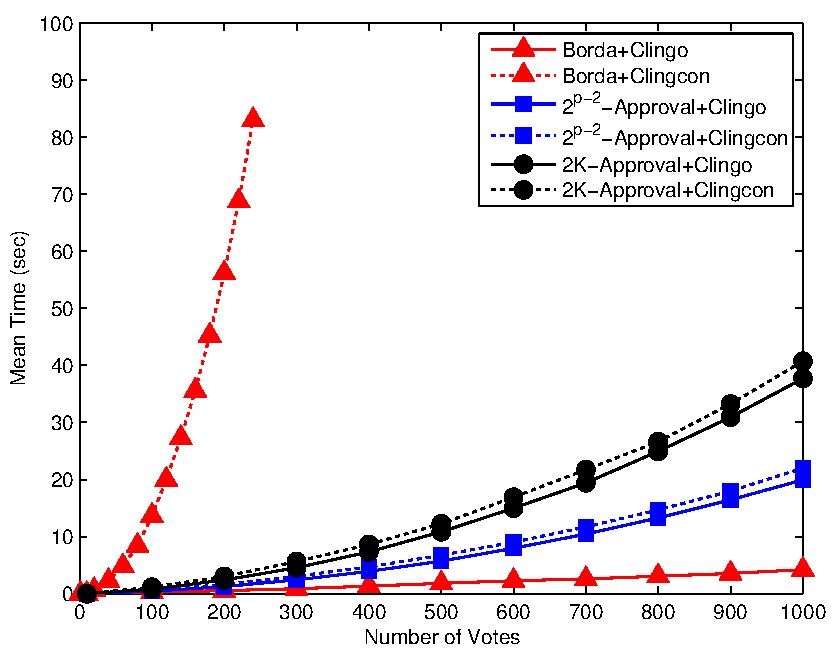
\includegraphics[width=\textwidth]{figs/figs_in_ADT/fixedIssues10SCICP.pdf}
%%		\caption{Winner, fixed \#Issues (10)}
%%		\label{fig:comparison:1}
%%	\end{subfigure}
%%  \begin{subfigure}[b]{0.5\textwidth}
%%		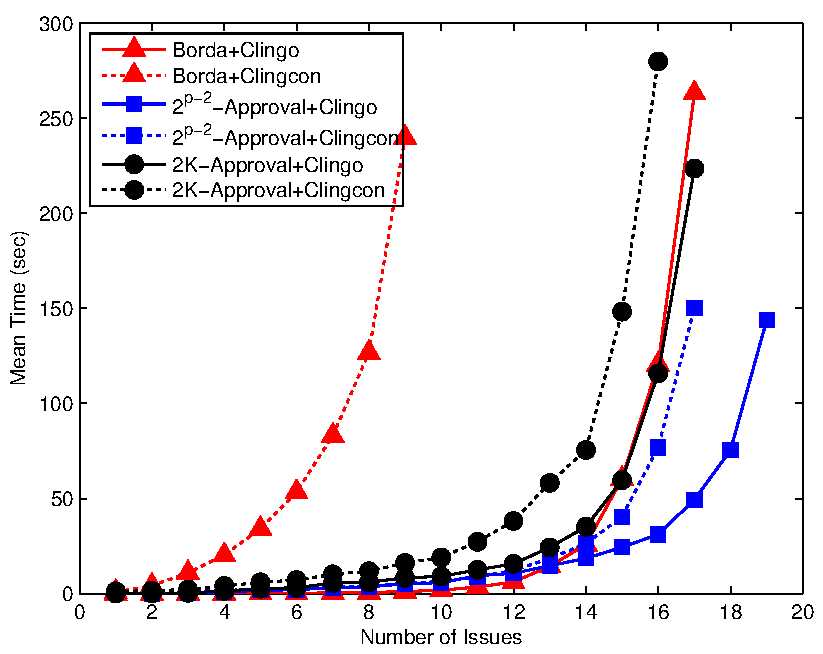
\includegraphics[width=\textwidth]{figs/figs_in_ADT/fixedVotes500SCICP.pdf}
%%    \caption{Winner, fixed \#Votes (500)}
%%		\label{fig:comparison:2}
%%	\end{subfigure}
%%  \\
%%  \begin{subfigure}[b]{0.5\textwidth}
%%		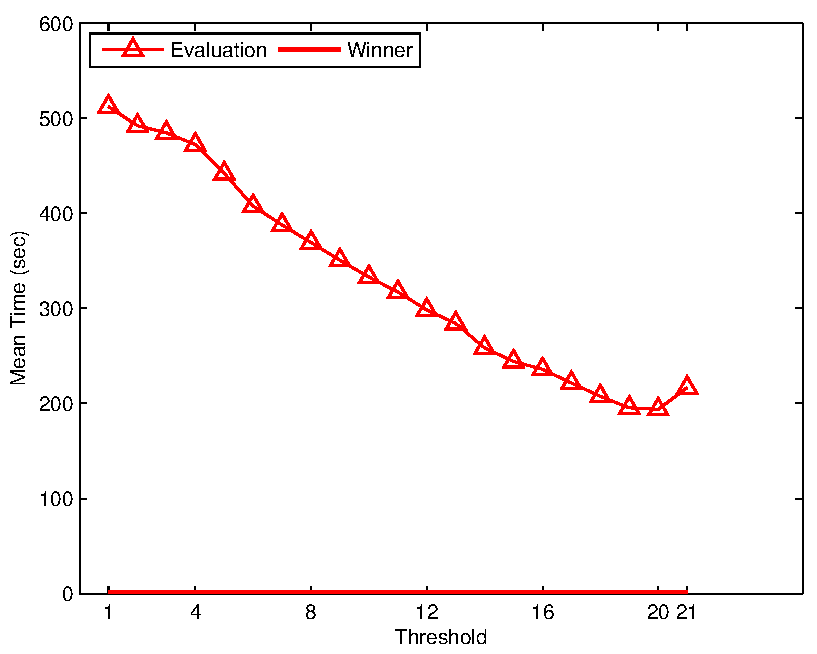
\includegraphics[width=\textwidth]{figs/figs_in_ADT/bordaClingo.pdf}
%%    \caption{Borda, \emph{clingo} (500votes/3attributes)}
%%		\label{fig:comparison:3}
%%	\end{subfigure}
%%  \begin{subfigure}[b]{0.5\textwidth}
%%		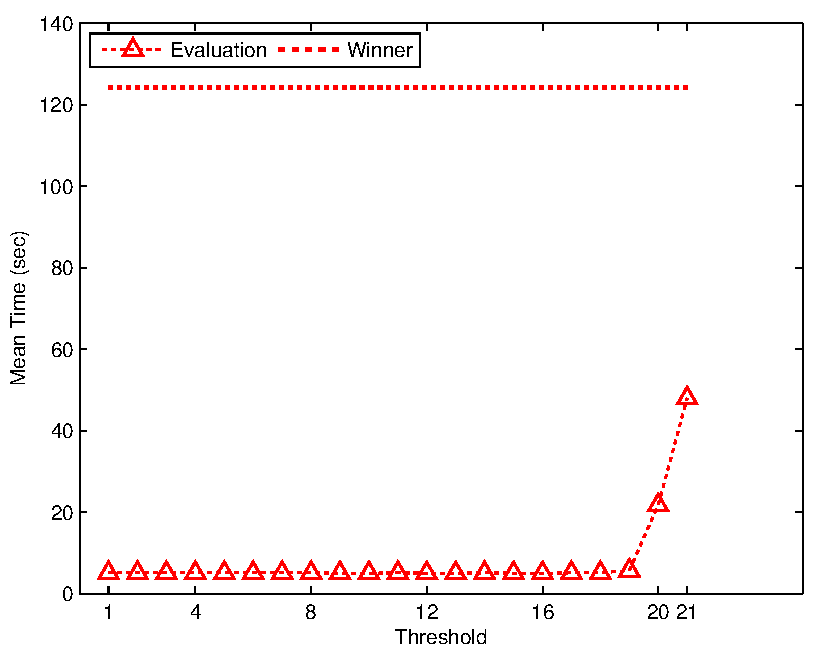
\includegraphics[width=\textwidth]{figs/figs_in_ADT/bordaClingcon.pdf}
%%    \caption{Borda, \emph{clingcon} (500votes/8attributes)}
%%		\label{fig:comparison:4}
%%	\end{subfigure}
%%  \\
%%  \begin{subfigure}[b]{0.5\textwidth}
%%		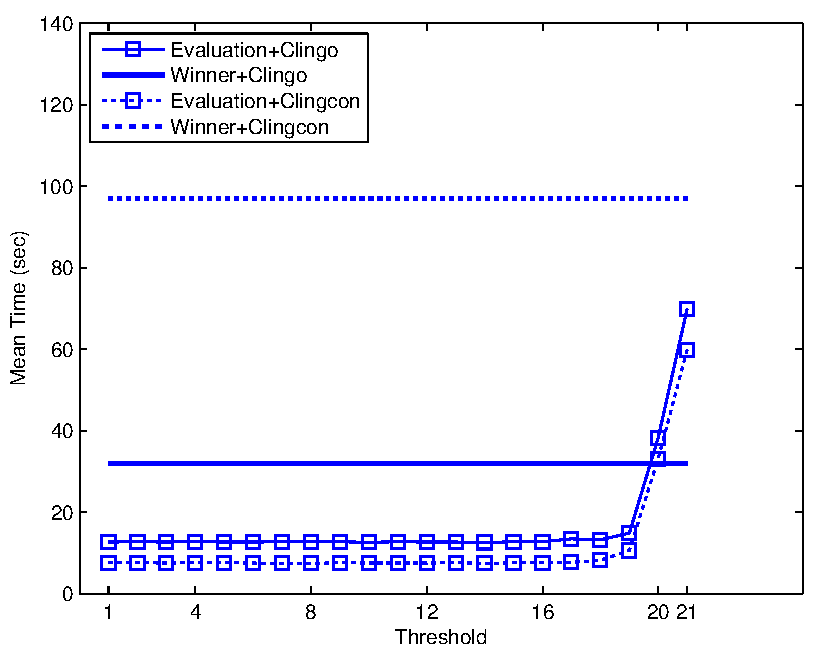
\includegraphics[width=\textwidth]{figs/figs_in_ADT/expAppSCICP.pdf}
%%    \caption{$2^{p-2}$-Approval (500votes/16attributes)}
%%		\label{fig:comparison:5}
%%	\end{subfigure}
%%  \begin{subfigure}[b]{0.5\textwidth}
%%		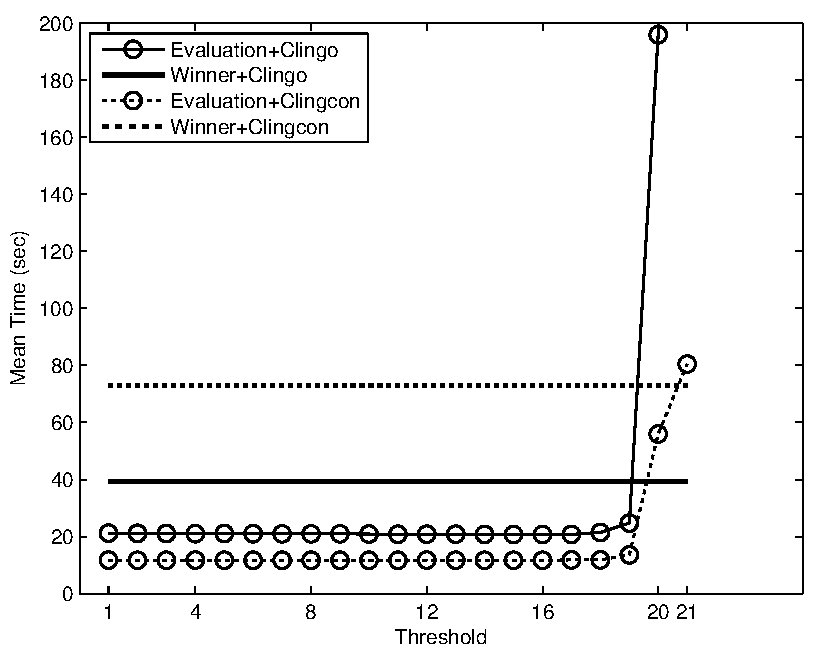
\includegraphics[width=\textwidth]{figs/figs_in_ADT/2kAppSCICP.pdf}
%%    \caption{$2K$-Approval (500votes/14attributes)}
%%		\label{fig:comparison:6}
%%	\end{subfigure}
%%	\end{tabular}
%%  \caption{Aggregating \textit{simple} LP-trees}
%%  \label{fig:comparison}
%%
%%\end{figure*}
%%
%%All our experiments were performed on a machine with an 
%%Intel(R) Core(TM) i7 CPU @ 2.67GHz and 8 GB RAM running 
%%Ubuntu 12.04 LTS.  
%%Each test case (using \emph{clingo 3.0.5} or \emph{clingcon 2.0.3}) was performed with 
%%a limit of 10 minutes.
%%
%%We first consider the winner problem. In the study, we consider the 
%%computation time with a fixed number of attributes (5/10/20) and for each number of attributes we range 
%%the number of votes in a profile up to 1000 for $\{Borda, 2^{p-2}$-$approval, 
%%2K$-$approval\} \times \{clingcon, clingo\}$.  
%%Then we fix the number of votes (500) and vary the number of attributes up to 20, again for 
%%same set of settings.  Each time 
%%result in seconds 
%%is computed as the mean of 10 tests over different randomly generated profiles of 
%%\textit{simple} LP-trees.
%%
%%For the evaluation problem, we compare its experimental complexity with that of the winner problem.
%%For each of the 10 randomly generated profiles, we compute the winning score 
%%$\WS$ 
%%and set the threshold for the evaluation problem with a percentage of $\WS$, starting with 
%%$5\%$ and incremented by $5\%$ for the following tests until we reach the full
%%value of $\WS$. We run one more test with the threshold $\WS+1$ (there is 
%%no solution then and the overall method allows for the experimental 
%%comparison of the hardness of the winner and evaluation problems).
%%That allows us to study the effectiveness of the maximization construct in
%%\emph{clingo} (the main difference between the \emph{winner} and the 
%%\emph{evaluation} problems is in the use of that construct in the 
%%encoding of the former).
%%We again present and compare average time results.
%%
%%\subsubsection{Varying the number of attributes and the number of votes}
%%%$p$ and $n$}
%%Our experiments on the winner problem for the three voting rules with 
%%the fixed number of attributes are consistent with the property that the problem
%%is solvable in polynomial time. 
%%Both \emph{clingo} and \emph{clingcon} scale up well.
%%\figref{comparison:1} depicts the results for the cases with 
%%10 attributes. When we fix the number of votes and vary the number of 
%%attributes the time grows exponentially with $p$ (cf. \figref{comparison:2}),
%%again consistently with the computational complexity of the problems
%%(NP-hardness).
%%
%%Generally \emph{clingo} is better compared to \emph{clingcon} in solving 
%%the winner problem for the three scoring rules. We attribute that first 
%%to the use of the optimization construct in \emph{clingo}, which allows
%%us to keep the size of the ground propositional theory low, and second to 
%%the effective way in which optimization constructs are implemented in that 
%%system. Thus, in these examples, the main benefit of \emph{clingcon},
%%its ability to avoid grounding and preprocessing by ``farming out'' some of the solving job
%%to a dedicated constraint solver, does not offer \emph{clingcon} the edge.
%%Finally, for both \emph{clingo} and \emph{clingcon}, Borda is the hardest
%%rule to deal with, especially when the number of attributes is large.
%%
%%\subsubsection{Comparison of the problems: evaluation vs winner}
%%
%%The evaluation problem can be reduced to the winner problem, as
%%an evaluation problem instance has an answer \textit{YES}
%%if and only if the score of the winner equals or exceeds the threshold.
%%Thus, the evaluation problem is at most as complex as
%%the winner problem.
%%
%%We compared the two problems by first solving the winner problem, and then
%%solving the evaluation problem on the same instances with the value of
%%the threshold growing at the step of 5\% of the winner score. That gives us
%%20 normalized points for each instance. In the last run (point 21 on the
%%$x$-axis) we used the winner's score plus 1 as the threshold to determine
%%the optimality of the winner's score. These experiments allow us to compare
%%the hardness of the winner problem (more precisely, the effectiveness 
%%of solvers) with that of the evaluation problem. 
%%
%%First, we note that for \emph{clingo}, the evaluation problem is
%%harder than the winner problem in the entire range for Borda ( 
%%\figref{comparison:3}), and for the two other rules, when the threshold 
%%is close to the winner's score or exceeds it (\figref{comparison:5}
%%and \figref{comparison:6}). We attribute that to the fact that the encodings 
%%of the evaluation problem have to model the threshold constraint with the 
%%\textit{\#sum} rule which, in \emph{clingo}, leads to large ground theories 
%%that it finds hard to handle. In the winner problem encodings, the \textit{\#sum} 
%%rule is replaced with an optimization construct, which allows us to keep
%%the size of the ground theory low.
%%
%%For \emph{clingcon} the situation is different. 
%%\figref{comparison:4}, \figref{comparison:5} and \figref{comparison:6}
%%show that the evaluation problem is easier than the winner problem
%%when the threshold values are smaller than the winning score and 
%%the evaluation problem becomes harder when the thresholds are close to it.
%%It seems to suggest that the constraint solver used by \emph{clingcon} 
%%performs well in comparison with the implementation of the optimization 
%%constructs in \emph{clingcon}.
%%Finally, in all cases \emph{clingcon} outperforms \emph{clingo} on the
%%evaluation problems. It is especially clear for Borda, where the range of
%%scores is much larger than in the case of approval rules. That poses a
%%challenge for \emph{clingo} that instantiates the \textit{\#sum} rule over
%%that large range, which \emph{clingcon} is able to avoid.

\section{Experiments}
Here we present and analyze the experimental results from solving the Winner problem
and the Evaluation problem using two Answer Set Programming solvers
$\clingo$ (version 4.2.1) and $\clingcon$ (version 2.0.3)
and one Constraint Satisfaction Problem solver $\toulbar$ (version 0.9.6.0-dev).

All our experiments were performed on a machine with an 
Intel(R) Core(TM) i7 CPU @ 2.67GHz and 8 GB RAM running 
Ubuntu 12.04 LTS.  

We first consider the winner problem. In the study, we consider the 
computation time with a fixed number of attributes (5/10/20) and for each number of attributes we range 
the number of votes in a profile up to 3000 for $\{Borda, 2^{p-2}$-$approval, 
2K$-$approval\} \times \{\clingcon, \clingo, \toulbar\}$.  
Then we fix the number of votes (1000) and vary the number of attributes up to 20, again for 
same set of settings.  Each time 
result in seconds 
is computed as the mean of 20 tests over different randomly generated profiles of 
LP-trees.

\subsection{Structure of the Simple LP Trees}
To experiment with the programs presented above and with \emph{clingo} and
\emph{clingcon} solvers, we generate logic programs that represent 
random LP-trees and profiles of random
LP-trees.
Our algorithm generates encodings of trees from the most general class CI-CP 
under the following restrictions:
(1) Each LP-tree has exactly two paths with the splitting node appearing 
at depth $d_s=\left \lfloor \frac{p}{2} \right \rfloor$;
(2) Each non-root node at depth $\leq d_s+1$ has exactly one parent;
(3) Each 
node at depth $> d_s+1$ has exactly two parents, one of which 
is at depth $< d_s$.\footnote{
The restrictions are motivated by the size of the representation
considerations. They ensure that the size of generated LP-trees is 
linear in the number of attributes.}

The algorithm starts by randomly selecting attributes to label the nodes on 
the path from the root to the splitting node and then, similarly, labels 
the nodes on each of the two paths (different labeling can be produced
for each of them). Then, for each non-root node, the algorithm selects at random
one or two parent nodes (as appropriate based on the location of the node).
Finally, the algorithm decides 
local preferences (for each combination of values of the parent attributes)
randomly picking one over the other. In each step, all 
possible choices are equally likely. We call CI-CP LP-trees satisfying 
these restrictions \emph{simple}. Each simple LP-tree has size 
linear in $p$.  \figref{MSCICP_tree} depicts a CI-CP tree of 
4 attributes in this class. 
\begin{figure}
\centering
	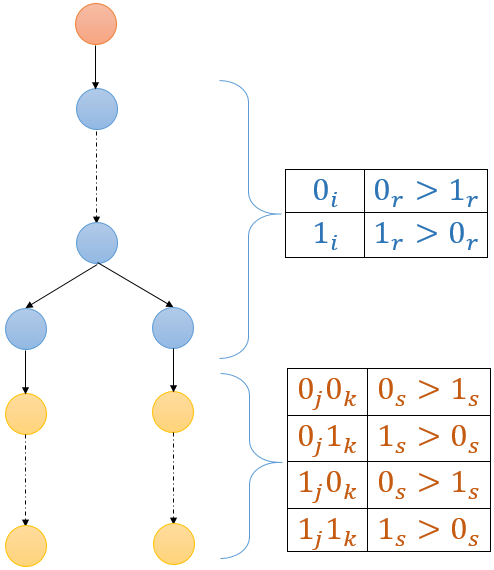
\includegraphics[width=0.5\textwidth]{img/simple_LP_tree.png}
\caption{\emph{Simple} CI-CP tree}
\label{fig:MSCICP_tree}
\end{figure}



\subsection{Solving the Winner Problem}

We refer to \ref{fig:win} for the empirical results on solving the Winner problem.  
Each point in a figure represents
an average of computation time spent on solving 20 different 
Winner problem instances given randomly
generated LP profiles.

\begin{figure*}[ht!]
	\centering
	\setlength{\tabcolsep}{0mm}
	\begin{tabular}{c}
  \begin{subfigure}[b]{0.44\textwidth}
		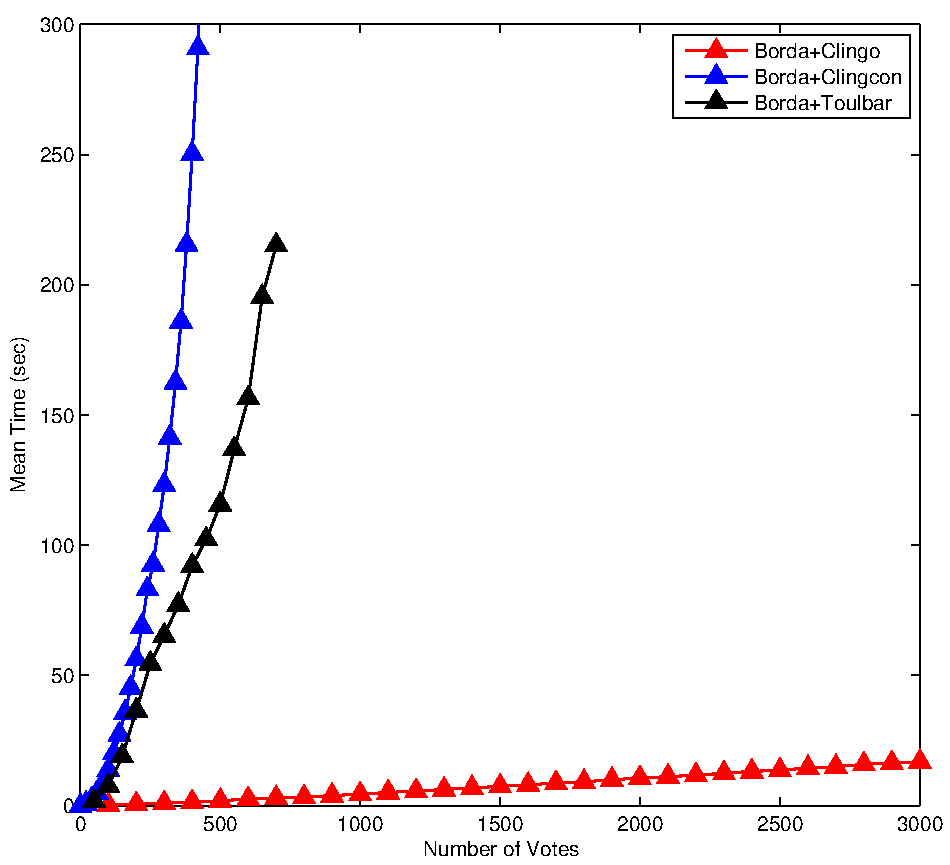
\includegraphics[width=\textwidth]{figs/bordaFIMSCICP.pdf}
		\captionsetup{font=scriptsize}
		\caption{Borda, fixed \#attributes(10)}
		\label{fig:comparison:win:1}
	\end{subfigure}
  \begin{subfigure}[b]{0.44\textwidth}
		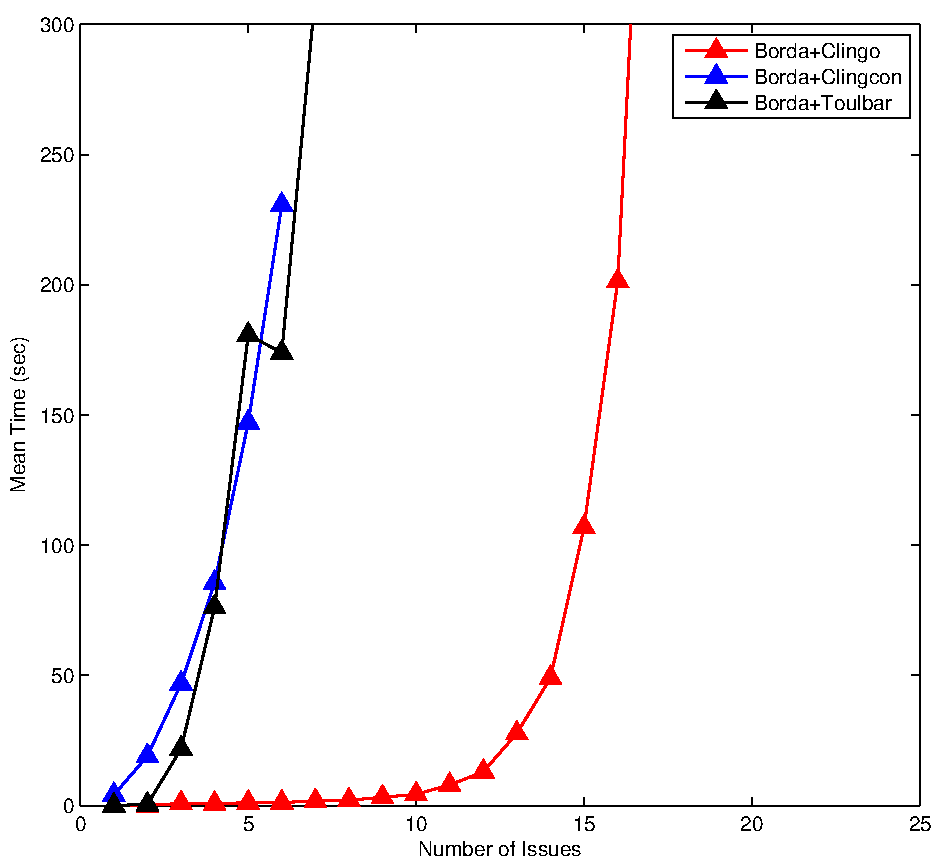
\includegraphics[width=\textwidth]{figs/bordaFVMSCICP.pdf}
		\captionsetup{font=scriptsize}
    \caption{Borda, fixed \#votes(1000)}
		\label{fig:comparison:win:2}
	\end{subfigure}
  \\
  \begin{subfigure}[b]{0.44\textwidth}
		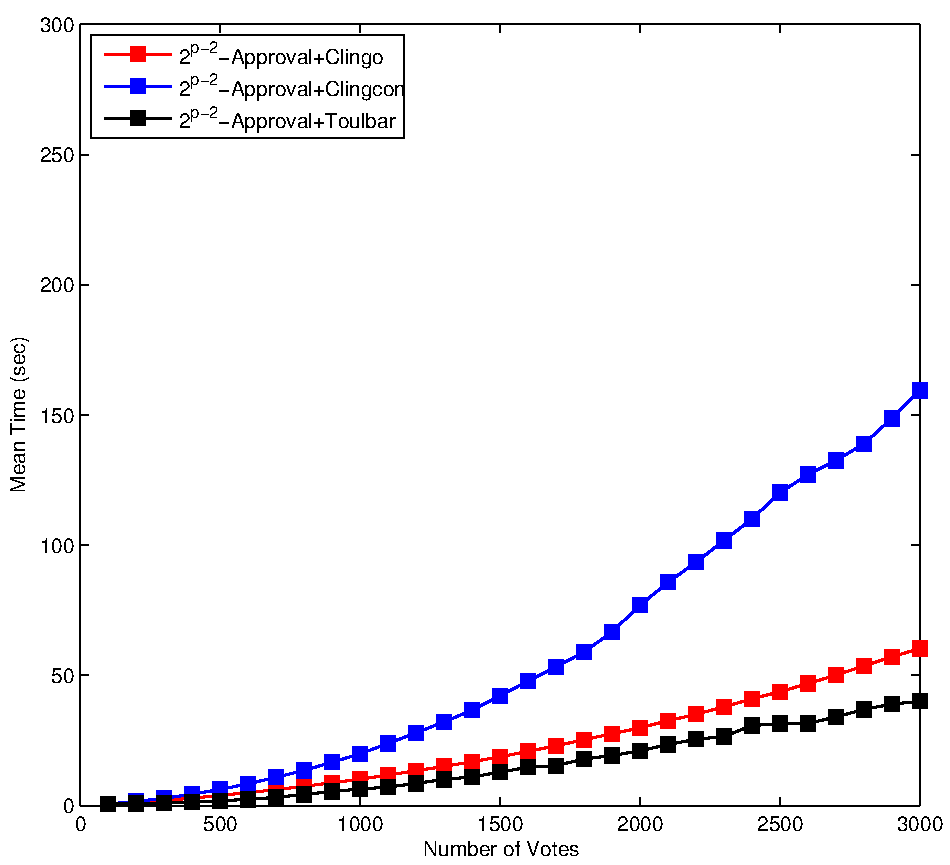
\includegraphics[width=\textwidth]{figs/expAppFIMSCICP.pdf}
		\captionsetup{font=scriptsize}
    \caption{$2^{p-2}$-Approval, fixed \#attributes(10)}
		\label{fig:comparison:win:3}
	\end{subfigure}
  \begin{subfigure}[b]{0.44\textwidth}
		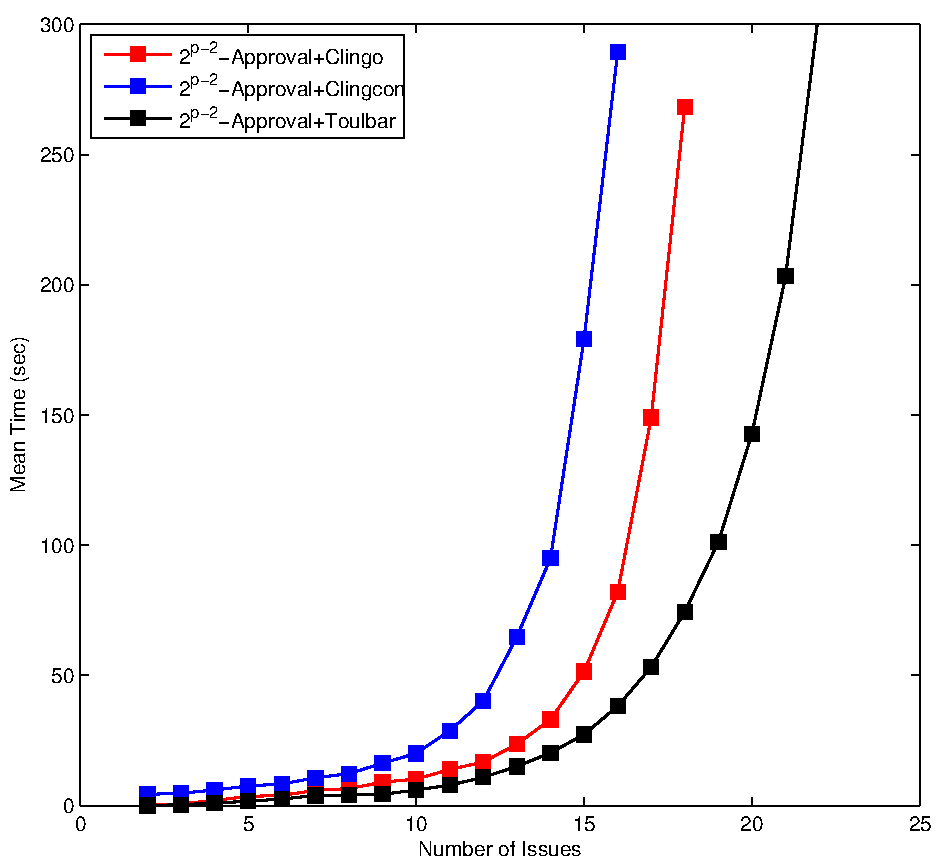
\includegraphics[width=\textwidth]{figs/expAppFVMSCICP.pdf}
		\captionsetup{font=scriptsize}
    \caption{$2^{p-2}$-Approval, fixed \#votes(1000)}
		\label{fig:comparison:win:4}
	\end{subfigure}
  \\
  \begin{subfigure}[b]{0.44\textwidth}
		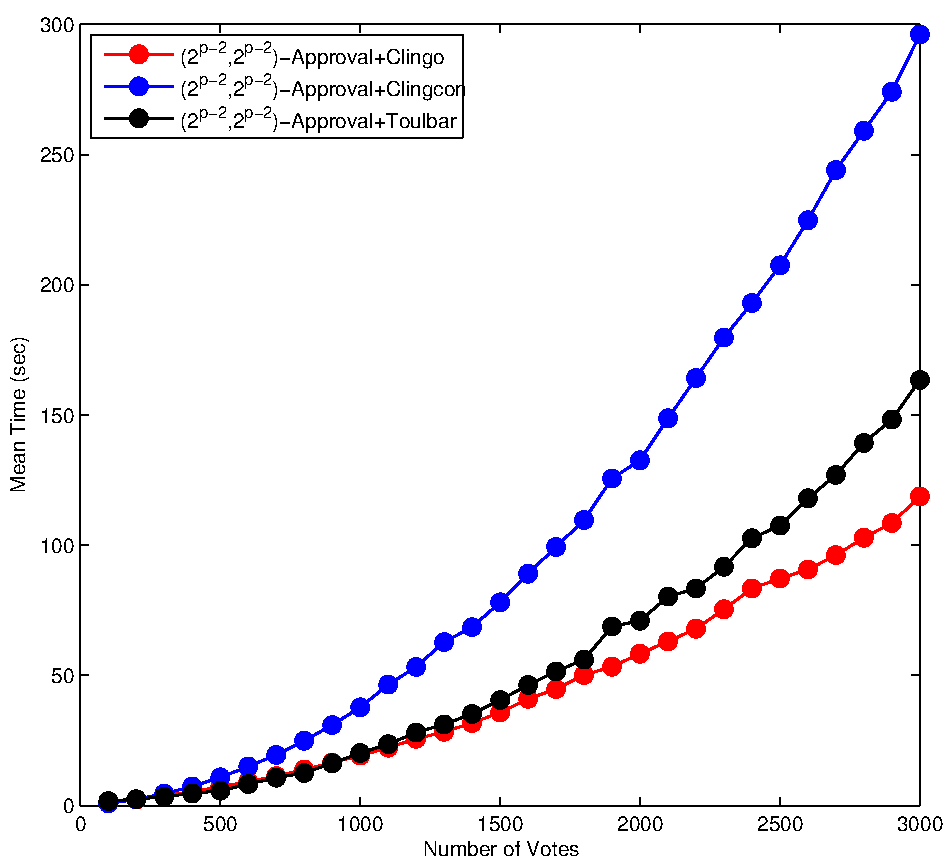
\includegraphics[width=\textwidth]{figs/2kAppFIMSCICP.pdf}
		\captionsetup{font=scriptsize}
    \caption{$2K$-Approval, fixed \#attributes(10)}
		\label{fig:comparison:win:5}
	\end{subfigure}
  \begin{subfigure}[b]{0.44\textwidth}
		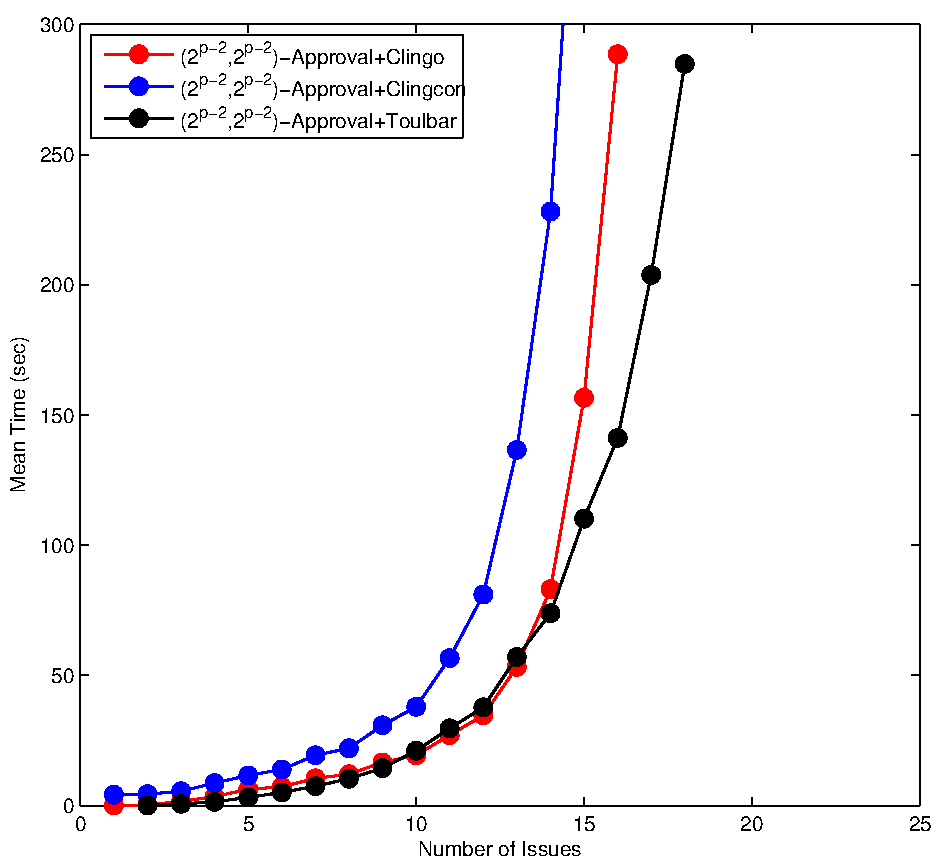
\includegraphics[width=\textwidth]{figs/2kAppFVMSCICP.pdf}
		\captionsetup{font=scriptsize}
    \caption{$2K$-Approval, fixed \#votes(1000)}
		\label{fig:comparison:win:6}
	\end{subfigure}
	\end{tabular}
  \caption{Solving the winner problem given \textit{simple} LP-trees}
  \label{fig:win}

\end{figure*}


It is clear that our experiments on the winner problem for the three voting rules with 
fixed number of attributes are consistent with the property that the problem
is solvable in polynomial time. All three solvers scale up well.
Figures \ref{fig:win}(a),(c) and (e) depict the result for the cases with 10 attributes.
When we fix the number of votes and vary the number of 
attributes the time grows exponentially with $p$ (cf. Figures \ref{fig:win}(b),(d) and (f)),
again consistently with the computational complexity of the problems (NP-hardness).

Generally $\clingo$ is better compared to $\clingcon$ in solving 
the winner problem for the three scoring rules. Moreover,
$\clingo$ outperforms $\toulbar$ in solving the winner problem for
the Borda rule, while $\toulbar$ performs better than $\clingo$
for the two approval rules.

For the winner problems, our experiments demonstrates that profiles
of LP-trees of practical sizes can be effectively handled by our
solvers, up to 3000 votes per profile over up to 20 attributes.
But going beyond 20 attributes remains a challenge.


%%\begin{figure*}[!ht]
%%	\centering
%%	\subfigure[Borda, fixed \#Issues (10)]{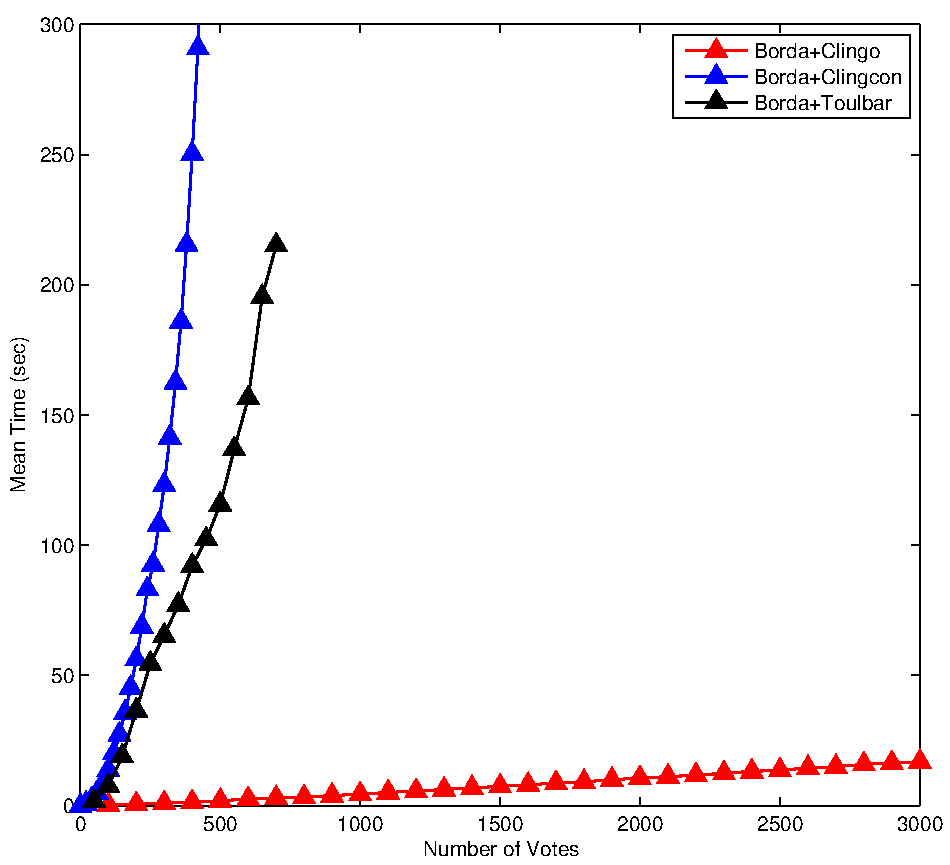
\includegraphics[width=0.45\textwidth]{figs/bordaFIMSCICP.pdf}}%
%%	\subfigure[Borda, fixed \#Votes (1000)]{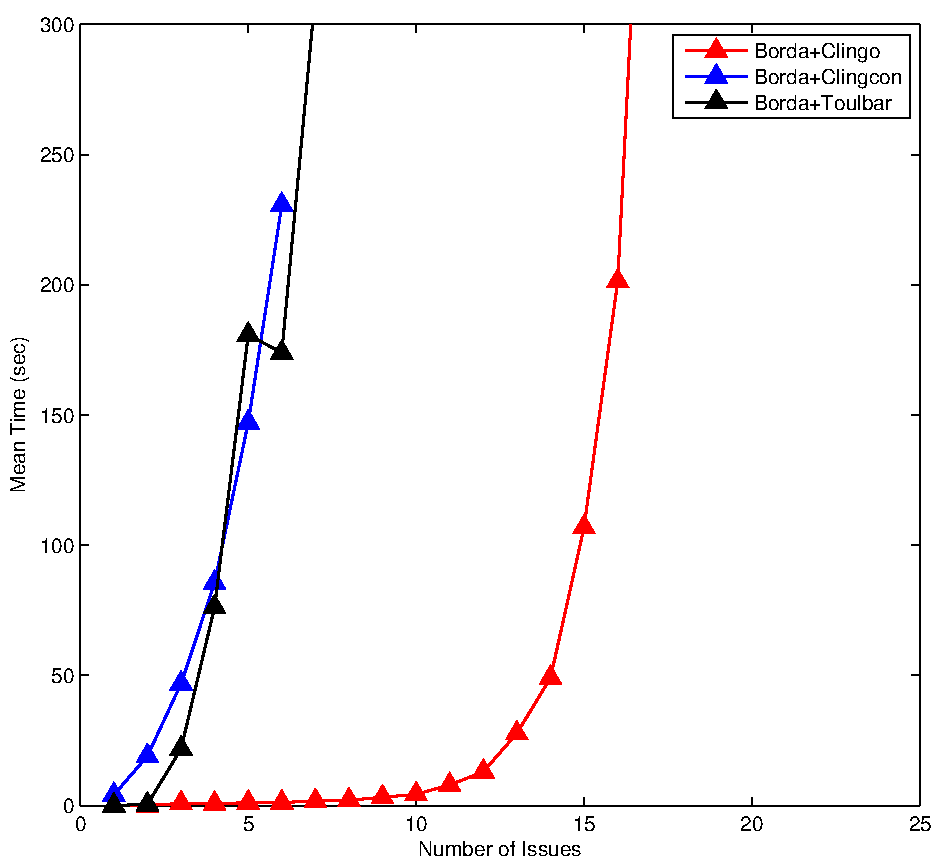
\includegraphics[width=0.45\textwidth]{figs/bordaFVMSCICP.pdf}} \\
%%	\subfigure[$2^{p-2}$-Approval, fixed \#Issues (10)]{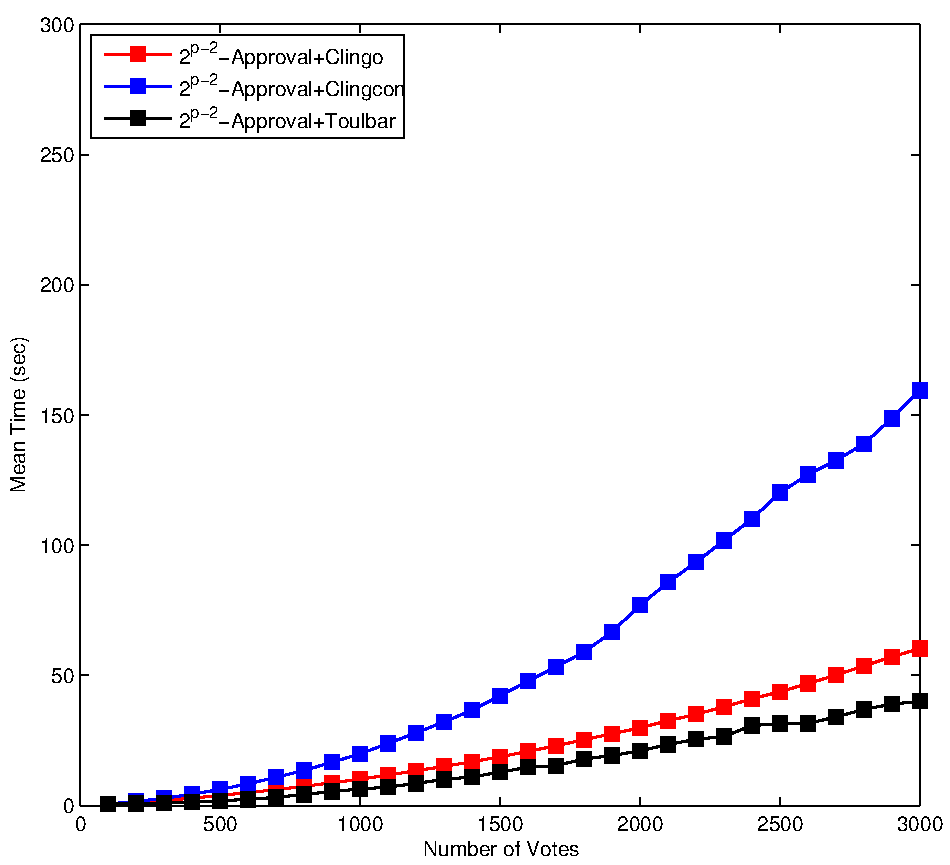
\includegraphics[width=0.45\textwidth]{figs/expAppFIMSCICP.pdf}}%
%%	\subfigure[$2^{p-2}$-Approval, fixed \#Votes (1000)]{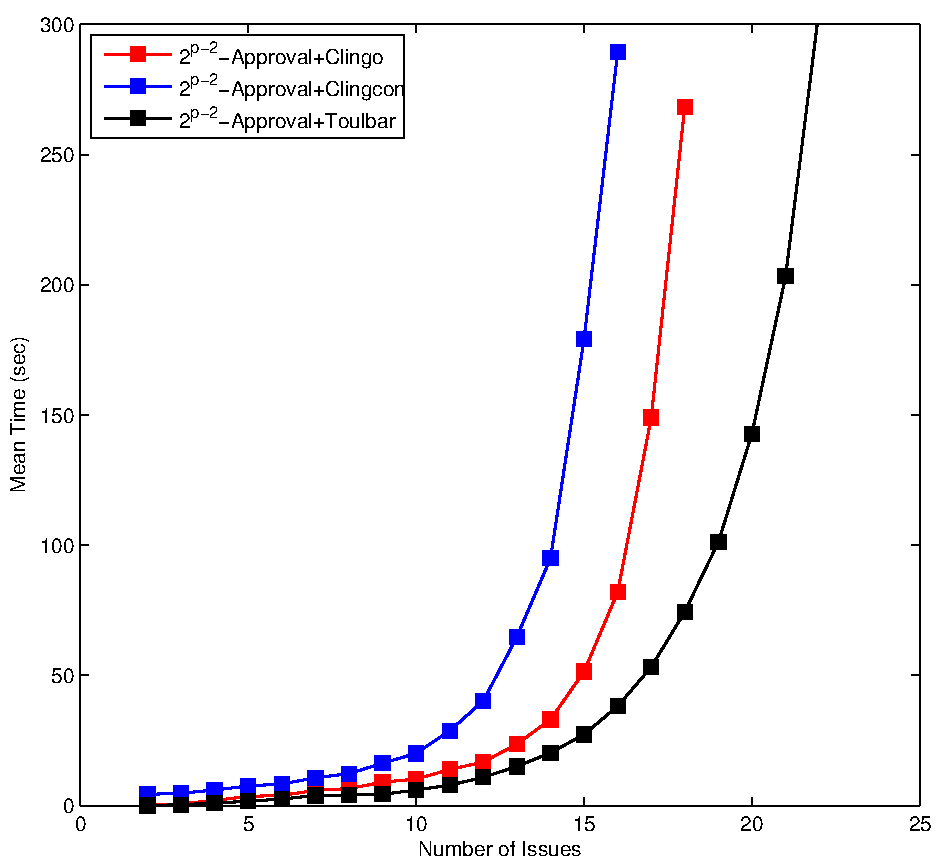
\includegraphics[width=0.45\textwidth]{figs/expAppFVMSCICP.pdf}} \\
%%	\subfigure[$2K$-Approval, fixed \#Issues (10)]{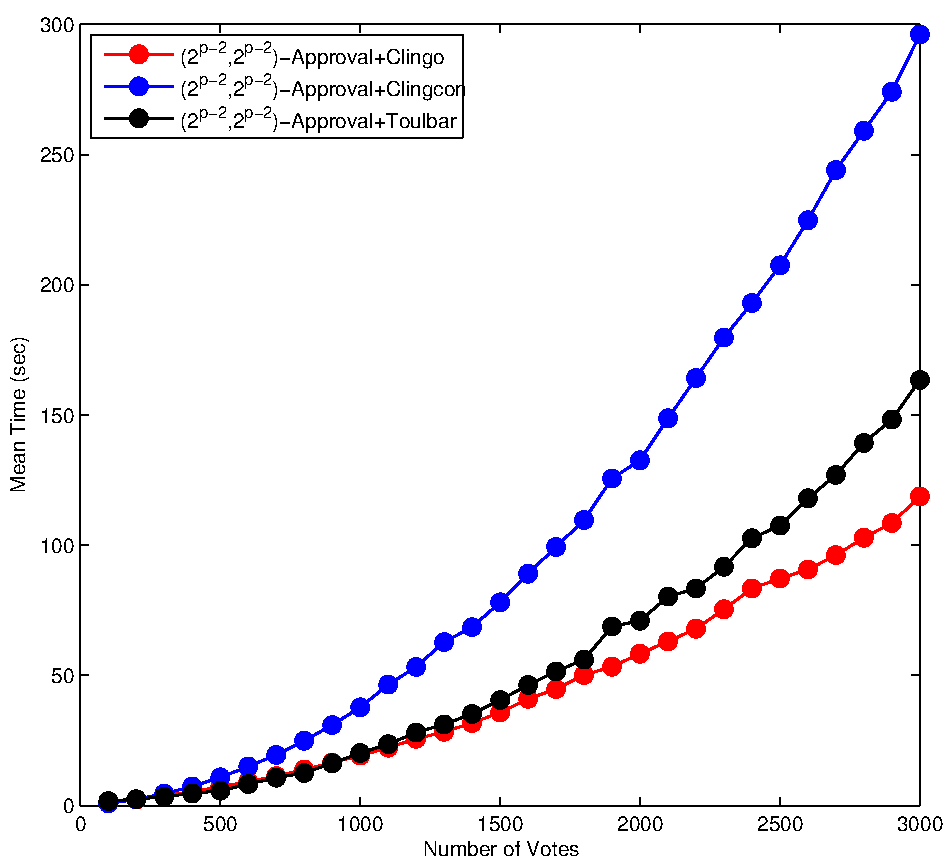
\includegraphics[width=0.45\textwidth]{figs/2kAppFIMSCICP.pdf}}%
%%	\subfigure[$2K$-Approval, fixed \#Votes (1000)]{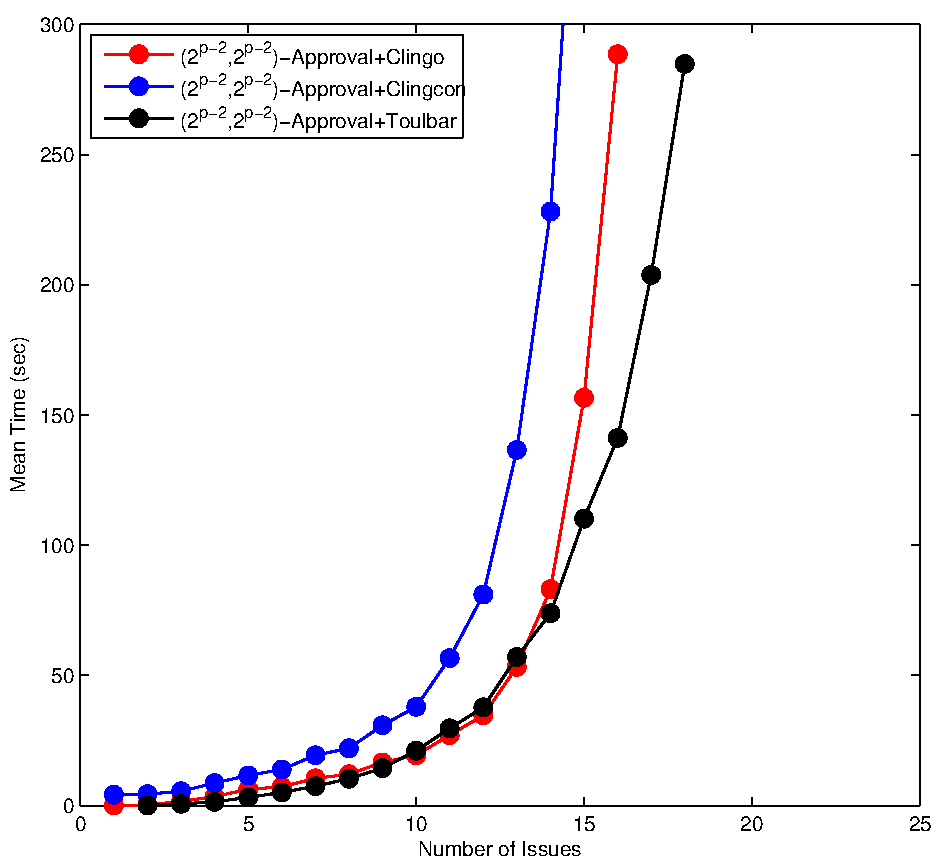
\includegraphics[width=0.45\textwidth]{figs/2kAppFVMSCICP.pdf}}
%%
%%  \caption{Solving the winner problem given \textit{simple} LP-trees}
%%  \label{fig:win}
%%
%%\end{figure*}



\subsection{Solving the Evaluation Problem}
The evaluation problem can be reduced to the winner problem, as
an evaluation problem instance has an answer \textit{YES}
if and only if the score of the winner equals or exceeds the threshold.
Thus, the evaluation problem is at most as complex as
the winner problem.

%%\begin{figure*}[!ht]
%%	\centering
%%	\subfigure[$2^{p-2}$-Approval (1000votes/13attributes)]{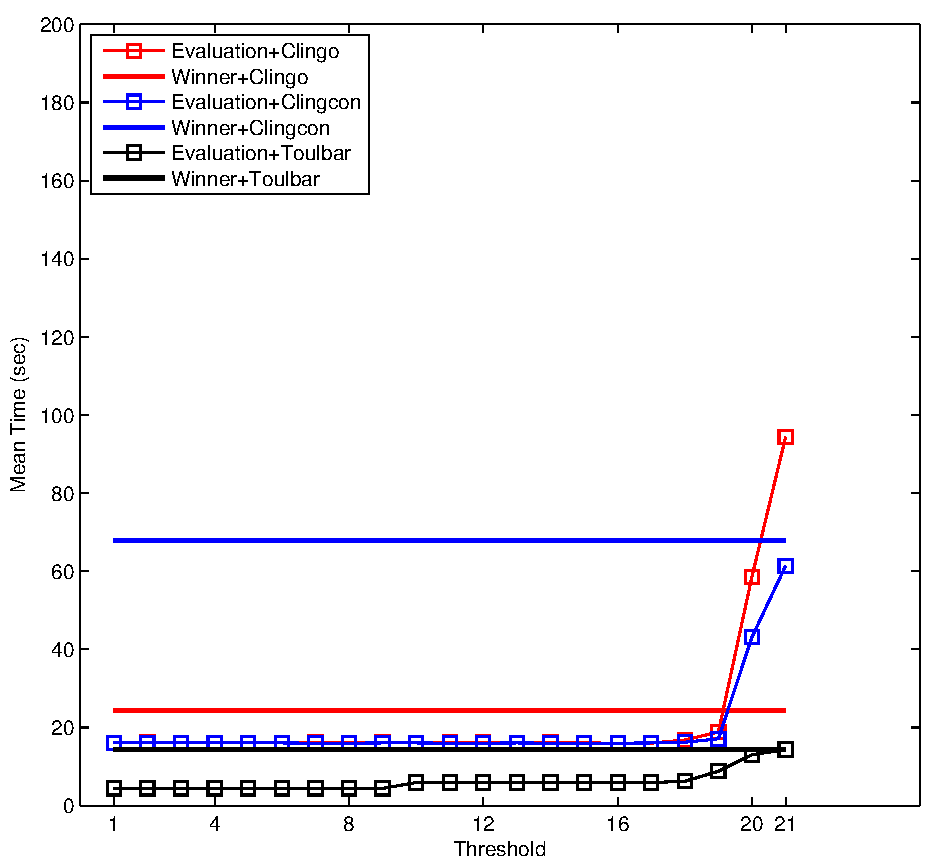
\includegraphics[width=0.45\textwidth]{figs/expAppMSCICP_1000v_13i.pdf}}%
%%	\subfigure[$2K$-Approval (1000votes/13attributes)]{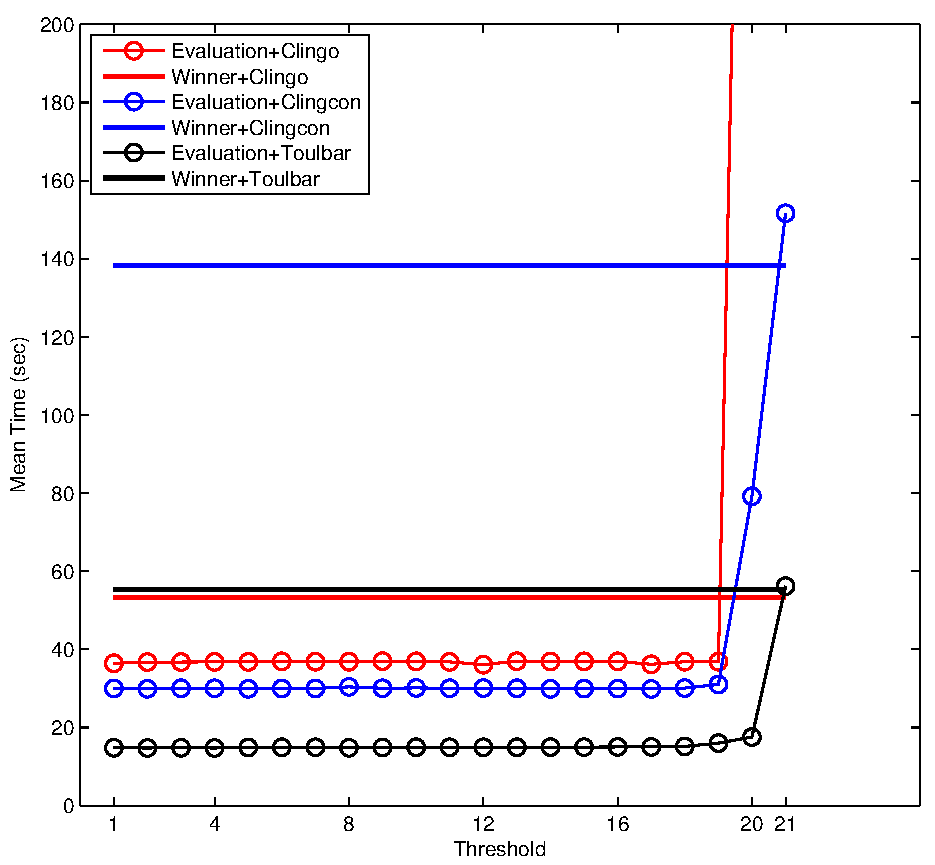
\includegraphics[width=0.45\textwidth]{figs/2kAppMSCICP_1000v_13i.pdf}}\\
%%	\subfigure[Borda (1000votes/4attributes)]{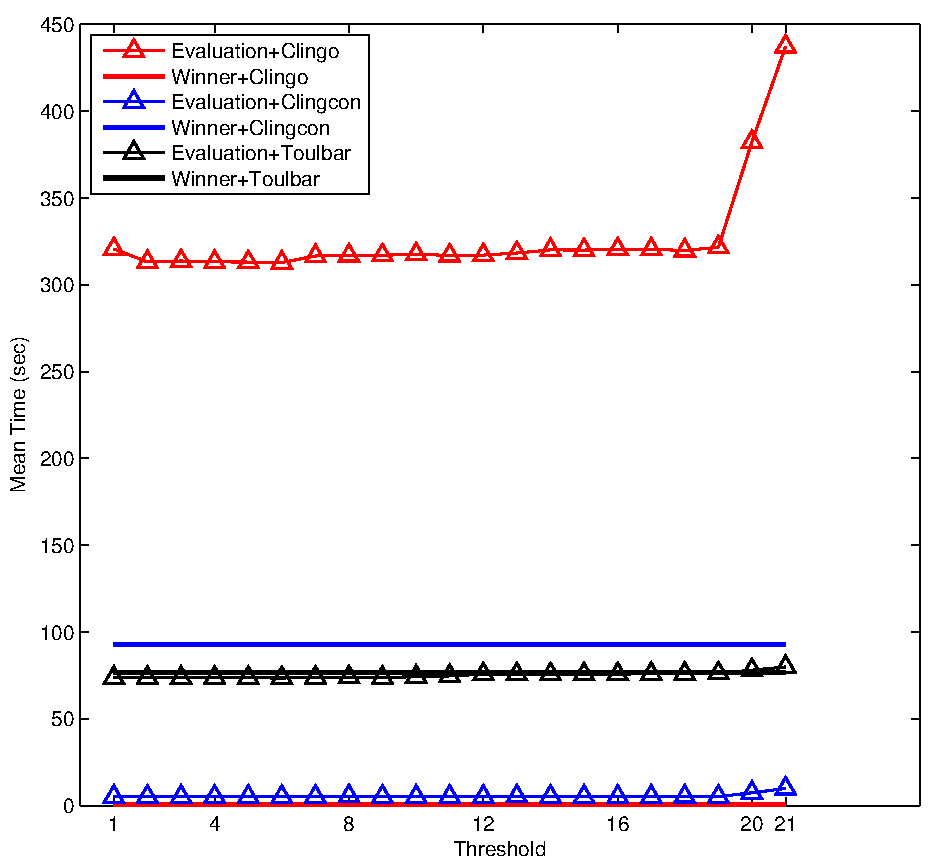
\includegraphics[width=0.45\textwidth]{figs/bordaMSCICP_1000v_4i.pdf}}
%%
%%  \caption{Solving the evaluation problem given \textit{simple} LP-trees}
%%  \label{fig:eval}
%%
%%\end{figure*}

\begin{figure*}[!ht]
	\centering
	\setlength{\tabcolsep}{0mm}
	\begin{tabular}{c}
  \begin{subfigure}[b]{0.5\textwidth}
		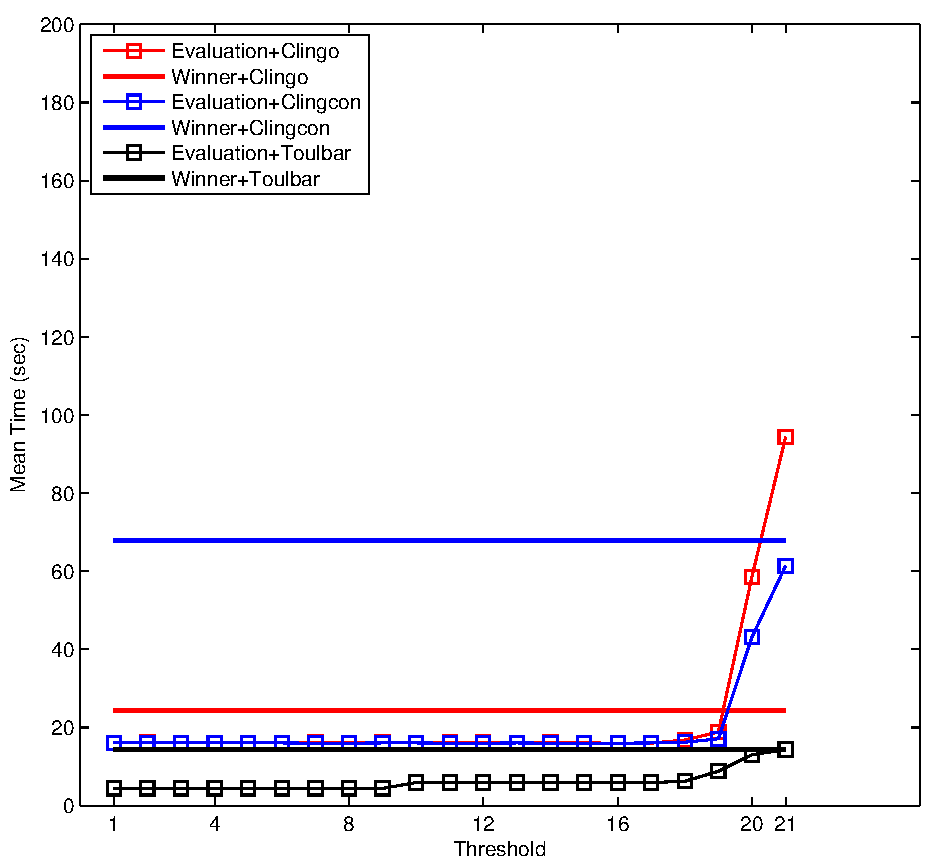
\includegraphics[width=\textwidth]{figs/expAppMSCICP_1000v_13i.pdf}
		\captionsetup{font=scriptsize}
		\caption{$2^{p-2}$-Approval (1000votes/13attributes)}
		\label{fig:comparison:eval:1}
	\end{subfigure}
  \begin{subfigure}[b]{0.5\textwidth}
		\includegraphics[width=\textwidth]{figs/2kAppMSCICP_1000v_13i.pdf}
		\captionsetup{font=scriptsize}
    \caption{$2K$-Approval (1000votes/13attributes)}
		\label{fig:comparison:eval:2}
	\end{subfigure}
  \\
  \begin{subfigure}[b]{0.5\textwidth}
		\includegraphics[width=\textwidth]{figs/bordaMSCICP_1000v_4i.pdf}
		\captionsetup{font=scriptsize}
    \caption{Borda (1000votes/4attributes)}
		\label{fig:comparison:eval:3}
	\end{subfigure}
	\end{tabular}
  \caption{Solving the evaluation problem given \textit{simple} LP-trees}
  \label{fig:eval}
\end{figure*}

For the evaluation problem, we compare its experimental complexity with
that of the winner problem. For each of the $20$ randomly generated profiles
of 1000 votes, we
compute the winning score $\WS$ and set the threshold for the evaluation problem
with a percentage of $\WS$, starting with $5\%$ and incremented by $5\%$ for the
following tests until we reach the full value of $\WS$. We run one more test with the
threshold $\WS +1$ (there is no solution then and the overall method allows for the
experimental comparison of the hardness of the winner and evaluation problems).
That allows us to study the effectiveness of solvers. We again present and
compare average time results.

First, we note that for $\clingo$, the evaluation problem is
harder than the winner problem in the entire range for Borda (\figref{eval}(c)).
We attribute that to the fact that the encodings 
of the evaluation problem have to model the threshold constraint with the 
\textit{\#sum} rule which, in $\clingo$, leads to large ground theories 
that it finds hard to handle. In the winner problem encodings, the \textit{\#sum} 
rule is replaced with an optimization construct, which allows us to keep
the size of the ground theory low.

Second, we notice that, except for Borda and $\clingo$,
the evaluation problem is easier than the winner problem
when the threshold values are smaller than the winning score and 
the evaluation problem becomes harder when the thresholds are close to it.
We refer to Figures \ref{fig:eval}(a), (b) and (c).

Thirdly, in all cases \emph{clingcon} outperforms \emph{clingo} on the
evaluation problems (cf. Figures \ref{fig:eval}(a), (b) and (c)). 
It is especially clear for Borda, where the range of
scores is much larger than in the case of approval rules. That poses a
challenge for \emph{clingo} that instantiates the \textit{\#sum} rule over
that large range, which \emph{clingcon} is able to avoid.

Finally, we compare the effectiveness of $\clingcon$ and $\toulbar$ on
solving the evaluation problems. Generally, $\clingcon$ performs better
for the Borda rule, whereas $\toulbar$ is better for the two approval rules.
Again, to see this, we refer to Figures \ref{fig:eval}(a), (b) and (c).


\section{Conclusions}
Aggregating votes expressed as LP-trees is a rich source of interesting
theoretical and practical problems. In particular, the complexity of the
winner and evaluation problems for scoring rules is far from
being fully understood. First results on the topic were provided by 
Lang et al. \cite{lang:aggLP}; our work exhibited another class of positional
scoring rules for which the problems are NP-hard and NP-complete, 
respectively. However, a full understanding of what makes a positional 
scoring rule hard remains an open problem.

Importantly, our results show that ASP tools are effective in modeling 
and solving the winners and the evaluation problems for some positional 
scoring rules such as Borda, $2^{p-2}$-approval and $2K$-approval. When 
the number of attributes is fixed the ASP tools scale up consistently with 
the polynomial time complexity. In general, the tools are practical even 
if the number of attributes is up to 15 and the number of votes is as high 
as 500. This is remarkable as 15 binary attributes determine the space of over 
30,000 alternatives. 

Finally, the preference aggregation problems form 
interesting benchmarks for ASP tools that stimulate advances in ASP
solver development. As the preference aggregation problems involve large 
domains, they put to the test those features of ASP tools that attempt 
to get around the problem of grounding programs over large domains. Our 
results show that the optimization statements in \emph{clingo} in 
general perform well. When they cannot be used, as in the evaluation 
problem, it is no longer the case. The solver \emph{clingcon}, which 
reduces grounding and preprocessing work by delegating some tasks to a constraint solver, 
performs well in comparison to \emph{clingo} on the evaluation problem,
especially for the Borda rule (and we conjecture, for all rules that
result in large score ranges).

In the future work we will expand our experimentation by developing
methods to generate richer classes of randomly generated LP-trees.
We will also consider the use of ASP tools to aggregate votes given in
other preference systems such as CP-nets \cite{bbdh03} and answer set 
optimization (ASO) preferences \cite{Brewka:ASO}.

%Note the copyright notice at the end of each chapter.
\copyrightnotice

%\chapter{Personalization in Multi-Modal Trip Planning\label{ch:trip}}
%\paragraph{\bf Abstract.}
In the setting of multi-modal trip planning, it is essential for
the planner to allow users to express personal constraints and preferences,
and to compute optimal trips accordingly.
In this work, we designed and implemented a personalizable multi-modal trip
planning framework.

\section{Personalizability}
Personalizability consists of two aspects: constraints and preferences.
From the viewpoint of the planner,
constraints, also referred to as hard constraints, are statements that the planner
has to satisfy during the planning process; whereas preferences, also called
soft constraints, are specifications that the planner will need to optimize.
We formulated constraints using linear temporal logic (LTL) and preferences as
a preferential cost function (PCF), and implemented our planner leveraging the
widely-used graph search algorithm the A*.

\subsection{Constraints}
\begin{itemize}
	\setlength\itemsep{1pt}
	\item Describe syntax and semantics of LTL in the setting of trip planning.
	\begin{itemize}
		\setlength\itemsep{0pt}
		\item Specifically, we need to point out the ``after" temporal connective,
					and we need to describe the semantics: what is a plan, why we can
					eliminate actions and put them as state attributes instead, etc.
	\end{itemize}
\end{itemize}
As constraints in the setting of trip planning are often declarative and
temporal, our choice of LTL is straightforward.
We now give a brief review of linear temporal logic (LTL).
Let $f$ be a propositional formula over a finite set $L$ of Boolean variables.  
LTL formulas are defined recursively as follows.
\begin{equation}
	\varphi = f | \varphi_1 \land \varphi_2 | \varphi_1 \lor \varphi_2 | \neg \varphi | 
		\bigcirc \varphi |	\Box \varphi | \Diamond \varphi | \varphi_1 \cA \varphi_2
\end{equation}
Note that we have $\varphi_1 \cA \varphi_2$, and it means that
``$\varphi_2$ holds right after $\varphi_1$ holds."

An intuitive constraint in trip planning could be ``I will never drive after biking or
taking the public transit."
In LTL, such constraint can be translated into an LTL formula
\begin{align*}
	((M=b) \lor (M=t)) \,\cA\, (\Box (\neg (M=c))).
\end{align*}

As the actions in trip planning is limited to taking different transportation modes,
in our definition of the semantics of LTL
these actions are subsumed into the interpretations of $L$, or \tit{states}.
The semantics of LTL is defined with regard to trajectories of states. 
Let $\sigma$ be a trajectory of states $S_0,a_1,S_1,\ldots,a_n,S_n$, and
$\sigma[i]$ a suffix $S_i, a_{i+1}, S_{i+1}, \ldots,a_n,S_n$.  We have
\begin{align*}
	\sigma \models f \;\; &\itiff \;\; S_0 \models f,\\
	\sigma \models \varphi_1 \land \varphi_2 \;\; &\itiff \;\; \sigma \models \varphi_1 \; and \; \sigma \models \varphi_2,\\
	\sigma \models \varphi_1 \lor \varphi_2 \;\; &\itiff \;\; \sigma \models \varphi_1 \; or \; \sigma \models \varphi_2,\\
	\sigma \models \neg \varphi \;\; &\itiff \;\; \sigma \not \models \varphi,\\
	\sigma \models \bigcirc \varphi \;\; &\itiff \;\; \sigma[1] \models \varphi,\\
	\sigma \models \Box \varphi \;\; &\itiff \;\; \forall 0 \leq i \leq n (\sigma[i] \models \varphi),\\
	\sigma \models \Diamond \varphi \;\; &\itiff \;\; \exists 0 \leq i \leq n (\sigma[i] \models \varphi),\\
	\sigma \models \varphi_1 \cA \varphi_2 \;\; &\itiff \;\; \forall 0 \leq i < n (\IF \; \sigma[i] \models \varphi_1, \sigma[i+1] \models \varphi_2).
\end{align*}


\subsection{Preferences}
\begin{itemize}
	\setlength\itemsep{1pt}
	\item Describe our preferential cost function (PCF).
	\begin{itemize}
		\setlength\itemsep{0pt}
		\item Describe why and how we break down time and money.
		\item Describe why and how we design coefficients to these time and money pieces.
		\item Describe why and how we design the two ratios: dollars per hour and dollars per aux.
	\end{itemize}
\end{itemize}

A state is described as a set of \tit{state variables}.
The state variables of a state $S$ include the transportation mode $M$ that led to $S$,
time spent $T$ so far per mode (e.g., $T_\bike$ for biking and $T_\public$ for
public transit), fare $D$ spent so far per mode (e.g., $D_\gas$ for driving and
$D_\taxi$ for taking a cab), and variables related to the auxiliary data once uploaded.
These extra data related variables are metrics such as the sum ($A_\SUM$),
the maximum ($A_\MAX)$, the minimum ($A_\MIN$), and the average ($A_\AVG$) data along the path.

We focused on weighted functions over state variables and
designed the cost function, called preferential cost function (PCF), that guides the
graph-based search engine in our trip planner as follows.
\begin{equation}
	\begin{aligned}
		\PCF(S) =& \beta_1 * (\alpha_1 \cdot T_\walk + \alpha_2 \cdot T_\wait + \ldots) \\
								&+ (D_\gas + D_\public + \ldots) \\
								&+ \beta_2 * (A_\SUM + \ldots),
	\end{aligned}
\end{equation}
where $\alpha_i$ are real numbers representing the relations among different time pieces,
and $\beta_1$ ($\beta_2$) is the ratio that essentially describes how much in dollars a user would pay to
save an hour (an auxiliary data, respectively).

\subsubsection{Preference Elicitation}
To gather these coefficients ($\alpha_i$ and $\beta_i$) in our $\PCF$, we designed interface to
elicit these numbers from the user.

\subsection{Reasoning with Constraints and Preferences}
\begin{itemize}
	\setlength\itemsep{1pt}
	\item Describe why and how we integrate constraints and preferences into A*.
\end{itemize}

We leveraged the widely-used A* search algorithm on top of our high-performance graph search
engine.  The A* algorithm incorporates the following cost function.
\begin{equation}
	f(S) = g(S) + h(S),
\end{equation}
where $g(S)$ is the cost of an optimal trip from the initial state to $S$, and
$h(S)$ is an admissible estimate of the cost of an optimal trip from $S$ to goal.

To prune the search space, we check satisfiability of the temporal constraints in LTL
at expansion of the search tree.
To guide the search engine, we set $g(S)=\PCF(S)$ and $h(S)$ the minimum estimate among
all available modes in $S$.

%%Note the copyright notice at the end of each chapter.
%\copyrightnotice

\chapter{Conclusion and Future Work\label{ch:summary}}
%I now discuss my ongoing research work, as well as point out directions of
%future research.
%My ongoing research work that, once done, would be included in 
%the final version of my dissertation contains the following components:
%
%\begin{enumerate}  \itemsep -4pt
%	\item Preference learning and approximation:
%		\begin{itemize} \itemsep -5pt
%			\item Learning forests of lexicographic preference trees.
%			\item Approximating CP-nets using lexicographic preference trees.
%		\end{itemize}
%	\item Preference reasoning:
%		\begin{itemize} \itemsep -5pt
%			\item Aggregating partial lexicographic preference trees (PLP-trees).
%			\item Preference misrepresenting in elections where votes are LP-trees or PLP-trees.
%		\end{itemize}
%\end{enumerate}

The research in my thesis is about various aspects of preferences:
preference modeling, preference learning, and preference reasoning.
Preferences is a major research component studied
in artificial intelligence (AI) and decision theory, and is closely related to the 
social choice theory considered by economists and political scientists. 
In my thesis, I 
explore emerging connections between preferences in AI and social choice theory. 
Most of my research is on qualitative preference representations 
that extend and combine
existing formalisms such as  
lexicographic preference trees (LP-trees) \cite{booth:learningLP}, 
answer-set optimization theories (ASO-theories) \cite{Brewka:ASO}, 
possibilistic logic \cite{DuboisLP91}, and 
conditional preference networks (CP-nets) \cite{boutilier2004cp};
on learning problems that aim at discovering qualitative preference 
models and predictive preference information from practical data; and on
preference reasoning problems centered around qualitative preference optimization 
and aggregation methods.
Applications of my research include recommender systems, decision support tools,
multi-agent systems, and Internet trading and marketing platforms.

%Regarding future research directions, I will establish a research program of data-driven
%preference engineering, including data-driven preference learning, and preference
%reasoning and applications.
%
%For data-driven preference learning, I plan to study methods and algorithms below.
%\begin{enumerate}
%	\item Recommender Systems\cite{adomavicius2005toward}:
%		\begin{itemize}
%			\item Collaborative
%			\item Content-based
%			\item Hybrid
%		\end{itemize}
%	\item Machine Learning (fitting function):
%		\begin{itemize}
%			\item Supervised learning (e.g., decision trees, random forests)
%			\item Label ranking\cite{hullermeier2008label}
%		\end{itemize}
%	\item Model-based Learning (learning interpretable decision models):
%		\begin{itemize}
%			\item Preference Elicitation (Human-in-the-Loop)
%			\item Conditional Preference Networks, Preference Trees
%			\item Stochastic Models (e.g., Choquet integral\cite{tehrani2011choquistic}, 
%						TOPSIS-like models\cite{agarwal2014preference})
%		\end{itemize}
%\end{enumerate}
%
%For preference reasoning and applications, I propose to investigate both theoretic
%and practical problems in areas as follows.
%\begin{enumerate}
%	\item Social Choice and Welfare\cite{arrow2010handbook,Brandt:COMSOC}:
%		\begin{itemize}
%			\item Voting
%			\item Fair division
%			\item Strategy-proof Social Choice
%		\end{itemize}
%	\item Automated Planning and Scheduling\cite{son2006planning,bienvenu2011specifying,bast2015route}:
%		\begin{itemize}
%			\item Travel scheduling
%			\item Manufacturing
%			\item Traffic control
%		\end{itemize}
%\end{enumerate}
\section{Future Work}
My long-term research goal is to study computational problems related to preferences, and 
develop applications that help people or software agents make better decisions.
Particularly, I intend to embed theories and practices on preferences into areas including
data science, and automated planning and scheduling.

\smallskip \noindent \textbf{Data science \  } Discovering preference 
models from large data sets and reasoning about them 
can be of great value when decisions need to be customized for individual users.
For instance, e-Commerce companies want to make quality marketing decisions
on what customers would be interested in purchasing at a future time.
I propose to introduce contextual information and human-in-the-loop into existing learning methods
(e.g., collaborative filtering and content-based filtering used in recommender systems), 
in order to provide context-aware and user-centered predictions.
On the collective level, I mean to leverage social science methods (e.g., voting rules)
to combine individual models for joint decisions.
I plan to build preferential data sets and develop predictive systems, with collaborators
or sponsors from fields 
such as machine learning, computer vision, psychology, cognitive science, and behavioral science.

\smallskip \noindent \textbf{Automated planning and scheduling \  }
In planning and scheduling, constraints and preferences of agents may be more faceted than simply
``fastest" or ``cheapest."
I propose to design mathematical models allowing
intuitive representations of these individual accommodations. 
Furthermore, I intend to implement systems
that automate the acquisition of user constraints and preferences, 
and the computation of optimal plans or schedules 
based on these user-specific information.
This line of research potentially promotes collaboration with researchers of expertise in
travel scheduling, manufacturing, and traffic control.

%Note the copyright notice at the end of each chapter.
\copyrightnotice


%-----------------------------------------------
\backmatter
%put your bibliography/references here.  Appendices go here as well. 
\bibliographystyle{plain}
\bibliography{mybib}

\chapter{Vita}
\singlespacing
\hypersetup{
    colorlinks,%
    citecolor=black,%
    filecolor=black,%
    linkcolor=black,%
    urlcolor=black 
    %urlcolor=mygreylink     % can put red here to better visualize the links
}
\urlstyle{same}
\definecolor{mygrey}{gray}{.85}
\definecolor{mygreylink}{gray}{.40}
\textheight=9.0in
\raggedbottom
\raggedright
\setlength{\tabcolsep}{0in}

% Adjust margins
\addtolength{\oddsidemargin}{-0.375in}
\addtolength{\evensidemargin}{0.375in}
\addtolength{\textwidth}{0.5in}
\addtolength{\topmargin}{-.375in}
\addtolength{\textheight}{0.75in}

%-----------------------------------------------------------
%Custom commands
\newcommand{\resitem}[1]{\item #1 \vspace{-2pt}}
\newcommand{\resheading}[1]{{\large \colorbox{mygrey}{\begin{minipage}{\textwidth}{\textbf{#1 \vphantom{p\^{E}}}}\end{minipage}}}}
\newcommand{\ressubheading}[4]{
\begin{tabular*}{6.5in}{l@{\extracolsep{\fill}}r}
		\textbf{#1} & #2 \\
		\textit{#3} & \textit{#4} \\
\end{tabular*}\vspace{-6pt}}

\newcommand{\ressubsubheading}[2]{
\begin{tabular*}{6.5in}{l@{\extracolsep{\fill}}r}
		\textit{#1} & \textit{#2} \\
\end{tabular*}\vspace{-6pt}}
\renewcommand{\baselinestretch}{0.9}
%-----------------------------------------------------------

\newcommand{\mywebheader}{
\begin{tabular*}{6.5in}{l@{\extracolsep{\fill}}r}
	\textbf{\LARGE Xudong Liu} 
		%& \href{http://www.cs.uky.edu/~liu/}{http://www.cs.uky.edu/$\sim$liu/} $\bullet$ liu@cs.uky.edu\\
		& Born in Zaozhuang, Shandong, China.
	\end{tabular*}
\\
\vspace{0.1in}}

% CHANGE HEADER SOURCE HERE
\mywebheader

%%%%%%%%%%%%%%%%%%%%%%
%\resheading{Research Interests}
%%I am looking for a 2015 summer intern position in software development engineering.
%My research focuses on exciting topics in artificial intelligence and social science, including
%preferences (i.e., preference modeling, learning and reasoning), 
%data-driven and computational social science, 
%knowledge representation and reasoning, 
%decision theory, data mining, and machine learning.
%\vspace{3pt}

%%%%%%%%%%%%%%%%%%%%%%
\resheading{Education}
			\ressubheading{University of Kentucky}{USA}
			{Doctor of Philosophy, computer science
				}
			{Aug. 2010 -- present}\\  \vspace{6pt}
			{GPA:\textbf{4.00}/4.00 \\ Advisor: Dr. Miroslaw Truszczynski}  
				%\vspace{-6pt}
				%{ \small
				%\begin{itemize}
				%	%\resitem{\textbf{Available for internship: July 23, 2009; Graduation follows internship}}
				%	\resitem{\textbf{Courses}: 
				%			Modern Operating Systems, 
				%			Numerical Analysis, 
				%			Algorithm Design,
				%			Distributed Operating System, 
				%			Satisfiability and Equivalence Checking, 
				%			Database Systems, 
				%			Computer Networks, 
				%			Networks Security, 
				%			Preferences in AI and Decision Theory, 
				%			Principles of Constraint Satisfaction,
				%			Comparative Decision Making, 
				%			Preparing Future Faculty, and Grant Writing.}
				%\end{itemize}
				%}
%\begin{comment}
			\ressubheading{Harbin Institute of Technology}{China}
				{Bachelor of Engineering, software engineering}{Aug. 2006 -- July 2010}\\ \vspace{6pt}
				{GPA:3.56/4.00 \\ Advisor: Prof. Yushan Sun}
%\end{comment}
\vspace{3pt}


%%%%%%%%%%%%%%%%%%%%%%
\resheading{Employment}
			\ressubheading{{R\&D Intern}}{Palo Alto Research Center (PARC), USA}
			{Supervisor: Dr. Christian Fritz}
			{Jun. 2015 -- Aug. 2015}
			\vspace{6pt}
				%{ 
				%\begin{itemize}
				%	\resitem{Conducted research on and developed system modules for representing 
				%		and reasoning about user constraints and preferences in 
				%		trip planning.}
				%\end{itemize}
				%}
			\ressubheading{{Graduate Research Assistant}}{University of Kentucky, USA}
			{Advisor: Dr. Miroslaw Truszczynski}
			{Aug. 2010 -- May 2015}
			\vspace{6pt}
				%{
				%\begin{itemize}
				%	\resitem{Conducted research on logic-based knowledge representation formalisms, 
				%		studied and built
				%		tools for representing and reasoning about constraints and preferences in artificial intelligence.}
				%\end{itemize}
				%}
			\ressubheading{{Graduate Teaching Assistant}}{University of Kentucky, USA}
			{Advisors: Dr. Truszczynski, Dr. Pike and Dr. Moore}
			{Aug. 2010 -- May 2015}
			\vspace{6pt}
				%{
				%\begin{itemize}  \itemsep -2pt
				%	\resitem{CS215 - Introduction to Program Design and Problem Solving: leading lab
				%		sessions, grading assignments, preparing exam questions and solutions,
				%		and holding office hours.}
				%	\resitem{CS375 - Logic and Theory of Computing: grading assignments, 
				%		preparing assignment solutions,
				%		and holding office hours.}
				%	\resitem{CS463G - Introduction to Artificial Intelligence: guest instructor,
				%		on knowledge representation and reasoning, e.g., propositional logic, and
				%		first-order logic.}
				%\end{itemize}
				%}
			\ressubheading{{Undergraduate Teaching Assistant}}{Harbin Institute of Technology, China}
			{Advisor: Prof. Yushan Sun}
			{Aug. 2008 -- May 2010}
			\vspace{6pt}
				%{
				%\begin{itemize}  \itemsep -2pt
				%			\resitem{Compilers and J2EE, including
				%				leading lab sessions and grading assignments.}
				%\end{itemize}
				%}
			\ressubheading{{Undergraduate Intern}}{Information Security Lab, Harbin Institute of Technology, China}
			{Advisor: Prof. Yushan Sun}
			{Aug. 2009 -- May 2010}
				%{
				%\begin{itemize}  \itemsep -2pt
				%			\resitem{Used PHP, MySQL and Apache Tomcat to implement modules of a management system.}
				%\end{itemize}
				%}
\vspace{3pt}


%%%%%%%%%%%%%%%%%%%%%%%%%%%%%%%%%%%%%%%%%%%%%%%%%%%%%%
\resheading{Professional Services}
	\begin{description} \itemsep -3pt
		\item[Student member:] {AAAI}
		\item[Student volunteer:] {AAAI-15}
		\item[Program committee:] {IJCAI-16, IJCAI-13}
		\item[Paper reviewer:] {JAIR, AAAI-14, ISAIM-14}
		\item[Local arrangement committee:] {ADT-15, LPNMR-15, ICLP-11, NonMon@30-10}
	\end{description} % End Skills list
\vspace{3pt}



%%%%%%%%%%%%%%%%%%%%%%%%%%%%%%%%%%%%%%%%%%%%%%%%%%%%%%
\resheading{Refereed Publications}
\begin{enumerate}  \itemsep -3pt
	\item \textbf{Xudong Liu}.
		\textit{Modeling, Learning and Reasoning with Qualitative Preferences}.
		In Proceedings of the 4th International Conference on Algorithmic Decision Theory (ADT),
		volume 9346, pages 587-592, 2015. Springer
	\item \textbf{Xudong Liu} and Miroslaw Truszczynski.
		\textit{Reasoning with Preference Trees over Combinatorial Domains}.
		In Proceedings of the 4th International Conference on Algorithmic Decision Theory (ADT),
		volume 9346, pages 19-34, 2015. Springer
	\item \textbf{Xudong Liu} and Miroslaw Truszczynski.
		\textit{Learning Partial Lexicographic Preference Trees over Combinatorial Domains}.
		In Proceedings of the 29th AAAI Conference on Artificial Intelligence (AAAI),
		pages 1539-1545, 2015. AAAI Press
	\item \textbf{Xudong Liu} and Miroslaw Truszczynski.
		\textit{Preference Trees: A Language for Representing and Reasoning about Qualitative Preferences}.
		In Proceedings of the 8th AAAI Multidisciplinary Workshop on Advances in Preference 
		Handling (MPREF), pages 55-60, 2014. AAAI Press
	\item \textbf{Xudong Liu} and Miroslaw Truszczynski.
		\textit{Aggregating Conditionally Lexicographic Preferences Using Answer Set Programming Solvers}.
		In Proceedings of the 3rd International Conference on Algorithmic Decision Theory (ADT),
		volume 8176, pages 244-258, 2013. Springer
	\item Matthew Spradling, Judy Goldsmith, {\bf Xudong Liu}, Chandrima Dadi and Zhiyu Li.
		\textit{Roles and Teams Hedonic Game}.
		In Proceedings of the 3rd International Conference on Algorithmic Decision Theory (ADT), 
		volume 8176, pages 351-362, 2013. Springer
	\item {\bf Xudong Liu}. \textit{Aggregating Lexicographic Preference Trees Using Answer Set Programming: Extended Abstract}. 
In 23rd International Joint Conference on Artificial Intelligence Doctoral Consortium (IJCAI DC), 2013.
\end{enumerate}

\vspace{3pt}
%%%%%%%%%%%%%%%%%%%%%%%%%%%%%%%%%%%%%%%%%%%%%%%%%%%%%%

%\resheading{Technical Talks}
%
%\begin{enumerate}  \itemsep -3pt
%	\item \textit{Personalization in Trip Planning}. Oral.
%		At the Keeping Current Seminar, Department of Computer Science,
%		University of Kentucky, 2015.
%	\item \textit{Preference and Social Choice over Combinatorial Domains}. Oral. 
%		At the 1st ADT/LPNMR Doctoral Consortium (ADT/LPNMR-DC-15),
%		Lexington, Kentucky, USA, 2015.
%	\item \textit{Modeling, Learning and Reasoning with Qualitative Preferences}. Poster. 
%		At the 1st ADT/LPNMR Doctoral Consortium (ADT/LPNMR-DC-15),
%		Lexington, Kentucky, USA, 2015.
%	\item \textit{Reasoning with Preference Trees over Combinatorial Domains}. Oral.
%		At the 4th International Conference on Algorithmic Decision Theory (ADT-15),
%		Lexington, Kentucky, USA, 2015.
%	\item \textit{On Personalizability and Extensibility of Multi-Modal Trip Planning}. Oral.
%		At Dialog, Palo Alto Research Center, Palo Alto, California, USA, 2015.
%	\item \textit{Constraints and Preferences in Multi-modal Trip Planning}. Poster.
%		At the PARC Summer Intern Poster Session, Palo Alto Research Center, 
%		Palo Alto, California, USA, 2015.
%	\item \textit{Learning Partial Lexicographic Preference Trees over Combinatorial Domains}. 
%		Oral (ratio: 12\%=238/1991).
%		At the 29th AAAI Conference on Artificial Intelligence (AAAI-15), 
%		Austin, Texas, USA, 2015.
%	\item \textit{Preference Trees: A Language for Representing and Reasoning about Qualitative Preferences}. Oral.
%		At the 8th Multidisciplinary Workshop on Advances in Preference Handling (MPREF-14), 
%		Quebec City, Canada, 2014.
%	\item \textit{Aggregating Conditionally Lexicographic Preferences Using Answer Set Programming Solvers}. Oral.
%		At the 3rd International Conference on Algorithmic Decision Theory (ADT-13),
%		Universite lebre de Bruxelles, Belgium, 2013.
%	\item \textit{Reasoning About Lexicographic Preferences Over Combinatorial Domains}.
%		At the Keeping Current Seminar, Department of Computer Science, 
%		University of Kentucky, 2013.
%	\item \textit{Roles and Teams Hedonic Game}. Oral.
%		At the 7th Multidisciplinary Workshop on Advances in Preference Handling (MPREF-13),
%		Tsinghua University, Beijing, China, 2013.
%	\item \textit{Aggregating Conditionally Lexicographic Preferences Using Answer Set Programming Solvers}. Oral.
%		At the 7th Multidisciplinary Workshop on Advances in Preference Handling (MPREF-13),
%		Tsinghua University, Beijing, China, 2013.
%	\item \textit{Aggregating Lexicographic Preference Trees Using Answer Set Programming: Extended Abstract}. Poster.
%		At the 23rd International Joint Conference on Artificial Intelligence 
%		Doctoral Consortium (IJCAI-DC-13), Tsinghua University, Beijing, China, 2013.
%	\item \textit{Answer Set Programming using Gringo/Clasp}. Oral.
%		At the Keeping Current Seminar, Department of Computer Science,
%		University of Kentucky, 2011.
%\end{enumerate}
%\vspace{3pt}

%%%%%%%%%%%%%%%%%%%%%%%%%%%%%%%%%%%%%%%%%%%%%%%%%%%%%%
\resheading{Honors and Awards}
{\sl Verizon Fellowship}  \hfill Fall 2015 - Spring 2016\\
{\sl Graduate Teaching Assistantship}  \hfill Fall 2014 - Spring 2015, Fall 2012 - Spring 2013\\
{\sl AAAI-15 Student Volunteer and Scholarship Award}  \hfill Jan. 2015\\
{\sl International Student Tuition Scholarship}  \hfill Jan. 2015\\
{\sl Nominee of the Dissertation Year Fellowship}  \hfill Dec. 2014\\
{\sl Harrison D. Brailsford Graduate Scholarship}  \hfill Oct. 2014\\
{\sl Kentucky Opportunity Fellowship Awards}  \hfill July 2013 - June 2014\\
{\sl Nominee of the ACM Award for Outstanding Teaching Assistant}  \hfill 2013\\
{\sl NSF Student Travel Award}  \hfill Aug. 2013\\
{\sl IJCAI-13 Travel Grant Award}  \hfill Aug. 2013\\
{\sl Graduate Research Assistantship}  \hfill Fall 2010 - Spring 2013\\
{\sl Daniel R. Reedy Quality Achievement Fellowship} \hfill Aug. 2010 - May 2013\\
{\sl UK Student Travel Funding Awards}  \hfill 2013 (IJCAI, ADT), 2014 (AAAI)\\
{\sl Chinese National Endeavor Scholarship} \hfill Fall 2008\\
{\sl Outstanding Student Scholarships} \hfill Fall 2006 -  Spring 2010
\vspace{3pt}

%%%%%%%%%%%%%%%%%%%%%%%%%%%%%%%%%%%%%%%%%%%%%%%%%%%%%%
%\resheading{Technical Skills}
%	\begin{description} \itemsep -3pt
%		\item[Programming languages:] { C/C++,
%			C\#, Java, Matlab, Python, Perl, SQL, PHP, HTML}
%		\item[System and software:] { 
%			Linux/Macintosh/Windows, Qt, Git, Answer Set
%			Programming tools, Microsoft Visual Studio, Eclipse, MySql, Microsoft SQL Server
%		}
%	\end{description} % End Skills list


%%%%%%%%%%%%%%%%%%%%%%%%%%%%%%%%%%%%%%%%%%%%%%%%%%%%%%
%\resheading{Selected Projects}
%
%\begin{description}  \itemsep -3pt
%\item[Preference Tree Learning System:] 
%	{ \footnotesize Given a set of pairwise preferences, called examples, 
%	between combinatorial objects,
%	the system learns a partial lexicographic preference tree, preferably small in size,
%	that are consistent with all (or preferably many) given examples.
%	[C++, matlab]}
%
%\item[Logic and SAT Based Social Choice System:] 
%	{ \footnotesize Given votes expressed as lexicographical preference trees, the system
%	computes either a winner that is an alternative with the highest score according
%	to a voting rule (Borda, k-approval, etc), or an alternative whose score is at
%	least some given threshold value. The two problems are modeled as ASP and WPM
%	programs.
%	[C++, clingo, clingcon, toulbar2; Supported by NSF grant IIS-0913459]}
%
%\item[Voting-based Multi-player Gaming Matching System:]
%	{ \footnotesize Given individual preferences from players on team 
%	compositions and individual strategies within a composition, 
%  the system computes a good match of teams of players that 
%	optimize the players’ preferences to some degree.
%	[C++, python, matlab; Partially supported by NSF grant IIS-0913459]}
%
%\item[Preferences Modeling and Optimization:] 
%	{ \footnotesize A user is asked to provide preferences with importance levels. A preference is
%	expressed as a propositional formula or an answer set optimization preference
%	rule for reasoning in the settings of possibilistic logic, leximin ordering, discrimin
%	ordering and Pareto dominance. Optimal solutions are computed.
%	[C++, flex\&bison, gidl/minisatid, clingo; Supported by NSF grant IIS-0913459]}
%
%\item[QoS IP Routing Decision Making Circuits:] 
%	{ \footnotesize Led a programming team to design and implement a GENI network on top of
%	ProtoGENI, where a source node established a route from itself to a destination
%	node by sending \textit{link state advertisement} packets and using Dijkstra's
%	algorithm to compute the shortest path.
%	[C++, ProtoGENI]}
%
%\item[Database System:] 
%	{ \footnotesize Implemented a database system from scratch that handles transactions such as
%	queries, aggregates, insertion and deletion.
%	[Java, Eclipse]}
%\end{description}
%\vspace{3pt}

%%%%%%%%%%%%%%%%%%%%%%%%%%%%%%%%%%%%%%%%%%%%%%%%%%%%%%
%\resheading{References}
%{\bf Dr. Miroslaw Truszczynski}, Professor\\
%Department of Computer Science,
%University of Kentucky \\
%329 Rose Street,
%Lexington, KY 40506 USA \\
%Office Phone: (859) 257-6738\\
%Email: mirek@cs.engr.uky.edu
%\vspace{0.2cm}
%
%{\bf Dr. Christian Fritz}, Area Manager\\
%System Sciences Lab,
%Palo Alto Research Center \\
%3333 Coyote Hill Road,
%Palo Alto, CA 94304 USA \\
%Office Phone: (650) 812-4876 \\
%Email: cfritz@parc.com
%\vspace{0.2cm}
%
%{\bf Dr. Victor Marek}, Professor\\
%Department of Computer Science,
%University of Kentucky \\
%329 Rose Street,
%Lexington, KY 40506 USA \\
%Office Phone: (859) 257-3496\\
%Email: marek@cs.uky.edu
%\vspace{0.2cm}
%
%{\bf Dr. Yi Pike}, Lecturer\\
%Department of Computer Science,
%University of Kentucky \\
%329 Rose Street,
%Lexington, KY 40506 USA \\
%Office Phone: (859) 218-5769\\
%Email: yipike@cs.uky.edu

\copyrightnotice

\end{document}
